% Este documento tem a ver com as partes do LIVRO. 
% Fronte da coleção Mundo Indígena
\thispagestyle{empty}
\begin{textblock*}{2.625in}(0pt,0pt)%
\vspace*{-2.4cm}
\hspace*{-2.65cm}
\includegraphics[width=138mm]{./ABERTURA.png}  
\end{textblock*}
\clearpage
\pagebreak

\thispagestyle{empty}
\begin{textblock*}{2.625in}(0pt,0pt)%
\vspace*{-2.4cm}
\hspace*{-2.3cm}
\includegraphics[width=138mm]{./ABERTURA.png}  
\end{textblock*}
\clearpage

\thispagestyle{empty}

% Tamanhos
% \tiny
% \scriptsize
% \footnotesize
% \small 
% \normalsize
% \large 
% \Large 
% \LARGE 
% \huge
% \Huge

% Posicionamento
% \centering 
% \raggedright
% \raggedleft
% \vfill 
% \hfill 
% \vspace{Xcm}   % Colocar * caso esteja no começo de uma página. Ex: \vspace*{...}
% \hspace{Xcm}

% Estilo de página
% \thispagestyle{<<nosso>>}
% \thispagestyle{empty}
% \thispagestyle{plain}  (só número, sem cabeço)
% https://www.overleaf.com/learn/latex/Headers_and_footers

% Compilador que permite usar fonte de sistema: xelatex, lualatex
% Compilador que não permite usar fonte de sistema: latex, pdflatex

% Definindo fontes
% \setmainfont{Times New Roman}  % Todo o texto
% \newfontfamily\avenir{Avenir}  % Contexto

\begingroup\thispagestyle{empty}\vspace*{.05\textheight} 

              {\formular
              \huge
              \noindent
              \textbf{Título}\\
              
              \vspace{-0.5cm}
              
              \noindent{}{\LARGE Título na língua indígena}}
                    
\endgroup
\vfill
\pagebreak       % [Frontistício]
%\newcommand{\linhalayout}[2]{{\tiny\textbf{#1}\quad#2\par}}
\newcommand{\linha}[2]{\ifdef{#2}{\linhalayout{#1}{#2}}{}}

\begingroup\tiny
\parindent=0cm
\thispagestyle{empty}

\textbf{copyright}\quad {Nome do autor}\\
\textbf{edição brasileira©}\quad			 {Hedra \the\year}\\
\textbf{tradução©}\quad			 			 {copyrighttraducao}\\
\textbf{organização©}\quad			 		 {copyrightorganizacao}\\
\textbf{prefácio©}\quad			 			 {copyrightintroducao}\\
\textbf{ilustração©}\quad			 		 {copyrightilustracao}\medskip

\textbf{título original}\quad			 	 {titulooriginal}\\
\textbf{edição consultada}\quad			 	 {edicaoconsultada}\\
\textbf{primeira edição}\quad			 	 {primeiraedicao}\\
\textbf{agradecimentos}\quad			 	 {agradecimentos}\\
\textbf{indicação}\quad			 			 {indicacao}\medskip

\textbf{edição}\quad			 			 {edicao}\\
\textbf{coedição}\quad			 			 {coedicao}\\
\textbf{assistência editorial}\quad			 {assistencia}\\
\textbf{revisão}\quad			 			 {revisao}\\
\textbf{preparação}\quad			 		 {preparacao}\\
\textbf{iconografia}\quad			 		 {iconografia}\\
\textbf{capa}\quad			 				 {capa}\\
\textbf{imagem da capa}\quad			 	 {imagemcapa}\medskip

\textbf{ISBN}\quad			 				 {ISBN}\smallskip

% \hspace{-5pt}\begin{tabular}{ll}
% \textbf{conselho editorial} & Adriano Scatolin,  \\
% 							& Antonio Valverde,  \\
% 							& Caio Gagliardi,    \\
% 							& Jorge Sallum,      \\
% 							& Ricardo Valle,     \\
% 							& Tales Ab'Saber,    \\
% 							& Tâmis Parron      
% \end{tabular}
 

\vfill

\textit{Grafia atualizada segundo o Acordo Ortográfico da Língua\\
Portuguesa de 1990, em vigor no Brasil desde 2009.}\\

\textit{Direitos reservados em língua\\ 
portuguesa somente para o Brasil}\\\medskip

\textsc{editora hedra ltda.}\\
Av.~São Luís, 187, Piso 3, Loja 8 (Galeria Metrópole)\\
01046--912 São Paulo \textsc{sp} Brasil\\
Telefone/Fax +55 11 3097 8304\\\smallskip
editora@hedra.com.br\\
www.hedra.com.br\\
\bigskip
Foi feito o depósito legal.

\endgroup
\pagebreak     % [Créditos]
%!TEX root=./LIVRO.tex
% Tamanhos
% \tiny
% \scriptsize
% \footnotesize
% \small 
% \normalsize
% \large 
% \Large 
% \LARGE 
% \huge
% \Huge

% Posicionamento
% \centering 
% \raggedright
% \raggedleft
% \vfill 
% \hfill 
% \vspace{Xcm}   % Colocar * caso esteja no começo de uma página. Ex: \vspace*{...}
% \hspace{Xcm}

% Estilo de página
% \thispagestyle{<<nosso>>}
% \thispagestyle{empty}
% \thispagestyle{plain}  (só número, sem cabeço)
% https://www.overleaf.com/learn/latex/Headers_and_footers

% Compilador que permite usar fonte de sistema: xelatex, lualatex
% Compilador que não permite usar fonte de sistema: latex, pdflatex

% Definindo fontes
% \setmainfont{Times New Roman}  % Todo o texto
% \newfontfamily\avenir{Avenir}  % Contexto

\begingroup\thispagestyle{empty}\vspace*{.05\textheight} 

              \formular
              \Huge
              \noindent
              \textbf{Título}

              {\brabo\LARGE
              \noindent Autor da silva}
              
              \vfill

  \newfontfamily\minion{Minion Pro}
              \fontsize{30}{40}\selectfont \minion\small
              \noindent Colaborador 1 (\textit{tradução})
              \vspace{0.1cm}

              \noindent Colaborador 2 (\textit{apresentação})

              \vspace{0.5cm}
              
              {\noindent\fontsize{30}{40}\selectfont \minion\small\noindent Xª edição}

              \vfill

              \newfontfamily\timesnewroman{Times New Roman}
              {\noindent\fontsize{30}{40}\selectfont\timesnewroman hedra}
              \smallskip
              
              {\selectfont\minion\small
              \noindent São Paulo \quad\the\year}

\endgroup
\pagebreak
	       % [folha de rosto]

% nothing			is level -3
% \book				is level -2
% \part				is level -1
% \chapter 			is level 0
% \section 			is level 1
% \subsection 		is level 2
% \subsubsection 	is level 3
% \paragraph 		is level 4
% \subparagraph 	is level 5
\setcounter{secnumdepth}{0}
\setcounter{tocdepth}{0}


\pagebreak
\begingroup \footnotesize \parindent0pt \parskip 5pt \thispagestyle{empty} \vspace*{-0.5\textheight}\mbox{} \vfill
\baselineskip=.92\baselineskip
%!TEX root=./LIVRO.tex
\textbf{Autor} Lorem ipsum dolor sit amet, consectetur adipisicing elit, sed do eiusmod tempor incididunt ut labore et dolore magna aliqua. Ut enim ad minim veniam, quis nostrud exercitation ullamco laboris nisi ut aliquip ex ea commodo consequat. Duis aute irure dolor in reprehenderit in voluptate velit esse cillum dolore eu fugiat nulla pariatur. Excepteur sint occaecat cupidatat non proident, sunt in culpa qui officia deserunt mollit anim id est laborum.

\textbf{Livro} Lorem ipsum dolor sit amet, consectetur adipisicing elit, sed do eiusmod tempor incididunt ut labore et dolore magna aliqua. Ut enim ad minim veniam, quis nostrud exercitation ullamco laboris nisi ut aliquip ex ea commodo consequat. Duis aute irure dolor in reprehenderit in voluptate velit esse cillum dolore eu fugiat nulla pariatur. Excepteur sint occaecat cupidatat non proident, sunt in culpa qui officia deserunt mollit anim id est laborum.

\textbf{Colaborador 1} \lipsum[3]

\textbf{Colaborador 2} \lipsum[4]



\endgroup

\pagebreak\thispagestyle{empty}\movetooddpage
{\begingroup\mbox{}\pagestyle{empty}
\pagestyle{empty} 
% \renewcommand{\contentsname}{Índex} 	% Trocar nome do sumário para 'Índex'
\ifodd\thepage\relax\else\blankpage\fi 	% Verifica se página é par e coloca página branca
\addtocontents{toc}{\protect\thispagestyle{empty}}
\tableofcontents*\clearpage\endgroup}

% \input{INTRO}
\book{\textsc{Testis nossis},  Mussum Ipsum}

\part{Amor é fogo que arde sem se ver}

\chapter{É um não querer mais que bem\footnote{Cacilds vidis litro abertis.} querer}

\newcommand{\pacote}[1]{\marginnote{\tiny\alltt{#1}}}


\pacote{edlab-extra}
\begin{epigraphs} 
\qitem{Cogitatio in vero exquirendo maxime versatur. 
		 Appetitus impellit ad agendum.}{\textsc{Marcus
		  Tullius Cicero}}
\end{epigraphs}

\pacote{lettrine.sty}
\lettrine[realheight]{\textcolor{red}{M}}{ussum Ipsum}, cacilds vidis litro abertis. Suco de cevadiss, é um leite
divinis, qui tem lupuliz, a\textcolor{green}{fi}matis, aguis e fermentis. Sapien in monti palavris
qui num significa nadis i pareci latim.  Diuretics paradis num copo é motivis
de denguis. Mauris nec dolor in eros commodo tempor. Aenean aliquam molestie
leo, vitae iaculis nisl. Ligue para \textcolor{green}{9-3129-4563}.

In elementis mé pra quem é amistosis quis leo. Vehicula non. Ut sed ex eros.
Vivamus sit amet nibh non tellus tristique interdum. Copo furadis é disculpa de
bebadis, arcu quam euismod magna. Todo mundo vê os porris que eu tomo, mas
ninguém vê os tombis que eu levo!

\pacote{enumerate}
\begin{enumerate}[\textcolor{green}{a§}]
\item marginparsep= \the\marginparsep
\item marginparwidth= \the\marginparwidth
\item footskip= \the\footskip
\end{enumerate}

\section{É solitário andar por entre a gente}


Pra lá , depois divoltis porris, paradis. Praesent vel viverra nisi. Mauris
aliquet nunc non turpis scelerisque, eget. Nec orci ornare consequat. Praesent
lacinia ultrices\footnote{Praesent vel viverra nisi. Mauris
aliquet nunc non turpis scelerisque, eget.} consectetur.\footnote{Sed non ipsum.} Sed non ipsum felis. Si u mundo tá muito paradis?
Toma um mé que o mundo vai girarzis!\footnote{\textsc{Mussum}, Ipsum,
\textit{Cacilds vidis litro abertis}.}




Em pé sem cair, deitado sem dormir, sentado sem cochilar e fazendo pose. Quem
num gosta di mé, boa gentis num é. Não sou faixa preta cumpadi, sou preto
inteiris, inteiris. Aenean aliquam molestie leo, vitae iaculis nisl.

\settowidth{\versewidth}{Nay, nay, I leave thee not, thou goest too}
\begin{verse}[\versewidth]
\ldots \\*
His judgement rendered, he dissolved the Thing. \\*
\flagverse{Ingeborg} And your decision? \\*
\flagverse{Fridthjof} \vinphantom{And your decision?}
Have I ought to choose? \\*
Is not mine honour bound by his decree? \\*
And that I will redeem through Angantyr \\*
His paltry gold doth hide in Nastrand’s flood. \\*
Today will I depart. \\*
\flagverse{Ingeborg} \vinphantom{Today will I depart.}
And Ingeborg leave? \\*
\flagverse{Fridthjof} Nay, nay, I leave thee not,
thou goest too. \\*
\flagverse{Ingeborg} Impossible! \\*
\flagverse{Fridthjof} \vinphantom{Impossible!}
O! hear me, ere thou answerest.
\end{verse}

Interagi no mé, cursus quis, vehicula ac nisi. Admodum accumsan disputationi eu
sit. Vide electram sadipscing et per. Detraxit consequat et quo num tendi nada.
Atirei o pau no gatis, per gatis num morreus.

Suco de cevadiss deixa as pessoas mais interessantis. Tá deprimidis, eu conheço
uma cachacis que pode alegrar sua vidis. Praesent malesuada urna nisi, quis
volutpat erat hendrerit non. Nam vulputate dapibus. Quem manda na minha terra
sou euzis!

\subsection{É nunca contentar-se de contente}


Em pé sem cair, deitado sem dormir, sentado sem cochilar e fazendo pose. Quem
num gosta di mé, boa gentis num é. Não sou faixa preta cumpadi, sou preto
inteiris, inteiris. Aenean aliquam molestie leo, vitae iaculis nisl.

Interagi no mé, cursus quis, vehicula ac nisi. Admodum accumsan disputationi eu
sit. Vide electram sadipscing et per. Detraxit consequat et quo num tendi nada.
Atirei o pau no gatis, per gatis num morreus.

\pacote{alltt}
\begin{alltt}\normalfont			%Verso branco
I used to love my garden
But now my love is dead
   For I found a 
   			      		[ bachelor’s button
   In black-eyed 
              	        [ Susan’s bed.
\end{alltt}

Suco de cevadiss deixa as pessoas mais interessantis. Tá deprimidis, eu conheço
uma cachacis que pode alegrar sua vidis. Praesent malesuada urna nisi, quis
volutpat erat hendrerit non. Nam vulputate dapibus. Quem manda na minha terra
sou euzis!

\subsubsection{Posuere libero varius}

Mussum Ipsum, cacilds vidis litro abertis. Posuere libero varius. Nullam a nisl
ut ante blandit hendrerit. Aenean sit amet nisi. Mé faiz elementum girarzis,
nisi eros vermeio. Interessantiss quisso pudia ce receita de bolis, mais bolis
eu num gostis. Diuretics paradis num copo é motivis de denguis.

Per aumento de cachacis, eu reclamis. Todo mundo vê os porris que eu tomo, mas
ninguém vê os tombis que eu levo! Admodum accumsan disputationi eu sit. Vide
electram sadipscing et per. Detraxit consequat et quo num tendi nada.

Leite de capivaris, leite de mula manquis sem cabeça. Suco de cevadiss deixa as
pessoas mais interessantis. Casamentiss faiz malandris se pirulitá. Em pé sem
cair, deitado sem dormir, sentado sem cochilar e fazendo pose.

Praesent vel viverra nisi. Mauris aliquet nunc non turpis scelerisque, eget.
Atirei o pau no gatis, per gatis num morreus. Quem num gosta di mé, boa gentis
num é. Paisis, filhis, espiritis santis.

\settowidth{\versewidth}{É solitário andar por entre a gente;}\label{camoes}
\begin{verse}[\versewidth]
\linenumbers

Amor é fogo que arde sem se ver;\\*
É ferida que dói e não se sente;\\*
É um contentamento descontente;\\*
É dor que desatina sem doer;\\!

É um não querer mais que bem querer;\\*
É solitário andar por entre a gente;\\*
É nunca contentar-se de contente;\\*
É cuidar que se ganha em se perder;\\!

É querer estar preso por vontade;\\*
É servir a quem vence, o vencedor;\\*
É ter com quem nos mata lealdade.\\!

Mas como causar pode seu favor\\*
Nos corações humanos amizade,\\*
Se tão contrário a si é o mesmo Amor?\\!

                 \hfill    \textsc{Luís de Camões}
\end{verse}

\marginnote{\footnotesize \textcolor{green}{Pra lá, depois divoltis porris, paradis. Praesent vel viverra nisi.}}
Delegadis gente finis, bibendum egestas augue arcu ut est. Praesent malesuada
urna nisi, quis volutpat erat hendrerit non. Nam vulputate dapibus. Nullam
volutpat risus nec leo commodo, ut interdum diam laoreet. Sed non consequat
odio. Si num tem leite então bota uma pinga aí cumpadi!

Sapien in monti palavris qui num significa nadis i pareci latim.  Quem num
gosta di mim que vai caçá sua turmis! A ordem dos tratores não altera o pão
duris. Quem manda na minha terra sou euzis!

Não sou faixa preta cumpadi, sou preto inteiris, inteiris. Manduma pindureta
quium dia nois paga. Aenean aliquam molestie leo, vitae iaculis nisl. Si u
mundo tá muito paradis? Toma um mé que o mundo vai girarzis!

Viva Forevis aptent taciti sociosqu ad litora torquent. Cevadis im ampola pa
arma uma pindureta. In elementis mé pra quem é amistosis quis leo. Nec orci
ornare consequat. Praesent lacinia ultrices consectetur. Sed non ipsum felis.
%


%h	Place the float here, i.e., 
% 	   approximately at the same point it 
% 	   occurs in the source text (however, not exactly at the spot)
%t	Position at the top of the page.
%b	Position at the bottom of the page.
%p	Put on a special page for floats only.
%!	Override internal parameters LATEX uses for determining "good" float positions.
%H	Places the float at precisely the location in the LATEX code. 
%	  Requires the float package (\usepackage{float}). This is 
%	  somewhat equivalent to h!, though some errors may 
%	  arise if you have too many consecutive floats with [H].
%   LINK: https://www.overleaf.com/learn/latex/Positioning_of_Figures

\pacote{graphicx}
\begin{figure}[h]
\centering
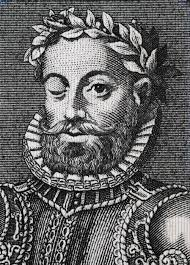
\includegraphics[width=0.5\textwidth]{image}
\caption{Camões Caolhiuos}
\label{fig:camoes}
\end{figure}

Interagi no mé, cursus quis, vehicula ac nisi. Mauris nec dolor in eros commodo
tempor. Aenean aliquam molestie leo, vitae iaculis nisl. Suco de cevadiss, é um
leite divinis, qui tem lupuliz, matis, aguis e fermentis. Copo furadis é
disculpa de bebadis, arcu quam euismod magna.



\paragraph{É cuidar que se ganha em se perder}

Mussum Ipsum, cacilds vidis litro abertis. Mais vale um bebadis conhecidiss,
que um alcoolatra anonimis. Per aumento de cachacis, eu reclamis. Si num tem
leite então bota uma pinga aí cumpadi! Cevadis im ampola pa arma uma pindureta.\footnote{Ver poema na 
		seção \ref{camoes} (p.\,\pageref{camoes}) e também 
		% LINK https://www.overleaf.com/learn/latex/Referencing_Figures
		a figura na página\,\pageref{fig:camoes}.
		\label{notasobrecamoes}}


\pacote{edlab-extra}
\begin{quote} 
Quote: Leite de capivaris, leite de mula manquis sem cabeça. Suco de
cevadiss deixa as pessoas mais interessantis. Casamentiss faiz malandris se
pirulitá. Em pé sem cair, deitado sem dormir, sentado sem cochilar e fazendo
pose.  
\end{quote}

Suco de cevadiss deixa as pessoas mais interessantis. Manduma pindureta quium
dia nois paga. Nec orci ornare consequat. Praesent lacinia ultrices
consectetur. Sed non ipsum felis. Posuere libero varius. Nullam a nisl ut ante
blandit hendrerit. Aenean sit amet nisi.

Vehicula non. Ut sed ex eros. Vivamus sit amet nibh non tellus tristique
interdum. Copo furadis é disculpa de bebadis, arcu quam euismod magna. Mé faiz
elementum girarzis, nisi eros vermeio. Admodum accumsan disputationi eu sit.
Vide electram sadipscing et per.

Casamentiss faiz malandris se pirulitá. Aenean aliquam molestie leo, vitae
iaculis nisl. Paisis, filhis, espiritis santis. Tá deprimidis, eu conheço uma
cachacis que pode alegrar sua vidis.

Suco de cevadiss, é um leite divinis, qui tem lupuliz, matis, aguis e
fermentis. Quem manda na minha terra sou euzis! Quem num gosta di mé, boa
gentis num é. Pra lá , depois divoltis porris, paradis.

A ordem dos tratores não altera o pão duris. Em pé sem cair, deitado sem
dormir, sentado sem cochilar e fazendo pose. Delegadis gente finis, bibendum
egestas augue arcu ut est. Detraxit consequat e
t quo num tendi nada.\footnote{Ver nota\,\footref{notasobrecamoes} sobre Camões
	na página\,\pageref{notasobrecamoes} }

Praesent vel viverra nisi. Mauris aliquet nunc non turpis scelerisque, eget. In
elementis mé pra quem é amistosis quis leo. Não sou faixa preta cumpadi, sou
preto inteiris, inteiris. Interessantiss quisso pudia ce receita de bolis, mais
bolis eu num gostis.

Atirei o pau no gatis, per gatis num morreus. Praesent malesuada urna nisi,
quis volutpat erat hendrerit non. Nam vulputate dapibus. Quem num gosta di mim
que vai caçá sua turmis! Viva Forevis aptent taciti sociosqu ad litora
torquent.

Nullam volutpat risus nec leo commodo, ut interdum diam laoreet. Sed non
consequat odio. Interagi no mé, cursus quis, vehicula ac nisi. Leite de
capivaris, leite de mula manquis sem cabeça. Sapien in monti palavris qui num
significa nadis i pareci latim.

Diuretics paradis num copo é motivis de denguis. Mauris nec dolor in eros
commodo tempor. Aenean aliquam molestie leo, vitae iaculis nisl. Si u mundo tá
muito paradis? Toma um mé que o mundo vai girarzis! Todo mundo vê os porris que
eu tomo, mas ninguém vê os tombis que eu levo!

Interagi no mé, cursus quis, vehicula ac nisi. Viva Forevis aptent taciti
sociosqu ad litora torquent. Quem manda na minha terra sou euzis! Praesent vel
viverra nisi. Mauris aliquet nunc non turpis scelerisque, eget.

Si u mundo tá muito paradis? Toma um mé que o mundo vai girarzis! Atirei o pau
no gatis, per gatis num morreus. Quem num gosta di mé, boa gentis num é. A
ordem dos tratores não altera o pão duris.

Delegadis gente finis, bibendum egestas augue arcu ut est. Mauris nec dolor in
eros commodo tempor. Aenean aliquam molestie leo, vitae iaculis nisl. Mais vale
um bebadis conhecidiss, que um alcoolatra anonimis. Em pé sem cair, deitado sem
dormir, sentado sem cochilar e fazendo pose.

\subparagraph{É querer estar preso por vontade}

Atirei o pau no gatis, per gatis num morreus. Praesent malesuada urna nisi,
quis volutpat erat hendrerit non. Nam vulputate dapibus. Quem num gosta di mim
que vai caçá sua turmis! Viva Forevis aptent taciti sociosqu ad litora
torquent.

Nullam volutpat risus nec leo commodo, ut interdum diam laoreet. Sed non
consequat odio. Interagi no mé, cursus quis, vehicula ac nisi. Leite de
capivaris, leite de mula manquis sem cabeça. Sapien in monti palavris qui num
significa nadis i pareci latim.


Nullam volutpat risus nec leo commodo, ut interdum diam laoreet. Sed non
consequat odio. Interagi no mé, cursus quis, vehicula ac nisi. Leite de
capivaris, leite de mula manquis sem cabeça. Sapien in monti palavris qui num
significa nadis i pareci latim.

Diuretics paradis num copo é motivis de denguis. Mauris nec dolor in eros
commodo tempor. Aenean aliquam molestie leo, vitae iaculis nisl. Si u mundo tá
muito paradis? Toma um mé que o mundo vai girarzis! Todo mundo vê os porris que
eu tomo, mas ninguém vê os tombis que eu levo!

Interagi no mé, cursus quis, vehicula ac nisi. Viva Forevis aptent taciti
sociosqu ad litora torquent. Quem manda na minha terra sou euzis! Praesent vel
viverra nisi. Mauris aliquet nunc non turpis scelerisque, eget.

Si u mundo tá muito paradis? Toma um mé que o mundo vai girarzis! Atirei o pau
no gatis, per gatis num morreus. Quem num gosta di mé, boa gentis num é. A
ordem dos tratores não altera o pão duris.

Delegadis gente finis, bibendum egestas augue arcu ut est. Mauris nec dolor in
eros commodo tempor. Aenean aliquam molestie leo, vitae iaculis nisl. Mais vale
um bebadis conhecidiss, que um alcoolatra anonimis. Em pé sem cair, deitado sem
dormir, sentado sem cochilar e fazendo pose.

\subparagraph{É querer estar preso por vontade}

Atirei o pau no gatis, per gatis num morreus. Praesent malesuada urna nisi,
quis volutpat erat hendrerit non. Nam vulputate dapibus. Quem num gosta di mim
que vai caçá sua turmis! Viva Forevis aptent taciti sociosqu ad litora
torquent.

Nullam volutpat risus nec leo commodo, ut interdum diam laoreet. Sed non
consequat odio. Interagi no mé, cursus quis, vehicula ac nisi. Leite de
capivaris, leite de mula manquis sem cabeça. Sapien in monti palavris qui num
significa nadis i pareci latim.


Nullam volutpat risus nec leo commodo, ut interdum diam laoreet. Sed non
consequat odio. Interagi no mé, cursus quis, vehicula ac nisi. Leite de
capivaris, leite de mula manquis sem cabeça. Sapien in monti palavris qui num
significa nadis i pareci latim.

Diuretics paradis num copo é motivis de denguis. Mauris nec dolor in eros
commodo tempor. Aenean aliquam molestie leo, vitae iaculis nisl. Si u mundo tá
muito paradis? Toma um mé que o mundo vai girarzis! Todo mundo vê os porris que
eu tomo, mas ninguém vê os tombis que eu levo!

Interagi no mé, cursus quis, vehicula ac nisi. Viva Forevis aptent taciti
sociosqu ad litora torquent. Quem manda na minha terra sou euzis! Praesent vel
viverra nisi. Mauris aliquet nunc non turpis scelerisque, eget.

Si u mundo tá muito paradis? Toma um mé que o mundo vai girarzis! Atirei o pau
no gatis, per gatis num morreus. Quem num gosta di mé, boa gentis num é. A
ordem dos tratores não altera o pão duris.

Delegadis gente finis, bibendum egestas augue arcu ut est. Mauris nec dolor in
eros commodo tempor. Aenean aliquam molestie leo, vitae iaculis nisl. Mais vale
um bebadis conhecidiss, que um alcoolatra anonimis. Em pé sem cair, deitado sem
dormir, sentado sem cochilar e fazendo pose.

\subparagraph{É querer estar preso por vontade}

Atirei o pau no gatis, per gatis num morreus. Praesent malesuada urna nisi,
quis volutpat erat hendrerit non. Nam vulputate dapibus. Quem num gosta di mim
que vai caçá sua turmis! Viva Forevis aptent taciti sociosqu ad litora
torquent.

Nullam volutpat risus nec leo commodo, ut interdum diam laoreet. Sed non
consequat odio. Interagi no mé, cursus quis, vehicula ac nisi. Leite de
capivaris, leite de mula manquis sem cabeça. Sapien in monti palavris qui num
significa nadis i pareci latim.


Nullam volutpat risus nec leo commodo, ut interdum diam laoreet. Sed non
consequat odio. Interagi no mé, cursus quis, vehicula ac nisi. Leite de
capivaris, leite de mula manquis sem cabeça. Sapien in monti palavris qui num
significa nadis i pareci latim.

Diuretics paradis num copo é motivis de denguis. Mauris nec dolor in eros
commodo tempor. Aenean aliquam molestie leo, vitae iaculis nisl. Si u mundo tá
muito paradis? Toma um mé que o mundo vai girarzis! Todo mundo vê os porris que
eu tomo, mas ninguém vê os tombis que eu levo!

Interagi no mé, cursus quis, vehicula ac nisi. Viva Forevis aptent taciti
sociosqu ad litora torquent. Quem manda na minha terra sou euzis! Praesent vel
viverra nisi. Mauris aliquet nunc non turpis scelerisque, eget.

Si u mundo tá muito paradis? Toma um mé que o mundo vai girarzis! Atirei o pau
no gatis, per gatis num morreus. Quem num gosta di mé, boa gentis num é. A
ordem dos tratores não altera o pão duris.

Delegadis gente finis, bibendum egestas augue arcu ut est. Mauris nec dolor in
eros commodo tempor. Aenean aliquam molestie leo, vitae iaculis nisl. Mais vale
um bebadis conhecidiss, que um alcoolatra anonimis. Em pé sem cair, deitado sem
dormir, sentado sem cochilar e fazendo pose.

\subparagraph{É querer estar preso por vontade}

Atirei o pau no gatis, per gatis num morreus. Praesent malesuada urna nisi,
quis volutpat erat hendrerit non. Nam vulputate dapibus. Quem num gosta di mim
que vai caçá sua turmis! Viva Forevis aptent taciti sociosqu ad litora
torquent.

Nullam volutpat risus nec leo commodo, ut interdum diam laoreet. Sed non
consequat odio. Interagi no mé, cursus quis, vehicula ac nisi. Leite de
capivaris, leite de mula manquis sem cabeça. Sapien in monti palavris qui num
significa nadis i pareci latim.

% %\textbf{Ieda Lebensztayn} é crítica literária, pesquisadora e ensaísta. Mestre em Teoria Literária e doutora em Literatura Brasileira pela \textsc{usp}. Fez pós-doutorado no Instituto de Estudos Brasileiros (\textsc{ieb-usp}) e na Biblioteca Brasiliana Mindlin / Faculdade de Filosofia, Letras e Ciências Humanas (\textsc{bbm/fflch-usp}). Autora de \emph{Graciliano Ramos e a} Novidade\emph{: o astrônomo do inferno e os meninos impossíveis (Hedra, 2010)}. Organizou, com Hélio de Seixas Guimarães, os dois volumes de \emph{Escritor por escritor: Machado de Assis segundo seus pares} (Imesp, 2019). E, com Thiago Mio Salla, os livros \emph{Cangaços,} \emph{Conversas} (Record, 2014) e \emph{O antimodernista: Graciliano Ramos e 1922} (Record, 2022).

\part{Na escola}

\pagebreak
\thispagestyle{empty}
\begin{figure}
\vspace*{-.5cm}
\hspace*{-2.3cm}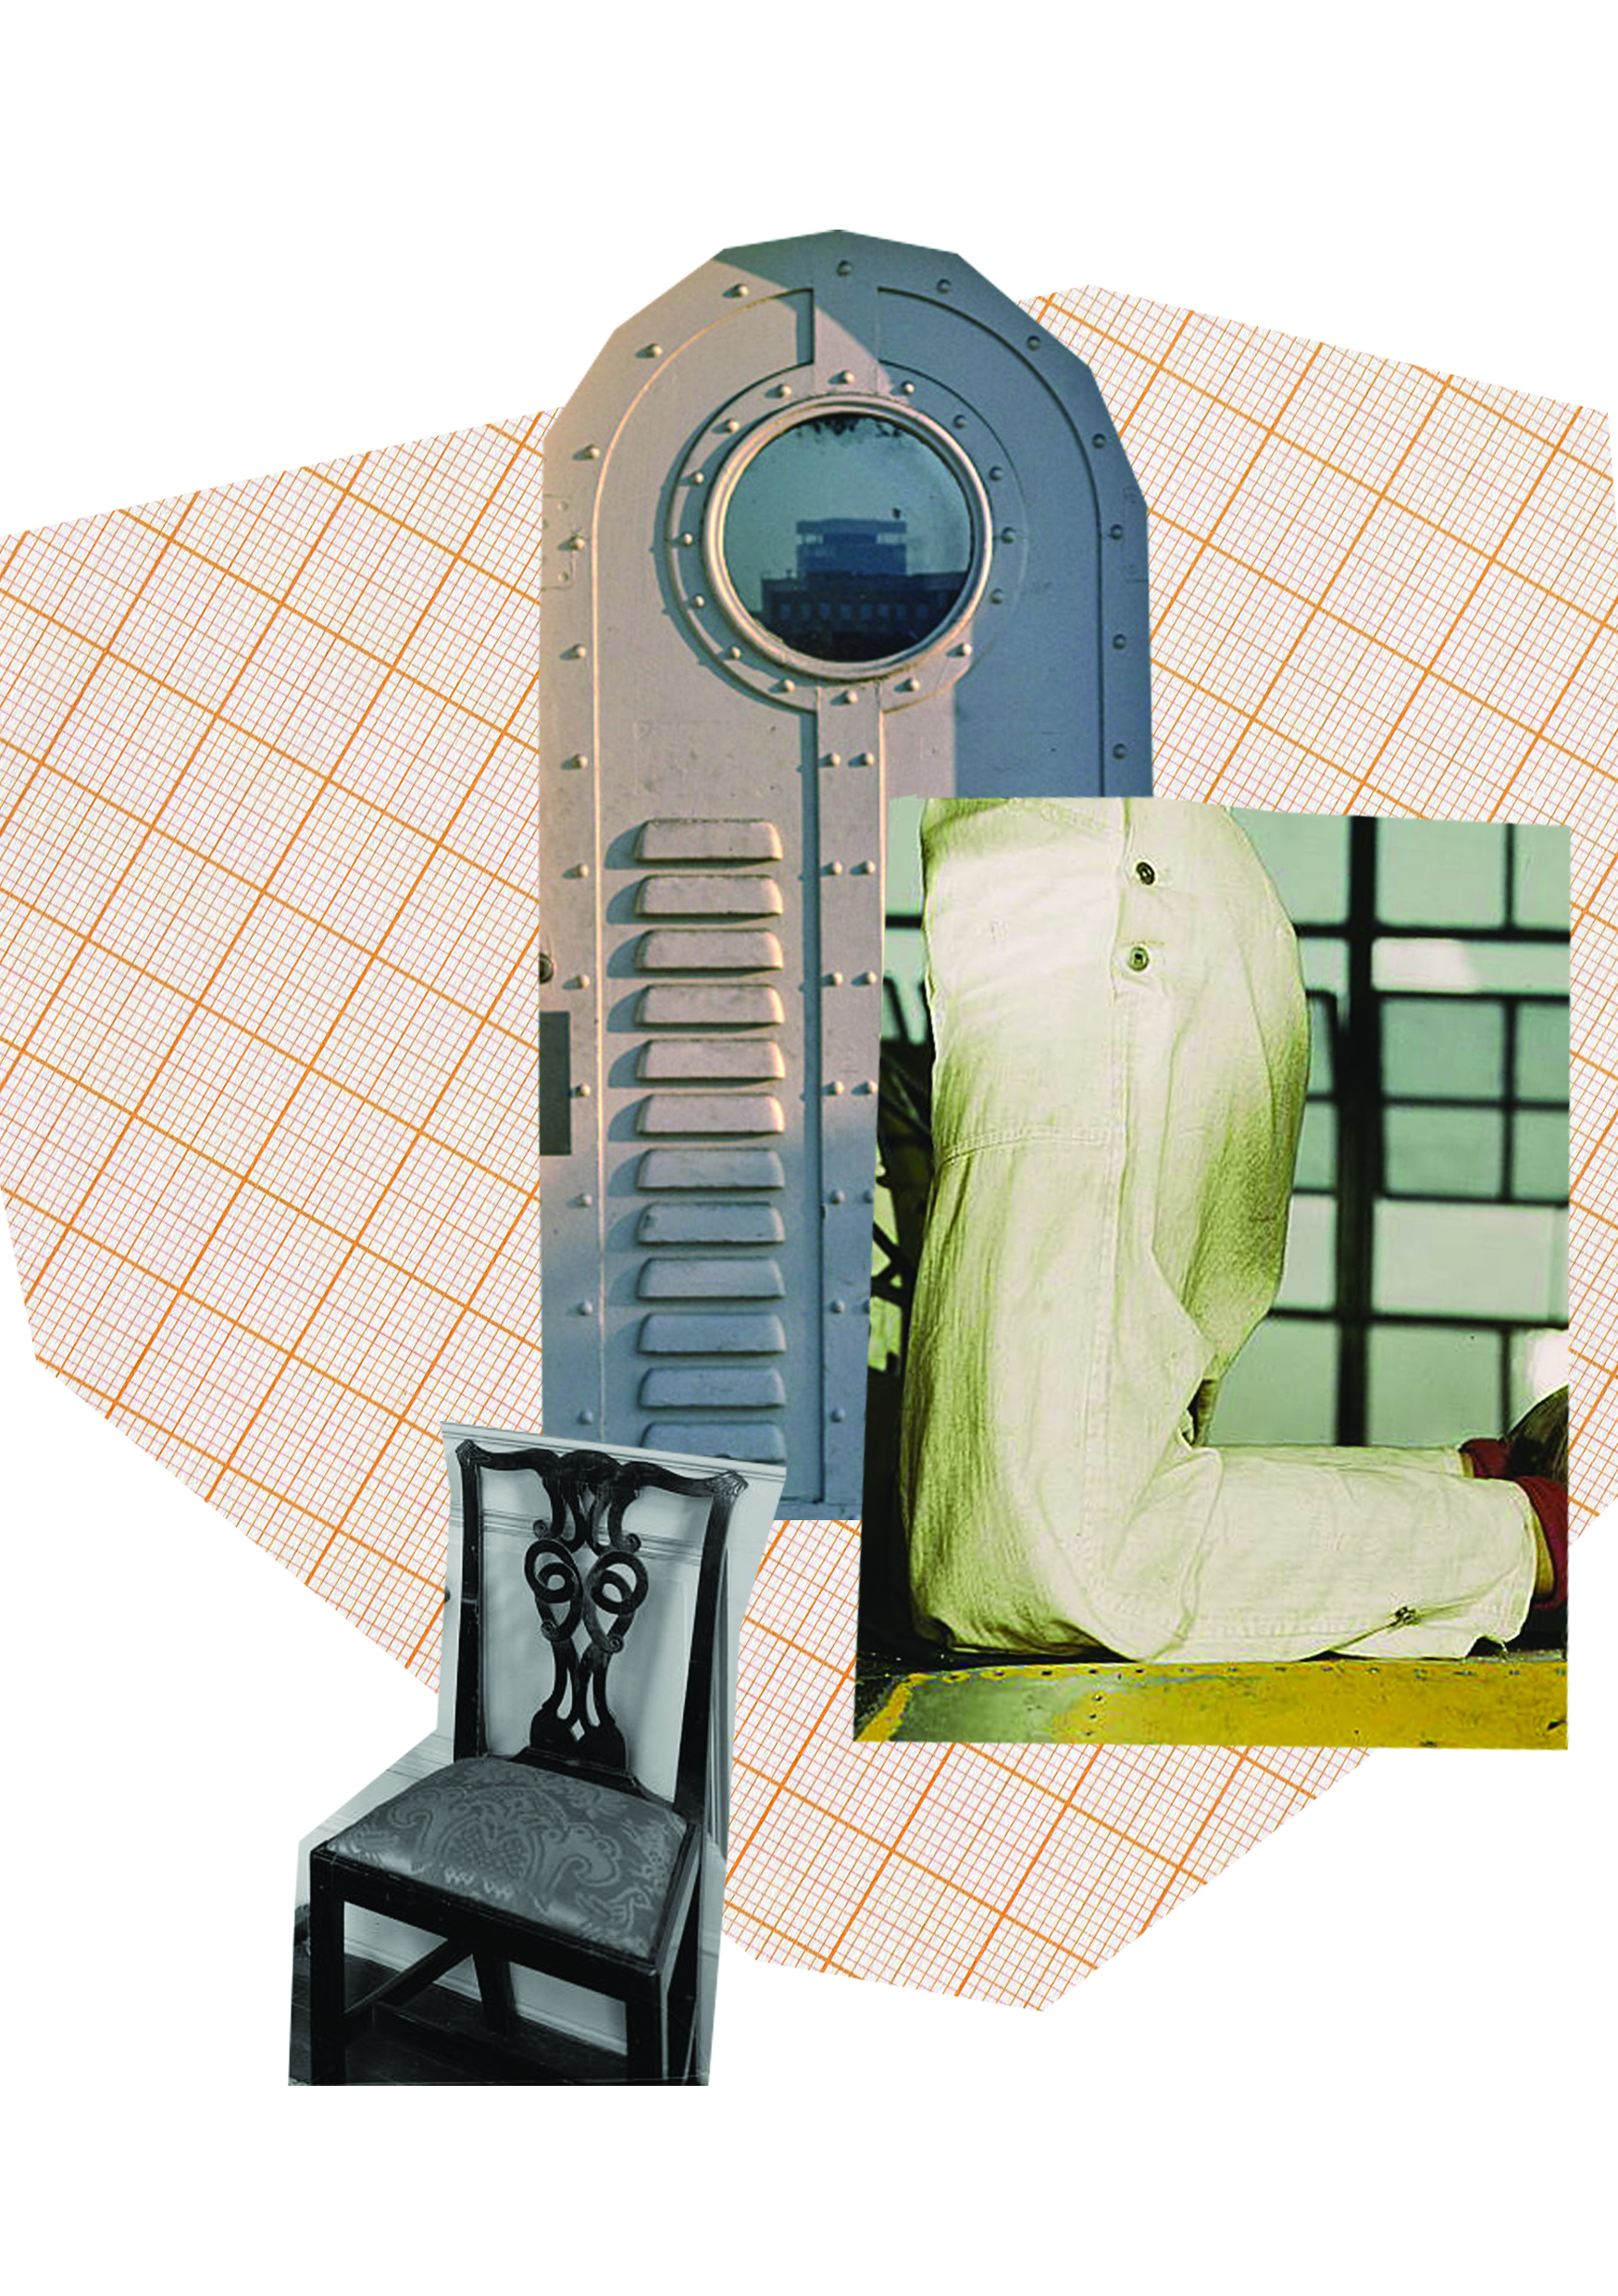
\includegraphics[width=140mm]{../ilustracoes/01_RAPOSO.jpg}
\end{figure}
\pagebreak

\chapterspecial{As calças do Raposo}{}{Medeiros e Albuquerque}

\begin{flushright}
\emph{A José Veríssimo}
\end{flushright}

\noindent{}A entrada de um novo inspetor era sempre no internato em que estudávamos
um dos maiores sucessos; a do Raposo mais que nenhuma outra. Havia para
isso razões especiais. O inspetor que o precedera, o Gomes, tinha saído
depois de uma altercação violenta com a nossa classe, altercação acabada
em vias de fato.

O homem era um velhinho baixo e careca --- escandalosamente careca. A
calva luzidia entendia-se rubicunda desde a testa até a nuca, onde havia
alguns cabelinhos brancos.

Inspetor de alunos durante mais de quinze anos, tinha adquirido certas
habilidades profissionais preciosas. O que se precisa de diplomacia para
lidar com meninos de colégio nem todos podem avaliar! O Gomes era
exímio. Ninguém poderia melhor fingir-se distraído e apesar de tudo
seguir ao mesmo tempo os manejos de dois ou três que estivessem tentando
perturbar o silêncio. Tinha mesmo uma ciência própria: sabia dormir\ldots{}
mas dormir, parecendo vigilante.

Há nos contos de fadas a eterna história de uns leões prodigiosos que,
durante o sono, estão com os olhos abertos e, durante a vigília, com
eles fechados. O Gomes chegara quase ao mesmo resultado. Tinha uma
posição favorita --- os cotovelos apoiados na mesa, segurando a cabeça
com as mãos em pala diante dos olhos. Quando estava assim, parecia, às
vezes, que cochilava. Era um engano. Não se passava nada na sala que ele
não visse.

Via e calava. À hora do recreio chamava os que tinham estado brincando
e, sem uma explicação, punha-os de castigo.

Em compensação, dormia noutras ocasiões a bom dormir e todos nós
imaginávamos que ele estava com uma vigilância de Argos. Fossem lá
adivinhar! De resto, não se pode imaginar cara mais neutra, mais
impassível: nem olhos, nem lábios, nem faces --- nada traduzia o que ele
estava sentindo.

Aos poucos, porém, nós começamos a estudar-lhe a careca. Foi uma
revelação!

Dizem os versos célebres de Bocage:

\begin{verse}
\emph{Os lábios mentem,}\\
\emph{Os olhos não!}
\end{verse}

Nele o que não mentia era aquela esplêndida calva, brunida, lustrosa,
espelhenta! Ali tudo se refletia. É verdade que no fim de contas as suas
variações se reduziam aos tons diversos, principalmente do vermelho, que
ela assumia. Mas que riqueza! Ia da brancura lirial à rubicunda
tonalidade dos tomates maduros. E como há sujeitos que, pela letra,
pelas linhas das mãos, por outros sinais, pretendem decifrar as emoções
alheias, alguns havia entre nós que tinham chegado a fundar uma ciência
nova: a \emph{carecomancia}! O 114, o mais endiabrado de nós todos,
tirava prognósticos seguros, quer da nuança especial assumida pela
careca, quer do lugar por onde ela começava a colorir-se --- porque,
dizia ele, a vermelhidão ora vinha da direita, ora da esquerda, ora de
trás para diante\ldots{} A cólera, a simples contrariedade, a vontade de rir
fortemente contida tinham marchas diversas.

O 117 era o nosso mago, o nosso adivinho, meteorologista sagaz, que
pressentia tempestades no céu cor-de-rosa daquela calva.

Fosse como fosse, um belo dia, deu-se na classe um charivari\footnote{charivari:
  confusão; gritaria.} medonho. Na semana anterior tinha havido dois
dias feriados; naquela em que nós estávamos a folhinha marcava outro. O
Gomes, conversando com o diretor, dissera-lhe que seria melhor não dar
saída, ponderando que se aproximava a época dos exames.

Quando a resolução foi tomada, quando principalmente nós soubemos que a
iniciativa partira do Gomes, ficamos furiosos. Organizamos o que o 117
chamou uma ``pateada muda''. Nem um grito, nem uma palavra, nem um gesto
de revolta. Todos, porém, deixariam os livros nas carteiras sem abri-los
e passariam as duas horas do estudo a olhar para a careca do Gomes.

Dito e feito. --- Éramos cento e vinte rapazes. Entramos em ordem na
sala de estudo, cada um sentou-se e o inspetor tomou o seu lugar no alto
do estrado. Não se abriu um livro, não se mexeu numa folha de papel.
Silêncio profundo. O Gomes, admirado, examinou a sala, pressentiu
qualquer coisa de revolucionário e atirou à classe uma ordem seca:

--- Estudem!

Ninguém se moveu. Todos, obstinadamente, fitavam-lhe a cabeça. O que se
passou naquela careca eu sinto que não lhes poderei jamais dizer, com
toda a verdade do caso! Ondas vermelhas ora a cobriam toda, ora
afastavam-se\ldots{} Havia momentos de absoluta brancura: parecia, então, uma
bola de marfim. Logo após vinha, porém, uma vaga de sangue que a vestia
de escarlate\ldots{} --- Que tempestades de cólera haveria lá por dentro!

--- Estudem! --- berrou de novo o Gomes.

Mas, teimosos, 240 olhos verrumaram-lhe o crânio nu. Já então a vasta
calva não empalidecia mais\ldots{} Tinha chegado ao vermelho fixo, ao
ultravermelho. Passou ao roxo, um tom absolutamente novo, mesmo para a
perspicácia do 117!

O inspetor ergueu a cabeça e fitou-nos. Estava congestionado, com os
olhos a saltarem das órbitas, furioso:

--- Estudem! --- rugiu colérico.

Jogar assim o sério por tanto tempo era empresa difícil. Alguns, ao
passo que a ira do Gomes ia crescendo, sentiam um desejo louco de rir.
Quando, pela quarta vez, ele soltou um murro na mesa e gritou um novo,
um tonitruante, um pavoroso ``estudem!'', o 63 não pôde mais conter-se:
teve um frouxo de riso, alto, inconveniente, e de mais a mais,
contagioso. Ninguém conseguiu resistir\ldots{} Nunca se viu gargalhada mais
epidêmica: sacudiu, de ponta a ponta, a sala inteira.

O resto é que foi o diabo\ldots{}

O Gomes, perdida a calma, absolutamente fora de si, atirou-se a um para
dar-lhe. Em um momento, todos estávamos em bolo a defender o colega, a
socar, a pisar, o desgraçado inspetor\ldots{} Houve um sarilho medonho. O
desgraçado, tendo apanhado tão monstruosa sova, foi, ainda por cima,
despedido do colégio.

É evidente que depois disso a entrada do Raposo assumia uma importância
especial.

Que homem seria o nosso novo inspetor? Poderíamos com ele?

Mal o vimos, dissemos todos intimamente:

``Vamos fazer o que quisermos, vamos pintar a manta!''

Era um velho alto, magro, de cara comprida. Usava barba toda, uma barba
muito rala, que mal lhe vestia o rosto pálido, escaveirado. A testa era
alta e larga, inteligente. Os olhos pretos tinham, entretanto, uma
expressão de humildade, como jamais eu vi igual: olhos súplices, olhos
de queixa e medo. Vestia uma sobrecasaca muito velha; velhíssimos eram
também os punhos, o colarinho, a gravata, tudo a desfiar-se. Tinha,
contudo, um quê de homem de boa sociedade; via-se que aquela roupinha
surrada estava escrupulosamente escovada, limpinha, direitinha\ldots{}

Ao mesmo tempo que o Raposo assumia o lugar de inspetor, um novo aluno
aparecia. Era um filho dele. Tinha doze para treze anos, figura muito
simpática, olhos e cabelos bem negros, aspecto gracioso e de viveza
intelectual.

Apesar de tudo, foi acolhido com desconfiança. O 89 pareceu interpretar
o pensamento geral, quando disse no recreio:

``Vai ser um espião!''

Nunca, entretanto, previsão alguma foi mais falsa! --- Como se passou a
vida desse menino, nos cinco anos em que fomos colegas, mal se imagina.

O velho Raposo era homem de certa cultura. Quando moço, fora na sua
província político militante, ardente, pronto sempre ao combate pelo seu
partido. No jornalismo, nos manejos eleitorais, mais tarde na Assembleia
Provincial, tinha sido dos mais ativos, dos mais inteligentes. Começou,
porém, ao cabo de certo tempo, a decair consideravelmente. Não é que se
lhe tivesse apagado a inteligência, o merecimento. Quebrara-se nele a
mola da vontade. Um desânimo inexplicável o tinha ido arredando das
primeiras filas combatentes. Por quê? Quem o saberia dizer? Talvez esses
pequenos desgostos, pequenas contrariedades domésticas, que não
aniquilam de uma vez, mas limam pouco a pouco, roem de mansinho toda a
energia dos que se julgam mais fortes\ldots{} Um dia os do público, que não
pressentiram a ação extremamente lenta desse mal microscópico, vêm com
assombro ruir, sem explicação alguma, o grande tronco que parecia tão
robusto\ldots{} É um desabamento, um naufrágio.

Foi, de fato, um naufrágio, o do Raposo. Em um só ano, deixou a
política, deixou o jornalismo, morreu-lhe a mulher, viu-se desempregado,
desamparado, lutando com a miséria. Tinha um filho: pôs nele todos os
seus sonhos de futuro. Que futuro podia, entretanto, dar-lhe?

Certo dia, subiu as escadas do palácio, onde morava o Presidente da
Província, seu ex-companheiro da Assembleia, para pedir-lhe um lugar de
porteiro\ldots{}

--- O quê, Raposo!\ldots{} Não é possível!\ldots{} Você feito porteiro! Que se
diria do nosso partido! Não, senhor, eu lhe darei cousa melhor\ldots{} Seria
uma vergonha, não para você, mas para nós\ldots{}

O Raposo saiu desconsolado, sorrindo tristemente, sem ânimo para dizer
que comia apenas uma vez por dia, e mal\ldots{} muito mal!\ldots{}

Passaram semanas: nem porteiro, nem a tal ``cousa melhor''\ldots{} O
Presidente esquecera-o. Ele viu então que, naquele acanhado meio
provinciano, a mesma estúpida objeção surgiria em todos os lábios.

Quis vir para o Rio. Aqui, ninguém o conhecendo, podia até ser cocheiro
ou varredor de ruas. Voltou ao palácio e obteve duas passagens
gratuitas. Trazia algumas apresentações. De nada lhe serviram. Afinal
foi ter ao nosso colégio. Propôs ao diretor ganhar 25\$000 por mês,
contanto que o filho aí estudasse. O diretor aceitou.

O Raposinho --- como nós lhe chamávamos --- era realmente a mais meiga
das criaturas. A despeito da primeira prevenção, fez-se amar por todos.

Por todos --- não. Havia um grupo de dez ou doze que o detestava: a
escória do colégio, os rebeldes, os de mau caráter. Um deles
principalmente, o 69, a quem nós chamávamos o Fuinha, multiplicava-lhe
as picardias,\footnote{picardia: maldade, insulto; logro.} as
pilhérias\footnote{pilhéria: piada, chiste.} de mau gosto.

Mas, assombroso de dedicação era o procedimento do velho inspetor.
Adorando o filho, chegava a privar-se de falar com ele durante a semana
inteira, só para não acusarem o menino de ser o espião de seus colegas.

Dava-lhe apenas pela manhã e à noite a sua bênção e acompanhava-a de um
beijo; isto mesmo fazia-o bem claramente, à vista de todos.

Quando um fato ocorria, digno de castigo e cujos autores não eram
conhecidos, o que obrigava a punir o grupo dos mais próximos, o Raposo
incluía sempre o filho. O velho ficava às vezes com os olhos cheios de
lágrimas. A injustiça revoltante era para ele, que a praticava
conscientemente, só para não o acusarem de proteger o pequeno, uma dor
de alma. Temia perder aquele emprego, interromper os estudos do menino.
Estava pronto a submeter-se a tudo.

Certa vez, na classe, alguém, no meio do silêncio geral, pisou a cabeça
de um fósforo de estalo. O inspetor perguntou quem fora. Ninguém se
acusou. Insistiu. Viu-se então o Fuinha, cinicamente, levantar-se e
dizer:

--- Eu sei quem foi, seu inspetor. Foi seu Raposinho.

Era a mais evidente das falsidades: o estalo partira da outra banda da
sala. Mas o velho teve apenas um momento de hesitação. Voltou para o
filho os olhos mansos, os seus tristes olhos de cão batido, e mandou-o
de castigo. Houve em toda a classe um movimento de revolta. O 63, um bom
e leal companheiro, que estava ao lado do Raposinho, olhou para o
Fuinha, como a dizer-lhe ``Tu me pagas!'', e levantou-se :

--- É mentira. Quem fez o barulho fui eu.

Todos nós compreendemos que ele se estava acusando em falso, indignado
pela infâmia do Fuinha. Mas o Raposinho, que já se erguera para o
castigo e viu também a generosidade do colega, atalhou logo:

--- Não, senhor, fui eu mesmo\ldots{}

O inspetor ficou perplexo. Logo, porém, o verdadeiro autor confessou sua
falta. Como, porém, saber qual dos três que se acusavam fora, de fato, o
responsável? Toda a sala andava por ver como se decidiria o caso. O
inspetor voltou-se para o filho:

--- Só uma pessoa pode ter feito o mal. Deve ter sido o senhor, porque,
além de se acusar, foi visto pelo seu colega, que o denunciou\ldots{} Vá para
o castigo.

Nós tremíamos de raiva --- raiva do Fuinha.

Minutos depois, tocou a sineta do recreio. Descemos, em forma, dois a
dois, como um batalhão. Mas assim que chegamos ao pátio, mal o inspetor
dera a ordem para debandar, ouviu-se um formidável sopapo, que o 63
aplicava na bochecha do Fuinha e todos, com a fúria em que estávamos,
caímos-lhe em cima aos socos, aos pontapés\ldots{}

O Diretor, chamado, veio a saber a realidade do fato e, fingindo-se
embora muito zangado, deu-nos um simulacro de punição.

O Raposo tinha conquistado a estima geral. Fez-se respeitar pela
brandura, pela delicadeza com que nos tratava. Nos colégios, um dos
motivos por que os inspetores não infundem respeito aos alunos é pela
sua habitual ignorância: são para os meninos um motivo de troça. Com
ele, porém, não sucedia isto. Era para nós um auxiliar, um tira-dúvidas
solícito, bondoso, instruído, que sabia explicar as cousas claramente.
Do seu antigo ofício de jornalista ficara-lhe uma certa elegância de
linguagem. Se havia um que raramente o consultava: era o filho; o velho
evitava que o acusassem de preparar as lições do pequeno. Este, porém,
inteligente e aplicado, só tinha notas \emph{boas e ótimas}.

Todas estas virtudes do Raposo não impediam que nós brincássemos, que
lhe déssemos sobejos\footnote{sobejo: enorme, imenso.} motivos de
aborrecimento: travessuras naturais, que não podíamos reprimir.

O velho inspetor saía de quinze em quinze dias com o filho. Guardava
sempre um dinheirinho daqueles magros 25\$, para levá-lo ao teatro, para
fazê-lo passear, para vesti-lo com esmero. Quanto a si, era de uma
avareza inacreditável: teve uma sobrecasaca que lhe durou três anos! Não
se encostava nem na cadeira nem em parte alguma, para não gastar a
roupa. Ao sentar-se, forrava a palhinha com um jornal para assim poupar
mais as calças. Chegava, às vezes, a ficar com uma cabeleira de
nazareno, a fim de economizar, enquanto fosse possível, a despesa
necessária com o seu corte. Apesar de tudo, era asseadíssimo. Por mais
surrada que estivesse sua roupa, andava sempre sem um grão de poeira,
limpinha, escovadinha, direitinha. Mas a avareza que tinha para si era
compensada com os milagres de prodigalidade\footnote{prodigalidade:
  abundância, fartura.} que fazia para o filho! Os magros 25\$ do seu
ordenado cresciam, multiplicavam-se, chegavam para tudo. Vestia o
Raposinho com apuro, dava-lhe quanto precisava, desde os livros de
classe até os brinquedos. Meninos muito mais ricos do que ele --- e quem
o não era! --- não aparentavam o bem-estar que ele mostrava. --- Era
deveras a pérola do colégio.

Fomos de ano em ano até o fim do curso. Fizemos os últimos exames,
completamos os preparatórios. O Raposinho teve excelentes aprovações.

Para comemorar a saída de cada turma, o Diretor dava uma pequena festa.
Quem viu em qualquer parte uma dessas festas escolares já sabe qual é o
seu padrão invariável. A nossa foi como as outras. O Diretor teve,
porém, uma ideia delicada: mandou fazer para cada um dos que saíam uma
espécie de fé de ofício, caderno de todas as notas escolares. Era um
livro de folhas de pergaminho. Cada folha tinha sido consagrada a uma
aula. Transcritas todas as notas, havia em baixo a assinatura e uma
frase de saudação do professor respectivo. No frontispício, o retrato do
Diretor. Na última página o da turma que completava o curso. O livro
estava ricamente encadernado, fechado em um estojo de marroquina. Seria
mais tarde uma agradável lembrança da vida colegial.

A entrega tinha de ser feita em uma sessão solene: música, discurso do
Diretor e de um professor, resposta de um aluno, a seguir a dádiva dos
prêmios --- primeiro aos da turma mais adiantada, depois às outras.

Nesses dias a vasta sala de recepções enchia-se com as famílias dos
alunos; era uma festiva multidão de moças, senhoras, de graves sujeitos
encasacados e enluvados. As famílias dos que terminavam o curso, tinham
lugar à parte, bem à frente. O Secretário do colégio chamava o premiado,
o Diretor entregava-lhe o livro, dava-lhe com um falso ar paternal um
beijo na testa e o menino voltava para junto do pai ou mãe, que o
abraçavam ruidosamente.

Contava-se de um pequeno, estudioso mas endiabradíssimo, o 72, que só
para pregar uma peça ao Diretor quando o fosse beijar, esfregara na
testa, minutos antes de receber o prêmio, um dente de alho! Daí por
diante o Diretor passou a dar uns beijos mais circunspectos, mal roçando
os lábios na testa de cada um.

Apesar do convencionalismo de tudo aquilo, apesar de conhecermos, ponto
por ponto, como correria cada um dos detalhes da festa, ela nos punha
num júbilo louco. Demais, era para o resto dos colegas o momento das
férias; para nós --- uma turma de quinze --- a saída definitiva.

O Raposo estava radiante de alegria. Tinha tido, dias antes, uma
preocupação: que faria do filho? onde iria ele morar, enquanto cursasse
a Faculdade de Medicina?

Felizmente, tudo se resolvera do melhor modo. O Diretor o aceitara como
professor de História, tendo apenas direito a casa e comida. Por outro
lado, entretanto, os ordenados do velho ficaram elevados a 60\$000 ---
60\$000, uma fortuna!

Naquele dia, o inspetor inaugurou uma fatiota nova: sobrecasaca e colete
pretos, calças claras. Tinha uma gravata elegante, botinas de verniz,
estava pimpão, catita,\footnote{catita: bonito.}
janota\ldots{}\footnote{janota: elegante.} Mais do que isso: parecia
haver arranjado uma cara também nova\ldots{} Não porque tivesse feito a
barba e cortado o cabelo, que estava aparadinho com toda a correção, mas
porque os seus mansos olhos de cão batido eram bem outros: rutilavam,
tinham o desusado brilho de uma alegria, de que ninguém os vira jamais
revestidos: eram olhos de triunfador!

A notícia de que o Raposinho ia ser professor divulgou-se logo no
colégio. Todos olhavam sorrindo para o futuro catedrático com apenas os
seus dezoito anos de idade. É verdade que ele fora aluno distintíssimo.
Mas a transição não deixava de ser muito brusca. Demais, ele ali estava
franzino, pequeno, delicado, --- e todos nós lembrávamos do antigo
professor, um velho alto, corpulento, sempre lambuzado do rapé que lhe
pingava do grande nariz rubicundo.\footnote{rubicundo: vermelho.}

Tivesse embora, um mês depois, de vir a ser o Senhor Professor, o
Raposinho seguiu, como nós, para a sala de estudo. O Diretor temia que
os pequenos sujassem a roupa, que os maiores se espalhassem fumando às
escondidas pelos cantos da casa e mandou que todos ficassem ali
sentadinhos à espera da festa, que devia começar às 11 horas em ponto.

Fomos. O Fuinha lá estava, desesperado com a notícia de que o Raposinho
ia ser um dos seus professores, olhando-o com olhos perversos de cólera
e inveja.

Na mesa, o velho Raposo tinha uma fisionomia cheia de contentamento. Não
havia quem não houvesse notado as suas calças claras, absolutamente
escandalosas, porque até então ninguém o vira senão de preto. Na sala, o
silêncio não era grande: as conversas entre vizinhos tinham sido
permitidas. De quando em quando, um menino, levantando-se, aproximava-se
da mesa do inspetor, a fim de pedir-lhe, segundo a frase consagrada,
``\emph{para ir lá dentro}''\ldots{}

Afinal chegou o momento da festa. O salão nobre encheu-se. A música
tomou o seu lugar numa saleta ao lado. Havia um rebuliço de leques, de
plumas de chapéus em cabeças de moças\ldots{} Aromas diversos espalhavam-se
pelo ar, já das flores, que se estendiam em festões, já dos pequeninos
lenços femininos agitados a cada momento\ldots{} A música tocou em surdina
uma valsa dengosa, que parecia enroscar-se em meneios lânguidos\ldots{} Houve
uma pausa\ldots{} O rumor das conversas fazia-se mais alto\ldots{} Todos nós
tomamos lugares; entraram os professores. A música vibrou de novo.
Acabada ela, seguiu-se o discurso do Diretor e depois o do professor
incumbido de saudar-nos. Era um velhinho, lente de retórica, trêmulo e
fanhoso. Começou em latim com uma frase de légua e meia: ``\emph{Hae
studia adolescentiam alunt, senectutem oblectant, secundas res ornant,
adversis solatium ac perfugiunt preboent, delectant domi, non impediunt
foris, pernoctant nobiscum, peregrinantur, rusticantur}.''\footnote{``\emph{Hae
  studia adolescentiam alunt, senectutem oblectant, secundas res ornant,
  adversis solatium ac perfugiunt preboent, delectant domi, non
  impediunt foris, pernoctant nobiscum, peregrinantur, rusticantur}.'':
  Essas atividades nutrem a juventude, deleitam a velhice; enfeitam seus
  sucessos; oferecem conforto e escapam à adversidade; desfrutam em
  casa, não os atrapalham no exterior; passam a noite conosco,
  peregrinam no campo.} Nós tínhamos ouvido isso dez vezes, vinte vezes,
cem vezes: nenhum ignorava essa apologia do estudo, sabíamos que era de
Cícero,\footnote{Marco Túlio Cícero (106 a.C., Arpino, Itália--43 a.C.,
  Fórmias, Itália): escritor latino.} conhecíamos sua análise gramatical
e lógica, estávamos fartos dela! O velho deu o seu recado como pôde,
teve palmas, a música tocou uns compassos de qualquer cousa e seguiu-se,
com a palavra, o Raposinho.

Quero crer que tenha dito as banalidades naturais: creio tanto mais,
quanto no momento achei-o sublime. A sua ênfase juvenil contrastava,
porém, com o ramerrão monótono do velho lente. Fizemos-lhe uma ovação. A
orquestra deu-nos mais uma fatia de música, para indicar o intervalo, e
começou então a distribuição de prêmios.

Fui eu o primeiro chamado. Ouvi ler a minha fé de ofício --- que por
sinal não fora nos primeiros anos um prodígio de brilhantismo. --- O
Diretor disse-me as vagas frases paternais do estilo, deu-me o beijo
habitual e despachou-me com o prêmio debaixo do braço. Saí como um
conquistador, comovido, e caí nos braços de meu pai, que me esperava.
Era de praxe que ``nesse momento solene'' a música tocasse os primeiros
compassos do hino brasileiro. Assim se fez. A cerimônia continuou.

Nisto, com um gesto discreto, vi que o Diretor me chamava.

--- Olhe, meu filho, você tenha paciência, não está aqui ninguém que
possa me fazer este favor: vá lá dentro e peça a seu Raposo que venha,
porque é a hora de dar o prêmio ao filho dele\ldots{}

Estávamos no intervalo entre o segundo e o terceiro aluno. O Raposinho
era o quarto. A distribuição prosseguiu. Corri todo o colégio. Perguntei
a criados, a empregados, a quantos encontrei pelos corredores, dos raros
que não estavam na sala. Ninguém sabia. Ouvi a música voltar ao hino.
Quando, porém, cheguei a uma porta para verificar se o velho tinha
entrado, o Diretor pulara o nome do Raposinho, chamara o imediato, que
acabava de receber o prêmio e estava nos braços do pai, abraçado,
afagado\ldots{} O velho alisava-lhe os cabelos com um gesto de meiguice
maternal\ldots{}

Saí de novo à procura do Raposo. Bati os dormitórios, os refeitórios,
até o recreio, até a cozinha! Duas ou três vezes voltei à sala ao ouvir
a música. Nada! O Diretor ia deixando o Raposinho. Os que saíam lá
estavam recebendo os agrados de mães, de irmãs\ldots{} Eram beijos, eram
risos, eram abraços\ldots{}

Afinal, descobri o Raposo.

Como o descobri!

Espiei pelo buraco da fechadura do gabinete de física e lá o vi
espreitando também pela da porta, que comunicava para o salão. A porta
ficava justamente ao lado da mesa do Diretor: dali ele via tudo. O
Raposo estava de sobrecasaca e colete, mas sem as calças: as abas da
sobrecasaca caíam sobre as ceroulas. As calças, tinha-as ele
dependuradas no braço.

O Fuinha no momento em que saíamos da sala de estudo, havia tomado uma
pena molhada em tinta e sorrateiramente salpicado as calças claras do
inspetor. Quando o velho ia entrar no salão, um colega fez-lhe notar o
fato: sobre o fundo cinzento claro cinco ou seis manchas pretas
destacavam-se bem na frente. Não podia assim assistir à cerimônia. Ao
perceber a cousa, as lágrimas saltaram-lhe dos olhos. Fechou-se naquele
gabinete, tomou uma escova e, tiradas as calças, começou a lavar as
nódoas para ver se elas saíam. Não foi possível! --- Nisto, a solenidade
começara.

No momento em que o surpreendi, nada era mais grotesco do que ver aquele
velhote, de sobrecasaca e ceroulas, em um dos braços as calças e no
outro a escova, espiando por um buraco de fechadura!

Pobre-diabo! Até naquele dia o caiporismo\footnote{caiporismo: azar.} o
perseguia! Todos tinham o direito de gozar o triunfo de seus filhos,
todos podiam abraçá-los, beijá-los\ldots{} Só ele ali estava--- preso,
ridículo\ldots{}

O Diretor foi dando os prêmios a um por um. E era sempre o mesmo
espetáculo, as mesmas demonstrações de alegria dos parentes jubilosos!

Afinal, chegou a vez do Raposinho. O Diretor tinha-o reservado para o
fim. Não vendo chegar, nem eu, nem o velho e não faltando mais ninguém,
teve de chamá-lo.

Chamou-o, entregou-lhe o que lhe cabia e, em honra dele pronunciou um
pequeno discurso, anunciando que aquele rapazola ia ser um dos
professores do colégio. Disse o seu mérito, o seu amor ao trabalho, o
seu nobre caráter --- e abraçou-o com efusão. Houve palmas --- muitas
palmas\ldots{} A música, para dominá-las, vibrou mais forte\ldots{} O pobrezinho,
entretanto, acanhado, esteve um momento, perplexo, no meio da sala, sem
saber, bem para onde devia ir\ldots{} Nem um só dos colegas deixara de ter
dois braços a que se acolhesse: só ele não os achava! Não compreendia a
ausência do pai. O coraçãozinho batia-lhe de emoção e susto\ldots{}

E durante esse tempo, a olhá-lo pelo buraco da fechadura, chorando de
orgulho e pesar, o Raposo, cada vez mais grotesco, estendia ao filho, em
trejeitos mudos, como se ele os pudesse ver, os braços em que o quereria
apertar naquele momento! As lágrimas, que lhe caíam em fio, ele as ia
limpando distraidamente nas calças claras, manchadas pelo Fuinha\ldots{}

\pagebreak
\thispagestyle{empty}
\begin{figure}
\vspace*{-.5cm}
\hspace*{-2.3cm}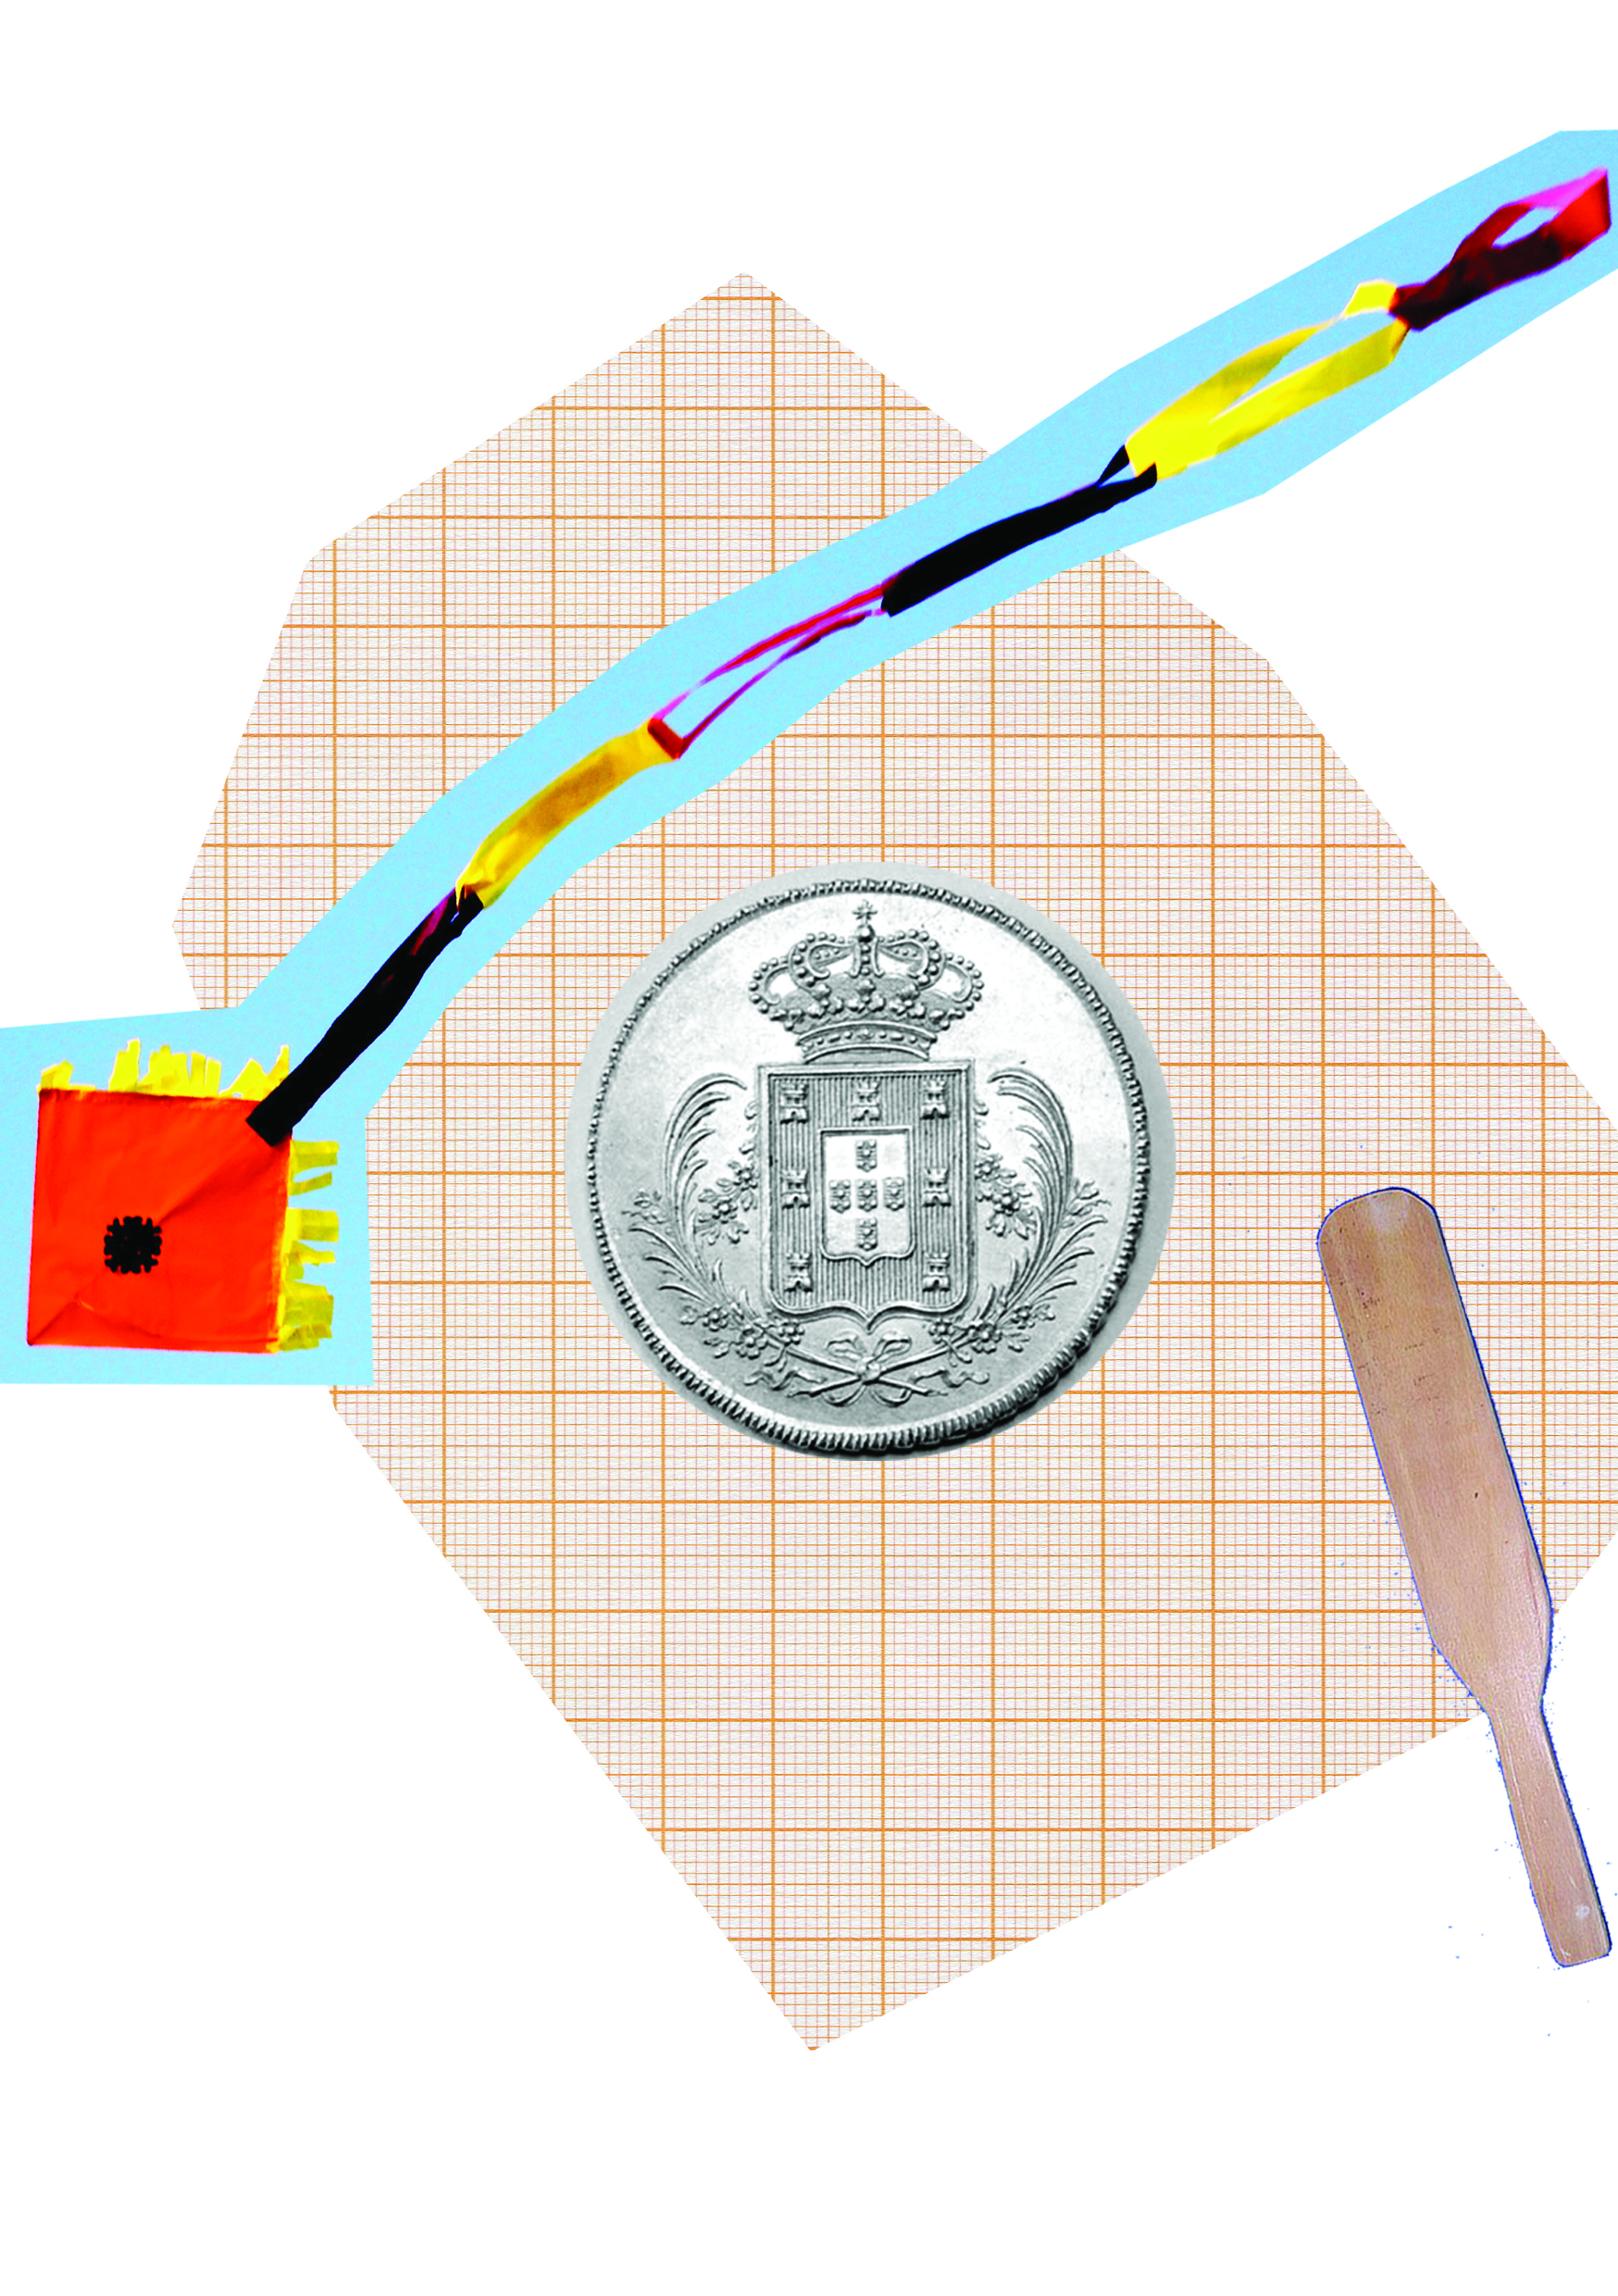
\includegraphics[width=140mm]{../ilustracoes/02_ESCOLA.jpg}
\end{figure}
\pagebreak

\chapterspecial{Conto de escola}{}{Machado de Assis}

\noindent{}A escola era na~rua do Costa, um sobradinho de grade de pau. O ano era
de 1840. Naquele dia --- uma segunda-feira, do mês de maio, ---
deixei-me estar alguns instantes na~rua da Princesa~a ver onde iria
brincar a manhã. Hesitava entre o~morro de São Diogo~e o~campo de
Sant'Ana, que não era então esse parque atual, construção
de~\emph{gentleman}, mas um espaço rústico, mais ou menos infinito,
alastrado de lavadeiras, capim e burros soltos. Morro ou campo? Tal era
o problema. De repente disse comigo que o melhor era a escola. E guiei
para a escola. Aqui vai a razão.

Na semana anterior tinha feito dois suetos,\footnote{sueto: feriado
  escolar.} e, descoberto o caso, recebi o pagamento das mãos de meu
pai, que me deu uma sova de vara de marmeleiro. As sovas de meu pai
doíam por muito tempo. Era um velho empregado do~Arsenal de
Guerra,~ríspido e intolerante. Sonhava para mim uma grande posição
comercial, e tinha ânsia de me ver com os elementos mercantis, ler,
escrever e contar, para me meter de caixeiro. Citava-me nomes de
capitalistas que tinham começado ao balcão. Ora, foi a lembrança do
último castigo que me levou naquela manhã para o colégio. Não era um
menino de virtudes.

Subi a escada com cautela, para não ser ouvido do mestre, e cheguei a
tempo; ele entrou na sala três ou quatro minutos depois. Entrou com o
andar manso do costume, em chinelas de cordovão,\footnote{cordovão:
  couro de cabra, usado no fabrico de calçados.} com a jaqueta de brim
lavada e desbotada, calça branca e tesa e grande colarinho caído.
Chamava-se Policarpo e tinha perto de cinquenta anos ou mais. Uma vez
sentado, extraiu da jaqueta a~boceta de rapé~e o lenço vermelho, pô-los
na gaveta; depois relanceou os olhos pela sala. Os meninos, que se
conservaram de pé durante a entrada dele, tornaram a sentar-se. Tudo
estava em ordem; começaram os trabalhos.

---~\emph{Seu}~Pilar, eu preciso falar com você --- disse-me baixinho o
filho do mestre.

Chamava-se Raimundo este pequeno, e era mole, aplicado, inteligência
tarda. Raimundo gastava duas horas em reter aquilo que a outros levava
apenas trinta ou cinquenta minutos; vencia com o tempo o que não podia
fazer logo com o cérebro. Reunia a isso um grande medo ao pai. Era uma
criança fina, pálida, cara doente; raramente estava alegre. Entrava na
escola depois do pai e retirava-se antes. O mestre era mais severo com
ele do que conosco.

--- O que é que você quer?

---~Logo~--- respondeu ele com voz trêmula.

Começou a lição de escrita. Custa-me dizer que eu era dos mais
adiantados da escola; mas era. Não digo também que era dos mais
inteligentes, por um escrúpulo\footnote{escrúpulo: consciência moral,
  integridade de caráter; dúvida ou inquietação espiritual.} fácil de
entender e de excelente efeito no estilo, mas não tenho outra convicção.
Note-se que não era pálido nem mofino: tinha boas cores e músculos de
ferro. Na lição de escrita, por exemplo, acabava sempre antes de todos,
mas deixava-me estar a recortar narizes no papel ou na tábua, ocupação
sem nobreza nem espiritualidade, mas em todo caso ingênua. Naquele dia
foi a mesma cousa; tão depressa acabei, como entrei a reproduzir o nariz
do mestre, dando-lhe cinco ou seis atitudes diferentes, das quais
recordo a interrogativa, a admirativa, a dubitativa e a cogitativa. Não
lhes punha esses nomes, pobre estudante de primeiras letras que era;
mas, instintivamente, dava-lhes essas expressões. Os outros foram
acabando; não tive remédio senão acabar também, entregar a escrita, e
voltar para o meu lugar.

Com franqueza, estava arrependido de ter vindo. Agora que ficava preso,
ardia por andar lá fora, e recapitulava~o campo~e~o morro, pensava nos
outros meninos vadios, o Chico Telha, o Américo, o Carlos das
Escadinhas, a fina flor do bairro e do gênero humano. Para cúmulo de
desespero, vi através das vidraças da escola, no claro azul do céu, por
cima do~morro do Livramento, um papagaio de papel, alto e largo, preso
de uma corda imensa, que bojava no ar, uma cousa soberba. E eu na
escola, sentado, pernas unidas, com o livro de leitura e a gramática nos
joelhos.

--- Fui um bobo em vir --- disse eu ao Raimundo.

--- Não diga isso --- murmurou ele.

Olhei para ele; estava mais pálido. Então lembrou-me outra vez que
queria pedir-me alguma cousa, e perguntei-lhe o que era. Raimundo
estremeceu de novo, e, rápido, disse-me que esperasse um pouco; era uma
cousa particular.

---~\emph{Seu}~Pilar\ldots{} --- murmurou ele daí a alguns minutos.

--- Que é?

--- Você\ldots{}

--- Você quê?

Ele deitou os olhos ao pai, e depois a alguns outros meninos. Um destes,
o Curvelo, olhava para ele, desconfiado, e o Raimundo, notando-me essa
circunstância, pediu alguns minutos mais de espera. Confesso que
começava a arder de curiosidade. Olhei para o Curvelo, e vi que parecia
atento; podia ser uma simples curiosidade vaga, natural indiscrição; mas
podia ser também alguma cousa entre eles. Esse Curvelo era um pouco
levado do diabo. Tinha onze anos, era mais velho que nós.

Que me quereria o Raimundo? Continuei inquieto, remexendo-me muito,
falando-lhe baixo, com instância, que me dissesse o que era, que ninguém
cuidava dele nem de mim. Ou então, de tarde\ldots{}

--- De tarde, não --- interrompeu-me ele ---; não pode ser de tarde.

--- Então agora\ldots{}

--- Papai está olhando.

Na verdade, o mestre fitava-nos. Como era mais severo para o filho,
buscava-o muitas vezes com os olhos, para trazê-lo mais aperreado. Mas
nós também éramos finos; metemos o nariz no livro, e continuamos a ler.
Afinal cansou e tomou as~folhas~do dia, três ou quatro, que ele lia
devagar, mastigando as ideias e as paixões. Não esqueçam que estávamos
então no~fim da Regência,\footnote{Regência: período da história do
  Brasil (1831--1840) em que o país foi governado por regentes, devido à
  menoridade de Pedro \textsc{ii}.} e que era grande a agitação pública.
Policarpo tinha decerto algum partido, mas nunca pude averiguar esse
ponto. O pior que ele podia ter, para nós, era a palmatória.\footnote{palmatória:
  peça de madeira com cinco orifícios, formando uma cruz e com um cabo,
  usada para bater na palma da mão de pessoa castigada.} E essa lá
estava, pendurada do portal da janela, à direita, com os seus cinco
olhos do diabo. Era só levantar a mão, dependurá-la e brandi-la, com a
força do costume, que não era pouca. E daí, pode ser que alguma vez as
paixões políticas dominassem nele a ponto de poupar-nos uma ou outra
correção. Naquele dia, ao menos, pareceu-me que lia as folhas com muito
interesse; levantava os olhos de quando em quando, ou tomava uma pitada,
mas tornava logo aos jornais, e lia a valer.

No fim de algum tempo --- dez ou doze minutos --- Raimundo meteu a mão
no bolso das calças e olhou para mim.

--- Sabe o que tenho aqui?

--- Não.

--- Uma pratinha que mamãe me deu.

--- Hoje?

--- Não, no outro dia, quando fiz anos\ldots{}

--- Pratinha de verdade?

--- De verdade.

Tirou-a vagarosamente, e mostrou-me de longe. Era uma moeda do~tempo do
rei, cuido que doze vinténs ou dois tostões, não me lembro; mas era uma
moeda, e~tão moeda~que me fez pular o sangue no coração. Raimundo
revolveu em mim o olhar pálido; depois perguntou-me se a queria para
mim. Respondi-lhe que estava caçoando, mas ele jurou que não.

--- Mas então você fica sem ela?

--- Mamãe depois me arranja outra. Ela tem muitas que vovô lhe deixou,
numa caixinha; algumas são de ouro. Você quer esta?

Minha resposta foi estender-lhe a mão disfarçadamente, depois de olhar
para a mesa do mestre. Raimundo recuou a mão dele e deu à boca um gesto
amarelo, que queria sorrir. Em seguida propôs-me um negócio, uma troca
de serviços; ele me daria a moeda, eu lhe explicaria um ponto da lição
de sintaxe. Não conseguira reter nada do livro, e estava com medo do
pai. E concluía a proposta esfregando a pratinha nos joelhos\ldots{}

Tive uma sensação esquisita. Não é que eu possuísse da virtude uma ideia
antes própria de homem; não é também que não fosse fácil em pregar uma
ou outra mentira de criança. Sabíamos ambos enganar ao mestre. A
novidade estava nos termos da proposta, na troca de lição e dinheiro,
compra franca, positiva, toma lá, dá cá; tal foi a causa da sensação.
Fiquei a olhar para ele, à toa, sem poder dizer nada.

Compreende-se que o ponto da lição era difícil, e que o Raimundo, não o
tendo aprendido, recorria a um meio que lhe pareceu útil para escapar ao
castigo do pai. Se me tem pedido a cousa por favor, alcançá-la-ia do
mesmo modo, como de outras vezes; mas parece que era a lembrança das
outras vezes, o medo de achar a minha vontade frouxa ou cansada, e não
aprender como queria --- e pode ser mesmo que em alguma ocasião lhe
tivesse ensinado mal ---, parece que tal foi a causa da proposta. O
pobre-diabo contava com o favor --- mas queria assegurar-lhe a eficácia,
e daí recorreu à moeda que a mãe lhe dera e que ele guardava como
relíquia ou brinquedo; pegou dela e veio esfregá-la nos joelhos, à minha
vista, como uma tentação\ldots{} Realmente, era bonita, fina, branca, muito
branca; e para mim, que só trazia cobre no bolso, quando trazia alguma
cousa, um cobre feio, grosso, azinhavrado\ldots{}\footnote{azinhavrado:
  esverdeado; superfície de objeto de cobre ou latão que, corroída, fica
  verde.}

Não queria recebê-la, e custava-me recusá-la. Olhei para o mestre, que
continuava a ler, com tal interesse, que lhe pingava o rapé do nariz.

--- Ande, tome --- dizia-me baixinho o filho.

E a pratinha fuzilava-lhe entre os dedos, como se fora diamante\ldots{} Em
verdade, se o mestre não visse nada, que mal havia? E ele não podia ver
nada, estava agarrado aos jornais, lendo com fogo, com indignação\ldots{}

--- Tome, tome\ldots{}

Relanceei os olhos pela sala, e dei com os do Curvelo em nós; disse ao
Raimundo que esperasse. Pareceu-me que o outro nos observava, então
dissimulei; mas daí a pouco deitei-lhe outra vez o olho, e --- tanto se
ilude a vontade! --- não lhe vi mais nada. Então cobrei ânimo.

--- Dê cá\ldots{}

Raimundo deu-me a pratinha, sorrateiramente;\footnote{sorrateiramente:
  às escondidas.} eu meti-a na algibeira\footnote{algibeira: bolso.} das
calças, com um alvoroço que não posso definir. Cá estava ela comigo,
pegadinha à perna. Restava prestar o serviço, ensinar a lição, e não me
demorei em fazê-lo, nem o fiz mal, ao menos conscientemente; passava-lhe
a explicação em um retalho de papel que ele recebeu com cautela e cheio
de atenção. Sentia-se que despendia um esforço cinco ou seis vezes maior
para aprender um nada; mas, contanto que ele escapasse ao castigo, tudo
iria bem.

De repente, olhei para o Curvelo e estremeci; tinha os olhos em nós, com
um riso que me pareceu mau. Disfarcei; mas daí a pouco, voltando-me
outra vez para ele, achei-o do mesmo modo, com o mesmo ar, acrescendo
que entrava a remexer-se no banco, impaciente. Sorri para ele e ele não
sorriu; ao contrário, franziu a testa, o que lhe deu um aspecto
ameaçador. O coração bateu-me muito.

--- Precisamos muito cuidado --- disse eu ao Raimundo.

--- Diga-me isto só --- murmurou ele.

Fiz-lhe sinal que se calasse; mas ele instava, e a moeda, cá no bolso,
lembrava-me o contrato feito. Ensinei-lhe o que era, disfarçando muito;
depois, tornei a olhar para o Curvelo, que me pareceu ainda mais
inquieto, e o riso, dantes mau, estava agora pior. Não é preciso dizer
que também eu ficara em brasas, ansioso que a aula acabasse; mas nem o
relógio andava como das outras vezes, nem o mestre fazia caso da escola;
este lia os jornais, artigo por artigo, pontuando-os com exclamações,
com gestos de ombros, com uma ou duas pancadinhas na mesa. E lá fora, no
céu azul, por cima do morro, o mesmo eterno papagaio,\footnote{papagaio:
  pipa.} guinando a um lado e outro, como se me chamasse a ir ter com
ele. Imaginei-me ali com os livros e a pedra embaixo da mangueira, e a
pratinha no bolso das calças, que eu não daria a ninguém, nem que me
serrassem; guardá-la-ia em casa, dizendo a mamãe que a tinha achado na
rua. Para que me não fugisse, ia-a apalpando, roçando-lhe os dedos pelo
cunho, quase lendo pelo tato a inscrição, com uma grande vontade de
espiá-la.

--- Oh!~\emph{Seu}~Pilar! --- bradou o mestre com voz de trovão.

Estremeci como se acordasse de um sonho, e levantei-me às pressas. Dei
com o mestre, olhando para mim, cara fechada, jornais dispersos, e ao pé
da mesa, em pé, o Curvelo. Pareceu-me adivinhar tudo.

--- Venha cá! --- bradou o mestre.

Fui e parei diante dele. Ele enterrou-me pela consciência dentro um par
de olhos pontudos; depois chamou o filho. Toda a escola tinha parado;
ninguém mais lia, ninguém fazia um só movimento. Eu, conquanto não
tirasse os olhos do mestre, sentia no ar a curiosidade e o pavor de
todos.

--- Então o senhor recebe dinheiro para ensinar as lições aos outros?
--- disse-me o Policarpo.

--- Eu\ldots{}

--- Dê cá a moeda que este seu colega lhe deu! --- clamou.

Não obedeci logo, mas não pude negar nada. Continuei a tremer muito.
Policarpo bradou de novo que lhe desse a moeda, e eu não resisti mais,
meti a mão no bolso, vagarosamente, saquei-a e entreguei-lha. Ele
examinou-a de um e outro lado, bufando de raiva; depois estendeu o braço
e atirou-a à rua. E então disse-nos uma porção de cousas duras, que
tanto o filho como eu acabávamos de praticar uma ação feia, indigna,
baixa, uma vilania, e para emenda e exemplo íamos ser castigados. Aqui
pegou da palmatória.

--- Perdão,~\emph{seu}~mestre\ldots{} --- solucei eu.

--- Não há perdão! Dê cá a mão! Dê cá! Vamos! Sem-vergonha! Dê cá a mão!

--- Mas,~\emph{seu}~mestre\ldots{}

--- Olhe que é pior!

Estendi-lhe a mão direita, depois a esquerda, e fui recebendo os
bolos\footnote{bolo: golpe com palmatória, na palma da mão, como
  castigo.} uns por cima dos outros, até completar doze, que me deixaram
as palmas vermelhas e inchadas. Chegou a vez do filho, e foi a mesma
cousa; não lhe poupou nada, dois, quatro, oito, doze bolos. Acabou,
pregou-nos outro sermão. Chamou-nos sem-vergonhas, desaforados, e jurou
que, se repetíssemos o negócio, apanharíamos tal castigo que nos havia
de lembrar para todo o sempre. E exclamava:

--- Porcalhões! Tratantes! Faltos de brio!

Eu, por mim, tinha a cara no chão. Não ousava fitar ninguém, sentia
todos os olhos em nós. Recolhi-me ao banco, soluçando, fustigado pelos
impropérios do mestre. Na sala arquejava o terror; posso dizer que
naquele dia ninguém faria igual negócio. Creio que o próprio Curvelo
enfiara de medo. Não olhei logo para ele, cá dentro de mim jurava
quebrar-lhe a cara, na rua, logo que saíssemos, tão certo como três e
dois serem cinco.

Daí a algum tempo olhei para ele; ele também olhava para mim, mas
desviou a cara, e penso que empalideceu. Compôs-se e entrou a ler em voz
alta; estava com medo. Começou a variar de atitude, agitando-se à toa,
coçando os joelhos, o nariz. Pode ser até que se arrependesse de nos ter
denunciado; e na verdade, por que denunciar-nos? Em que é que lhe
tirávamos alguma cousa?

``Tu me pagas! Tão duro como osso!'', dizia eu comigo.

Veio a hora de sair, e saímos; ele foi adiante, apressado, e eu não
queria brigar ali mesmo, na~rua do Costa, perto do colégio; havia de ser
na~rua Larga de São Joaquim. Quando, porém, cheguei à esquina, já o não
vi; provavelmente escondera-se em algum corredor ou loja; entrei numa
botica, espiei em outras casas, perguntei por ele a algumas pessoas,
ninguém me deu notícia. De tarde faltou à escola.

Em casa não contei nada, é claro; mas para explicar as mãos inchadas,
menti a minha mãe, disse-lhe que não tinha sabido a lição. Dormi nessa
noite, mandando ao diabo os dous meninos, tanto o da denúncia como o da
moeda. E sonhei com a moeda; sonhei que, ao tornar à escola, no dia
seguinte, dera com ela na rua, e a apanhara, sem medo nem escrúpulos\ldots{}

De manhã, acordei cedo. A ideia de ir procurar a moeda fez-me vestir
depressa. O dia estava esplêndido, um dia de maio, sol magnífico, ar
brando, sem contar as calças novas que minha mãe me deu, por sinal que
eram amarelas. Tudo isso, e a pratinha\ldots{} Saí de casa, como se fosse
trepar ao~trono de Jerusalém. Piquei o passo para que ninguém chegasse
antes de mim à escola; ainda assim não andei tão depressa que
amarrotasse as calças. Não, que elas eram bonitas! Mirava-as, fugia aos
encontros, ao lixo da rua\ldots{}

Na rua encontrei uma companhia do batalhão de fuzileiros, tambor à
frente, rufando. Não podia ouvir isto quieto. Os soldados vinham batendo
o pé rápido, igual, direita, esquerda, ao som do rufo; vinham, passaram
por mim, e foram andando. Eu senti uma comichão nos pés, e tive ímpeto
de ir atrás deles. Já lhes disse: o dia estava lindo, e depois o
tambor\ldots{} Olhei para um e outro lado; afinal, não sei como foi, entrei a
marchar também ao som do rufo, creio que cantarolando alguma
cousa:~\emph{Rato na casaca\ldots{}}~Não fui à escola, acompanhei os
fuzileiros, depois enfiei pela~Saúde, e acabei a manhã na~praia da
Gamboa. Voltei para casa com as calças enxovalhadas, sem pratinha no
bolso nem ressentimento na alma. E contudo a pratinha era bonita e foram
eles, Raimundo e Curvelo, que me deram o primeiro conhecimento, um da
corrupção, outro da delação; mas o diabo do tambor\ldots{}

\pagebreak
\thispagestyle{empty}
\begin{figure}
\vspace*{-.5cm}
\hspace*{-2.3cm}\includegraphics[width=140mm]{../ilustracoes/03_DIRETOR.jpg}
\end{figure}
\pagebreak

\chapterspecial{Um bom diretor}{}{Lima Barreto}

\noindent{}Estranhou o prefeito, ao ler a folha oficial, naquela manhã, que o seu
diretor de Instrução Pública tivesse designado um inspetor escolar para
reger uma escola elementar em Campo Grande.

Estranhou e não era possível que tal não se desse, mas quis atribuir o
fato a injunções políticas.

Em Campo Grande, no castelo feudal do Caroba, cercado de cemitérios
povoados, reside o poderoso senador Rapadura, prócer do P. R. C. e dono
da cidade e arredores.

Ele mesmo, prefeito, tinha que lhe obedecer às ordens; e, certamente, o
seu diretor da Instrução Pública designou um inspetor escolar para reger
uma escola de a-b-c em obediência a pedidos do poderoso perturbador da
paz dos campos-santos.

Mas, por que seria que Rapadura queria em Campo Grande um sábio inspetor
escolar?

Vaidade de habitante do lugarejo, que o desejava ver assim honrado e
exaltado?

Não era possível. O profanador dos túmulos, o desinquietador do sono dos
defuntos, não tinha nenhum amor pelo lugar que habitava. Não pedira para
ele nenhum melhoramento, e isto há vinte anos. Como é, então, que tinha
tido esse assomo de vaidade? Era inexplicável. Ah\ldots{} Era isto. O senador
era conhecido pelas suas poucas letras e tinha mesmo dificuldades em ler
os jornais, de modo que, ao crescer-lhe a idade, teve o capricho de
aperfeiçoar a sua instrução primária.

Há trelas na velhice que bem parecem de menino. Os extremos tocam-se.

Sendo assim, não era decente que um senador, um legislador, fosse
recapitular o quanto diz a aritmética de Trajano, sob os olhos de uma
moça. O discípulo exigia um professor mais respeitável e graduado.
Estava explicado o ato do seu diretor.

O prefeito almoçou, tomou o automóvel que o esperava no portão e partiu
célere para o palácio da prefeitura.

\textls[-20]{Quando chegou a seu gabinete, que a muito custo pôde alcançar, o seu
mesureiro secretário adiantou-se e antes de mais nada foi dizendo:}\looseness=-1

--- Doutor, o novo diretor da instrução quer provocar uma revolução.

--- Como?

--- Com a tal nomeação de um inspetor escolar para professor elementar
em Campo Grande.

--- Revolução?

--- Sim. Vossa Excelência não viu como as moças estão aí nos corredores
amotinadas? Elas se dizem lesadas e os outros inspetores estão magoados
e as atiçam contra Vossa Excelência.

O prefeito pensou e disse:

--- Vá chamar-me o doutor Café.

O secretário foi em pessoa e em breve o diretor voltava, tendo
atravessado as antessalas entre alas de professoras, adjuntas,
estagiárias, normalistas, quase debaixo de vaia.

O prefeito perguntou-lhe logo com o sobrecenho carregado:

--- Doutor Café, como é que o senhor nomeia para uma escola elementar um
inspetor escolar?

--- Que tem isso?

--- E o regulamento?

--- Vossa Excelência sabe perfeitamente que sou médico, entendo de
patologia e algumas outras coisas mais\ldots{}

--- O Abel Parente já me havia dito.

--- \ldots{} de instrução pública do município, pois, nada entendo.

--- Como?

Disse isto a Vossa Excelência no meu discurso de posse, não se lembra?
Veio até nos jornais. Disse bem claro: ``não entendo de instrução
pública no Distrito Federal''.

--- É verdade. Continuei.

\blankpage

\pagebreak
\thispagestyle{empty}
\begin{figure}
\vspace*{-.5cm}
\hspace*{-2.3cm}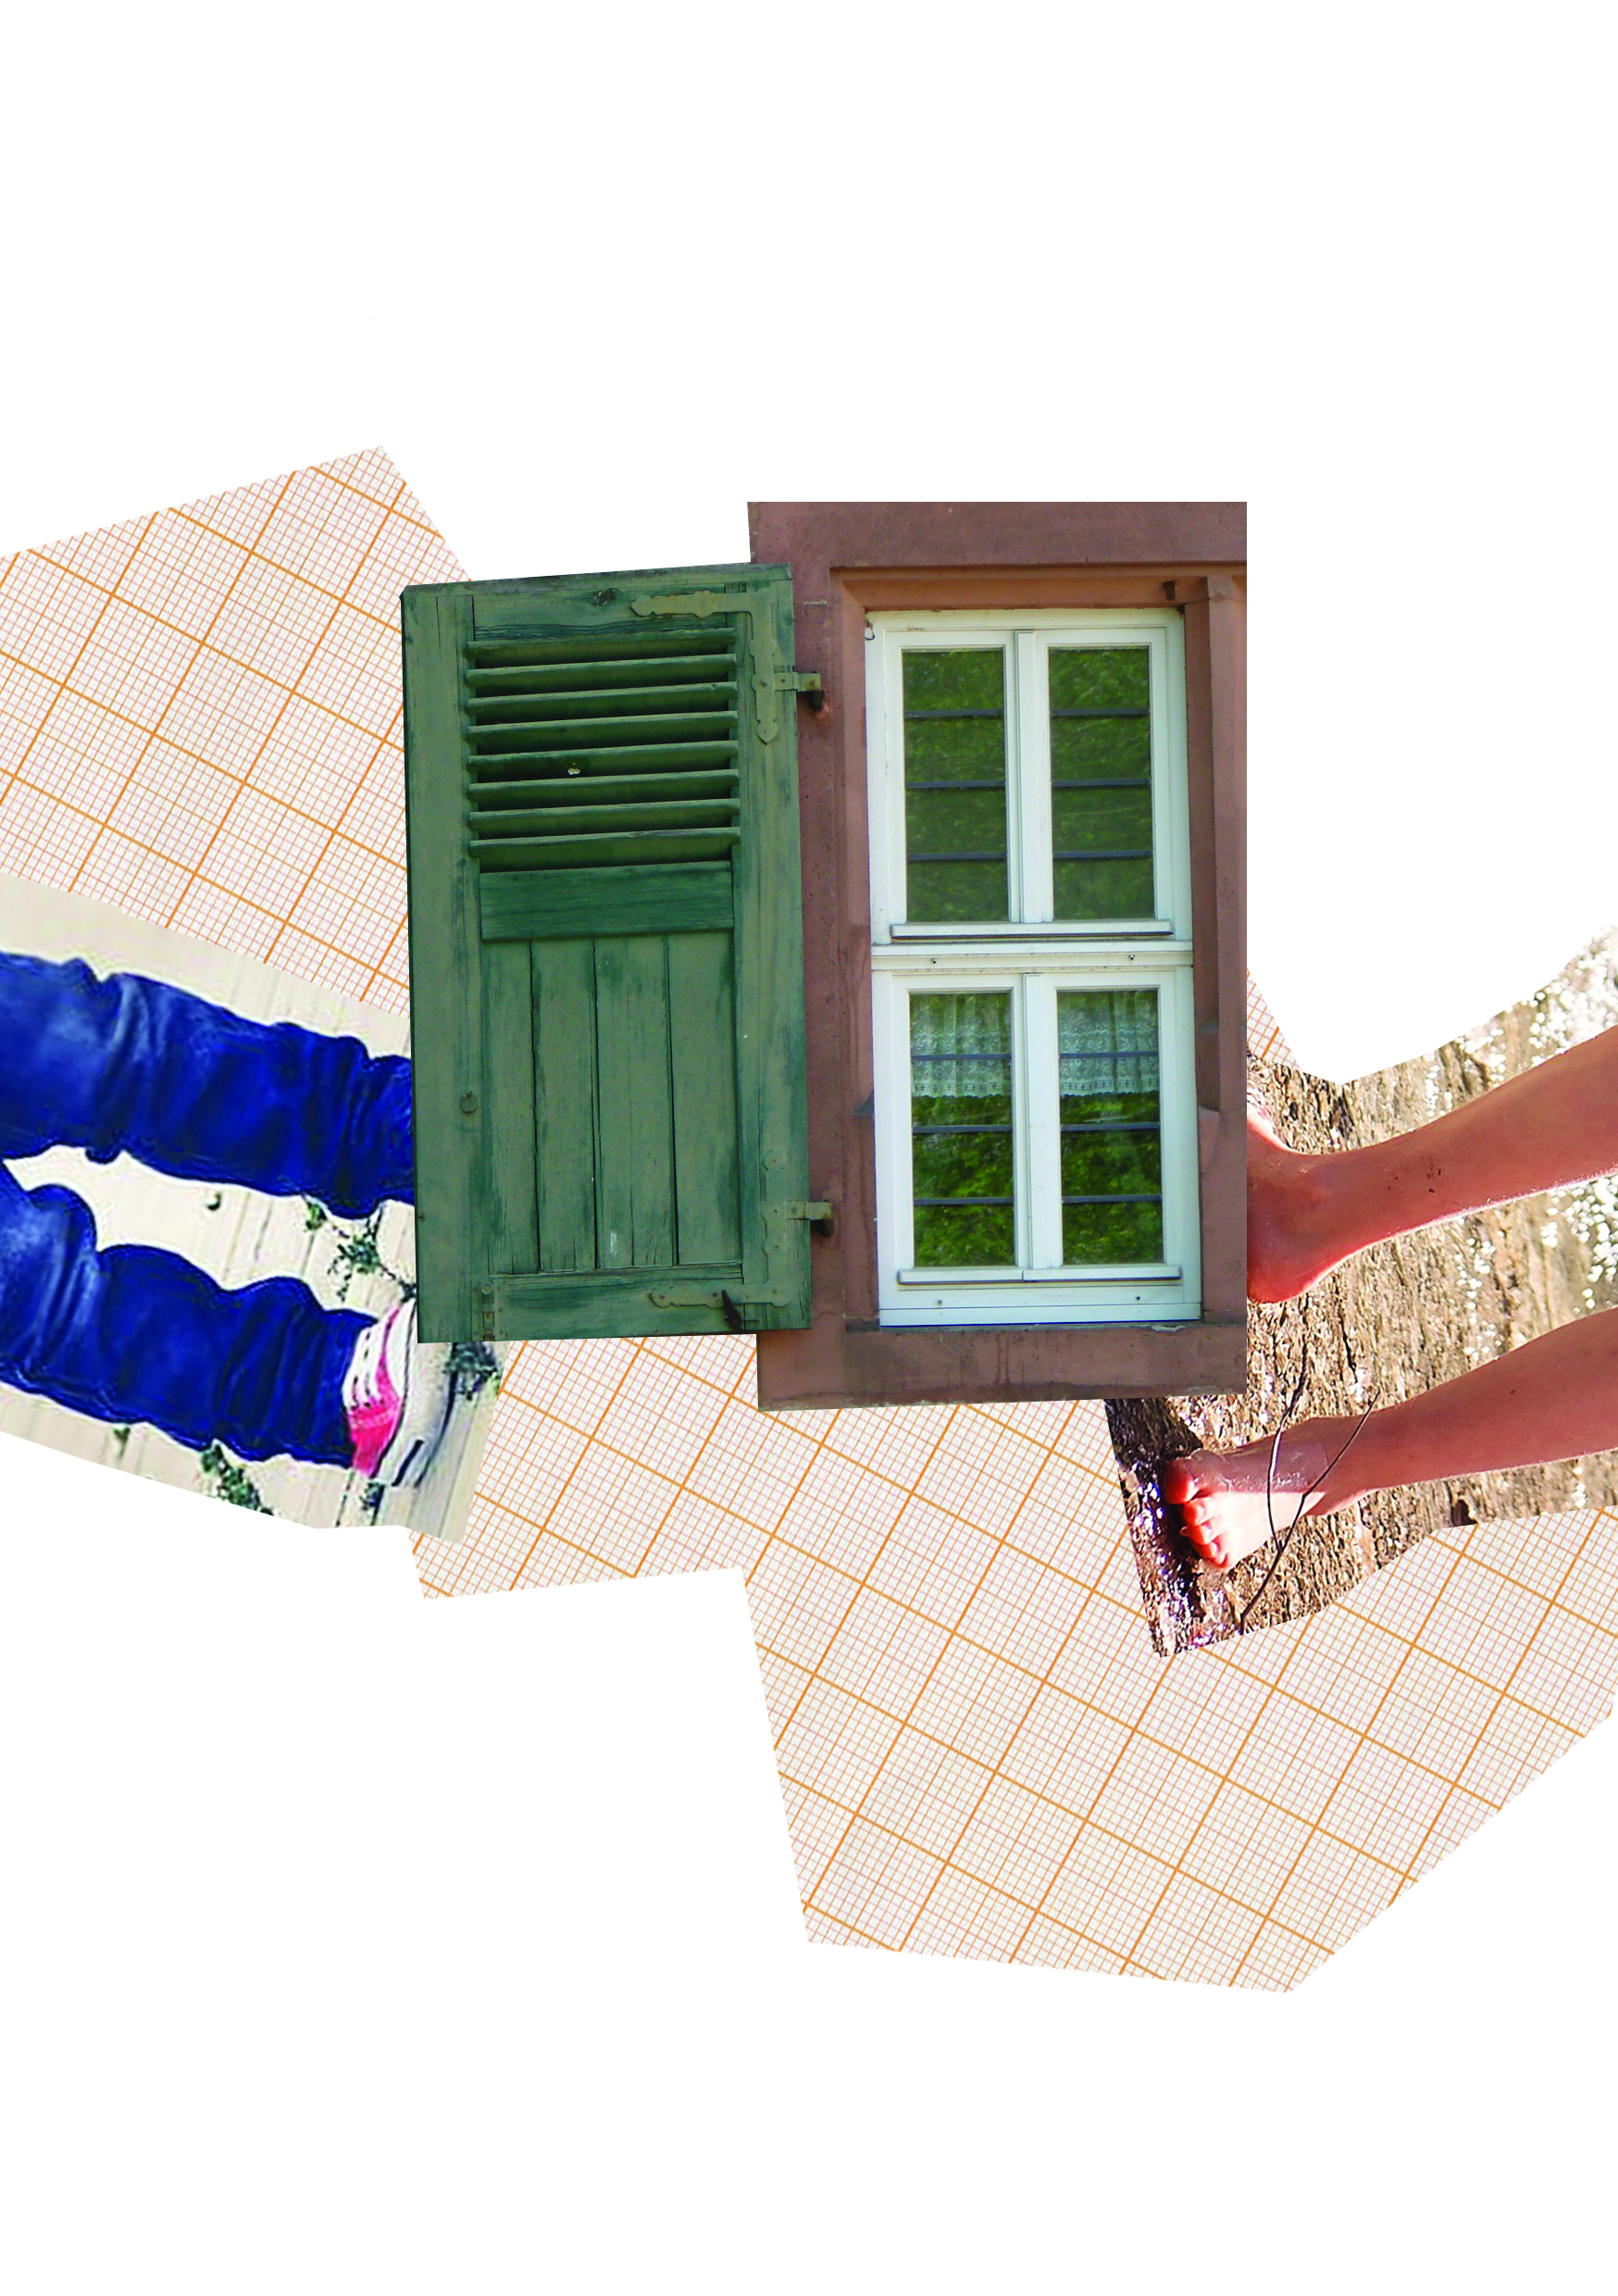
\includegraphics[width=140mm]{../ilustracoes/04_PE.jpg}
\end{figure}
\pagebreak

\chapterspecial{Pé no chão, Vidinha ociosa}{}{Monteiro Lobato}

\noindent{}Fica no extremo da rua o Grupo Escolar, de modo que a meninada passa e
repassa à frente da minha janela. Notei que muitas crianças sofriam dos
pés, pois traziam um no chão e outro calçado. Perguntei a uma delas:

--- Que doença de pés é essa? Bicho arruinado?

O pequeno baixou a cabeça com acanhamento; depois confessou:

--- É ``inconomia''.

Compreendi. Como nos Grupos não se admitem crianças de pé no chão,
inventaram as mães pobres aquela pia fraude. Um pé vai calçado; o outro,
doente de imaginário mal crônico, vai descalço. Um par de botinas dura
assim por dois. Quando o pé de botina em uso fica estragado,
transfere-se a doença de um pé para outro, e o pé de botina de reserva
entra em funções. Destarte, guardadas as conveniências, fica o dispêndio
cortado pelo meio. Acata-se a lei e guarda-se o cobre.

Benditas sejam as mães engenhosas!

\part{Na realidade social}

\pagebreak
\thispagestyle{empty}
\begin{figure}
\vspace*{-.5cm}
\hspace*{-2.3cm}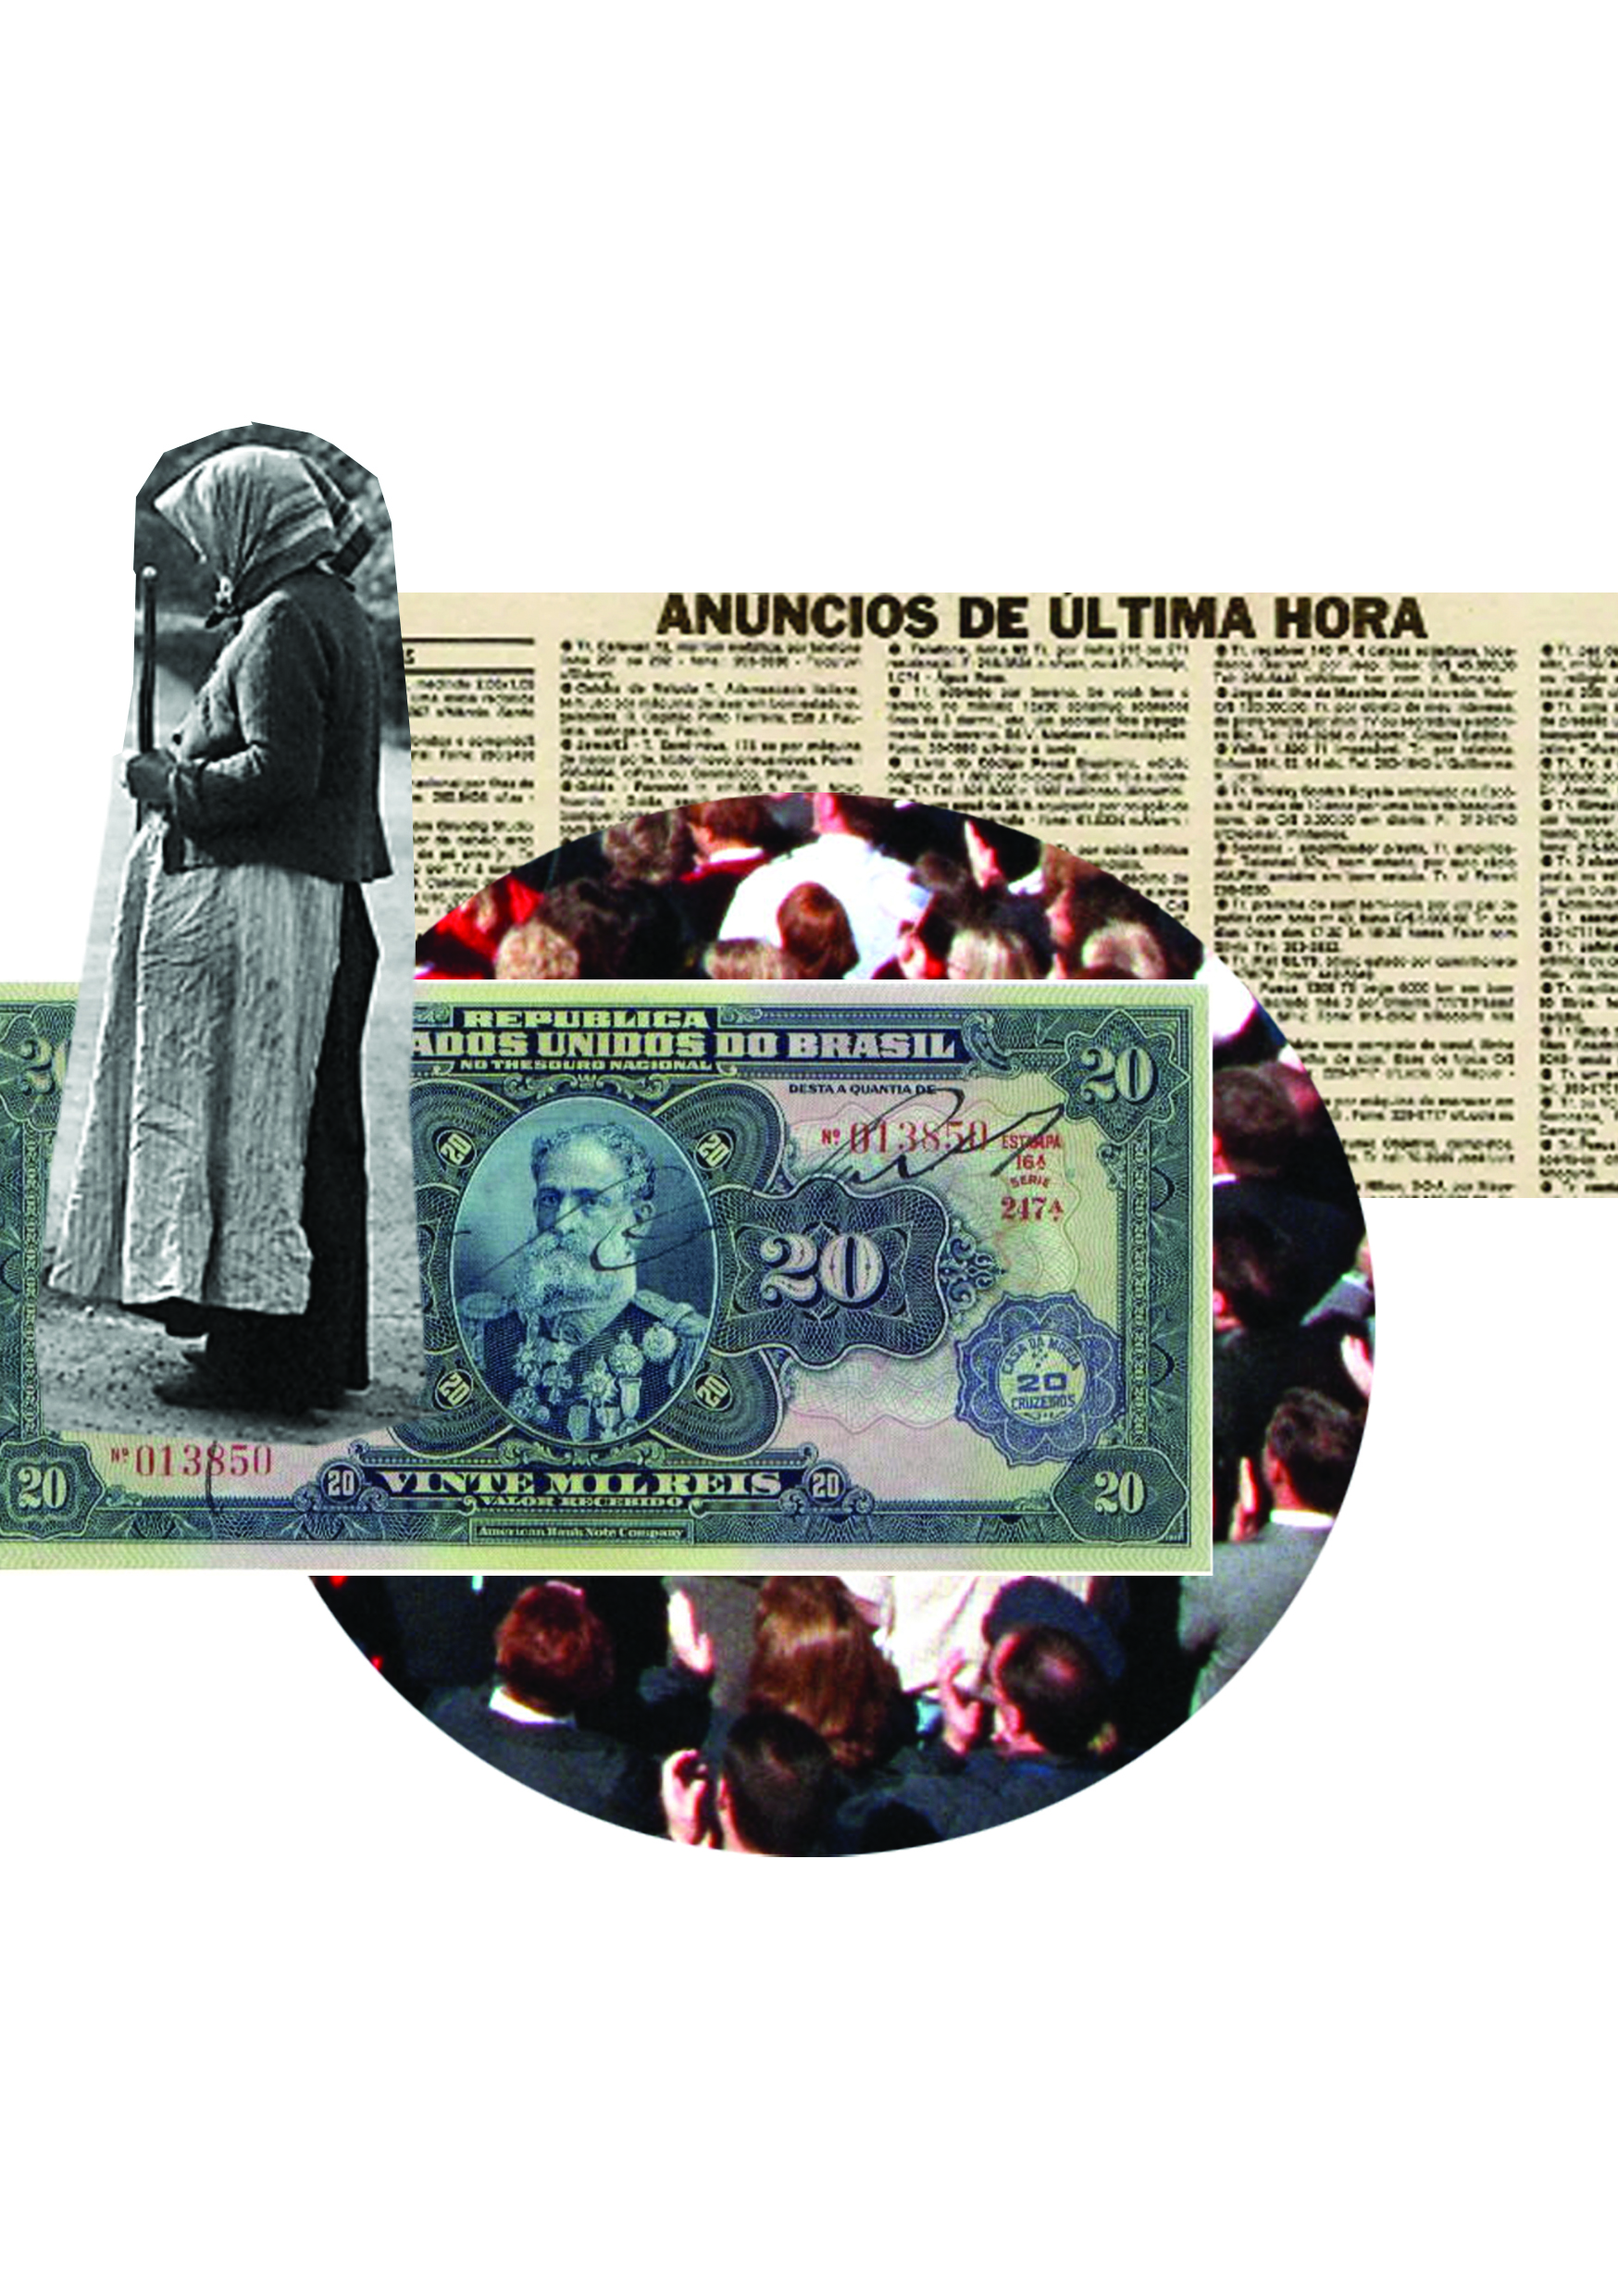
\includegraphics[width=140mm]{../ilustracoes/05_DONA.jpg}
\end{figure}
\pagebreak

\chapterspecial{Dona Expedita}{}{Monteiro Lobato}

--- \ldots{}

--- Minha idade? Trinta e seis\ldots{}

--- Então, venha.

Sempre que dona Expedita se anunciava no jornal, dando um número de
telefone, aquele diálogo se repetia. Seduzidas pelos termos do anúncio,
as donas de casa telefonavam-lhe para ``tratar'' --- e vinha
inevitavelmente a pergunta sobre a idade, com a também inevitável
resposta dos trinta e seis anos. Isso desde antes da Grande Guerra. Veio
o 1914 --- ela continuou nos trinta e seis. Veio a batalha do Marne;
veio o armistício --- ela firme nos trinta e seis. Tratado de Versalhes
--- trinta e seis. Começos de Hitler e Mussolini --- trinta e seis.
Convenção de Munique --- trinta e seis\ldots{}

A futura guerra a reencontrará nos trinta e seis. O mais teimoso dos
empaques! Dona Expedita já está ``pendurada'', escorada de todos os
lados, mas não tem ânimo de abandonar a casa dos trinta e seis anos ---
tão simpática!

E, como só tem trinta e seis anos, veste-se à moda dessa idade, um pouco
mais vistosamente do que a justa medida aconselha. Erro grande! Se à
força de cores claras, ruges e batons, não mantivesse aos olhos do mundo
os seus famosos trinta e seis, era provável que desse a ideia duma bem
aceitável matrona de sessenta\ldots{}

Dona Expedita é ``tia''. Amor só teve um lá pela juventude, do qual às
vezes, nos ``momentos de primavera'', ainda fala. Ah, que lindo moço! Um
príncipe. Passou um dia a cavalo pela sua janela. Passou na tarde
seguinte e ousou um cumprimento. Passou e repassou durante duas semanas
--- e foram duas semanas de cumprimentos e olhares de fogo. E só. Não
passou mais --- desapareceu da cidade para sempre.

O coração da gentil Expedita pulsou intensamente naqueles maravilhosos
quinze dias --- e nunca mais. Nunca mais namorou ou amou ninguém --- por
causa da casmurrice do pai.

Seu pai era um caturra de barbas à Von Tirpitz, português irredutível,
desses que fogem de certos romances de Camilo e reentram na vida. Feroz
contra o sentimentalismo. Não admitia namoros em casa, e nem que se
pronunciasse a palavra casamento. Como vivesse setenta anos, forçou as
duas únicas filhas a se estiolarem ao pé da sua catarreira crônica.
``Filhas são para cuidar da casa e da gente.''\looseness=-1

Morreu, afinal, e arruinado. As duas ``tias'' venderam a casa para
pagamento das contas e tiveram de empregar-se. Sem educação técnica, os
únicos empregos antolhados foram os de criada-grave, dama de companhia
ou ``tomadeira de conta'' --- graus levemente superiores à crua
profissão normal de criada comum. O fato de serem de ``boa família''
autorizava-as ao estacionamento nesse degrau um pouco acima do último.

Um dia a mais velha morreu. Dona Expedita ficou só no mundo. Que fazer,
senão viver? Foi vivendo e especializando-se em lidar com patroas. Por
fim distraía-se com isso. Mudar de emprego era mudar de ambiente --- ver
caras novas, coisas novas, tipos novos. Um cinema --- o seu cinema! O
ordenado, sempre mesquinho. O maior de que se lembrava fora de cento e
cinquenta mil réis. Caiu depois para cento e vinte; depois para cem;
depois oitenta. Inexplicavelmente as patroas iam-lhe diminuindo a paga a
despeito da sua permanência na linda idade dos trinta e seis anos\ldots{}

Dona Expedita colecionava patroas. Teve-as de todos os tipos e naipes
--- das que obrigam as criadas a comprar o açúcar com que adoçam o café
às que voltam para casa de manhã e nunca lançam os olhos sobre o caderno
de compras. Se fosse escritora teria deixado o mais pitoresco dos
livros. Bastava que fixasse metade do que viu e ``padeceu''. O capítulo
das pequeninas decepções seria dos melhores --- como aquele caso dos
quatrocentos mil-réis\ldots{}

Foi certa vez em que, saída de um emprego, andava em procura de outro.
Nessas ocasiões costumava encostar-se à casa de uma família que se dera
com a sua, e lá ficava um mês ou dois até conseguir nova colocação.
Pagava a hospedagem fazendo doces, no que era perita, sobretudo num
certo bolo inglês que mudou de nome, passando a chamar-se o ``bolo de
dona Expedita''. Nesses interregnos comprava todos os dias um jornal
especializado em anúncios domésticos, no qual lia atentamente a seção do
``procura-se''. Com a velha experiência adquirida, adivinhava pela
redação as condições reais do emprego.

--- Porque ``elas'' publicam aqui uma coisa e querem outra --- comentava
filosoficamente, batendo no jornal. --- Para esconder o leite, não há
como as patroas!

E ia lendo, de óculos na ponta do nariz: ``Precisa-se duma senhora de
meia idade para servicinhos leves''.

--- Hum! Quem lê isto pensa que é assim mesmo --- mas não é. O tal
servicinho leve não passa de isca --- é a minhoca do anzol. A mim é que
não me enganam, as biscas\ldots{}

\textls[-10]{Lia todos os ``procura-se'', com um comentário para cada um, até que se
detinha no que lhe cheirava melhor. ``Precisa-se duma senhora de
meia-idade para serviços leves em casa de fino tratamento.''}\looseness=-1

--- Este, quem sabe? Se é casa de fino tratamento, pelo menos fartura há
de haver. Vou telefonar.

E vinha a telefonada do costume com a eterna declaração dos trinta e
seis anos.

O hábito de lidar com patroas manhosas levou-a a lançar mão de vários
recursos estratégicos; um deles: só ``tratar'' pelo telefone e não
dar-se como ela mesma. ``Estou falando em nome duma amiga que procura
emprego.'' Desse modo tinha mais liberdade e jeito de sondar a
``bisca''.

--- ``Essa amiga é uma excelente criatura'' --- e vinham bem dosados
elogios. --- ``Só que não gosta de serviços pesados.''

--- ``Que idade?

--- ``Trinta e seis anos. Senhora de muito boa família --- mas por menos
de cento e cinquenta mil-réis nunca se empregou.

--- ``É muito. Aqui o mais que pagamos é cento e dez --- sendo boa.

--- ``Não sei se ela aceitará. Hei de ver. Mas qual é o serviço?

\textls[-25]{--- ``Leve. Cuidar da casa, fiscalizar a cozinha, espanar --- arrumar\ldots{}}\looseness=-1

--- ``Arrumar? Então é arrumadeira que a senhora quer?''

E dona Expedita pendurava o fone, arrufada, murmurando: ``Outro
ofício!''.

O caso dos quatrocentos mil-réis foi o seguinte. Ela andava sem emprego
e a procurá-lo na seção do ``procura-se''. Súbito, esbarrou com esta
maravilha: ``Precisa-se duma senhora de meia-idade para fazer companhia
a uma enferma; ordenado, quatrocentos mil-réis''.

Dona Expedita esfregou os olhos. Leu outra vez. Não acreditou. Foi em
busca duns óculos novos adquiridos na véspera. Sim. Lá estava escrito
quatrocentos mil-réis!\ldots{}

A possibilidade de apanhar um emprego único no mundo fê-la pular. Correu
a vestir-se, a pôr o chapeuzinho, a avivar as cores do rosto e voou
pelas ruas afora. Foi dar com os costados numa rua humilde; nem rua era
--- numa ``avenida''. Defronte à casa indicada --- casinha de porta e
duas janelas --- havia uma dúzia de pretendentes.\looseness=-1

--- Será possível? O jornal saiu agorinha e já tanta gente por aqui?

Notou que entre as postulantes predominavam senhoras bem-vestidas, com o
aspecto de ``damas envergonhadas''. Natural que assim fosse porque um
emprego de quatrocentos mil-réis era positivamente um fenômeno. Nos
seus\ldots{} trinta e seis anos de vida terrena jamais tivera notícia de
nenhum. Quatrocentos por mês! Que mina! Mas como um emprego assim em
casa tão modesta? ``Já sei. O emprego não é aqui. Aqui é onde se trata
--- casa do jardineiro, com certeza\ldots{}''

Dona Expedita observou que as postulantes entravam de cara risonha e
saíam de cabeça baixa. Evidentemente a decepção da recusa. E o seu
coração batia de gosto ao ver que todas iam sendo recusadas. Quem sabe?
Quem sabe se o destino marcara justamente a ela como a eleita?

Chegou por fim a sua vez. Entrou. Foi recebida por uma velha na cama.
Dona Expedita nem precisou falar. A velha foi logo dizendo:

--- Houve erro no jornal. Mandei por quarenta mil-réis e puseram
quatrocentos\ldots{} Tinha graça eu pagar quatrocentos a uma criada, eu que
vivo à custa do meu filho, sargento da polícia, que nem isso ganha por
mês\ldots{}

Dona Expedita retirou-se com cara exatamente igual à das outras.

O pior da luta entre criados e patroas é que estas são compelidas a
exigir o máximo, e as criadas, por natural defesa, querem o mínimo.
Nunca jamais haverá acordo, porque é choque de totalitarismo com
democracia.

Um dia, entretanto, dona Expedita teve a maior das surpresas: encontrou
uma patroa absolutamente identificada com suas ideias quanto ao ``mínimo
ideal'' --- e, mais que isso, entusiasmada com esse minimalismo --- a
ajudá-la a minimizar o minimalismo!

Foi assim. Dona Expedita estava pela vigésima vez na tal família amiga,
à espera de nova colocação. Lembrou-se de recorrer a uma agência, para a
qual telefonou. ``Quero uma colocação assim, assim, de duzentos
mil-réis, em casa de gente arranjada, fina e, se for possível, em
fazenda. Serviços leves, bom quarto, banho. Aparecendo qualquer coisa
deste gênero, peço que me telefonem'' --- e deu o número do aparelho e
da casa.

Horas depois retinia a campainha do portão.

--- É aqui que mora madame Expedita? --- perguntou em língua atrapalhada
uma senhora alemã, cheia de corpo, de bom aspecto.

A criadinha que atendeu disse que sim, fê-la entrar para o \emph{hall}
de espera e foi correndo avisar dona Expedita. ``Uma estrangeira gorda,
querendo falar com madame!''

--- Que pressa, meu Deus! --- murmurou a solicitada, correndo ao espelho
para os retoques. --- Nem três horas faz que telefonei. Agência boa,
sim\ldots{}

Dona Expedita apareceu no \emph{hall} com um excessozinho de ruge nos
beiços de múmia. Apareceu e conversou --- e maravilhou-se, porque pela
primeira vez na vida encontrava a patroa ideal. A mais \emph{sui
generis} das patroas, de tão integrada no ponto de vista das ``senhoras
de meia-idade que procuram serviços leves''.

O diálogo travou-se num crescendo de animação.

--- Muito boa tarde! --- disse a alemã com a maior cortesia. --- Então
foi madame quem telefonou para a agência?

O ``madame'' causou espécie a dona Expedita.

--- É verdade. Telefonei e dei as condições. A senhora gostou?

--- Muito, mas muito mesmo! Era exatamente o que eu queria. Perfeito.
Mas vim ver pessoalmente, porque o costume é anunciarem uma coisa e a
realidade ser outra.

A observação encantou dona Expedita, cujos olhos brilharam.

--- A senhora parece que está pensando com a minha cabeça. É justamente
isso o que se dá, vivo eu dizendo. As patroas escondem o leite. Anunciam
uma coisa e querem outra. Anunciam serviços leves e botam em cima das
pobres criadas a maior trabalheira que podem. Eu falei, eu insisti com a
agência: servicinhos leves\ldots{}

--- Isso mesmo! --- concordou a alemã, cada vez mais encantada. ---
Serviços leves, bem leves, porque afinal de contas uma criada é gente
--- não é burro de carroça.

--- Claro! Mulheres de certa idade não podem fazer serviços de mocinhas,
como arrumar, lavar, cozinhar quando a cozinheira não vem. Ótimo! Quanto
à acomodação, falei à agência em ``bom quarto''\ldots{}

--- Exatamente! --- concordou a alemã. --- Bom quarto --- com janelas.
Nunca pude conformar-me com isso de as patroas meterem as criadas em
desvãos escuros, sem ar, como se fossem malas. E sem banheiro em que
tomem banho.

Dona Expedita era toda risos e sorrisos. A coisa lhe estava saindo
maravilhosa.

--- E banho quente! --- acrescentou com entusiasmo.

--- Quentíssimo! --- berrou a alemã batendo palmas. --- Isso para mim é
ponto capital. Como pode haver asseio numa casa onde nem banheiro há
para as criadas?

--- Ah, minha senhora, se todas as patroas pensassem assim! --- exclamou
dona Expedita erguendo os olhos para o céu. --- Que felicidade não seria
o mundo! Mas no geral as patroas são más --- e iludem as pobres criadas,
para agarrá-las e explorá-las.

--- Isso mesmo! --- apoiou a alemã. --- A senhora está falando como um
livro de sabedoria. Para cada cem patroas haverá cinco ou seis que
tenham coração --- que compreendam as coisas\ldots{}

--- Se houver! --- duvidou dona Expedita.

O entendimento das duas era perfeito: uma parecia o ``dublê'' da outra.
Debateram o ponto dos ``serviços leves'' com tal mútua compreensão que
os serviços ficaram levíssimos, quase nulos --- e dona Expedita viu
erguer-se diante de si o grande sonho de sua vida: um emprego em que não
fizesse nada, absolutamente nada\ldots{}

--- Quanto ao ordenado --- disse ela (que sempre pedia duzentos para
deixar por oitenta) ---, fixei-o em duzentos\ldots{}

Avançou isso medrosamente e ficou à espera da inevitável repulsa. Mas a
repulsa do costume pela primeira vez não veio. Bem ao contrário disso, a
alemã concordou com entusiasmo.

--- Perfeitamente! Duzentos por mês --- e pagos no último dia de cada
mês.

--- Isso! --- berrou dona Expedita levantando-se da cadeira. --- Ou no
comecinho. Essa história de pagamento em dia incerto nunca foi comigo.
Dinheiro de ordenado é sagrado.

--- Sacratíssimo! --- urrou a alemã levantando-se também.

--- Ótimo --- exclamou dona Expedita. --- Está tudo como eu queria.

--- Sim, ótimo --- repetiu a alemã. --- Mas a senhora também falou em
fazenda\ldots{}

--- Ah, sim, fazenda. Uma fazenda boa, com bastante frutas, bastante
leite, bastante ovos porque há fazendas muito feias.

O quadro da fazenda bonita, toda frutas, leite e ovos, extasiou a alemã.
Que maravilha\ldots{}

Dona Expedita continuou:

--- Gosto muito de lidar com pintinhos.

--- Pintos? Ah, é o maior dos encantos! Adoro os pintos --- as
ninhadas\ldots{} O nosso entendimento vai ser absoluto, madame\ldots{}

O êxtase de ambas sobre a vida de fazenda foi subindo numa vertigem.
Tudo quanto havia de sonhos incubados naquelas almas refloriu viçoso.
Infelizmente a alemã teve a ideia de perguntar:

--- E onde fica a \emph{sua} fazenda, madame?

--- A \emph{minha} fazenda --- repetiu dona Expedita refranzindo a
testa.

--- Sim, a sua fazenda --- a fazenda para onde madame quer que eu vá\ldots{}

--- Fazenda pra onde eu quero que a senhora vá? --- tornou a repetir
dona Expedita, sem entender coisa nenhuma. --- Fazenda, eu? Pois se eu
tivesse fazenda lá andava a procurar emprego?

Foi a vez de a alemã arregalar os olhos, atrapalhadíssima. Também não
estava entendendo coisa nenhuma. Ficou uns instantes no ar. Por fim:

--- Pois madame não telefonou para a agência dizendo que tinha um
emprego assim, assim, na sua fazenda?

--- \emph{Minha} fazenda uma ova! Nunca tive fazenda. Telefonei
procurando emprego, se possível numa fazenda, isso sim\ldots{}

--- Então, então, então\ldots{} --- e a alemã enrubesceu como uma papoula.

--- Pois é --- disse dona Expedita percebendo afinal o
quiproquó.\footnote{quiproquó: confusão; engano, equívoco. Vem da
  expressão latina \emph{quid pro quo}, ``uma coisa pela outra''.} ---
Estamos aqui feito duas idiotas, cada qual querendo emprego e pensando
que a outra é a patroa\ldots{}

O cômico da situação fê-las rirem-se --- e gostosamente, já retomadas à
posição de ``senhoras de meia-idade que procuram serviços leves''.

--- Esta foi muito boa! --- murmurou a alemã levantando-se para sair.
--- Nunca me aconteceu coisa assim. Que agência, hein?

Dona Expedita filosofou.

--- Eu bem que estava desconfiada. A esmola era demais. A senhora ia
concordando com tudo que eu dizia --- até com os banhos quentes! Ora,
isso nunca foi linguagem de patroa --- dessas biscas. A agência errou,
talvez por causa do telefone, que estava danado hoje --- além do que sou
meio dura dos ouvidos\ldots{}

Nada mais havia a dizer. Despediram-se. Depois que a alemã bateu o
portão, dona Expedita fechou a porta, com um suspiro arrancado do fundo
das tripas.

--- Que pena, meu Deus! Que pena não existirem no mundo patroas que
pensem como as criadas\ldots{}

\blankpage

\pagebreak
\thispagestyle{empty}
\begin{figure}
\vspace*{-.5cm}
\hspace*{-2.3cm}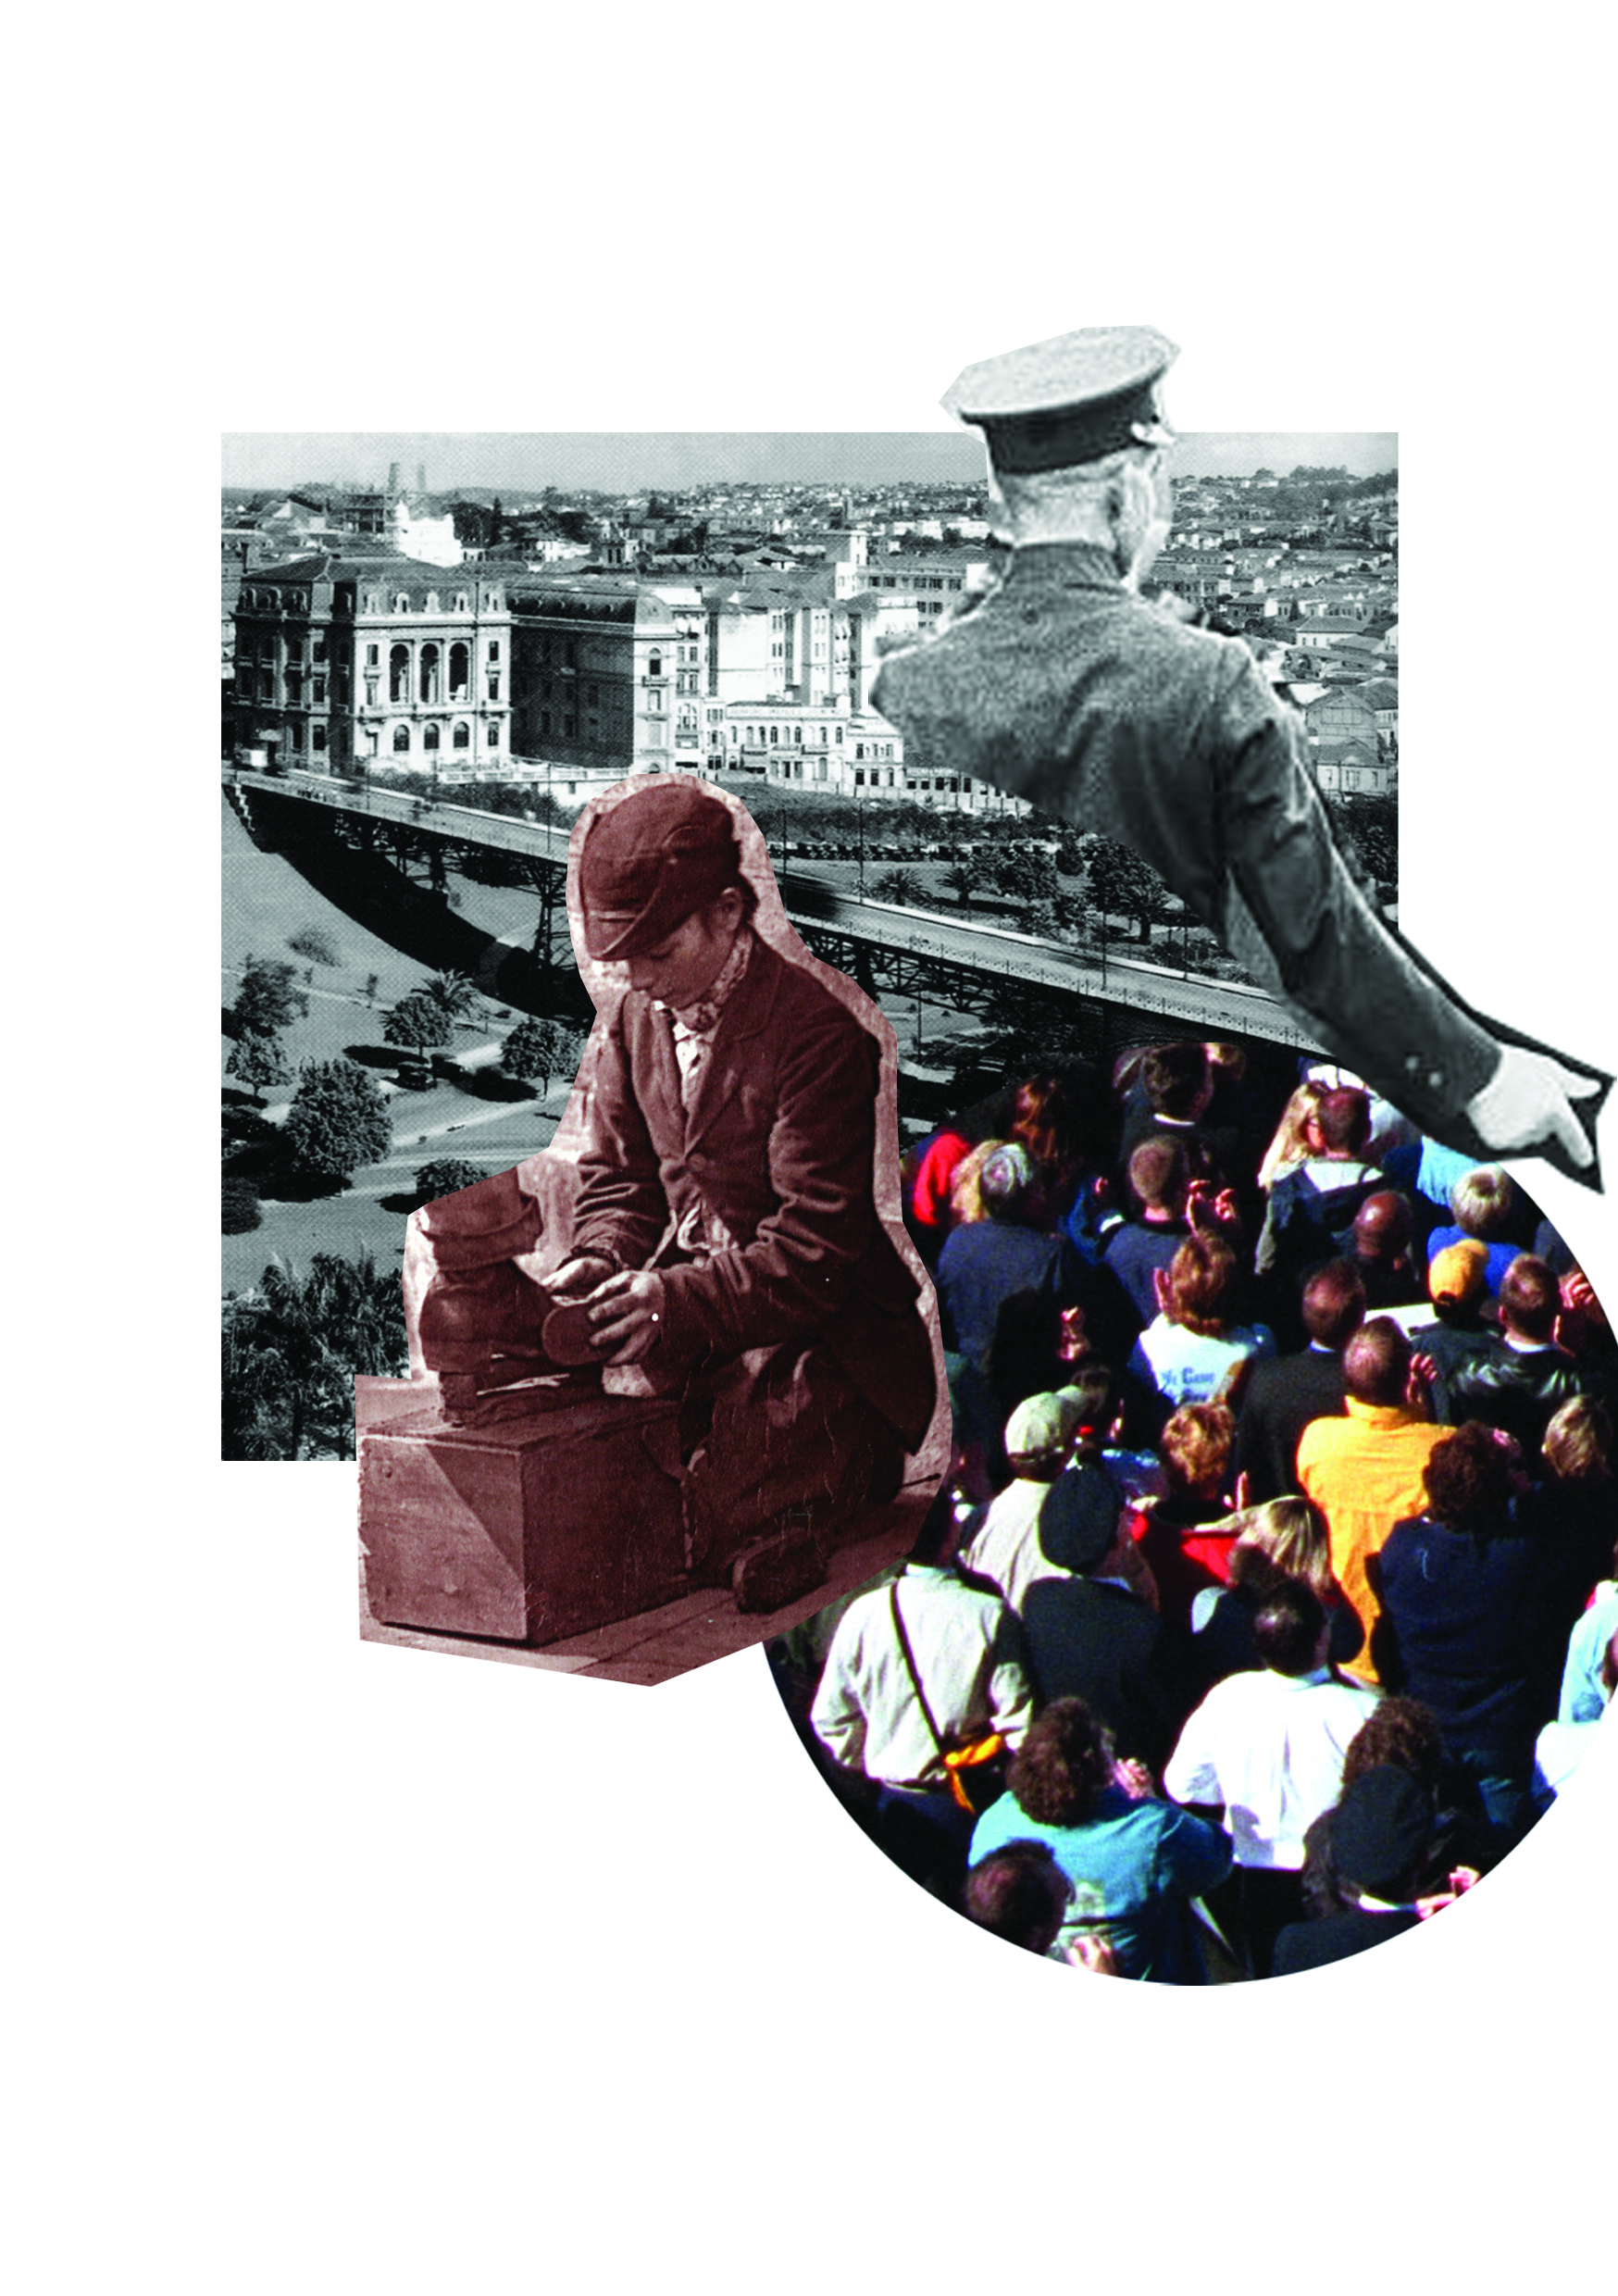
\includegraphics[width=140mm]{../ilustracoes/06_FISCO.jpg}
\end{figure}
\pagebreak

\chapterspecial{O fisco}{(Conto de Natal)}{Monteiro Lobato}

\section{Prólogo}

No princípio era o pântano, com valas de agrião e rãs coaxantes. Hoje é
o parque do Anhangabaú, todo ele relvado, com ruas de asfalto, pérgola
grata a namoriscos noturnos, a Eva de Brecheret, a estátua dum
adolescente nu que corre --- e mais coisas. Autos voam pela via central,
e cruzam-se pedestres em todas as direções. Lindo parque,
civilizadíssimo.

Atravessando-o certa tarde, vi formar-se ali um bolo de gente, rumo ao
qual vinha vindo um polícia apressado.

``\emph{Fagocitose}'', pensei. A rua é a artéria; os passantes, o
sangue. O desordeiro, o bêbado, o gatuno são os micróbios maléficos,
perturbadores do ritmo circulatório. O soldado de polícia é o glóbulo
branco --- o \emph{fagócito} de Metchnikoff.

Está de ordinário parado no seu posto, circunvagando olhares atentos.
Mal se congestiona o tráfego pela ação antissocial do desordeiro, o
fagócito move-se, caminha, corre, cai a fundo sobre o mau elemento e
arrasta-o para o xadrez.

Foi assim naquele dia.

Dia sujo, azedo. Céu dúbio, de decalcomania vista pelo avesso. Ar
arrepiado.

Alguém perturbara a paz do jardim, e em redor desse rebelde logo se
juntou um grupo de glóbulos vermelhos, vulgo passantes. E lá vinha agora
o fagócito fardado restabelecer a harmonia universal.

O caso girava em torno de uma criança maltrapilha, que tinha a tiracolo
uma caixa tosca de engraxate, visivelmente feita pelas suas próprias
mãos. Muito sarapantado, com lágrimas a brilharem nos olhos cheios de
pavor, o pequeno murmurava coisas de ninguém atendidas. Sustinha-o pela
gola um fiscal da Câmara.

--- Então, seu cachorrinho, sem licença, hein? --- exclamava entre
colérico e vitorioso o mastim municipal, focinho muito nosso conhecido.
É um que não é um mas sim legião, e sabe ser tigre ou cordeiro conforme
o naipe do contraventor.

A miserável criança evidentemente não entendia, não sabia que coisa era
aquela de licença, tão importante, reclamada assim a empuxões brutais.
Foi quando entrou em cena o polícia.

Este glóbulo branco era preto. Tinha beiço de sobejar e nariz invasor de
meia cara, aberto em duas ventas acesas, relembrativas das cavernas de
Trofônio. Aproximou-se e rompeu o magote com um napoleônico
``Espalha!''.

Humildes alas se abriram àquele Sésamo, e a Autoridade, avançando,
interpelou o Fisco:

--- Que encrenca é esta, chefe?

--- Pois este cachorrinho não é que está exercendo ilegalmente a
profissão de engraxate? Encontrei-o banzando por aqui com estes troços,
a fisgar com os olhos os pés dos transeuntes e a dizer ``Engraxa,
freguês''. Eu vi a coisa de longe.

Vim pé ante pé, disfarçando e, de repente, \emph{nhoc}! ``Mostre a
licença'', gritei. ``Que licença?'', perguntou ele com arzinho de
inocência. ``Ah, você diz que licença, cachorro? Está me debochando,
ladrão? Espera que te ensino o que é licença, trapo!'' E agarrei-o. Não
quer pagar a multa. Vou levá-lo ao depósito, autuar a infração para
proceder de acordo com as posturas --- concluiu com soberbo entono o
cariado canino da Maxila Fiscal.

O solene Mata-Piolho da Manopla Policial concordou.

--- É isso mesmo. Casca-lhes!

E chiando por entre os dentes uma cusparada de esguicho, deu a sua
sacudidela suplementar no menino. Depois voltou-se para os basbaques e
ordenou com império de soba africano:

--- Circula, paisanada! É ``purivido'' ajuntamentos de mais de um.

Os glóbulos vermelhos dispersaram-se em silêncio. O buldogue lá seguiu
com o pequeno nas unhas. E o Pau de Fumo, em atitude de Bonaparte em
face das pirâmides, ficou, de dedo no nariz e boca entreaberta, a gozar
a prontidão com que, num ápice, sua energia resolvera o tumor maligno
formado na artéria sob a sua fiscalização.

\section{O Brás}

Também lá, no princípio, era o charco --- terra negra, fofa, turfa
tressuante, sem outra vegetação além dessas plantinhas miseráveis que
sugam o lodo como minhocas. Aquém da várzea, na terra firme e alta, São
Paulo crescia. Erguiam-se casas nos cabeços, e esgueiravam-se ladeiras
encostas abaixo: a Boa Morte, o Carmo, o Piques; e ruas, Imperador,
Direita, São Bento. Poetas cantavam-lhe as graças nascentes:

\emph{Ó Liberdade, ó Ponte Grande, ó Glória\ldots{}}

Deram-lhe um dia o Viaduto do Chá, esse arrojo\ldots{} Os paulistanos pagavam
sessenta réis para, ao atravessá-lo, conhecerem a vertigem dos abismos.
E em casa narravam a aventura às esposas e mães, pálidas de espanto. Que
arrojo de homem, o Jules Martin, que construíra aquilo!

Enquanto São Paulo crescia o Brás coaxava. Enluravam-se naquele brejal
legiões de sapos e rãs. À noite, do escuro da terra um coral subia de
coaxos, \emph{panpans} de ferreiro, latidos de mimbuias, \emph{glu-glus}
de untanhas; e por cima, no escuro do ar, vaga-lumes ziguezagueantes
riscavam fósforos às tontas.

E assim foi até o dia da avalanche italiana.

Quando lá no Oeste a terra roxa se revelou mina de ouro das que pagam
duzentos por um, a Itália vazou para cá a espuma da sua transbordante
taça de vida. E São Paulo, não bastando ao abrigo da nova gente,
assistiu, atônito, ao surto do Brás.

Drenos sangraram em todos os rumos o brejal turfoso; a água escorreu; os
espavoridos sapos sumiram-se aos pulos para as baixadas do Tietê; rã
comestível não ficou uma para memória da raça; e, breve, em substituição
aos guembês, ressurtiu a cogumelagem de centenas e centenas de casinhas
típicas --- porta, duas janelas e platibanda.

Numerosas ruas, alinhadas na terra cor de ardósia que já o sol
ressequira e o vento erguia em nuvens de pó negro, margearam-se com
febril rapidez desses prediozinhos térreos, iguais uns aos outros, como
saídos do mesmo molde, pífios, mas únicos possíveis então. Casotas
provisórias, desbravadoras da lama e vencedoras do pó à força de preço
módico.

E o Brás cresceu, espraiou-se de todos os lados, comeu todo o barro
preto da Mooca, bateu estacas no Marco da Meia Légua, lançou-se rumo à
Penha, pôs de pé igrejas, macadamizou ruas, inçou-se de fábricas, viu
surgirem avenidas e vida própria, e cinemas, e o Colombo, e o namoro, e
o corso pelo Carnaval. E lá está hoje enorme, feito a cidade do Brás,
separado de São Paulo pelo faixão vermelho da Várzea aterrada --- Pest
da Buda à beira do Tamanduateí plantada.

São duas cidades vizinhas, distintas de costumes e de almas já bem
diversas.

Ir ao Brás é uma viagem. O Brás não é ali, como o Ipiranga; é lá do
outro lado, embora mais perto que o Ipiranga. Diz-se vou ao Brás como
quem diz vou à Itália. Uma Itália agregada como um bócio recente e
autônomo a uma \emph{urbs} antiga, filha do país; uma Itália função da
terra negra, italiana por sete décimos e \emph{algo nuevo} pelos
restantes.

O Brás trabalha de dia e à noite gesta. Aos domingos fandanga ao som do
bandolim. Nos dias de festa nacional (destes tem predileção pelo 21 de
Abril: vagamente o Brás desconfia que o barbeiro da Inconfidência,
porque barbeiro, havia de ser um patrício), nos dias feriados o Brás vem
a São Paulo. Entope os bondes no travessio da Várzea e cá ensardinha-se
nos autos: o pai, a mãe, a sogra, o genro e a filha casada no banco de
trás; o tio, a cunhada, o sobrinho e o Pepino escoteiro no da frente;
filhos miúdos por entremeio; filhos mais taludos ao lado do motorista;
filhos engatinhantes debaixo dos bancos; filhos em estado fetal no
ventre bojudo das matronas. Vergado de molas, o carro geme sob a carga e
arrasta-se a meia velocidade, exibindo a Pauliceia aos olhos arregalados
daquele exuberante cacho humano.

Finda a corrida, o auto debulha-se do enxame no Triângulo e o bando toma
de assalto as confeitarias para um regabofe de \emph{spumones}, gasosas,
croquetes. E tão a sério toma a tarefa que ali pelas nove horas não
restam iscas de empada nos armários térmicos, nem vestígios de sorvete
no fundo das geladeiras. O Brás devora tudo, ruidosa, alegremente, e com
massagens ajeitadoras do abdômen sai impando bem-aventurança estomacal.
Caroços de azeitonas, palitos de camarões, guardanapos de papel, pratos
de papelão seguem nas munhecas da petizada como lembrança da festa e
consolo ao bersalherzinho que lá ficou de castigo em casa, berrando com
goela de Caruso.

Em seguida, toca para o cinema! O Brás abarrota os de sessão corrida. O
Brás chora nos lances lacrimogêneos da Bertini e ri nas comédias a gás
hilariante da L-Ko mais do que autorizam os mil e cem da entrada. E
repete a sessão, piscando o olho: é o jeito de dobrar a festa em
extensão e obtê-la a meio preço --- quinhentos e cinquenta réis, uma
pechincha.

As mulheres do Brás, ricas de ovário, são vigorosíssimas de útero.
Desovam quase filho e meio por ano, sem interrupção, até que se acabe a
corda ou rebente alguma peça essencial da gestatória.

É de vê-las na rua. Bojudas de seis meses, trazem um Pepininho à mão e
um choramingas à mama. À tarde o Brás inteiro chia de criançalha a
chutar bolas de pano, a jogar pião, ou a piorra, ou o tento de telha, ou
o tabefe, com palavreados mistos de português e dialetos de Itália.
Mulheres escarranchadas às portas, com as mãos ocupadas em manobras de
agulha de osso, espigaitam para os maridos os sucessos do dia, que eles
ouvem filosoficamente, cachimbando calados ou cofiando a bigodeira à
Humberto Primo.

De manhã esfervilha o Brás de gente estremunhada a caminho das fábricas.

A mesma gente reflui à tarde aos magotes --- homens e mulheres de cesta
no braço, ou garrafas de café vazias penduradas do dedo; meninas,
rapazes, raparigotas de pouco seio, galantes, tagarelas, com o namoro
rente.

Desce a noite, e nos desvãos de rua, nos becos, nas sombras, o amor
lateja. Ciciam vozes cautelosas das janelas para os passeios; pares em
conversa disfarçada nos portões emudecem quando passa alguém ou tosse lá
dentro o pai.

Durante o escuro das fitas, nos cinemas, há contatos, longos,
febricitantes; e quando nos intervalos irrompe a luz, não sabem os
namorados o que se passou na tela --- mas estão de olhos langues, em
quebreira de amor.

É o latejar da messe futura. Todo aquele eretismo por música, com cicios
de pensamentos de cartão-postal, estará morto no ano seguinte ---
legalizado pela Igreja e pelo juiz, transfeita a sua poesia em choro de
criança e nas trabalheiras sem-fim da casa humilde.

Tal menina rosada, leve de andar, toda requebros e dengues, que passa na
rua vestida com graça e atrai os olhares gulosos dos homens, não a
reconhecereis dois anos depois na lambona filhenta que deblatera com o
verdureiro a propósito do feixe de cenouras em que há uma menor que as
outras.

Filho da lama negra, o Brás é como ela um sedimento de aluvião. É São
Paulo, mas não é a Pauliceia. Ligados pela expansão urbana, separa-os
uma barreira. O velho caso do fidalgo e do peão enriquecido.

\section{Pedrinho, sem ser consultado, nasce}

Viram-se, ele e ela. Namoraram-se. Casaram.

Casados, proliferaram. Eram dois. O amor transformou-os em três. Depois
em quatro, em cinco, em seis\ldots{}

Chamava-se Pedrinho o filho mais velho.

\section{A vida}

De pé na porta a mãe espera o menino que foi à padaria. Entra o pequeno
com as mãos abanando.

--- Diz que subiu; custa agora oitocentos.

A mulher, com uma criança ao peito, franze a testa desconsolada.

--- Meu Deus! Onde iremos parar? Ontem era a lenha; hoje é o pão\ldots{} Tudo
sobe. Roupa, pela hora da morte. José ganhando sempre a mesma coisa. Que
será de nós, Deus do céu!

E voltando-se para o filho:

--- Vá a outra padaria, quem sabe se lá\ldots{} Se for a mesma coisa, traga
só um pedaço.

Pedrinho sai. Nove anos. Franzino, doentio, sempre mal alimentado e
vestido com os restos das roupas do pai.

Trabalha este num moinho de trigo, ganhando jornal insuficiente para a
manutenção da família. Se não fosse a bravura da mulher, que lavava para
fora, não se sabe como poderiam subsistir. Todas as tentativas feitas
com o intuito de melhorarem a vida com indústrias caseiras esbarraram no
óbice tremendo do Fisco. A fera condenava-os à fome. Assim escravizados,
José perdeu aos poucos a coragem, o gosto de viver, a alegria. Vegetava,
recorrendo ao álcool para alívio de uma situação sem remédio.

Bendito sejas, amável veneno, refúgio derradeiro do miserável, gole
inebriante de morte que faz esquecer a vida e lhe resume o curso!
Bendito sejas!

Apesar de moça, vinte e sete apenas, Mariana aparentava o dobro. A
labuta permanente, os partos sucessivos, a chiadeira da filharada, a
canseira sem-fim, o serviço emendado com o serviço, sem folga outra além
da que o sono força, fizeram da bonita moça que fora a escanzelada besta
de carga que era.

Seus dez anos de casada\ldots{} Que eternidade de canseiras!\ldots{}

Rumor à porta. Entra o marido. A mulher, ninando a pequena de peito,
recebe-o com a má nova.

--- O pão subiu, sabe?

Sem murmurar palavra o homem senta-se, apoiando nas mãos a cabeça.

Está cansado.

A mulher prossegue:

--- Oitocentos réis o quilo agora. Ontem foi a lenha; hoje é o pão\ldots{} E
lá?

Sempre aumentaram o jornal?

O marido esboçou um gesto de desalento e permaneceu mudo, com o olhar
vago. A vida era um jogo de engrenagens de aço entre cujos dentes se
sentia esmagar. Inútil resistir. Destino, sorte.

Na cama, à noite, confabulavam. A mesma conversa de sempre. José acabava
grunhindo rugidos surdos de revolta. Falava em revolução, saque. A
esposa consolava-o, de esperança posta nos filhos.

--- Pedrinho tem nove anos. Logo estará em ponto de ajudar-nos. Um pouco
mais de paciência e a vida melhora.

Aconteceu que nessa noite Pedrinho ouviu a conversa e a referência à sua
futura ação. Entrou a sonhar. Que fariam dele? Na fábrica, como o pai?
Se lhe dessem a escolher, iria a engraxador. Tinha um tio no ofício, e
em casa do tio era menor a miséria. Pingavam níqueis.

Sonho vai, sonho vem, brota na cabeça do menino uma ideia, que cresceu,
tomou vulto extraordinário e fê-lo perder o sono. Começar já, amanhã,
por que não? Faria ele mesmo a caixa; escovas e graxa, com o tio
arranjaria. Tudo às ocultas, para surpresa dos pais! Iria postar-se num
ponto por onde passasse muita gente. Diria como os outros: ``Engraxa,
freguês!'', e níqueis haviam de juntar-se no seu bolso. Voltaria para
casa recheado, bem tarde, com ar de quem as fez\ldots{} E mal a mãe começasse
a ralhar, ele lhe taparia a boca despejando na mesa o monte de dinheiro.
O espanto dela, a cara admirada do pai, o regalo da criançada com a
perspectiva da ração em dobro! E a mãe a apontá-lo aos vizinhos: ``Estão
vendo que coisa? Ganhou, só ontem, primeiro dia, dois mil-réis!''. E a
notícia a correr\ldots{} E murmúrios na rua quando o vissem passar: ``É
aquele!''.

Pedrinho não dormiu essa noite. De manhãzinha já estava a dispor a
madeira dum caixote velho sob forma de caixa de engraxate ao molde
clássico. Lá a fez.

Os pregos, bateu com o salto de uma velha botina. As tábuas, serrou
pacientemente com um facão dentado. Saiu coisa tosca e mal-ajambrada, de
fazer rir a qualquer carapina e pequena demais --- sobre ela só caberia
um pé de criança igual ao seu. Mas Pedrinho não notou nada disso, e
nunca trabalho nenhum de carpintaria lhe pareceu mais perfeito.

Conclusa a caixa, pô-la a tiracolo e esgueirou-se para a rua, às
escondidas. Foi à casa do tio e lá obteve duas velhas escovas fora de
uso, já sem pelos, mas que à sua exaltada imaginação se afiguraram
ótimas. Graxa, conseguiu alguma raspando o fundo de quanta lata velha
encontrou no quintal.

Aquele momento marcou em sua vida um apogeu de felicidade vitoriosa. Era
como um sonho --- e sonhando saiu para a rua. Em caminho viu o dinheiro
crescer-lhe nas mãos, aos montes. Dava à família parte, e o resto
encafuava.

Quando enchesse o canto da arca onde tinha suas roupas, montaria um
``corredor'', pondo a jornal outros colegas. Aumentaria as rendas!
Enriqueceria! Compraria bicicletas, automóvel, doces todas as tardes na
confeitaria, livros de figura, uma casa, um palácio, outro palácio para
os pais. Depois\ldots{}

Chegou ao parque. Tão bonito aquilo --- a relva tão verde, tosadinha\ldots{}
Havia de ser bom o ponto. Parou perto de um banco de pedra e, sempre
sonhando as futuras grandezas, pôs-se a murmurar para cada passante,
fisgando-lhe os pés:

--- Engraxa, freguês!

Os fregueses passavam sem lhe dar atenção. ``É assim mesmo'', refletia
consigo o menino; ``no começo custa. Depois se afreguesam.''

Súbito, viu um homem de boné caminhando para o seu lado. Olhou-lhe para
as botinas. Sujas. Viria engraxar, com certeza --- e o coração bateu-lhe
apressado, no tumulto delicioso da estreia. Encarou o homem já a cinco
passos e sorriu com infinita ternura nos olhos, num agradecimento
antecipado em que havia tesouros de gratidão.

Mas em vez de lhe espichar o pé, o homem rosnou aquela terrível
interpelação inicial:

--- Então, cachorrinho, que é da licença?

\section{Epílogo? Não! Primeiro ato\ldots{}}

Horas depois o fiscal aparecia em casa de Pedrinho com o pequeno pelo
braço.

Bateu. O pai estava, mas quem abriu foi a mãe. O homem nesses momentos
não aparecia, para evitar explosões. Ficou a ouvir do quarto o
bate-boca.

O fiscal exigia o pagamento da multa. A mulher debateu-se, arrepelou-se.
Por fim, rompeu em choro.

--- Não venha com lamúrias --- rosnou o buldogue ---; conheço o truque
dessa aguinha nos olhos. Não me embaça, não. Ou bate aqui os vinte
mil-réis, ou penhoro toda esta cacaria. Exercer ilegalmente a profissão!
Ora dá-se! E olhe cá, madama, considere-se feliz de serem só vinte. Eu é
de dó de vocês, uns miseráveis; senão, aplicava o máximo. Mas se resiste
dobro a dose!

A mulher limpou as lágrimas. Seus olhos endureceram, com uma chispa má
de ódio represado a faiscar. O Fisco, percebendo-o, motejou:

--- Isso. É assim que as quero --- tesinhas, ah, ah.

Mariana nada mais disse. Foi à arca, reuniu o dinheiro existente ---
dezoito mil-réis ratinhados havia meses, aos vinténs, para o caso
dalguma doença, e entregou-os ao Fisco.

--- É o que há --- murmurou com tremura na voz.

O homem pegou o dinheiro e gostosamente o afundou no bolso, dizendo:

--- Sou generoso, perdoo o resto. Adeusinho, amor!

E foi à venda próxima beber dezoito mil-réis de cerveja.

Enquanto isso, no fundo do quintal, o pai batia furiosamente no menino.

\blankpage

\pagebreak
\thispagestyle{empty}
\begin{figure}
\vspace*{-.5cm}
\hspace*{-2.3cm}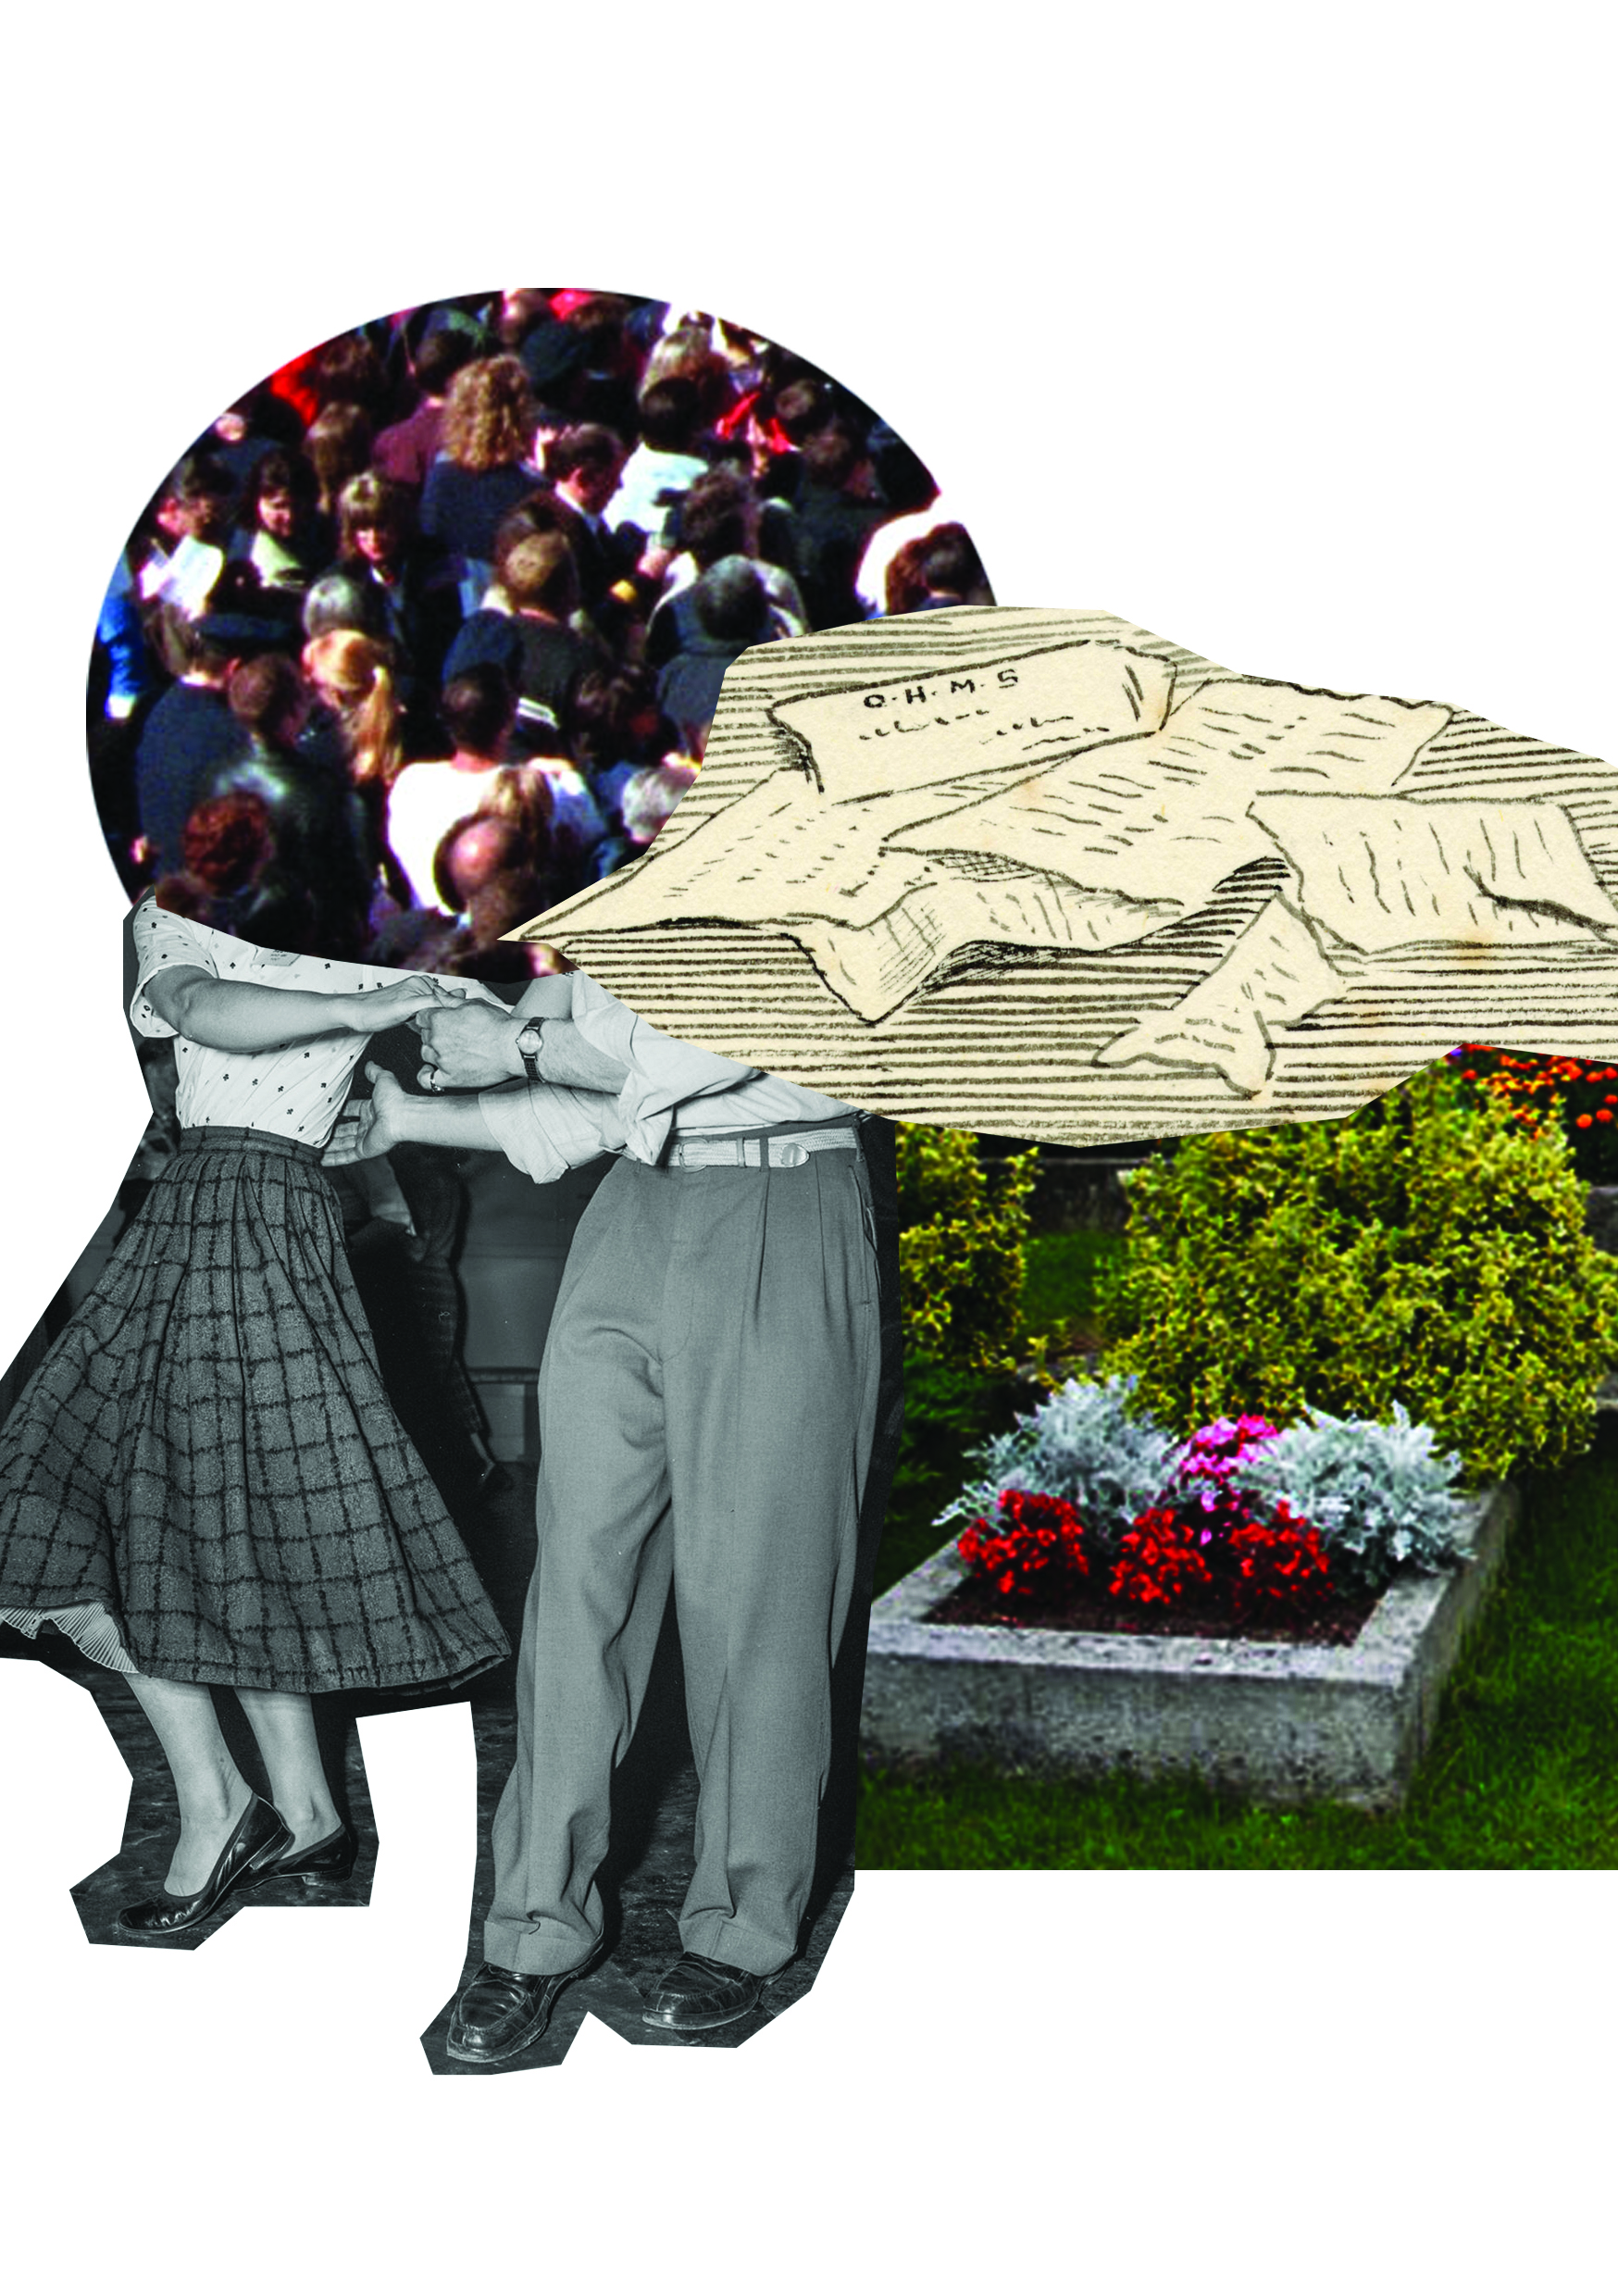
\includegraphics[width=140mm]{../ilustracoes/07_GALERIA.jpg}
\end{figure}
\pagebreak

\chapterspecial{Galeria póstuma}{}{Machado de Assis}

\section{Capítulo primeiro}

Não, não se descreve a consternação que produziu em todo o Engenho
Velho, e particularmente no coração dos amigos, a morte de Joaquim
Fidélis. Nada mais inesperado. Era robusto, tinha saúde de ferro, e
ainda na véspera fora a um baile, onde todos o viram conversado e
alegre. Chegou a dançar, a pedido de uma senhora sexagenária, viúva de
um amigo dele, que lhe tomou do braço, e lhe disse:

--- Venha cá, venha cá, vamos mostrar a estes criançolas como é que os
velhos são capazes de desbancar tudo.

Joaquim Fidélis protestou sorrindo; mas obedeceu e dançou. Eram duas
horas quando saiu, embrulhando os seus sessenta anos numa capa grossa
--- estávamos em junho de 1879 ---, metendo a calva na carapuça,
acendendo um charuto e entrando lepidamente no carro.

No carro é possível que cochilasse; mas, em casa, malgrado a hora e o
grande peso das pálpebras, ainda foi à secretária, abriu uma gaveta,
tirou um de muitos folhetos manuscritos --- e escreveu durante três ou
quatro minutos umas dez ou onze linhas. As últimas palavras eram estas:
``Em suma, baile chinfrim; uma velha gaiteira obrigou-me a dançar uma
quadrilha; à porta um crioulo pediu-me as festas. Chinfrim!''. Guardou o
folheto, despiu-se, meteu-se na cama, dormiu e morreu.

Sim, a notícia consternou a todo o bairro. Tão amado que ele era, com os
modos bonitos que tinha, sabendo conversar com toda a gente, instruído
com os instruídos, ignorante com os ignorantes, rapaz com os rapazes, e
até moça com as moças. E depois, muito serviçal, pronto a escrever
cartas, a falar a amigos, a concertar brigas, a emprestar dinheiro. Em
casa dele reuniam-se à noite alguns íntimos da vizinhança, e às vezes de
outros bairros; jogavam o voltarete\footnote{voltarete: jogo de baralho
  com quarenta cartas e três parceiros; cada um recebe nove cartas,
  restando treze na mesa para compras.} ou o \emph{whist},\footnote{\emph{whist},
  uíste: jogo de baralho comum nos séculos \textsc{xviii} e \textsc{xix}, ancestral do
  \emph{bridge}, disputado com 52 cartas, divididas equitativamente por
  quatro jogadores em duas parcerias.} falavam de política. Joaquim
Fidélis tinha sido deputado até à dissolução da Câmara pelo marquês de
Olinda, em 1863. Não conseguindo ser reeleito, abandonou a vida pública.
Era conservador, nome que a muito custo admitiu, por lhe parecer
galicismo político. Saquarema é o que ele gostava de ser chamado. Mas
abriu mão de tudo; parece até que nos últimos tempos desligou-se do
próprio partido, e afinal da mesma opinião. Há razões para crer que, de
certa data em diante, foi um profundo cético e nada mais.

Era rico e letrado. Formara-se em direito no ano de 1842. Agora não
fazia nada e lia muito. Não tinha mulheres em casa. Viúvo desde a
primeira invasão da febre amarela, recusou contrair segundas núpcias,
com grande mágoa de três ou quatro damas, que nutriram essa esperança
durante algum tempo. Uma delas chegou a prorrogar perfidamente os seus
belos cachos de 1845 até meados do segundo neto; outra, mais moça e
também viúva, pensou retê-lo com algumas concessões, tão generosas quão
irreparáveis. ``Minha querida Leocádia'', dizia ele nas ocasiões em que
ela insinuava a solução conjugal, ``por que não continuaremos assim
mesmo? O mistério é o encanto da vida''. Morava com um sobrinho, o
Benjamim, filho de uma irmã, órfão desde tenra idade. Joaquim Fidélis
deu-lhe educação e fê-lo estudar, até obter diploma de bacharel em
ciências jurídicas, no ano de 1877.

Benjamim ficou atordoado. Não podia acabar de crer na morte do tio.
Correu ao quarto, achou o cadáver na cama, frio, olhos abertos, e um
leve arregaço irônico ao canto esquerdo da boca. Chorou muito e muito.
Não perdia um simples parente, mas um pai, um pai terno, dedicado, um
coração único. Benjamim enxugou, enfim, as lágrimas; e, porque lhe
fizesse mal ver os olhos abertos do morto, e principalmente o lábio
arregaçado, concertou-lhe ambas as coisas. A morte recebeu assim a
expressão trágica, mas a originalidade da máscara perdeu-se.

--- Não me digam isto! --- bradava daí a pouco um dos vizinhos, Diogo
Vilares, ao receber notícia do caso.

Diogo Vilares era um dos cinco principais familiares de Joaquim Fidélis.
Devia-lhe o emprego que exercia desde 1857. Veio ele; vieram os outros
quatro, logo depois, um a um, estupefatos, incrédulos. Primeiro chegou o
Elias Xavier, que alcançara por intermédio do finado, segundo se dizia,
uma comenda; depois entrou o João Brás, deputado que foi, no regímen das
suplências, eleito com o influxo do Joaquim Fidélis. Vieram, enfim, o
Fragoso e o Galdino, que lhe não deviam diplomas, comendas nem empregos,
mas outros favores. Ao Galdino adiantou ele alguns poucos capitais, e ao
Fragoso, arranjou-lhe um bom casamento\ldots{} E morto! Morto para todo
sempre! De redor da cama, fitavam o rosto sereno e recordavam a última
festa, a do outro domingo, tão íntima, tão expansiva! E, mais perto
ainda, a noite da antevéspera, em que o voltarete do costume foi até às
onze horas.

--- Amanhã não venham --- disse-lhes o Joaquim Fidélis; --- vou ao baile
do Carvalhinho.

--- E depois?\ldots{}

--- Depois de amanhã, cá estou.

E, à saída, deu-lhes ainda um maço de excelentes charutos, segundo fazia
às vezes, com um acréscimo de doces secos para os pequenos, e duas ou
três pilhérias\footnote{pilhéria: piada, graça.} finas\ldots{} Tudo esvaído!
Tudo disperso! Tudo acabado!

Ao enterro acudiram muitas pessoas gradas,\footnote{grado: importante,
  ilustre.} dois senadores, um ex-ministro, titulares, capitalistas,
advogados, comerciantes, médicos; mas as argolas do caixão foram seguras
pelos cinco familiares e o Benjamim. Nenhum deles quis ceder a ninguém
esse último obséquio, considerando que era um dever cordial e
intransferível. O adeus do cemitério foi proferido pelo João Brás, um
adeus tocante, com algum excesso de estilo para um caso tão urgente,
mas, enfim, desculpável. Deitada a pá de terra, cada um se foi arredando
da cova, menos os seis, que assistiram ao trabalho posterior e
indiferente dos coveiros. Não arredaram pé antes de ver cheia a cova até
acima, e depositadas sobre ela as coroas fúnebres.

\section{Capítulo II}

A missa do sétimo dia reuniu-os na igreja. Acabada a missa, os cinco
amigos acompanharam à casa o sobrinho do morto. Benjamim convidou-os a
almoçar.

--- Espero que os amigos do tio Joaquim serão também meus amigos ---
disse ele.

Entraram, almoçaram. Ao almoço falaram do morto; cada um contou uma
anedota, um dito; eram unânimes no louvor e nas saudades. No fim do
almoço, como tivessem pedido uma lembrança do finado, passaram ao
gabinete, e escolheram à vontade, este uma caneta velha, aquele uma
caixa de óculos, um folheto, um retalho qualquer íntimo. Benjamim
sentia-se consolado. Comunicou-lhes que pretendia conservar o gabinete
tal qual estava. Nem a secretária abrira ainda. Abriu-a então, e, com
eles, inventariou o conteúdo de algumas gavetas. Cartas, papéis soltos,
programas de concertos, menus de grandes jantares, tudo ali estava de
mistura e confusão. Entre outras coisas acharam alguns cadernos
manuscritos, numerados e datados.

--- Um diário! --- disse Benjamim.

Com efeito, era um diário das impressões do finado, espécie de memórias
secretas, confidências do homem a si mesmo. Grande foi a comoção dos
amigos; lê-lo era ainda conversá-lo. Tão reto caráter! Tão discreto
espírito! Benjamim começou a leitura; mas a voz
embargou-se-lhe\footnote{embargar: reprimir; impedir.} depressa, e João
Brás continuou-a.

O interesse do escrito adormeceu a dor do óbito. Era um livro digno do
prelo. Muita observação política e social, muita reflexão filosófica,
anedotas de homens públicos, do Feijó, do Vasconcelos, outras puramente
galantes, nomes de senhoras, o da Leocádia, entre outros; um repertório
de fatos e comentários. Cada um admirava o talento do finado, as graças
do estilo, o interesse da matéria. Uns opinavam pela impressão
tipográfica; Benjamim dizia que sim, com a condição de excluir alguma
cousa, ou inconveniente ou demasiado particular. E continuavam a ler,
saltando pedaços e páginas, até que bateu meio-dia. Levantaram-se todos;
Diogo Vilares ia já chegar à repartição fora de horas; João Brás e Elias
tinham onde estar juntos. Galdino seguia para a loja. O Fragoso
precisava mudar a roupa preta, e acompanhar a mulher à rua do Ouvidor.
Concordaram em nova reunião para prosseguir a leitura. Certas
particularidades tinham-lhes dado uma comichão de escândalo, e as
comichões coçam-se: é o que eles queriam fazer, lendo.

--- Até amanhã --- disseram.

--- Até amanhã.

Uma vez só, Benjamim continuou a ler o manuscrito. Entre outras coisas,
admirou o retrato da viúva Leocádia, obra-prima de paciência e
semelhança, embora a data coincidisse com a dos amores. Era prova de uma
rara isenção de espírito. De resto, o finado era exímio nos retratos.
Desde 1873 ou 1874, os cadernos vinham cheios deles, uns de vivos,
outros de mortos, alguns de homens públicos, Paula Sousa, Aureliano,
Olinda, etc. Eram curtos e substanciais, às vezes três ou quatro
rasgos\footnote{rasgo: manifestação extraordinária (de imaginação,
  estilo).} firmes, com tal fidelidade e perfeição, que a figura parecia
fotografada. Benjamim ia lendo; de repente deu com o Diogo Vilares. E
leu estas poucas linhas:

\repl{diogo vilares} Tenho-me referido muitas vezes a este amigo, e
fá-lo-ei algumas outras mais, se ele me não matar de tédio, coisa em que
o reputo profissional. Pediu-me há anos que lhe arranjasse um emprego, e
arranjei-lho. Não me avisou da moeda em que me pagaria. Que singular
gratidão! Chegou ao excesso de compor um soneto e publicá-lo. Falava-me
do obséquio a cada passo, dava-me grandes nomes; enfim, acabou. Mais
tarde relacionamo-nos intimamente. Conheci-o então ainda melhor.
\emph{C'est le genre ennuyeux}.\footnote{\emph{C'est le genre ennuyeux}:
  ``É um tipo chato.'' Alusão a uma frase do escritor e filósofo
  Voltaire (1694--1778).} Não é mau parceiro de voltarete. Dizem-me que
não deve nada a ninguém. Bom pai de família. Estúpido e crédulo. Com
intervalo de quatro dias, já lhe ouvi dizer de um ministério que era
excelente e detestável: --- diferença dos interlocutores. Ri muito e
mal. Toda a gente, quando o vê pela primeira vez, começa por supô-lo um
varão grave; no segundo dia dá-lhe piparotes. A razão é a figura, ou,
mais particularmente, as bochechas, que lhe emprestam um certo ar
superior.

A primeira sensação do Benjamim foi a do perigo evitado. Se o Diogo
Vilares estivesse ali? Releu o retrato e mal podia crer; mas não havia
negá-lo, era o próprio nome do Diogo Vilares, era a mesma letra do tio.
E não era o único dos familiares; folheou o manuscrito e deu com o
Elias:

\repl{elias xavier} Este Elias é um espírito subalterno,\footnote{subalterno:
  submisso.} destinado a servir alguém, e a servir com desvanecimento,
como os cocheiros de casa elegante. Vulgarmente trata as minhas visitas
íntimas com alguma arrogância e desdém: política de lacaio ambicioso.
Desde as primeiras semanas, compreendi que ele queria fazer-se meu
privado; e não menos compreendi que, no dia que realmente o fosse, punha
os outros no meio da rua. Há ocasiões em que me chama a um vão da janela
para falar-me secretamente do sol e da chuva. O fim claro é incutir nos
outros a suspeita de que há entre nós cousas particulares, e alcança
isso mesmo, porque todos lhe rasgam muitas cortesias. É inteligente,
risonho e fino. Conversa muito bem. Não conheço compreensão mais rápida.
Não é poltrão nem maldizente. Só fala mal de alguém, por interesse;
faltando-lhe interesse, cala-se; e a maledicência legítima é gratuita.
Dedicado e insinuante. Não tem ideias, é verdade; mas há esta grande
diferença entre ele e o Diogo Vilares: --- o Diogo repete pronta e
boçalmente as que ouve, ao passo que o Elias sabe fazê-las suas e
plantá-las oportunamente na conversação. Um caso de 1865 caracteriza bem
a astúcia deste homem. Tendo dado alguns libertos para a guerra do
Paraguai, ia receber uma comenda. Não precisava de mim; mas veio pedir a
minha intercessão, duas ou três vezes, com um ar consternado e súplice.
Falei ao ministro, que me disse: ``O Elias já sabe que o decreto está
lavrado; falta só a assinatura do imperador''. Compreendi então que era
um estratagema para poder confessar-me essa obrigação. Bom parceiro de
voltarete; um pouco brigão, mas entendido.

--- Ora o tio Joaquim! --- exclamou Benjamim levantando-se. E depois de
alguns instantes, reflexionou consigo: ``Estou lendo um coração, livro
inédito. Conhecia a edição pública, revista a expurgada. Este é o texto
primitivo e interior, a lição exata e autêntica. Mas quem imaginaria
nunca\ldots{} Ora o tio Joaquim!''.

E, tornando a sentar-se, releu também o retrato do Elias, com vagar,
meditando as feições. Posto lhe faltasse observação, para avaliar a
verdade do escrito, achou que em muitas partes, ao menos, o retrato era
semelhante. Cotejava essas notas iconográficas, tão cruas, tão secas,
com as maneiras cordiais e graciosas do tio, e sentia-se tomado de um
certo terror e mal-estar. Ele, por exemplo, que teria dito dele o
finado? Com esta ideia, folheou ainda o manuscrito, passou por alto
algumas damas, alguns homens públicos, deu com o Fragoso --- um esboço
curto e curtíssimo ---, logo depois o Galdino, e quatro páginas adiante
o João Brás. Justamente o primeiro levara dele uma caneta, pouco antes,
talvez a mesma com que o finado o retratara. Curto era o esboço, e dizia
assim:

\repl{fragoso} Honesto, maneiras açucaradas e bonito. Não me custou
casá-lo; vive muito bem com a mulher. Sei que me tem uma extraordinária
adoração --- quase tanta como a si mesmo. Conversação vulgar, polida e
chocha.

\repl{galdino madeira} O melhor coração do mundo e um caráter sem mácula;
mas as qualidades do espírito destroem as outras. Emprestei-lhe algum
dinheiro, por motivo da família, e porque me não fazia falta. Há no
cérebro dele um certo furo, por onde o espírito escorrega e cai no
vácuo. Não reflete três minutos seguidos. Vive principalmente de
imagens, de frases translatas. Os ``dentes da calúnia'' e outras
expressões, surradas como colchões de hospedaria, são os seus encantos.
Mortifica-se facilmente no jogo, e, uma vez mortificado, faz timbre em
perder, e em mostrar que é de propósito. Não despede os maus caixeiros.
Se não tivesse guarda-livros, é duvidoso que somasse os quebrados. Um
subdelegado, meu amigo, que lhe deveu algum dinheiro, durante dois anos,
dizia-me com muita graça, que o Galdino quando o via na rua, em vez de
lhe pedir a dívida, pedia-lhe notícias do ministério.

\repl{joão brás} Nem tolo nem bronco. Muito atencioso, embora sem maneiras.
Não pode ver passar um carro de ministro; fica pálido e vira os olhos.
Creio que é ambicioso; mas na idade em que está, sem carreira, a ambição
vai-se-lhe convertendo em inveja. Durante os dois anos em que serviu de
deputado, desempenhou honradamente o cargo: trabalhou muito, e fez
alguns discursos bons, não brilhantes, mas sólidos, cheios de fatos e
refletidos. A prova de que lhe ficou um resíduo de ambição é o ardor com
que anda à cata de alguns cargos honoríficos ou proeminentes; há alguns
meses consentiu em ser juiz de uma irmandade de são José, e segundo me
dizem, desempenha o cargo com um zelo exemplar. Creio que é ateu, mas
não afirmo. Ri pouco e discretamente. A vida é pura e severa, mas o
caráter tem uma ou duas cordas fraudulentas, a que só faltou a mão do
artista; nas cousas mínimas, mente com facilidade.

Benjamim, estupefato, deu enfim consigo mesmo.

Este meu sobrinho, dizia o manuscrito, tem vinte e quatro anos de idade,
um projeto de reforma judiciária, muito cabelo, e ama-me. Eu não o amo
menos. Discreto, leal e bom --- bom até à credulidade. Tão firme nas
afeições como versátil nos pareceres. Superficial, amigo de novidades,
amando no direito o vocabulário e as fórmulas.

Quis reler, e não pôde; essas poucas linhas davam-lhe a sensação de um
espelho. Levantou-se, foi à janela, mirou a chácara e tornou dentro para
contemplar outra vez as suas feições. Contemplou-as; eram poucas,
falhas, mas não pareciam caluniosas. Se ali estivesse um público, é
provável que a mortificação do rapaz fosse menor, porque a necessidade
de dissipar a impressão moral dos outros dar-lhe-ia a força necessária
para reagir contra o escrito; mas, a sós, consigo, teve de suportá-lo
sem contraste. Então considerou se o tio não teria composto essas
páginas nas horas de mau humor; comparou-as a outras em que a frase era
menos áspera, mas não cogitou se ali a brandura vinha ou não de molde.

Para confirmar a conjectura,\footnote{conjectura: suposição, hipótese.}
recordou as maneiras usuais do finado, as horas de intimidade e riso, a
sós com ele, ou de palestra com os demais familiares. Evocou a figura do
tio, com o olhar espirituoso e meigo, e a pilhéria grave; em lugar
dessa, tão cândida e simpática, a que lhe apareceu foi a do tio morto,
estendido na cama, com os olhos abertos, o lábio arregaçado. Sacudiu-a
do espírito, mas a imagem ficou. Não podendo rejeitá-la, Benjamim tentou
mentalmente fechar-lhe os olhos e concertar-lhe a boca; mas tão depressa
o fazia, como a pálpebra tornava a levantar-se, a ironia arregaçava o
beiço. Já não era o homem, era o autor do manuscrito.

Benjamim jantou mal e dormiu mal. No dia seguinte, à tarde,
apresentaram-se os cinco familiares para ouvir a leitura. Chegaram
sôfregos, ansiosos; fizeram-lhe muitas perguntas; pediram-lhe com
instância para ver o manuscrito. Mas Benjamim tergiversava, dizia isto e
aquilo, inventava pretextos; por mal de pecados, apareceu-lhe na sala,
por trás deles, a eterna boca do defunto, e esta circunstância fê-lo
ainda mais acanhado. Chegou a mostrar-se frio, para ficar só, e ver se
com eles desaparecia a visão. Assim se passaram trinta a quarenta
minutos. Os cinco olharam enfim uns para os outros, e deliberaram sair;
despediram-se cerimoniosamente, e foram conversando, para suas casas:

--- Que diferença do tio! Que abismo! A herança enfunou-o! Deixá-lo! Ah!
Joaquim Fidélis! Ah! Joaquim Fidélis!

\pagebreak
\thispagestyle{empty}
\begin{figure}
\vspace*{-.5cm}
\hspace*{-2.3cm}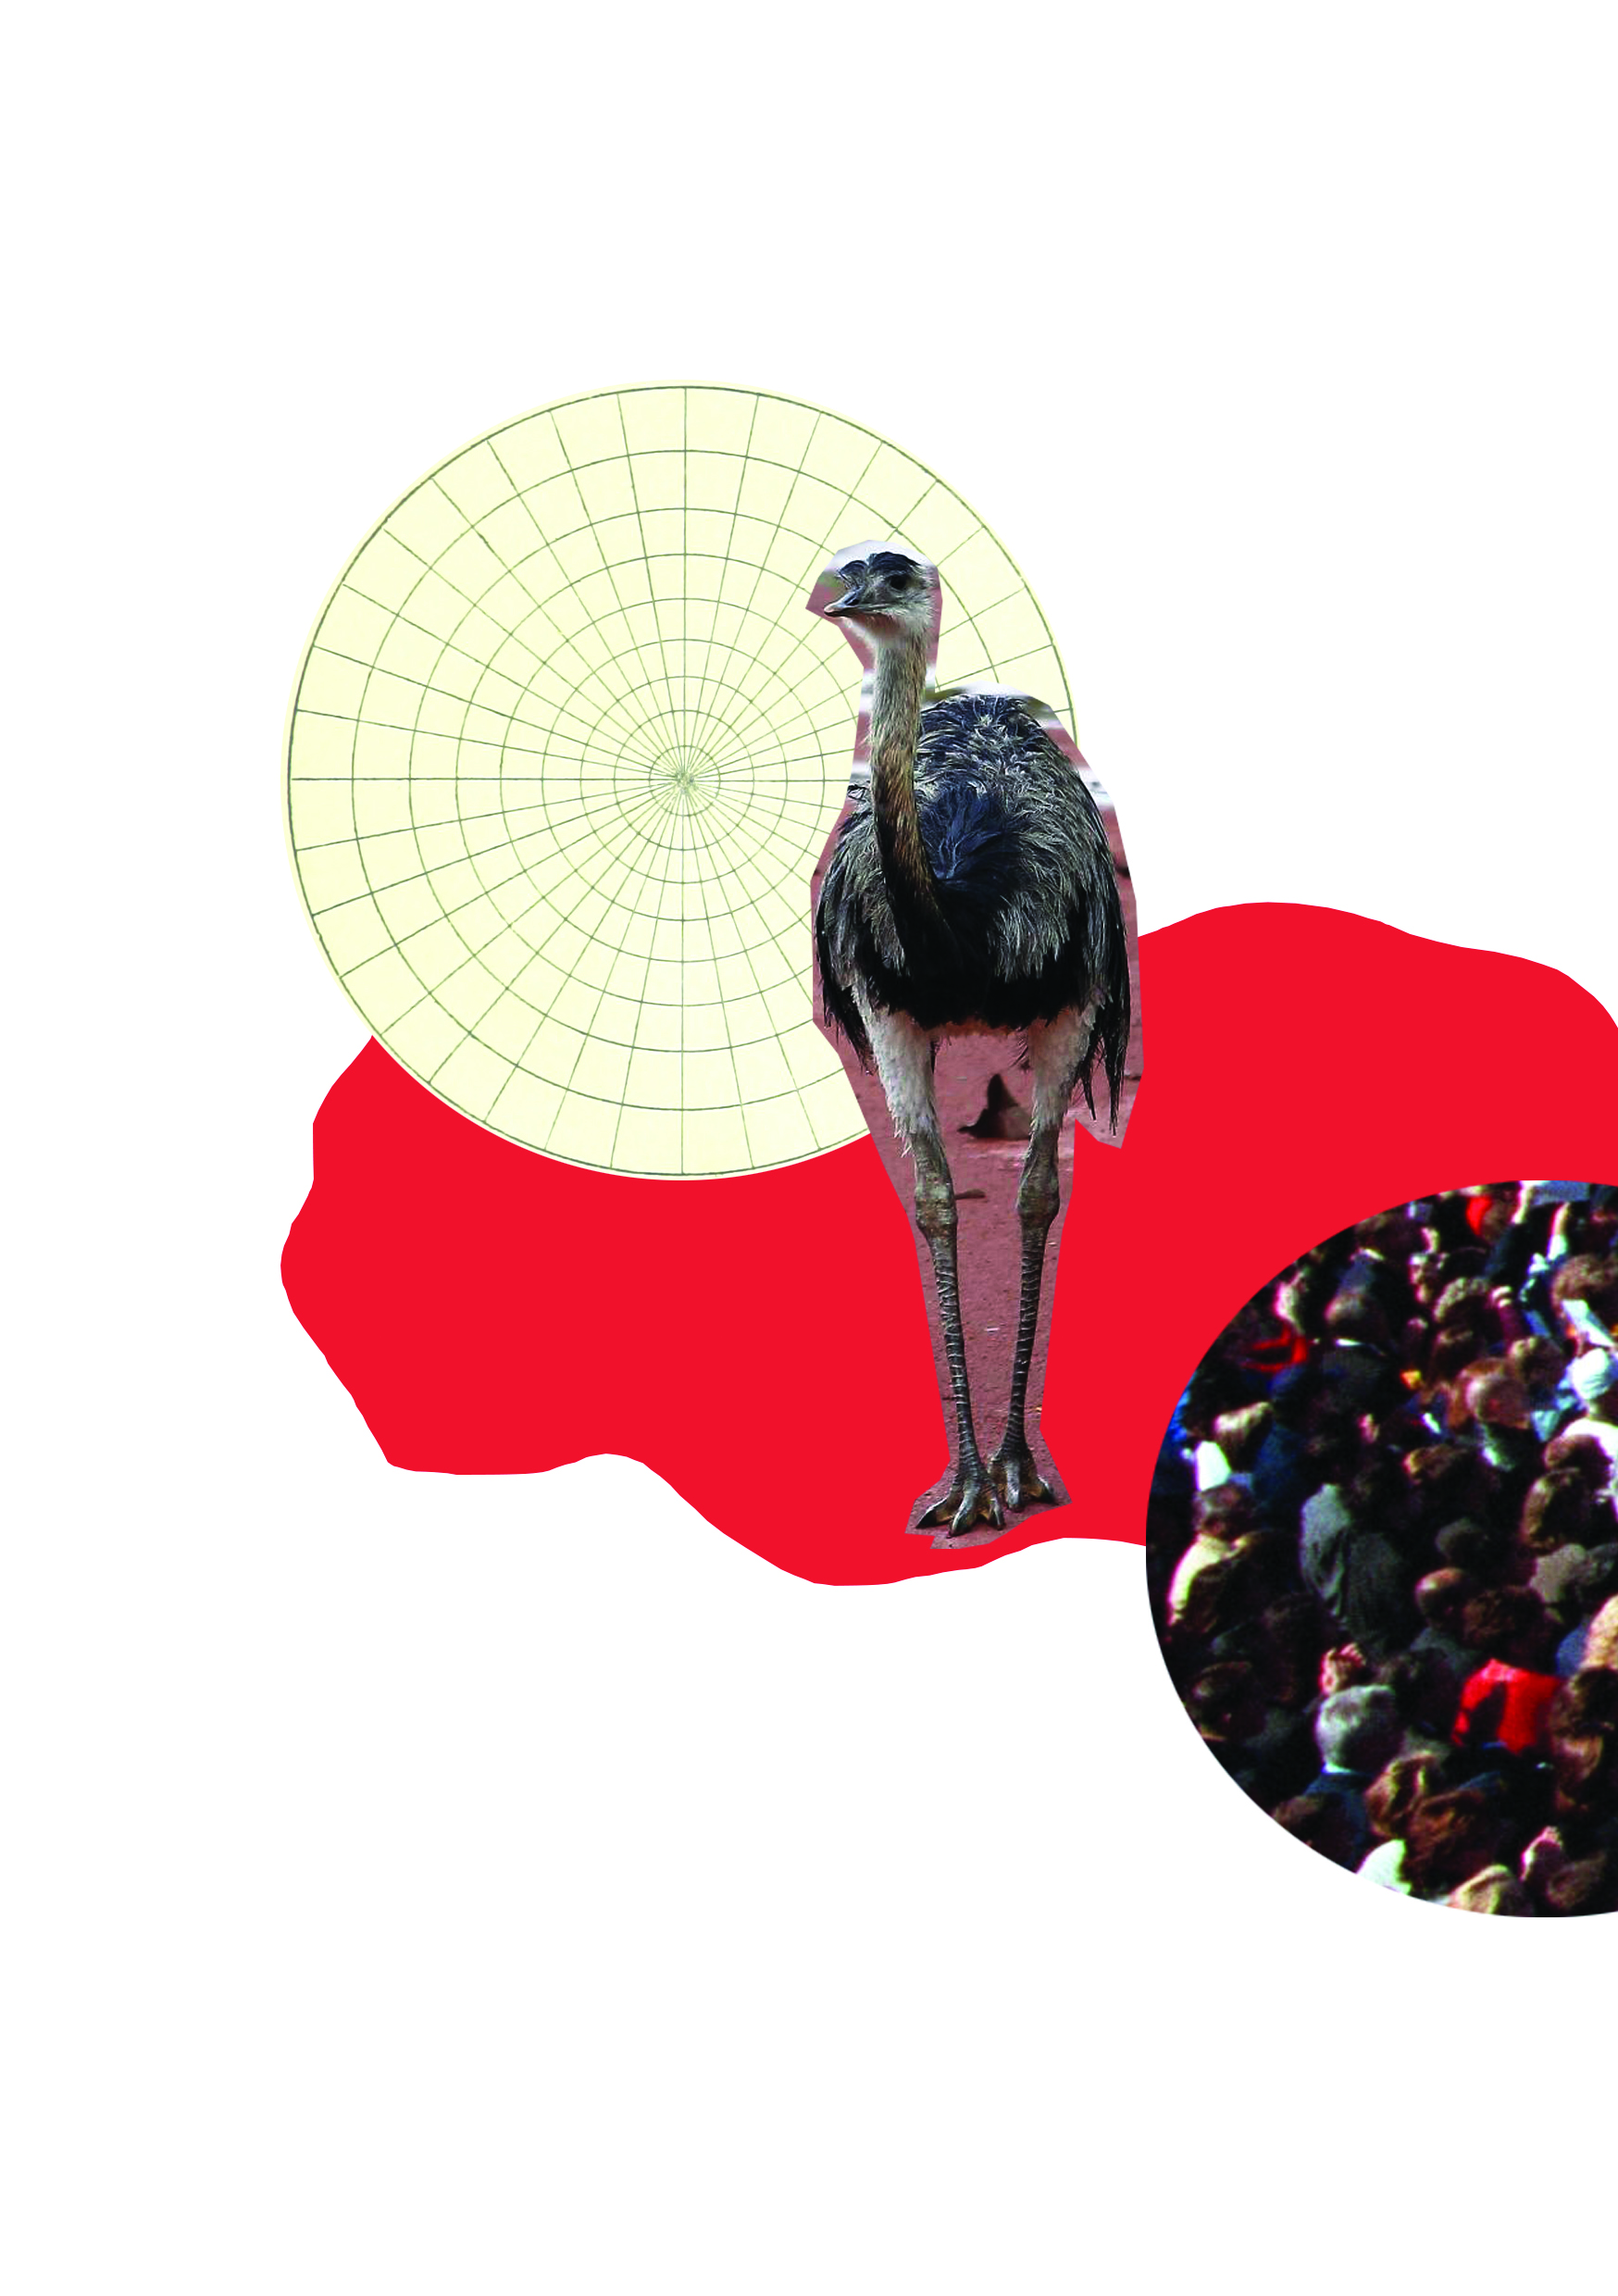
\includegraphics[width=140mm]{../ilustracoes/08_PEQUENINOS.jpg}
\end{figure}
\pagebreak

\chapterspecial{Os pequeninos}{}{Monteiro Lobato}

\noindent{}Ouvi certa vez uma conversa inesquecível. A esponja de doze anos não a
esmaeceu\footnote{esmaecer: desbotar, apagar.} em coisa nenhuma. Por que
motivo certas impressões se gravam de tal maneira e outras se apagam tão
profundamente?

Eu estava no cais, à espera do \emph{Arlanza}, que me ia devolver de
Londres um velho amigo já de longa ausência. O nevoeiro atrasara o
navio.

--- Só vai atracar às dez horas --- informou-me um sabe-tudo de boné.

Bem. Tinha eu de matar uma hora de espera dentro dum nevoeiro
absolutamente fora do comum, dos que negam aos olhos o consolo da
paisagem distante. A visão morria a dez passos; para além, todas as
formas desapareciam no algodoamento da névoa. Pensei nos
\emph{fogs}\footnote{\emph{fog}: nevoeiro denso.} londrinos que o meu
amigo devia trazer na alma e comecei a andar por ali à toa, entregue a
esse trabalho, tão frequente na vida, de ``matar o tempo''. Minha
técnica em tais circunstâncias se resume em recordar passagens da vida.
Recordar é reviver. Reviver os bons momentos tem as delícias do sonho.

Mas o movimento do cais interrompia amiúde o meu sonho, forçando-me a
cortar e a reatar de novo o fio das recordações. Tão cheio de nós foi
ele ficando que o abandonei. Uma das interrupções me pareceu mais
interessante que a evocação do passado, porque a vida exterior é mais
viva que a interior --- e a conversa dos três carregadores era
inegavelmente ``água-forte''.

Três portugueses bem típicos, já maduros; um deles de rosto
singularmente amarrotado pelos anos. Um incidente qualquer ali do cais
dera origem à conversa.

--- Pois esse caso, meu velho --- dizia um deles ---, me lembra a
história da ema que tive num cercado. Também ela foi vítima dum
animalzinho muitíssimo menor, e que seria esmagado, como esmagamos
moscas, se lhe ficasse ao alcance do bico --- mas não ficava\ldots{}

Esse começo assanhou a curiosidade dos companheiros.

--- Como foi? --- perguntaram.

--- Eu nesse tempo estava de cima, dono de terras, com casa minha, meus
animais de cocheira, família. Foi um ano antes daquela rodada que me
levou tudo\ldots{} Peste de mundo! Tão bem que eu ia indo e afundei, perdi
tudo, tive de rolar morro abaixo até bater com o lombo neste cais,
entregue ao mais baixo dos serviços, que é o de carregador\ldots{}

--- Mas como foi o caso da ema?

Os ouvintes não queriam filosofias; ansiavam por pitoresco\footnote{pitoresco:
  recreativo, original, envolvente.} --- e o homem por fim contou,
depois de sacar o cachimbo, enchê-lo, acendê-lo. Devia ser história das
que exigem pontuação a baforadas.

--- Eu morava em minhas terras, lá onde vocês sabem --- na Vacaria, zona
de campos e mais campos, aquela planura sem-fim. E há lá muita ema.
Conhecem? É a avestruz do Brasil, menor que a avestruz africana, mas
mesmo assim um avejão dos mais alentados. Que força tem! Domar uma ema
corresponde a domar um potro. Exige o mesmo muque. Mas são aves de boa
índole. Domesticam-se facilmente e eu andava querendo ter uma em meus
cercados.

--- São de utilidade? --- perguntou o utilitário da roda.

--- De nenhuma; apenas enfeitam a casa. Aparece um visitante. ``Viu
minha ema?'' --- e lá o levamos a examiná-la de perto, a assombrar-se do
tamanhão, a abrir a boca diante dos ovos. São assim como uma
laranja-baiana das graúdas.

--- E o gosto?

--- Nunca provei. Ovos para mim só os de galinha. Mas, como ia dizendo,
fiquei com ideia de apanhar uma ema nova para domesticá-la --- e um belo
dia eu mesmo o consegui graças à ajuda dum quiriquiri.

A história começava a interessar. Os companheiros do narrador ouviam-no
suspensos.

--- Como foi? Ande logo.

--- Foi num dia em que saí a cavalo para uma chegada à fazendinha do
João Coruja, que morava a uns seis quilômetros do meu rancho. Montei no
meu pampa e fui varando a macega. Aquilo lá não há caminho, só trilhas
de vai-um pelo capim rasteiro. Os olhos alcançam longe naquele mar de
verde sujo que some na distância. Fui andando. De repente vi a uns
trezentos metros longe qualquer coisa que se movia na macega.\footnote{macega:
  campina com capim alto e seco.} Parei. Firmei a vista. Era uma ema a
dar voltas num círculo estreito. ``Que diabo disto será aquilo?'',
perguntei comigo mesmo. Emas eu vira muitas, mas sempre a pastarem
sossegadas ou a fugirem no galope, nadando com as asas curtas. Assim a
dar voltas era novidade. Fiquei de rugas na testa. Que será? A gente da
roça conhece muito bem a natureza de tudo; se vê qualquer coisa na
``forma da lei'', não se espanta porque é o natural; mas se vê qualquer
coisa fora da lei, fica logo de orelha em pé --- porque não é o natural.
Que tinha aquela ema para dar tantas voltas em torno do mesmo ponto? Não
era da lei. A curiosidade me fez esquecer o negócio do João Coruja.
Torci a rédea ao pampa e lá me fui para a ema.

--- E ela fugiu no galope\ldots{}

--- O natural seria isso, mas não fugiu. Ora, não há ema que não fuja do
homem --- nem ema, nem animal nenhum. Nós somos o terror da bicharia
toda. Parei o pampa a cinco passos dela e nada, nada da ema fugir. Nem
me viu; continuou nas suas voltas, com ar aflito. Pus-me a observá-la,
intrigado. Seria seu ninho ali? Não era. Não havia sinal de ninho. A
pobre ave girava e regirava, fazendo movimentos de pescoço sempre na
mesma direção, para a esquerda, como se quisesse alcançar qualquer coisa
com o bico. A roda que fazia era de raio curto, aí duns três metros, e
pelo amassamento do capim calculei que já havia dado umas cem voltas.

--- Interessante! --- murmurou um dos companheiros.

--- Foi o que pensei comigo mesmo. Mais que interessante:
esquisitíssimo. Primeiro, não fugir de mim; segundo, continuar nas
voltas aflitas, sempre com aqueles movimentos de pescoço para a
esquerda. Que seria? Apeei e fui chegando. Olhei-a de bem perto. ``A
coisa é embaixo da asa'', vi logo. A pobre criatura tinha qualquer coisa
sob a asa, e aquelas voltas e aquele movimento de pescoço eram para
alcançar o sovaco. Aproximei-me mais. Segurei-a. A ema, arquejante, não
fez a menor resistência. Deixou-se agarrar. Ergui-lhe a asa e vi\ldots{}

Os ouvintes suspenderam o fôlego.

--- \ldots{} e vi uma coisa vermelha atracada ali, uma coisa que se assustou
e voou, e foi pousar num galho seco a vinte passos de distância. Sabem o
que era? Um quiriquiri\ldots{}

--- Que é isso?

--- Um gaviãozinho dos menores que existem, assim do tamanho dum sanhaço
--- um gaviãozinho-carijó.

--- Mas não disse que era vermelho?

--- Estava vermelho do sangue da ema. Agarrara-se-lhe ao sovaco, que é
um ponto despido de penas, e aferrara-se à carne com as unhas, enquanto
com o bico ia arrancando nacos de carne viva e devorando-os. Aquele
ponto do sovaco é o único sem defesa num corpo de ema, porque ela não o
alcança com o bico. É como esse ponto que temos nas costas e não podemos
coçar com as unhas. O quiriquiri conseguira localizar-se ali e estava a
seguro de bicadas.

``Examinei a ferida. Pobre ema! Uma ferida enorme, assim dum palmo de
diâmetro e onde o bico do quiriquiri fizera menos mal que suas garras,
pois, como tinha de manter-se aferrado, ia mudando as garras à proporção
que a carne dilacerada cedia. Nunca vi ferida mais arrepiante.''

--- Coitada!

--- As emas são duma estupidez famosa, mas o sofrimento abriu a
inteligência daquela. Fê-la compreender que eu era o seu salvador --- e
a mim entregou-se como quem se entrega a um deus. O alívio que minha
chegada lhe produziu, fazendo que o quiriquiri a largasse, iluminou-lhe
os miolos.

--- E o gaviãozinho?

--- Ah, o patife, muito vermelho do sangue da ema, lá ficou no galho
seco à espera de que eu me afastasse. Pretendia retomar ao banquete!
``Eu já te curo, malvado!'', exclamei, sacando o revólver. Um tiro.
Errei. O quiriquiri voou para longe.

--- E a ema?

--- Levei-a para casa, curei-a e tive-a lá por uns meses num cercado.
Por fim soltei-a. Não vai comigo isso de escravizar os pobres
animaizinhos que Deus fez para vida solta. Se no cercado estava livre
dos quiriquiris, era em compensação uma escrava saudosa das correrias
pelo campo. Se fosse consultada, certamente que preferiria os riscos da
liberdade à segurança da escravidão. Soltei-a. ``Vai, minha filha, segue
o teu destino. Se outro quiriquiri te apanhar, arruma-te lá com ele.''

--- Mas então é assim?

--- Um velho caboclo da zona informou-me que aquilo é frequente. Esses
minúsculos gaviõezinhos procuram as emas. Ficam traiçoeiramente a
rondá-las, à espera de que se descuidem e levantem a asa. Eles, então,
rápidos como setas, lançam-se; e se conseguem alcançar-lhes o sovaco,
ali enterram as garras e ficam como carrapatos. E as emas, apesar de
imensas comparadas com eles, acabam vencidas. Caem exaustas; morrem; e
os malvadinhos repastam-se no carname durante dias.

--- Mas como eles sabem? É o que mais admiro\ldots{}

--- Ah, meu caro, a natureza está inçada de coisas assim, que para nós
são mistérios. Com certeza houve um quiriquiri que por acaso fez isso
uma primeira vez, e como deu certo ensinou a lição aos outros. Estou
convencido de que os animais ensinam uns aos outros o que vão
aprendendo. Oh, vocês, criaturas da cidade, não imaginam que coisas
interessantes há na natureza da roça\ldots{}

O caso da ema foi comentado sob todos os ângulos --- e deu um broto. Fez
sair da memória do carregador de cara amarrotada uma história vagamente
similar, em que bichinhos muito pequenos destruíram a vida moral dum
homem.

--- Sim, destruíram a vida dum bicho imensamente maior, como sou eu em
comparação com as formigas. Fiquem vocês sabendo que a mim aconteceu
coisa ainda pior que o acontecido à ema. Fui vítima dum formigueiro\ldots{}

Todos arregalaram os olhos.

--- Só se já foste hortelão e as formigas te comeram a fazenda ---
sugeriu um.

--- Nada disso. Comeram-me mais que a fazenda, comeram-me a alma.
Destruíram-me moralmente --- mas foi sem querer. Pobrezinhas! Não as
culpo de nada.

--- Conta lá isso depressa!, Manuel. O \emph{Arlanza} não tarda.

E o velho contou.

--- Eu era o fiel da firma Toledo \& Cia., com obrigação de tomar conta
daquele grande armazém da rua Tal. Vocês sabem que tomar conta dum
depósito de mercadorias é coisa séria, porque o homem se torna o único
responsável por tudo quanto entra e sai. Ora, eu, português dos antigos,
desses de antes quebrar que torcer, fui escolhido para ``fiel'' porque
era fiel --- era e sou. Não valho nada, sou um pobre homem ao léu, mas
honradez está aqui. Meu orgulho sempre foi esse. Criei reputação desde
menino. ``O Manuel é dos bons; quebra mas não torce.'' Pois não é que as
formigas me quebraram?

--- Conta lá isso depressa\ldots{}

--- A coisa foi assim. Na qualidade de fiel do armazém, nada entrava nem
saía sem ser por minhas mãos. Eu fiscalizava tudo e com tal severidade
que Toledo \& Cia. juravam sobre mim como sobre a Bíblia. Certa vez
entrou lá uma partida de trinta e dois sacos de arroz, que contei,
conferi e fiz empilhar a um canto, junto a uma pilha de velhos caixões
que lá estavam encostados de muito tempo. Trinta e dois. Contei-os e
recontei-os e escrevi no livro de entradas trinta e dois, nem mais um,
nem menos um. E no dia seguinte, conforme velho hábito meu, ainda me fui
à pilha e recontei os sacos. Trinta e dois.

``--- Pois muito que bem. O tempo se passa. O arroz lá fica meses à
espera de negócio, até que um dia recebo do escritório ordem para
entregá-lo ao portador. Vou dirigir a entrega. Fico na porta do armazém
conferindo os sacos que por ali passavam à costas de dois carregadores
--- um, dois, vinte, trinta e um\ldots{} Faltava o último.

``---Anda com isso! --- berrei ao carregador que fora buscá-lo, mas o
bruto aparece-me lá dos fundos com as mãos vazias:

``---Não há mais nada.

``---Como não há mais nada? --- exclamei. --- São trinta e dois. Falta
um. Vá buscá-lo, vá ver.

``Ele foi e voltou na mesma:

``---Não há mais nada.

``---Impossível!

``E fui eu mesmo fazer a verificação e nada achei. Misteriosamente
desaparecera um saco de arroz da pilha\ldots{}

``--- Aquilo pôs-me tonto de cabeça. Esfreguei os olhos. Cocei-me.
Voltei ao livro de entradas; reli o assento; claro como o dia: trinta e
dois. Além disso eu lembrava-me muito bem daquela partida por causa dum
incidente agradável. Logo que terminei a contagem eu havia dito `trinta
e dois, última dezena do camelo!', e aproveitei o palpite na venda da
esquina. Mil réis na dezena trinta e dois: de tarde apareceu-me o
empregadinho com oitenta mil réis. Dera o camelo com trinta e dois.

``--- Vocês bem sabem que essas coisas a gente não esquece. Eram pois
trinta e duas sacas --- e como então só estavam lá trinta e uma? Pus-me a
parafusar. Furtar ninguém furtara, porque eu era o mais fiel dos fiéis,
não arredava pé da porta e dormia lá dentro. Janelas gradeadas de ferro.
Porta, uma só. Que ninguém furtara o saco de arroz era coisa que eu
juraria perante todos os tribunais do mundo, como o jurava para a minha
consciência. Mas a saca de arroz desaparecera\ldots{} e como era?

``--- Tive de comunicar ao escritório o desaparecimento --- e foi o
maior vexame da minha vida. Porque nós, operários, temos a nossa honra,
e a minha honra era aquela --- era ser o único responsável por tudo
quanto entrasse e saísse daquele depósito.

``Chamaram-me ao escritório.

``---Como explica a diferença, Manuel?

``Cocei a cabeça.

``---Meu senhor --- respondi ao patrão --- bem quisera eu explicá-la, mas
por mais que torça os miolos não consigo. Recebi os trinta e dois sacos
de arroz; contei-os e recontei-os, e tanto eram trinta e dois que nesse
dia deu essa dezena e `mamei' do vendeiro da esquina oitenta `paus'. O
arroz demorou lá meses. Agora recebo ordem para entregá-lo ao caminhão.
Vou presidir à retirada e só encontro trinta e um. Furtá-lo, ninguém o
furtou; isso juro, porque a entrada do armazém é uma só e eu sempre fui
cão de fila --- mas o fato é que o saco de arroz desapareceu. Não sei
explicar o mistério.

``As casas comerciais têm que seguir certas normas, e se eu fosse o
patrão faria o que ele fez. Já que era o Manuel o responsável único, se
não havia explicação para o mistério, pior para o Manuel.

``--- Manuel --- disse o patrão --- a nossa confiança em você sempre foi
completa, como você muito bem sabe, confiança de doze anos; mas o arroz
não podia ter-se evaporado como água ao fogo. E como desapareceu um saco
podem desaparecer mil. Quero que você mesmo nos diga o que devemos
fazer.

``Respondi como devia.

``--- O que há a fazer, meu senhor, é despedir o Manuel. Ninguém furtou
a saca de arroz, mas a saca de arroz confiada à guarda do Manuel
desapareceu. O que o patrão tem a fazer é fazer o que o Manuel faria se
estivesse em seu lugar: despedi-lo e contratar outro.

``O patrão disse:

``--- Muito lamento ter de agir assim, Manuel, mas tenho sócios que me
fiscalizam os atos, e serei criticado se não fizer como você mesmo me
aconselha.''

O velho carregador parou para avivar o cachimbo.

--- E foi assim, meus caros, que depois de doze anos de serviço no
armazém de Toledo \& Cia. fui para o olho da rua, suspeitado de ladrão
por todos os meus colegas. Se ninguém podia furtar aquele arroz e o
arroz desaparecera, qual o culpado? O Manuel, evidentemente.

``Fui para a rua, meus caros, já velhusco e sem carta de recomendação,
porque recusei a que a firma me quis dar por esmola. Em boa consciência,
que carta poderiam dar-me os senhores Toledo \& Cia.?

``Ah, o que sofri! Saber-me inocente e sentir-me suspeitado --- e sem
meios de defesa. Roubar é roubar, seja mil rés, sejam contos. Cesteiro
que faz um cesto faz um cento. E eu, que era um homem feliz porque
compensava a minha pobreza com a fama de honestidade sem par, rolei para
a classe dos duvidosos. E o pior era o rato que me roía os miolos. Os
outros podiam satisfazer-se atribuindo a mim o furto, mas eu, que sabia
da minha inocência, não arrancava aquele rato da cabeça. Quem tiraria de
lá o saco de arroz? Esse pensamento ficou-me lá dentro como um berne dos
cabeludos.

``Dois anos se passaram, em que envelheci dez. Um dia recebo recado da
firma, `que aparecesse no escritório'. Fui.

``--- Manuel --- disse-me o mesmo chefe que me despedira --- o
misterioso desaparecimento do saco de arroz está decifrado e você
reabilitado da maneira mais completa. Ladrões tiraram de lá o arroz sem
que você visse\ldots{}

``--- Não pode ser, meu senhor! Tenho orgulho do meu trabalho de guarda.
Sei que ninguém entrou lá durante aqueles meses. Sei.

``O chefe sorriu.

``--- Pois saiba que inúmeros ladrõezinhos entraram e saíram com o
arroz.

``Fiquei tonto. Abri a boca.

``--- Sim, as formigas\ldots{}

``--- As formigas? Não estou entendendo nada, patrão\ldots{}

``Ele contou então tudo. A partida dos trinta e dois sacos fora
arrumada, como já disse, junto a uma pilha de velhos caixões vazios. E o
último saco ficava pouco acima do nível do último caixão --- disso eu me
lembrava perfeitamente. Fora esse o saco desaparecido. Pois bem. Um belo
dia o escritório dá ordem ao novo fiel para remover de lá os caixões. O
fiel executa-a --- mas ao fazê-lo nota uma coisa: grãos de arroz
derramados no chão, em redor dum olheiro de formigas saúvas. Foram as
saúvas as roubadoras da saca de arroz número trinta e dois!''

--- Como?

--- Subiram pelos interstícios\footnote{interstício: fenda, greta,
  pequeno espaço vazio.} da caixotaria e furaram o saco último, o qual
ficava um pouco acima do nível do último caixão. E foram retirando os
grãos um a um. Com o progressivo esvaziar-se, o saco perdeu o equilíbrio
e escorregou da pilha para cima do último caixão --- e nessa posição as
formigas completaram o esvaziamento\ldots{}

--- E\ldots{}

--- Os senhores Toledo \& Cia. pediram-me desculpas e ofereceram-me de
novo o lugar, com paga melhorada a título de indenização. Sabem o que
respondi?

``Meus senhores, é tarde. Já não me sinto o mesmo. O desastre matou-me
por dentro. Um rato roubou-me todo o arroz que havia dentro de mim.
Deixou-me o que sou: carregador do porto, saco vazio. Já não tenho
interesse em nada. Continuarei portanto carregador. É serviço de menos
responsabilidade --- além de que este mundo é uma pinoia. Pois um mundo
onde uns bichinhos inocentes dão cabo da alma dum homem, então isso é lá
mundo? Obrigado, meus senhores!'', e saí.

Nesse momento o \emph{Arlanza} apitou. O grupo dissolveu-se e também eu
fui colocar-me a postos. O amigo de Londres causou-me má impressão.
Magro, corcovado.

--- Que te aconteceu, Marinho?

--- Estou com os pulmões afetados.

Hum!, sempre a mesma coisa --- o pequenininho a derrear o grande.
Quiriquiri, saúva, bacilo de Koch\ldots{}\footnote{bacilo de Koch:
  bactéria transmissora da tuberculose.}

\blankpage

\pagebreak
\thispagestyle{empty}
\begin{figure}
\vspace*{-.5cm}
\hspace*{-2.3cm}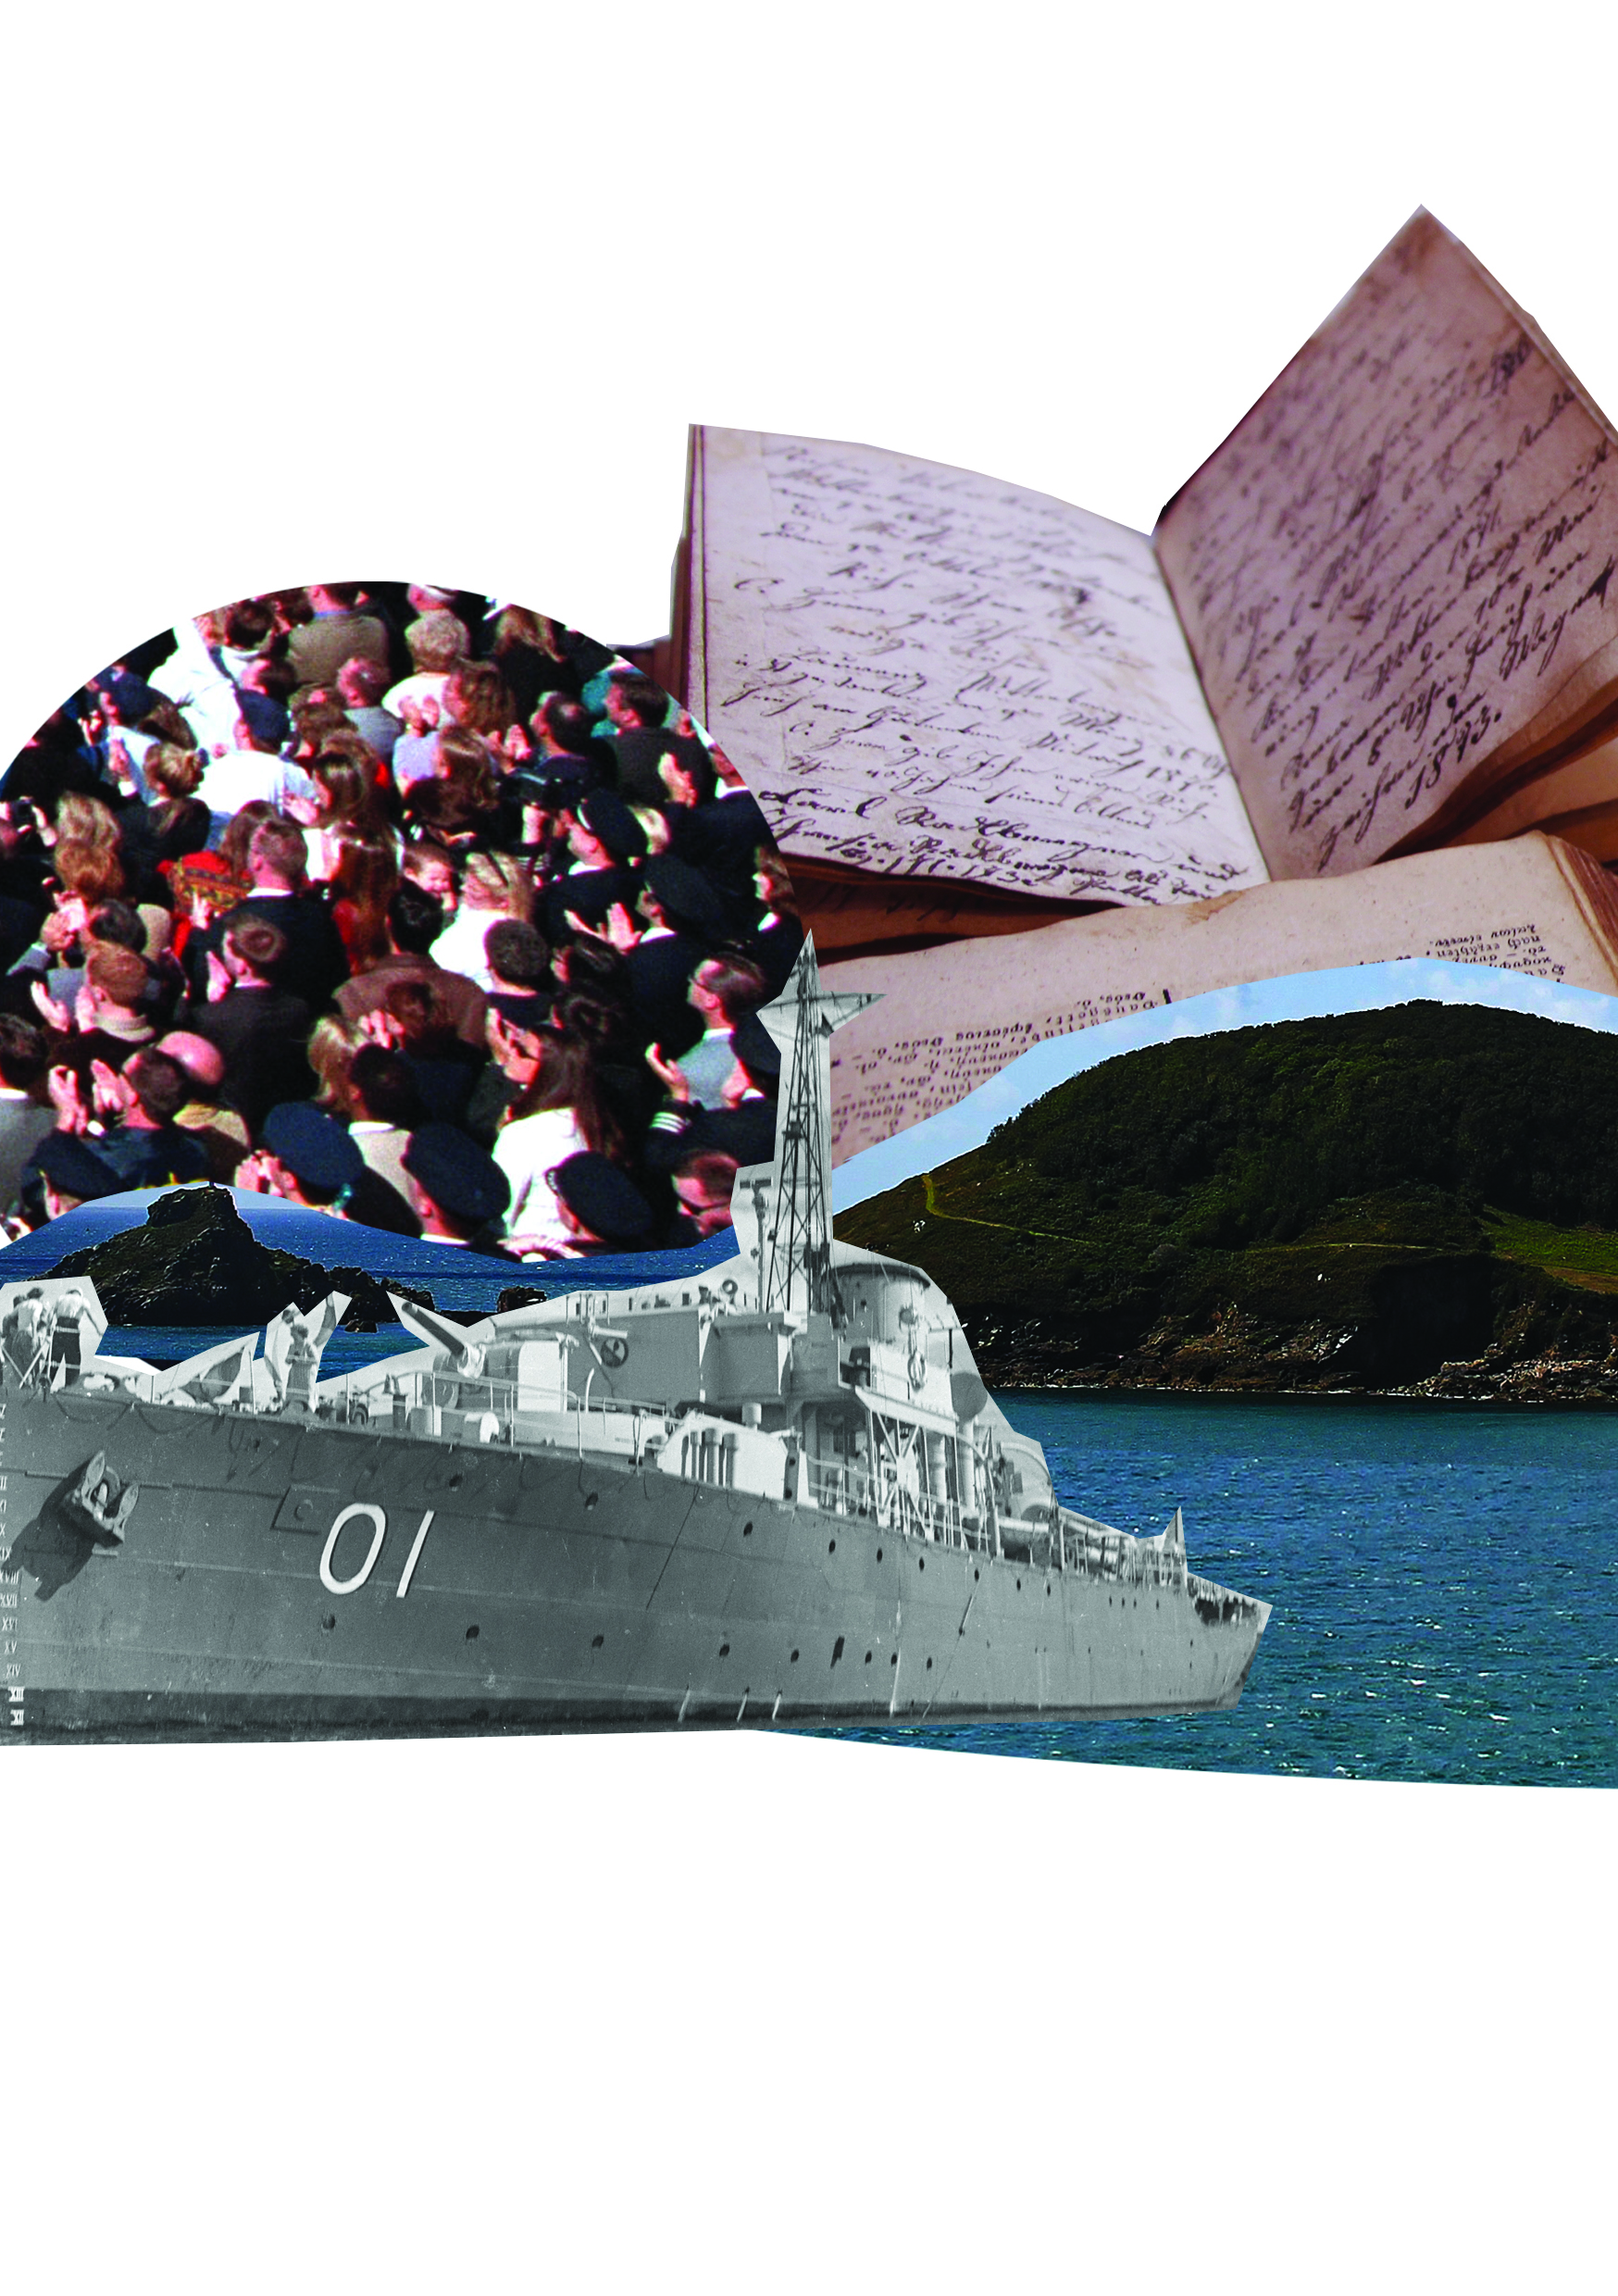
\includegraphics[width=140mm]{../ilustracoes/09_JAVANES.jpg}
\end{figure}
\pagebreak

\chapterspecial{O homem que sabia javanês}{}{Lima Barreto}

\noindent{}Em uma confeitaria, certa vez, ao meu amigo Castro, contava eu as
partidas que havia pregado às convicções e às respeitabilidades, para
poder viver.

Houve mesmo, uma dada ocasião, quando estive em Manaus, em que fui
obrigado a esconder a minha qualidade de bacharel, para mais confiança
obter dos clientes, que afluíam ao meu escritório de feiticeiro e
adivinho. Contava eu isso.

O meu amigo ouvia-me calado, embevecido, gostando daquele meu Gil Blas
vivido, até que, em uma pausa da conversa, ao esgotarmos os copos,
observou a esmo:

--- Tens levado uma vida bem engraçada, Castelo!

--- Só assim se pode viver\ldots{} Isto de uma ocupação única: sair de
casa a certas horas, voltar a outras, aborrece, não achas? Não sei como
me tenho aguentado lá, no consulado!

--- Cansa-se; mas, não é disso que me admiro. O que me admira, é que
tenhas corrido tantas aventuras aqui, neste Brasil imbecil e
burocrático.

--- Qual! Aqui mesmo, meu caro Castro, se podem arranjar belas páginas
de vida. Imagina tu que eu já fui professor de javanês!

--- Quando? Aqui, depois que voltaste do consulado?

--- Não; antes. E, por sinal, fui nomeado cônsul por isso.

--- Conta lá como foi. Bebes mais cerveja?

--- Bebo.

Mandamos buscar mais outra garrafa, enchemos os copos, e continuei:

--- Eu tinha chegado havia pouco ao Rio e estava literalmente na
miséria. Vivia fugido de casa de pensão em casa de pensão, sem saber
onde e como ganhar dinheiro, quando li no \emph{Jornal do Commercio} o
anúncio seguinte:

``Precisa-se de um professor de língua javanesa. Cartas, etc.''

Ora, disse cá comigo, está aí uma colocação que não terá muitos
concorrentes; se eu capiscasse quatro palavras, ia apresentar-me. Saí do
café e andei pelas ruas, sempre a imaginar-me professor de javanês,
ganhando dinheiro, andando de bonde e sem encontros desagradáveis com os
\emph{cadáveres}. Insensivelmente dirigi-me à Biblioteca Nacional. Não
sabia bem que livro iria pedir; mas, entrei, entreguei o chapéu ao
porteiro, recebi a senha e subi. Na escada, acudiu-me pedir a
\emph{Grande Encyclopédie}, letra \emph{J}, a fim de consultar o artigo
relativo a Java e à língua javanesa. Dito e feito. Fiquei sabendo, ao
fim de alguns minutos, que Java era uma grande ilha do arquipélago de
Sonda, colônia holandesa, e o javanês, língua aglutinante do grupo
maleo-polinésico, possuía uma literatura digna de nota e escrita em
caracteres derivados do velho alfabeto hindu.

A \emph{Encyclopédie} dava-me indicação de trabalhos sobre a tal língua
malaia e não tive dúvidas em consultar um deles. Copiei o alfabeto, a
sua pronunciação figurada e saí. Andei pelas ruas, perambulando e
mastigando letras.

Na minha cabeça dançavam hieróglifos;\footnote{hieróglifo: unidade
  ideográfica fundamental do sistema de escrita do antigo Egito, que
  aparece nas inscrições sobre os monumentos.} de quando em quando
consultava as minhas notas; entrava nos jardins e escrevia estes
calungas na areia para guardá-los bem na memória e habituar a mão a
escrevê-los.

À noite, quando pude entrar em casa sem ser visto, para evitar
indiscretas perguntas do encarregado, ainda continuei no quarto a
engolir o meu \emph{a b c} malaio,\footnote{malaio: língua
  malaio-polinésia falada na Malásia, na Tailândia, em Cingapura,
  Brunei, Indonésia e áreas circunvizinhas, que apresenta certa
  fragmentação dialetal.} e, com tanto afinco levei o propósito que, de
manhã, o sabia perfeitamente.

Convenci-me que aquela era a língua mais fácil do mundo e saí; mas não
tão cedo que não me encontrasse com o encarregado dos aluguéis dos
cômodos:

--- Senhor Castelo, quando salda a sua conta?

Respondi-lhe então eu, com a mais encantadora esperança:

--- Breve\ldots{} Espere um pouco\ldots{} Tenha paciência\ldots{} Vou
ser nomeado professor de javanês, e\ldots{}

Por aí o homem interrompeu-me:

--- Que diabo vem a ser isso, senhor Castelo?

Gostei da diversão e ataquei o patriotismo do homem:

--- É uma língua que se fala lá pelas bandas do Timor. Sabe onde é?

Oh! alma ingênua! O homem esqueceu-se da minha dívida e disse-me com
aquele falar forte dos portugueses:

--- Eu cá por mim, não sei bem; mas ouvi dizer que são umas terras que
temos lá para os lados de Macau. E o senhor sabe isso, senhor Castelo?

Animado com esta saída feliz que me deu o javanês, voltei a procurar o
anúncio. Lá estava ele. Resolvi animosamente propor-me ao professorado
do idioma oceânico. Redigi a resposta, passei pelo \emph{Jornal} e lá
deixei a carta. Em seguida, voltei à biblioteca e continuei os meus
estudos de javanês. Não fiz grandes progressos nesse dia, não sei se por
julgar o alfabeto javanês o único saber necessário a um professor de
língua malaia ou se por ter me empenhado mais na bibliografia e história
literária do idioma que ia ensinar.

Ao cabo de dois dias, recebia eu uma carta para ir falar ao doutor
Manuel Feliciano Soares Albernaz, barão de Jacuecanga, à rua Conde de
Bonfim, não me recordo bem que número. É preciso não te esqueceres que
entrementes continuei estudando o meu malaio, isto é, o tal javanês.
Além do alfabeto, fiquei sabendo o nome de alguns autores, também
perguntar e responder --- \emph{Como está o senhor?} --- e duas ou três
regras de gramática, lastrado todo esse saber com vinte palavras do
léxico.\footnote{léxico: vocabulário.}

Não imaginas as grandes dificuldades com que lutei, para arranjar os
quatrocentos réis da viagem! É mais fácil --- podes ficar certo ---
aprender o javanês\ldots{} Fui a pé. Cheguei suadíssimo; e, com maternal
carinho, as anosas mangueiras, que se perfilavam em alameda diante da
casa do titular, me receberam, me acolheram e me reconfortaram. Em toda
a minha vida, foi o único momento em que cheguei a sentir a simpatia da
natureza\ldots{}

Era uma casa enorme que parecia estar deserta; estava mal tratada, mas
não sei por que me veio pensar que nesse mau tratamento havia mais
desleixo e cansaço de viver que mesmo pobreza. Devia haver anos que não
era pintada. As paredes descascavam e os beirais do telhado, daquelas
telhas vidradas de outros tempos, estavam desguarnecidos aqui e ali,
como dentaduras decadentes ou mal cuidadas.

Olhei um pouco o jardim e vi a pujança vingativa com que a tiririca e o
carrapicho tinham expulsado os tinhorões e as begônias. Os crótons
continuavam, porém, a viver com a sua folhagem de cores mortiças. Bati.
Custaram-me a abrir. Veio, por fim, um antigo preto africano, cujas
barbas e cabelo de algodão davam à sua fisionomia uma aguda impressão de
velhice, doçura e sofrimento.

Na sala, havia uma galeria de retratos: arrogantes senhores de barba em
colar se perfilavam enquadrados em imensas molduras douradas, e doces
perfis de senhoras, em bandós, com grandes leques, pareciam querer subir
aos ares, enfunadas pelos redondos vestidos à balão; mas, daquelas
velhas coisas, sobre as quais a poeira punha mais antiguidade e
respeito, a que gostei mais de ver foi um belo jarrão de porcelana da
China ou da Índia, como se diz. Aquela pureza da louça, a sua
fragilidade, a ingenuidade do desenho e aquele seu fosco brilho de luar,
diziam-me a mim que aquele objeto tinha sido feito por mãos de criança,
a sonhar, para encanto dos olhos fatigados dos velhos
desiludidos\ldots{}

Esperei um instante o dono da casa. Tardou um pouco. Um tanto
trôpego,\footnote{trôpego: que anda com dificuldade.} com o lenço de
alcobaça na mão, tomando veneravelmente o simonte\footnote{simonte:
  fumo, rapé, pó resultante de folhas de tabaco torradas e moídas, por
  vezes misturadas a outros componentes aromáticos, usado para inalação,
  e que provoca espirros.} de antanho,\footnote{antanho: tempo passado.}
foi cheio de respeito que o vi chegar. Tive vontade de ir-me embora.
Mesmo se não fosse ele o discípulo, era sempre um crime mistificar
aquele ancião, cuja velhice trazia à tona do meu pensamento alguma coisa
de augusto, de sagrado. Hesitei, mas fiquei.

--- Eu sou --- avancei --- o professor de javanês, que o senhor disse
precisar.

--- Sente-se --- respondeu-me o velho. --- O senhor é daqui, do Rio?

--- Não, sou de Canavieiras.

--- Como? --- fez ele. --- Fale um pouco alto, que sou surdo.

--- Sou de Canavieiras, Bahia --- insisti eu.

--- Onde fez os seus estudos?

--- Em São Salvador.

--- E onde aprendeu o javanês? --- indagou ele, com aquela teimosia
peculiar aos velhos.

Não contava com essa pergunta, mas imediatamente arquitetei uma mentira.
Contei-lhe que meu pai era javanês. Tripulante de um navio mercante,
viera ter à Bahia, estabelecera-se nas proximidades de Canavieiras como
pescador, casara, prosperara e fora com ele que aprendi javanês.

--- E ele acreditou? E o físico? --- perguntou meu amigo, que até então
me ouvira calado.

--- Não sou --- objetei --- lá muito diferente de um javanês. Estes meus
cabelos corridos, duros e grossos e a minha pele \emph{basané} podem
dar-me muito bem o aspecto de um mestiço de malaio\ldots{} Tu sabes bem
que, entre nós, há de tudo: índios, malaios, taitianos, malgaches,
guanches, até godos. É uma comparsaria de raças e tipos de fazer inveja
ao mundo inteiro.

--- Bem --- fez o meu amigo ---, continua.

--- O velho --- emendei eu --- ouviu-me atentamente, considerou
demoradamente o meu físico, pareceu que me julgava de fato filho de
malaio e perguntou-me com doçura:

--- Então está disposto a ensinar-me javanês?

A resposta saiu-me sem querer: --- Pois não.

--- O senhor há de ficar admirado --- aduziu o Barão de Jacuecanga ---
que eu, nesta idade, ainda queira aprender qualquer coisa, mas\ldots{}

--- Não tenho que admirar. Têm-se visto exemplos e exemplos muito
fecundos\ldots{}

--- O que eu quero, meu caro senhor\ldots{}

--- Castelo --- adiantei eu.

--- O que eu quero, meu caro senhor Castelo, é cumprir um juramento de
família. Não sei se o senhor sabe que eu sou neto do conselheiro
Albernaz, aquele que acompanhou Pedro I, quando abdicou. Voltando de
Londres, trouxe para aqui um livro em língua esquisita, a que tinha
grande estimação. Fora um hindu ou siamês que lho dera, em Londres, em
agradecimento a não sei que serviço prestado por meu avô. Ao morrer meu
avô, chamou meu pai e lhe disse: ``Filho, tenho este livro aqui, escrito
em javanês. Disse-me quem mo deu que ele evita desgraças e traz
felicidades para quem o tem. Eu não sei nada ao certo. Em todo o caso,
guarda-o; mas, se queres que o fado que me deitou o sábio oriental se
cumpra, faze com que teu filho o entenda, para que sempre a nossa raça
seja feliz''.

--- Meu pai --- continuou o velho barão --- não acreditou muito na
história; contudo, guardou o livro. Às portas da morte, ele mo deu e
disse-me o que prometera ao pai. Em começo, pouco caso fiz da história
do livro. Deitei-o a um canto e fabriquei minha vida. Cheguei até a
esquecer-me dele; mas, de uns tempos a esta parte, tenho passado por
tanto desgosto, tantas desgraças têm caído sobre a minha velhice que me
lembrei do talismã da família. Tenho que o ler, que o compreender, se
não quero que os meus últimos dias anunciem o desastre da minha
posteridade; e, para entendê-lo, é claro, que preciso entender o
javanês. Eis aí.

Calou-se e notei que os olhos do velho se tinham orvalhado.\footnote{orvalhar:
  molhar.} Enxugou discretamente os olhos e perguntou-me se queria ver o
tal livro. Respondi-lhe que sim. Chamou o criado, deu-lhe as instruções
e explicou-me que perdera todos os filhos, sobrinhos, só lhe restando
uma filha casada, cuja prole, porém, estava reduzida a um filho, débil
de corpo e de saúde frágil e oscilante.

Veio o livro. Era um velho calhamaço,\footnote{calhamaço: livro ou
  caderno volumoso.} um in-quarto\footnote{in-quarto: folha de impressão
  dobrada duas vezes, de que resulta um caderno com quatro folhas ou
  oito páginas.} antigo, encadernado em couro, impresso em grandes
letras, em um papel amarelado e grosso. Faltava a folha do rosto e por
isso não se podia ler a data da impressão. Tinha ainda umas páginas de
prefácio, escritas em inglês, onde li que se tratava das histórias do
príncipe Kulanga, escritor javanês de muito mérito.

Logo informei disso o velho barão que, não percebendo que eu tinha
chegado aí pelo inglês, ficou tendo em alta consideração o meu saber
malaio. Estive ainda folheando o cartapácio, à laia de quem sabe
magistralmente aquela espécie de vasconço, até que afinal contratamos as
condições de preço e de hora, comprometendo-me a fazer com que ele lesse
o tal alfarrábio antes de um ano.

Dentro em pouco, dava a minha primeira lição, mas o velho não foi tão
diligente quanto eu. Não conseguia aprender a distinguir e a escrever
nem sequer quatro letras. Enfim, com metade do alfabeto levamos um mês e
o senhor barão de Jacuecanga não ficou lá muito senhor da matéria:
aprendia e desaprendia.

A filha e o genro (penso que até aí nada sabiam da história do livro)
vieram a ter notícias do estudo do velho; não se incomodaram. Acharam
graça e julgaram a coisa boa para distraí-lo.

Mas com o que tu vais ficar assombrado, meu caro Castro, é com a
admiração que o genro ficou tendo pelo professor de javanês. Que coisa
única! Ele não se cansava de repetir: ``É um assombro! Tão moço! Se eu
soubesse isso, ah! onde estava!''.

O marido de dona Maria da Glória (assim se chamava a filha do barão),
era desembargador, homem relacionado e poderoso; mas não se pejava em
mostrar diante de todo o mundo a sua admiração pelo meu javanês. Por
outro lado, o barão estava contentíssimo. Ao fim de dois meses,
desistira da aprendizagem e pedira-me que lhe traduzisse, um dia sim
outro não, um trecho do livro encantado. Bastava entendê-lo, disse-me
ele; nada se opunha que outrem o traduzisse e ele ouvisse. Assim evitava
a fadiga do estudo e cumpria o encargo.

Sabes bem que até hoje nada sei de javanês, mas compus umas histórias
bem tolas e impingi-as ao velhote como sendo do crônicon. Como ele ouvia
aquelas bobagens!\ldots{}

Ficava extático,\footnote{extático: encantado, enlevado, maravilhado.}
como se estivesse a ouvir palavras de um anjo. E eu crescia aos seus
olhos!

Fez-me morar em sua casa, enchia-me de presentes, aumentava-me o
ordenado. Passava, enfim, uma vida regalada.

Contribuiu muito para isso o fato de vir ele a receber uma herança de um
seu parente esquecido que vivia em Portugal. O bom velho atribuiu a
coisa ao meu javanês; e eu estive quase a crê-lo também.

Fui perdendo os remorsos; mas, em todo o caso, sempre tive medo que me
aparecesse pela frente alguém que soubesse o tal patuá malaio. E esse
meu temor foi grande, quando o doce barão me mandou com uma carta ao
visconde de Caruru, para que me fizesse entrar na diplomacia. Fiz-lhe
todas as objeções: a minha fealdade, a falta de elegância, o meu aspecto
tagalo. ``--- Qual! --- retrucava ele. --- Vá, menino; você sabe
javanês!'' Fui. Mandou-me o visconde para a Secretaria dos Estrangeiros
com diversas recomendações. Foi um sucesso.

O diretor chamou os chefes de seção: ``Vejam só, um homem que sabe
javanês --- que portento!''.\footnote{portento: maravilha.}

Os chefes de seção levaram-me aos oficiais e amanuenses e houve um
destes que me olhou mais com ódio do que com inveja ou admiração. E
todos diziam: ``Então sabe javanês? É difícil? Não há quem o saiba
aqui!''.

O tal amanuense, que me olhou com ódio, acudiu então: ``É verdade, mas
eu sei canaque. O senhor sabe?''. Disse-lhe que não e fui à presença do
ministro.

A alta autoridade levantou-se, pôs as mãos às cadeiras, concertou o
pincenê no nariz e perguntou: ``Então, sabe javanês?''. Respondi-lhe que
sim; e, à sua pergunta onde o tinha aprendido, contei-lhe a história do
tal pai javanês. ``Bem, disse-me o ministro, o senhor não deve ir para a
diplomacia; o seu físico não se presta\ldots{} O bom seria um consulado
na Ásia ou Oceania. Por ora, não há vaga, mas vou fazer uma reforma e o
senhor entrará. De hoje em diante, porém, fica adido ao meu ministério e
quero que, para o ano, parta para Bale, onde vai representar o Brasil no
Congresso de Linguística. Estude, leia o Hovelacque, o Max Müller, e
outros!''

Imagina tu que eu até aí nada sabia de javanês, mas estava empregado e
iria representar o Brasil em um congresso de sábios.

O velho barão veio a morrer, passou o livro ao genro para que o fizesse
chegar ao neto, quando tivesse a idade conveniente e fez-me uma deixa no
testamento.

Pus-me com afã no estudo das línguas maleo-polinésicas; mas não havia
meio!

Bem jantado, bem vestido, bem dormido, não tinha energia necessária para
fazer entrar na cachola aquelas coisas esquisitas. Comprei livros,
assinei revistas: \emph{Revue Anthropologique et Linguistique},
\emph{Proceedings of the English-Oceanic Association}, \emph{Archivo
Glottologico Italiano}, o diabo, mas nada! E a minha fama crescia. Na
rua, os informados apontavam-me, dizendo aos outros: ``Lá vai o sujeito
que sabe javanês''. Nas livrarias, os gramáticos consultavam-me sobre a
colocação dos pronomes no tal jargão das ilhas de Sonda. Recebia cartas
dos eruditos do interior, os jornais citavam o meu saber e recusei
aceitar uma turma de alunos sequiosos de entenderem o tal javanês. A
convite da redação, escrevi no \emph{Jornal do Commercio} um artigo de
quatro colunas sobre a literatura javanesa antiga e moderna\ldots{}

--- Como, se tu nada sabias? --- interrompeu-me o atento Castro.

--- Muito simplesmente: primeiramente, descrevi a ilha de Java, com o
auxílio de dicionários e umas poucas de geografias, e depois citei a
mais não poder.

--- E nunca duvidaram? --- perguntou-me ainda o meu amigo.

--- Nunca. Isto é, uma vez quase fico perdido. A polícia prendeu um
sujeito, um marujo, um tipo bronzeado que só falava uma língua
esquisita. Chamaram diversos intérpretes, ninguém o entendia. Fui também
chamado, com todos os respeitos que a minha sabedoria merecia,
naturalmente. Demorei-me em ir, mas fui afinal. O homem já estava solto,
graças à intervenção do cônsul holandês, a quem ele se fez compreender
com meia dúzia de palavras holandesas. E o tal marujo era javanês ---
uf!

Chegou, enfim, a época do congresso, e lá fui para a Europa. Que
delícia! Assisti à inauguração e às sessões preparatórias.
Inscreveram-me na seção do tupi-guarani e eu abalei para Paris. Antes,
porém, fiz publicar no \emph{Mensageiro de Bale} o meu retrato, notas
biográficas e bibliográficas. Quando voltei, o presidente pediu-me
desculpas por me ter dado aquela seção; não conhecia os meus trabalhos e
julgara que, por ser eu americano brasileiro, me estava naturalmente
indicada a seção do tupi-guarani. Aceitei as explicações e até hoje
ainda não pude escrever as minhas obras sobre o javanês, para lhe
mandar, conforme prometi.

Acabado o congresso, fiz publicar extratos do artigo do \emph{Mensageiro
de Bale}, em Berlim, em Turim e Paris, onde os leitores de minhas obras
me ofereceram um banquete, presidido pelo senador Gorot. Custou-me toda
essa brincadeira, inclusive o banquete que me foi oferecido, cerca de
dez mil francos, quase toda a herança do crédulo e bom barão de
Jacuecanga.

Não perdi meu tempo nem meu dinheiro. Passei a ser uma glória nacional
e, ao saltar no cais Pharoux, recebi uma ovação de todas as classes
sociais e o presidente da República, dias depois, convidava-me para
almoçar em sua companhia.

Dentro de seis meses fui despachado cônsul em Havana, onde estive seis
anos e para onde voltarei, a fim de aperfeiçoar os meus estudos das
línguas da Malaia, Melanésia e Polinésia.

--- É fantástico --- observou Castro, agarrando o copo de cerveja.

--- Olha: se não fosse estar contente, sabes que ia ser?

--- Quê?

--- Bacteriologista eminente.\footnote{eminente: importante.} Vamos?

--- Vamos.

\part{Nas relações amorosas}

\pagebreak
\thispagestyle{empty}
\begin{figure}
\vspace*{-.5cm}
\hspace*{-2.3cm}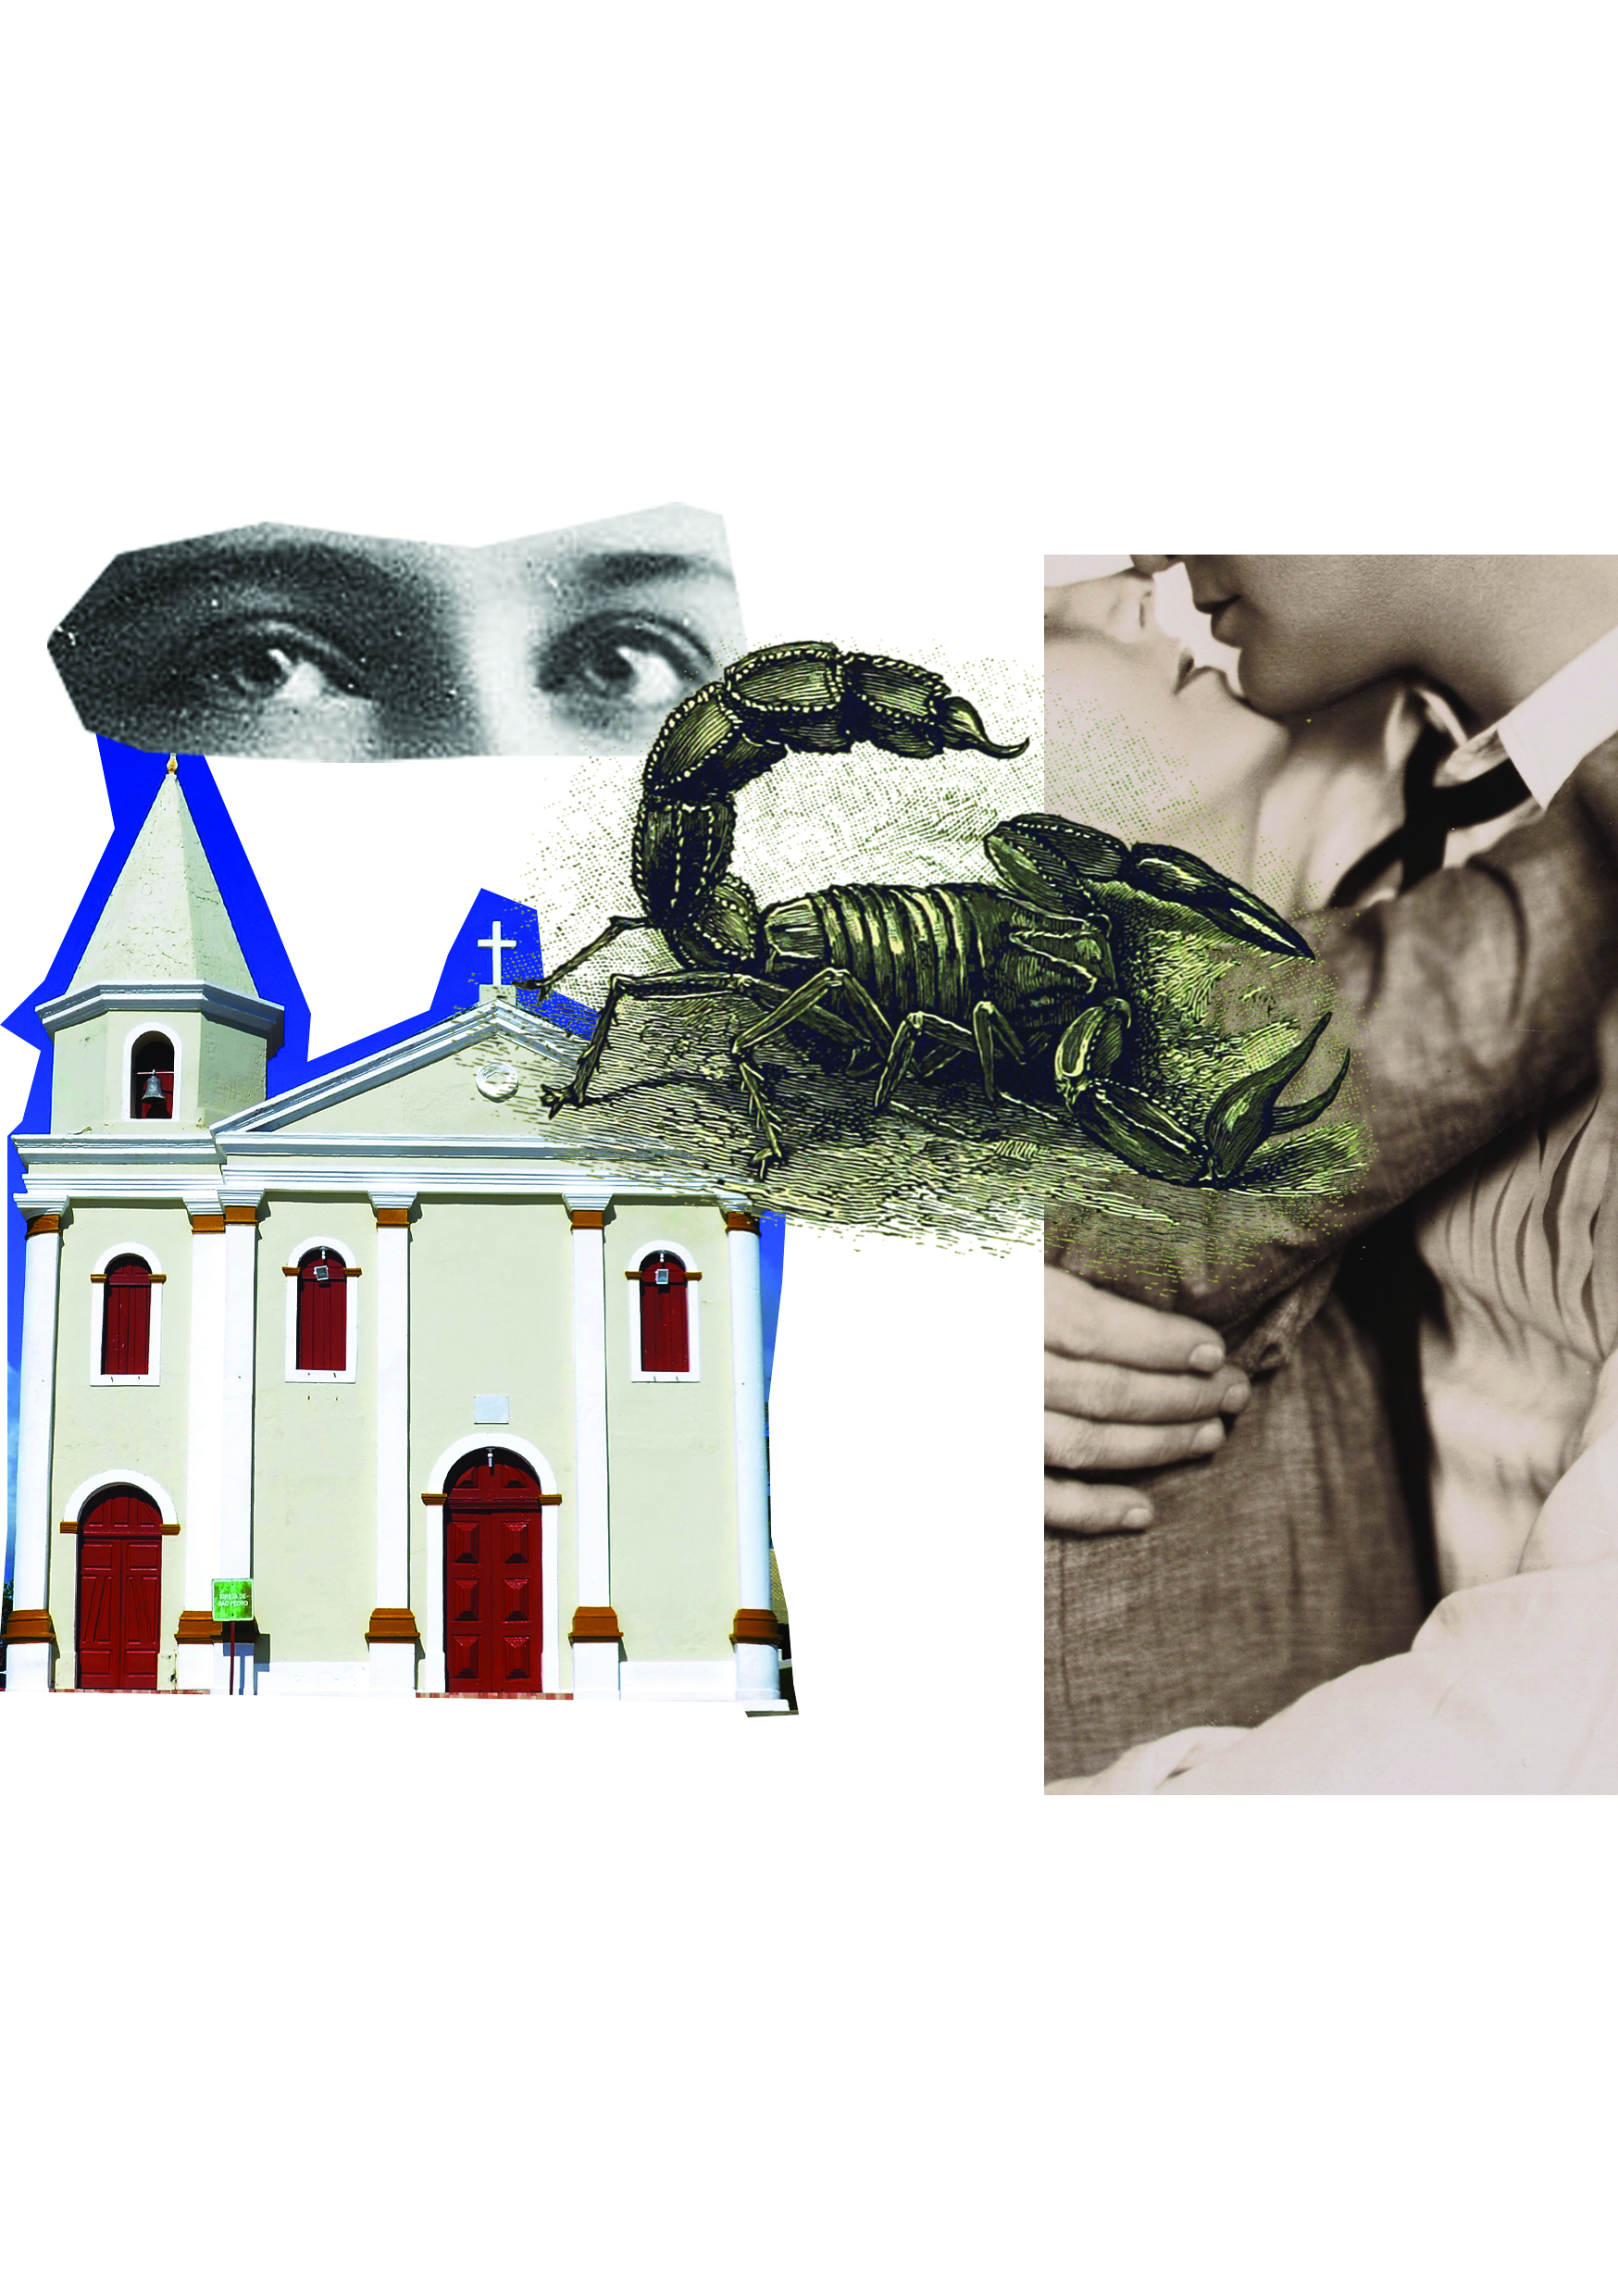
\includegraphics[width=140mm]{../ilustracoes/10_PRIMAS.jpg}
\end{figure}
\pagebreak

\chapterspecial{Primas de Sapucaia!}{}{Machado de Assis}

\noindent{}Há umas ocasiões oportunas e fugitivas, em que o acaso nos inflige duas
ou três primas de Sapucaia; outras vezes, ao contrário, as primas de
Sapucaia são antes um benefício do que um infortúnio.

Era à porta de uma igreja. Eu esperava que as minhas primas Claudina e
Rosa tomassem água benta, para conduzi-las à nossa casa, onde estavam
hospedadas. Tinham vindo de Sapucaia, pelo Carnaval, e demoraram-se dois
meses na Corte. Era eu que as acompanhava a toda a parte, missas,
teatros, rua do Ouvidor, porque minha mãe, com o seu reumático, mal
podia mover-se dentro de casa, e elas não sabiam andar sós. Sapucaia era
a nossa pátria comum. Embora todos os parentes estivessem dispersos, ali
nasceu o tronco da família. Meu tio José Ribeiro, pai destas primas, foi
o único, de cinco irmãos, que lá ficou lavrando a terra e figurando na
política do lugar. Eu vim cedo para a Corte, donde segui a estudar e
bacharelar-me em São Paulo. Voltei uma só vez a Sapucaia, para pleitear
uma eleição, que perdi.

Rigorosamente, todas estas notícias são desnecessárias para a
compreensão da minha aventura; mas é um modo de ir dizendo alguma coisa,
antes de entrar em matéria, para a qual não acho porta grande nem
pequena; o melhor é afrouxar a rédea à pena, e ela que vá andando, até
achar entrada. Há de haver alguma; tudo depende das circunstâncias,
regra que tanto serve para o estilo como para a vida; palavra puxa
palavra, uma ideia traz outra, e assim se faz um livro, um governo, ou
uma revolução; alguns dizem mesmo que assim é que a natureza compôs as
suas espécies.

Portanto, água benta e porta de igreja. Era a igreja de São José. A
missa acabara; Claudina e Rosa fizeram uma cruz na testa, com o dedo
polegar, molhado na água benta e descalçado unicamente para esse gesto.
Depois ajustaram os manteletes, enquanto eu, ao portal, ia vendo as
damas que saíam. De repente, estremeço, inclino-me para fora, chego
mesmo a dar dois passos na direção da rua.

--- Que foi, primo?

--- Nada, nada.

Era uma senhora, que passara rentezinha com a igreja, vagarosa,
cabisbaixa, apoiando-se no chapelinho de sol; ia pela rua da
Misericórdia acima. Para explicar a minha comoção, é preciso dizer que
era a segunda vez que a via. A primeira foi no Prado Fluminense, dois
meses antes, com um homem que, pelos modos, era seu marido, mas tanto
podia ser marido como pai. Estava então um pouco de espavento, vestida
de escarlate, com grandes enfeites vistosos, e umas argolas demasiado
grossas nas orelhas; mas os olhos e a boca resgatavam o resto. Namoramos
às bandeiras despregadas. Se disser que saí dali apaixonado, não meto a
minha alma no inferno, porque é a verdade pura. Saí tonto, mas saí
também desapontado, perdi-a de vista na multidão. Nunca mais pude dar
com ela, nem ninguém me soube dizer quem fosse.

Calcule-se o meu enfado, vendo que a fortuna vinha trazê-la outra vez ao
meu caminho, e que umas primas fortuitas não me deixavam lançar-lhe as
mãos. Não será difícil calculá-lo, porque estas primas de Sapucaia tomam
todas as formas, e o leitor, se não as teve de um modo, teve-as de
outro. Umas vezes copiam o ar confidencial de um cavalheiro informado da
última crise do ministério, de todas as causas aparentes ou secretas,
dissensões novas ou antigas, interesses agravados, conspiração, crise.
Outras vezes, enfronham-se na figura daquele eterno cidadão que afirma
de um modo ponderoso e abotoado, que não há leis sem costumes,
\emph{nisi lege sine moribus}.\footnote{\emph{nisi lege sine moribus}:
  frase latina baseada em verso de Horácio, ``Sem os costumes, as leis
  são inúteis''.} Outras, afivelam a máscara de um Dangeau de esquina,
que nos conta miudamente as fitas e rendas que esta, aquela, aqueloutra
dama levara ao baile ou ao teatro. E durante esse tempo, a Ocasião
passa, vagarosa, cabisbaixa, apoiando-se no chapelinho de sol: passa,
dobra a esquina, e adeus\ldots{} O ministério esfacelava-se; malinas e
bruxelas; \emph{nisi lege sine moribus}\ldots{}

Estive a pique de dizer às primas que se fossem embora; morávamos na rua
do Carmo, não era longe; mas abri mão da ideia. Já na rua pensei também
em deixá-las na igreja, à minha espera, e ir ver se agarrava a Ocasião
pela calva. Creio mesmo que cheguei a parar um momento, mas rejeitei
igualmente esse alvitre e fui andando.

Fui andando com elas para o lado oposto ao da minha incógnita. Olhei
para trás repetidas vezes, até perdê-la numa das curvas da rua, com os
olhos no chão, como quem reflete, devaneia ou espera uma hora marcada.
Não minto dizendo que esta última ideia trouxe-me a emoção do ciúme. Sou
exclusivo e pessoal; daria um triste amante de mulheres casadas. Não
importa que entre mim e aquela dama existisse apenas uma contemplação
fugitiva de algumas horas; desde que a minha personalidade ia para ela,
a partilha tornava-se-me insuportável. Sou também imaginoso; engenhei
logo uma aventura e um aventureiro, dei-me ao prazer mórbido de
afligir-me sem motivo nem necessidade. As primas iam adiante, e
falavam-me de quando em quando; eu respondia mal, se respondia alguma
cousa. Cordialmente, execrava-as.

Ao chegar à porta de casa, consultei o relógio, como se tivesse alguma
cousa que fazer; depois disse às primas que subissem e fossem almoçando.
Corri à rua da Misericórdia. Fui primeiro até à Escola de Medicina;
depois voltei e vim até à Câmara dos Deputados, então mais devagar,
esperando vê-la ao chegar a cada curva da rua; mas nem sombra. Era
insensato, não era? Todavia, ainda subi outra vez a rua, porque adverti
que, a pé e devagar, mal teria tempo de ir em meio da praia de Santa
Luzia, se acaso não parara antes; e aí fui, rua acima e praia fora, até
ao convento da Ajuda. Não encontrei nada, coisa nenhuma. Nem por isso
perdi as esperanças; arrepiei caminho e vim, a passo lento ou apressado,
conforme se me afigurava que era possível apanhá-la adiante, ou dar
tempo a que saísse de alguma parte. Desde que a minha imaginação
reproduzia a dama, todo eu sentia um abalo, como se realmente tivesse de
vê-la daí a alguns minutos. Compreendi a emoção dos doidos.

Entretanto, nada. Desci a rua sem achar o menor vestígio da minha
incógnita. Felizes os cães, que pelo faro dão com os amigos! Quem sabe
se não estaria ali bem perto, no interior de alguma casa, talvez a
própria casa dela? Lembrou-me indagar; mas de quem, e como? Um padeiro,
encostado ao portal, espiava-me; algumas mulheres faziam a mesma coisa
enfiando os olhos pelos postigos. Naturalmente desconfiavam do
transeunte, do andar vagaroso ou apressado, do olhar inquisidor, do
gesto inquieto. Deixei-me ir até à Câmara dos Deputados, e parei uns
cinco minutos, sem saber que fizesse. Era perto de meio-dia. Esperei
mais dez minutos, depois mais cinco, parado, com a esperança de vê-la;
afinal, desesperei e fui almoçar.

Não almocei em casa. Não queria ver os demônios das primas, que me
impediram de seguir a dama incógnita. Fui a um hotel. Escolhi uma mesa
no fim da sala, e sentei-me de costas para as outras; não queria ser
visto nem conversado. Comecei a comer o que me deram. Pedi alguns
jornais, mas confesso que não li nada seguidamente, e apenas entendi
três quartas partes do que ia lendo. No meio de uma notícia ou de um
artigo, escorregava-me o espírito e caía na rua da Misericórdia, à porta
da igreja, vendo passar a incógnita, vagarosa, cabisbaixa, apoiando-se
no chapelinho de sol.

A última vez que me aconteceu essa separação da outra e da besta, estava
já no café, e tinha diante de mim um discurso parlamentar. Achei-me
ainda uma vez à porta da igreja; imaginei então que as primas não
estavam comigo, e que eu seguia atrás da bela dama. Assim é que se
consolam os preteridos da loteria; assim é que se fartam as ambições
malogradas.

Não me peçam minúcias nem preliminares do encontro. Os sonhos desdenham
as linhas finas e o acabado das paisagens; contentam-se de quatro ou
cinco brochadas grossas, mas representativas. Minha imaginação galgou as
dificuldades da primeira fala, e foi direita à rua do Lavradio ou dos
Inválidos, à própria casa de Adriana. Chama-se Adriana. Não viera à rua
da Misericórdia por motivo de amores, mas a ver alguém, uma parenta ou
uma comadre, ou uma costureira. Conheceu-me, e teve igual comoção.
Escrevi-lhe; respondeu-me. Nossas pessoas foram uma para a outra por
cima de uma multidão de regras morais e de perigos. Adriana é casada; o
marido conta cinquenta e dois anos, ela, trinta imperfeitos. Não amou
nunca, não amou mesmo o marido, com quem casou por obedecer à família.
Eu ensinei-lhe ao mesmo tempo o amor e a traição; é o que ela me diz
nesta casinha que aluguei fora da cidade, de propósito para nós.

Ouço-a embriagado. Não me enganei; é a mulher ardente e amorosa, qual me
diziam os seus olhos, olhos de touro, como os de Juno,\footnote{Juno:
  conforme a mitologia clássica, Juno, ou Hera, é a mulher de Júpiter,
  ou Zeus.} grandes e redondos. Vive de mim e para mim. Escrevemo-nos
todos os dias; e, apesar disso, quando nos encontramos na casinha, é
como se mediara um século. Creio até que o coração dela ensinou-me
alguma coisa, embora noviço, ou por isso mesmo. Nesta matéria
desaprende-se com o uso e o ignorante é que é douto. Adriana não
dissimula a alegria nem as lágrimas; escreve o que pensa, conta o que
sente; mostra-me que não somos dois, mas um, tão somente um ente
universal, para quem Deus criou o sol e as flores, o papel e a tinta, o
correio e as carruagens fechadas.

Enquanto ideava isto, creio que acabei de beber o café; lembra-me que o
criado veio à mesa e retirou a xícara e o açucareiro. Não sei se lhe
pedi fogo, provavelmente viu-me com o charuto na mão e trouxe-me
fósforos.

Não juro, mas penso que acendi o charuto, porque daí a um instante,
através de um véu de fumaça, vi a cabeça meiga e enérgica da minha bela
Adriana, encostada a um sofá. Eu estou de joelhos, ouvindo-lhe a
narração da última rusga do marido. Que ele já desconfia; ela sai muitas
vezes, distrai-se, absorve-se, aparece-lhe triste ou alegre, sem motivo,
e o marido começa a ameaçá-la. Ameaçá-la de quê? Digo-lhe que, antes de
qualquer excesso, era melhor deixá-lo, para viver comigo, publicamente,
um para o outro. Adriana escuta-me pensativa, cheia de Eva, namorada do
demônio, que lhe sussurra de fora o que o coração lhe diz de dentro. Os
dedos afagam-me os cabelos.

--- Pois sim! Pois sim!

Veio no dia seguinte, consigo mesma, sem marido, sem sociedade, sem
escrúpulos, tão somente consigo, e fomos dali viver juntos. Nem
ostentação, nem resguardo. Supusemo-nos estrangeiros, e realmente não
éramos outra cousa; falávamos uma língua que nunca ninguém antes falara
nem ouvira. Os outros amores eram, desde séculos, verdadeiras
contrafações; nós dávamos a edição autêntica. Pela primeira vez,
imprimia-se o manuscrito divino, um grosso volume que nós dividíamos em
tantos capítulos e parágrafos quantas eram as horas do dia ou os dias da
semana. O estilo era tecido de sol e música; a linguagem compunha-se da
fina flor dos outros vocabulários. Tudo o que neles existia, meigo ou
vibrante, foi extraído pelo autor para formar esse livro único --- livro
sem índice, porque era infinito --- sem margens, para que o fastio não
viesse escrever nelas as suas notas, --- sem fita, porque já não
tínhamos precisão de interromper a leitura e marcar a página.

Uma voz chamou-me à realidade. Era um amigo que acordara tarde, e vinha
almoçar. Nem o sonho me deixava esta outra prima de Sapucaia! Cinco
minutos depois despedi-me e saí; eram duas horas passadas.

Vexa-me dizer que ainda fui à rua da Misericórdia, mas é preciso narrar
tudo: fui e não achei nada. Voltei nos dias seguintes sem outro lucro,
além do tempo perdido. Resignei-me a abrir mão da aventura, ou esperar a
solução do acaso. As primas achavam-me aborrecido ou doente; não lhes
disse que não. Daí a oito dias foram-se embora, sem me deixar saudades;
despedi-me delas como de uma febre maligna.

A imagem da minha incógnita\footnote{incógnita: mistério, enigma.} não
me deixou durante muitas semanas. Na rua, enganei-me várias vezes.
Descobria ao longe uma figura, que era tal qual a outra; picava os
calcanhares, até apanhá-la e desenganar-me. Comecei a achar-me ridículo;
mas lá vinha uma hora ou um minuto, uma sombra ao longe, e a preocupação
revivia. Afinal vieram outros cuidados, e não pensei mais nisso.

No princípio do ano seguinte, fui a Petrópolis; fiz a viagem com um
antigo companheiro de estudos, Oliveira, que foi promotor em Minas
Gerais, mas abandonara ultimamente a carreira por ter recebido uma
herança. Estava alegre como nos tempos da academia; mas de quando em
quando calava-se, olhando para fora da barca ou da caleça, com a atonia
de quem regala a alma de uma recordação, de uma esperança ou de um
desejo. No alto da serra perguntei-lhe para que hotel ia; respondeu que
ia para uma casa particular, mas não me disse aonde, e até desconversou.
Cuidei que me visitaria no dia seguinte; mas nem me visitou, nem o vi em
parte alguma. Outro colega nosso ouvira dizer que ele tinha uma casa
para os lados da Renânia.

Nenhuma destas circunstâncias voltaria à memória, se não fosse a notícia
que me deram dias depois. Oliveira tirara uma mulher ao marido, e fora
refugiar-se com ela em Petrópolis. Deram-me o nome do marido e o dela. O
dela era Adriana. Confesso que, embora o nome da outra fosse pura
invenção minha, estremeci ao ouvi-lo; não seria a mesma mulher? Vi logo
depois que era pedir muito ao acaso. Já faz bastante esse pobre oficial
das coisas humanas, concertando alguns fios dispersos; exigir que os
reate a todos, e com os mesmos títulos, é saltar da realidade na novela.
Assim falou o meu bom senso, e nunca disse tão gravemente uma tolice,
pois as duas mulheres eram nada menos que a mesmíssima.

Vi-a três semanas depois, indo visitar o Oliveira, que viera doente da
Corte. Subimos juntos na véspera; no meio da serra, começou ele a
sentir-se incomodado; no alto estava febril. Acompanhei-o no carro até a
casa, e não entrei, porque ele dispensou-me o incômodo. Mas no dia
seguinte fui vê-lo, um pouco por amizade, outro pouco por avidez de
conhecer a incógnita. Vi-a; era ela, era a minha, era a única Adriana.

Oliveira sarou depressa, e, apesar do meu zelo em visitá-lo, não me
ofereceu a casa; limitou-se a vir ver-me no hotel. Respeitei-lhe os
motivos; mas eles mesmos é que faziam reviver a antiga preocupação.
Considerei que, além das razões de decoro, havia da parte dele um
sentimento de ciúme, filho de um sentimento de amor, e que um e outro
podiam ser a prova de um complexo de qualidades finas e grandes naquela
mulher. Isto bastava a transtornar-me; mas a ideia de que a paixão dela
não seria menor que a dele, o quadro desse casal que fazia uma só alma e
pessoa, excitou em mim todos os nervos da inveja. Baldei esforços para
ver se metia o pé na casa; cheguei a falar-lhe do boato que corria; ele
sorria e tratava de outra coisa.

Acabou a estação de Petrópolis, e ele ficou. Creio que desceu em julho
ou agosto. No fim do ano encontramo-nos casualmente; achei-o um pouco
taciturno e preocupado. Vi-o ainda outras vezes, e não me pareceu
diferente, a não ser que, além de taciturno, trazia na fisionomia uma
longa prega de desgosto. Imaginei que eram efeitos da aventura, e, como
não estou aqui para empulhar ninguém, acrescento que tive uma sensação
de prazer. Durou pouco; era o demônio que trago em mim, e costuma fazer
desses esgares de saltimbanco. Mas castiguei-o depressa, e pus no lugar
dele o anjo, que também uso, e que se compadeceu do pobre rapaz,
qualquer que fosse o motivo da tristeza.

Um vizinho dele, amigo nosso, contou-me alguma coisa, que me confirmou a
suspeita de desgostos domésticos; mas foi ele mesmo quem me disse tudo,
um dia, perguntando-lhe eu, estouvadamente, o que é que tinha que o
mudara tanto.

--- Que hei de ter? Imagina tu que comprei um bilhete de loteria, e nem
tive, ao menos, o gosto de não tirar nada; tirei um escorpião.

E, como eu franzisse a testa interrogativamente:

--- Ah! Se soubesses metade só das coisas que me têm acontecido! Tens
tempo? Vamos aqui ao Passeio Público.

Entramos no jardim, e metemo-nos por uma das alamedas. Contou-me tudo.
Gastou duas horas em desfiar um rosário infinito de misérias. Vi através
da narração duas índoles incompatíveis, unidas pelo amor ou pelo pecado,
fartas uma da outra, mas condenadas à convivência e ao ódio. Ele nem
podia deixá-la nem suportá-la. Nenhuma estima, nenhum respeito, alegria
rara e impura; uma vida gorada.

--- Gorada --- repetia ele, gesticulando afirmativamente com a cabeça.
--- Não tem que ver; a minha vida gorou. Hás de lembrar-te dos nossos
planos da academia, quando nos propúnhamos, tu a ministro do Império,
eu, da Justiça. Podes guardar as duas pastas; não serei nada, nada. O
ovo, que devia dar uma águia, não chega a dar um frango. Gorou
completamente. Há ano e meio que ando nisso, e não acho saída nenhuma;
perdi a energia\ldots{}

Seis meses depois, encontrei-o aflito e desvairado. Adriana deixara-o
para ir estudar geometria com um estudante da antiga Escola Central. ---
Tanto melhor, disse-lhe eu. Oliveira olhou para o chão envergonhado;
despediu-se, e correu em procura dela. Achou-a daí a algumas semanas,
disseram as últimas um ao outro, e no fim reconciliaram-se. Comecei
então a visitá-los, com a ideia de os separar um do outro. Ela estava
ainda bonita e fascinante; as maneiras eram finas e meigas, mas
evidentemente de empréstimo, acompanhadas de umas atitudes e gestos,
cujo intuito latente era atrair-me e arrastar-me.

Tive medo e retraí-me. Não se mortificou; deitou fora a capa de renda,
restituiu-se ao natural. Vi então que era ferrenha, manhosa, injusta,
muita vez grosseira; em alguns lances notei-lhe uma nota de
perversidade. Oliveira, nos primeiros tempos, para fazer-me crer que
mentira ou exagerara, suportava tudo rindo; era a vergonha da própria
fraqueza. Mas não pôde guardar a máscara; ela arrancou-lha um dia, sem
piedade, denunciando as humilhações em que ele caía, quando eu não
estava presente. Tive nojo da mulher e pena do pobre-diabo. Convidei-o
abertamente a deixá-la, ele hesitou, mas prometeu que sim.

--- Realmente, não posso mais\ldots{}

Combinamos tudo; mas no momento da separação, não pôde. Ela embebeu-lhe
novamente os seus grandes olhos de touro e de basilisco,\footnote{basilisco:
  lagarto ou serpente fabulosa, cujo olhar teria o poder de matar.} e
desta vez, --- ó minhas queridas primas de Sapucaia! --- desta vez para
só deixá-lo exausto e morto.

\pagebreak
\thispagestyle{empty}
\begin{figure}
\vspace*{-.5cm}
\hspace*{-2.3cm}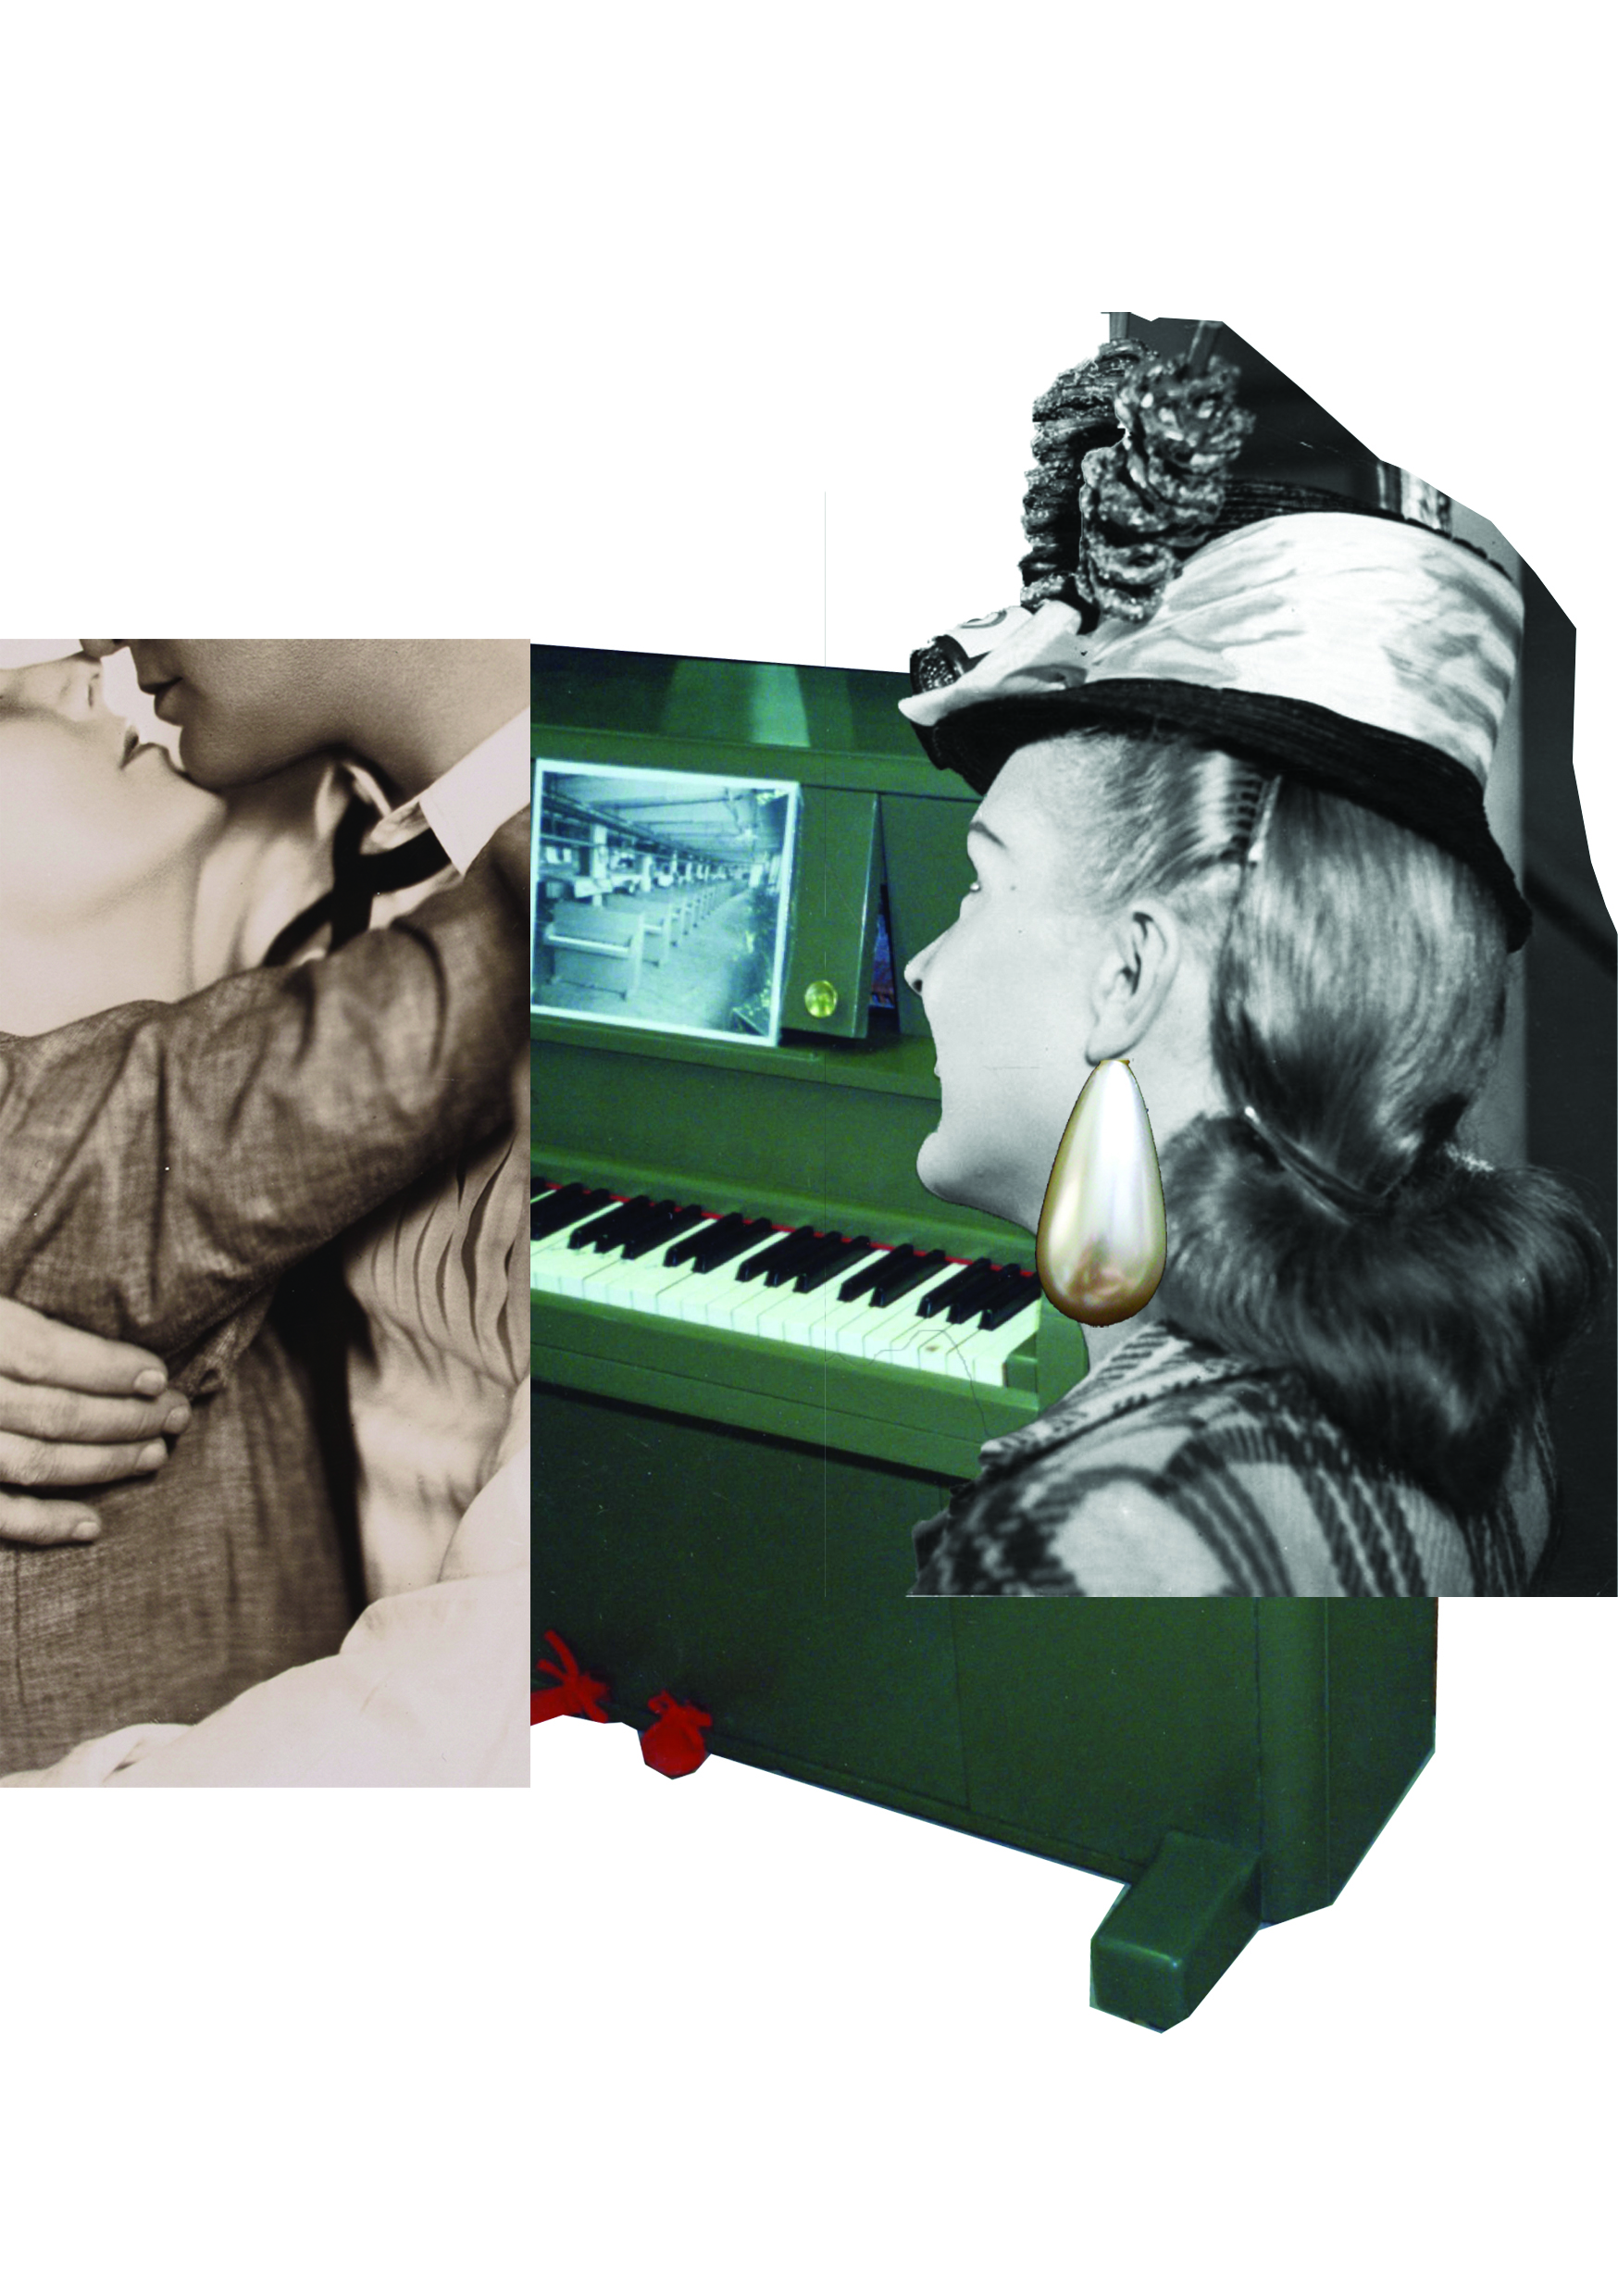
\includegraphics[width=140mm]{../ilustracoes/11_BRINCOS.jpg}
\end{figure}
\pagebreak

\chapterspecial{Os brincos de Sara}{}{Alberto de Oliveira}

\noindent{}De perfil como a via nesse momento, ali no salão, pareceu ao padre
Jerônimo que a cabeça de Sara, a senhora do dr. Romualdo, sob o toque de
luz refletida de cima, tinha qualquer coisa da cabeça das antigas judias
de vastos cabelos de um louro de searas ao sol. Via-a com bons olhos o
padre e não era a miúdo, era agora que ao pé da janela, onde ficara,
recebendo a fresca da noite, suspendia-se a conversação com a entrada de
duas senhoras, vizinhas provavelmente, que acudiam à pequena festa
familiar em casa do honrado coletor de rendas Pereira Nonato, por cuja
fronte um ano mais e admiradores e amigos vinham desfolhar as rosas e as
sentenças do estilo. A cabeça era realmente formosa, digna de inspirar
verdadeiros rasgos de pena, ou pincel, se houvesse artistas nessa pobre
cidade do interior e pelo tempo em que isto se dá.

Padre Jerônimo tinha descido os olhos do alto, do opulento toucado, onde
notara um cambiar de reflexos de diamantes, e contornava agora o nácar
da orelha, nua, junto à qual, numa estriga de ouro abandonada, brincavam
os raios da luz. Devia ser uma pérola aquele pingo lácteo e brilhante
que lá estava pendente do lobo --- faltava-lhe a irmã, não a podia ver,
mas a adivinhava, caindo do outro lado, da mesma altura, igual como
iguais eram os orelhas que os suspendiam.

Com que fim foram inventados os brincos?\ldots{} As damas, tanto as antigas
como as modernas, lera em Plínio, costumam trazer arrecadas pelo prazer
de ouvir o soído leve de suas pérolas junto do ouvido. Mas S. Francisco
de Sales, na \emph{Vida} \emph{Devota}, diz que Isaac, o grande amigo de
Deus, enviara um desses mimos com arras de seu amor à casta Rebeca, de
onde conclui que esse ornamento místico significa que a primeira coisa
que um marido deve alcançar da mulher, e que esta lhe deve fielmente
guardar, é o ouvido, para que nenhum rumor ou linguagem aí penetre,
senão o amável murmúrio das castas e pudicas palavras que são as pérolas
orientais do Evangelho\ldots{}

--- Está triste, padre?

--- Ah! Distraíra-me\ldots{}

A pérola ficou um instante sem o miramento dos olhos do padre Jerônimo.
A conversação reatara-se. Falava-se de política --- aproximavam-se as
eleições. Pereira Nonato esboçava a fisionomia do candidato da oposição.

--- Vocês o conhecem, raso como uma calçada! Formou-se, é verdade, é
doutor, doutor na asneira, como já ouvi dizer de um. Incapaz de
sustentar uma discussão, incapaz de abrir a boca que não diga tolice,
que irá ele fazer na Câmara, na hipótese de ser eleito?

--- Qual eleito! Tão certo como ser hoje o dia que é, será derrotado!

--- Homem, sempre tenho cá meu receio\ldots{}

Vozes protestaram:

---Não alcança cem votos!

--- Cem? Não alcança vinte!

--- Será derrotado!

Romualdo era o candidato oficial. Falou-se de suas virtudes, de seu tino
político, de sua capacidade. Um dos da roda, Argemiro Barbosa,
bradava:\footnote{bradar: gritar.}

--- Há de ser ele o eleito! Há de ser eleito o dr. Romualdo!

Ouvindo nomear o marido, Sara voltou-se na cadeira onde se achava
sentada. A pérola que estava do outro lado, a que o padre Jerônimo não
tinha podido ver, mas adivinhava, caindo da mesma altura, igual como
iguais eram as orelhas que as suspendiam, a ela e à irmã, surgiu desta
vez aos seus olhos, saltando leve sob o pequeno lobo de nácar. Não eram
as castas e pudicas palavras da Santa Escritura que andavam na sala, mas
era o nome do dr. Romualdo. E padre Jerônimo achou natural que Sara
voltasse a cabeça, natural mesmo que pregasse agradecida aquele par de
olhos negros na figura tesa de Argemiro Barbosa, que, enfiada a mão na
cava do colete, repetia profético:

--- Não tem que ver, há de ser eleito o dr. Romualdo!

Mas chegaram novas visitas: o Torres com a filha, o Lima da agência de
correio, os dois Barros, a família Moreira, três senhoras acompanhadas
de um rapaz gordo, o Moreirinha, muito baixo, achaparrado de corpo.
Nonato adiantara-se para a porta e, todo inclinado, ia recebendo as
felicitações. O salão animava-se. Aqui, ali, formavam-se grupos. Caras
de criados irrompiam do corredor, espiando. De fora, pelas janelas
abertas, entrava o ar da noite, impregnado de um cheiro de jasmins e de
trepadeiras.

Súbito fez-se ouvir o piano e houve um remeximento geral no salão.
Ensaiava-se o baile. Padre Jerônimo deu por falta de Argemiro Barbosa;
relanceou os olhos e foi descobri-lo sentado ao pé de Sara,
segredando-lhe alguma coisa ao ouvido. Sara sorriu. Não eram certamente
as castas e pudicas palavras de que fala a \emph{Vida} \emph{Devota},
eram outras, manobras eleitorais, ou coisa que as valha. Modificação
necessária dos tempos. A pérola, pois só se via uma, encoberta como
estava a outra pelo queixo de Argemiro, dançava à ponta da orelha de
nácar,\footnote{nácar: cor ou tom rosado.} às risadinhas de Sara, como
justificando a opinião exarada em Plínio.

Mas ao lado, na outra janela, cochichavam duas senhoras; eram as
Moreiras, duas quarentonas que, segundo elas mesmas diziam, teimavam em
ser solteiras, praguejando horrores contra o casamento, como calamidade
que é. Padre Jerônimo ouviu de uma a palavra ``escândalo'', dita com
ênfase, e desviou os olhos das arrecadas e dos olhos de Sara.

--- Escândalo! A cidade está cheia dessa pouca vergonha!

E a outra Moreira:

--- Sei lá, nhá Angana! Há tanta intriga por este mundo!

Que pouca vergonha seria essa a que se referira a Feliciana Moreira?
Padre Jerônimo aguçou o ouvido, mas era tarde, e a pianista, uma senhora
de óculos, muito pálida e de longos dedos marmóreos e esguios, deu o
sinal para a primeira quadrilha. Ergueram-se os pares, mas ao menino
tempo, do lado de fora, junto à porta, irrompeu violenta algazarra, em
que se ouviam protestos e vozes de injúria. Ameaçava-se:

--- Racho-o! Ignorante é você!

Nonato, que acudira ao tumulto, pacificava:

--- Que é isso, senhores? Mas que vem a ser isso? Calma!

Outros homens chegaram. Soube-se logo: uma questão política entre o
Torres e o Moreirinha. Aquele exaltava os méritos do dr. Romualdo e este
os do candidato da oposição. Daí o barulho. Mas o culpado era o
Moreirinha; não se insulta assim, sem mais nem menos, a um homem de
prestígio, como o dr. Romualdo. Aqui a requesta pareceu reacender-se de
novo:

--- Não insultei ninguém. Foi de você que partiu a afronta.

--- Insultou. Esse é vezo seu muito antigo.

--- Ora, cale-se!

--- Cale-se, não! Quem é você para me obrigar a calar?

---Bem, meus senhores, está acabado, está acabado. Dê-me seu braço, sr.
Moreirinha.

Satisfeito por haver acalmado o distúrbio, Nonato afastou-se, tendo ao
lado o valente oposicionista. Do salão algumas senhoras tinham recuado
assustadas, enfiando-se pelo corredor. Um ou outro cavalheiro
tranquilizava-as. Padre Jerônimo, que chegara até à porta para saber o
que havia, voltara ao fim de alguns minutos, resolvido a pedir o chapéu
e retirar-se. Demais, eram horas; consultara o relógio. O chapéu estava
num quarto, à direita, com os dos demais convidados. Lembrou-lhe, como
melhor, não pedi-lo, mas ir pessoalmente buscá-lo. Adiantou-se. A porta
achava-se meio fechada, impeliu-a. À luz que vinha da sala, dois vultos
depararam-se-lhe à frente: um homem e uma senhora. O homem era Argemiro
Barbosa.

--- Procura seu chapéu, reverendo? Então já se vai? Olhe, deve ser este,
aqui está.

--- Obrigado.

Nessa noite, em casa, ao deitar-se, padre Jerônimo não pôde resistir à
tentação de pensar alguns minutos nas formosas pérolas que a mulher de
Romualdo trazia às orelhas. E a passagem de São Francisco de Sales
acudiu-lhe de novo. A primeira coisa que um marido deve alcançar da
mulher, e que esta lhe deve fielmente guardar, é o ouvido, para que
nenhum rumor ou linguagem aí penetre, senão o amável murmúrio das castas
e pudicas palavras que são as pérolas orientais do Evangelho.

\pagebreak
\thispagestyle{empty}
\begin{figure}
\vspace*{-.5cm}
\hspace*{-2.3cm}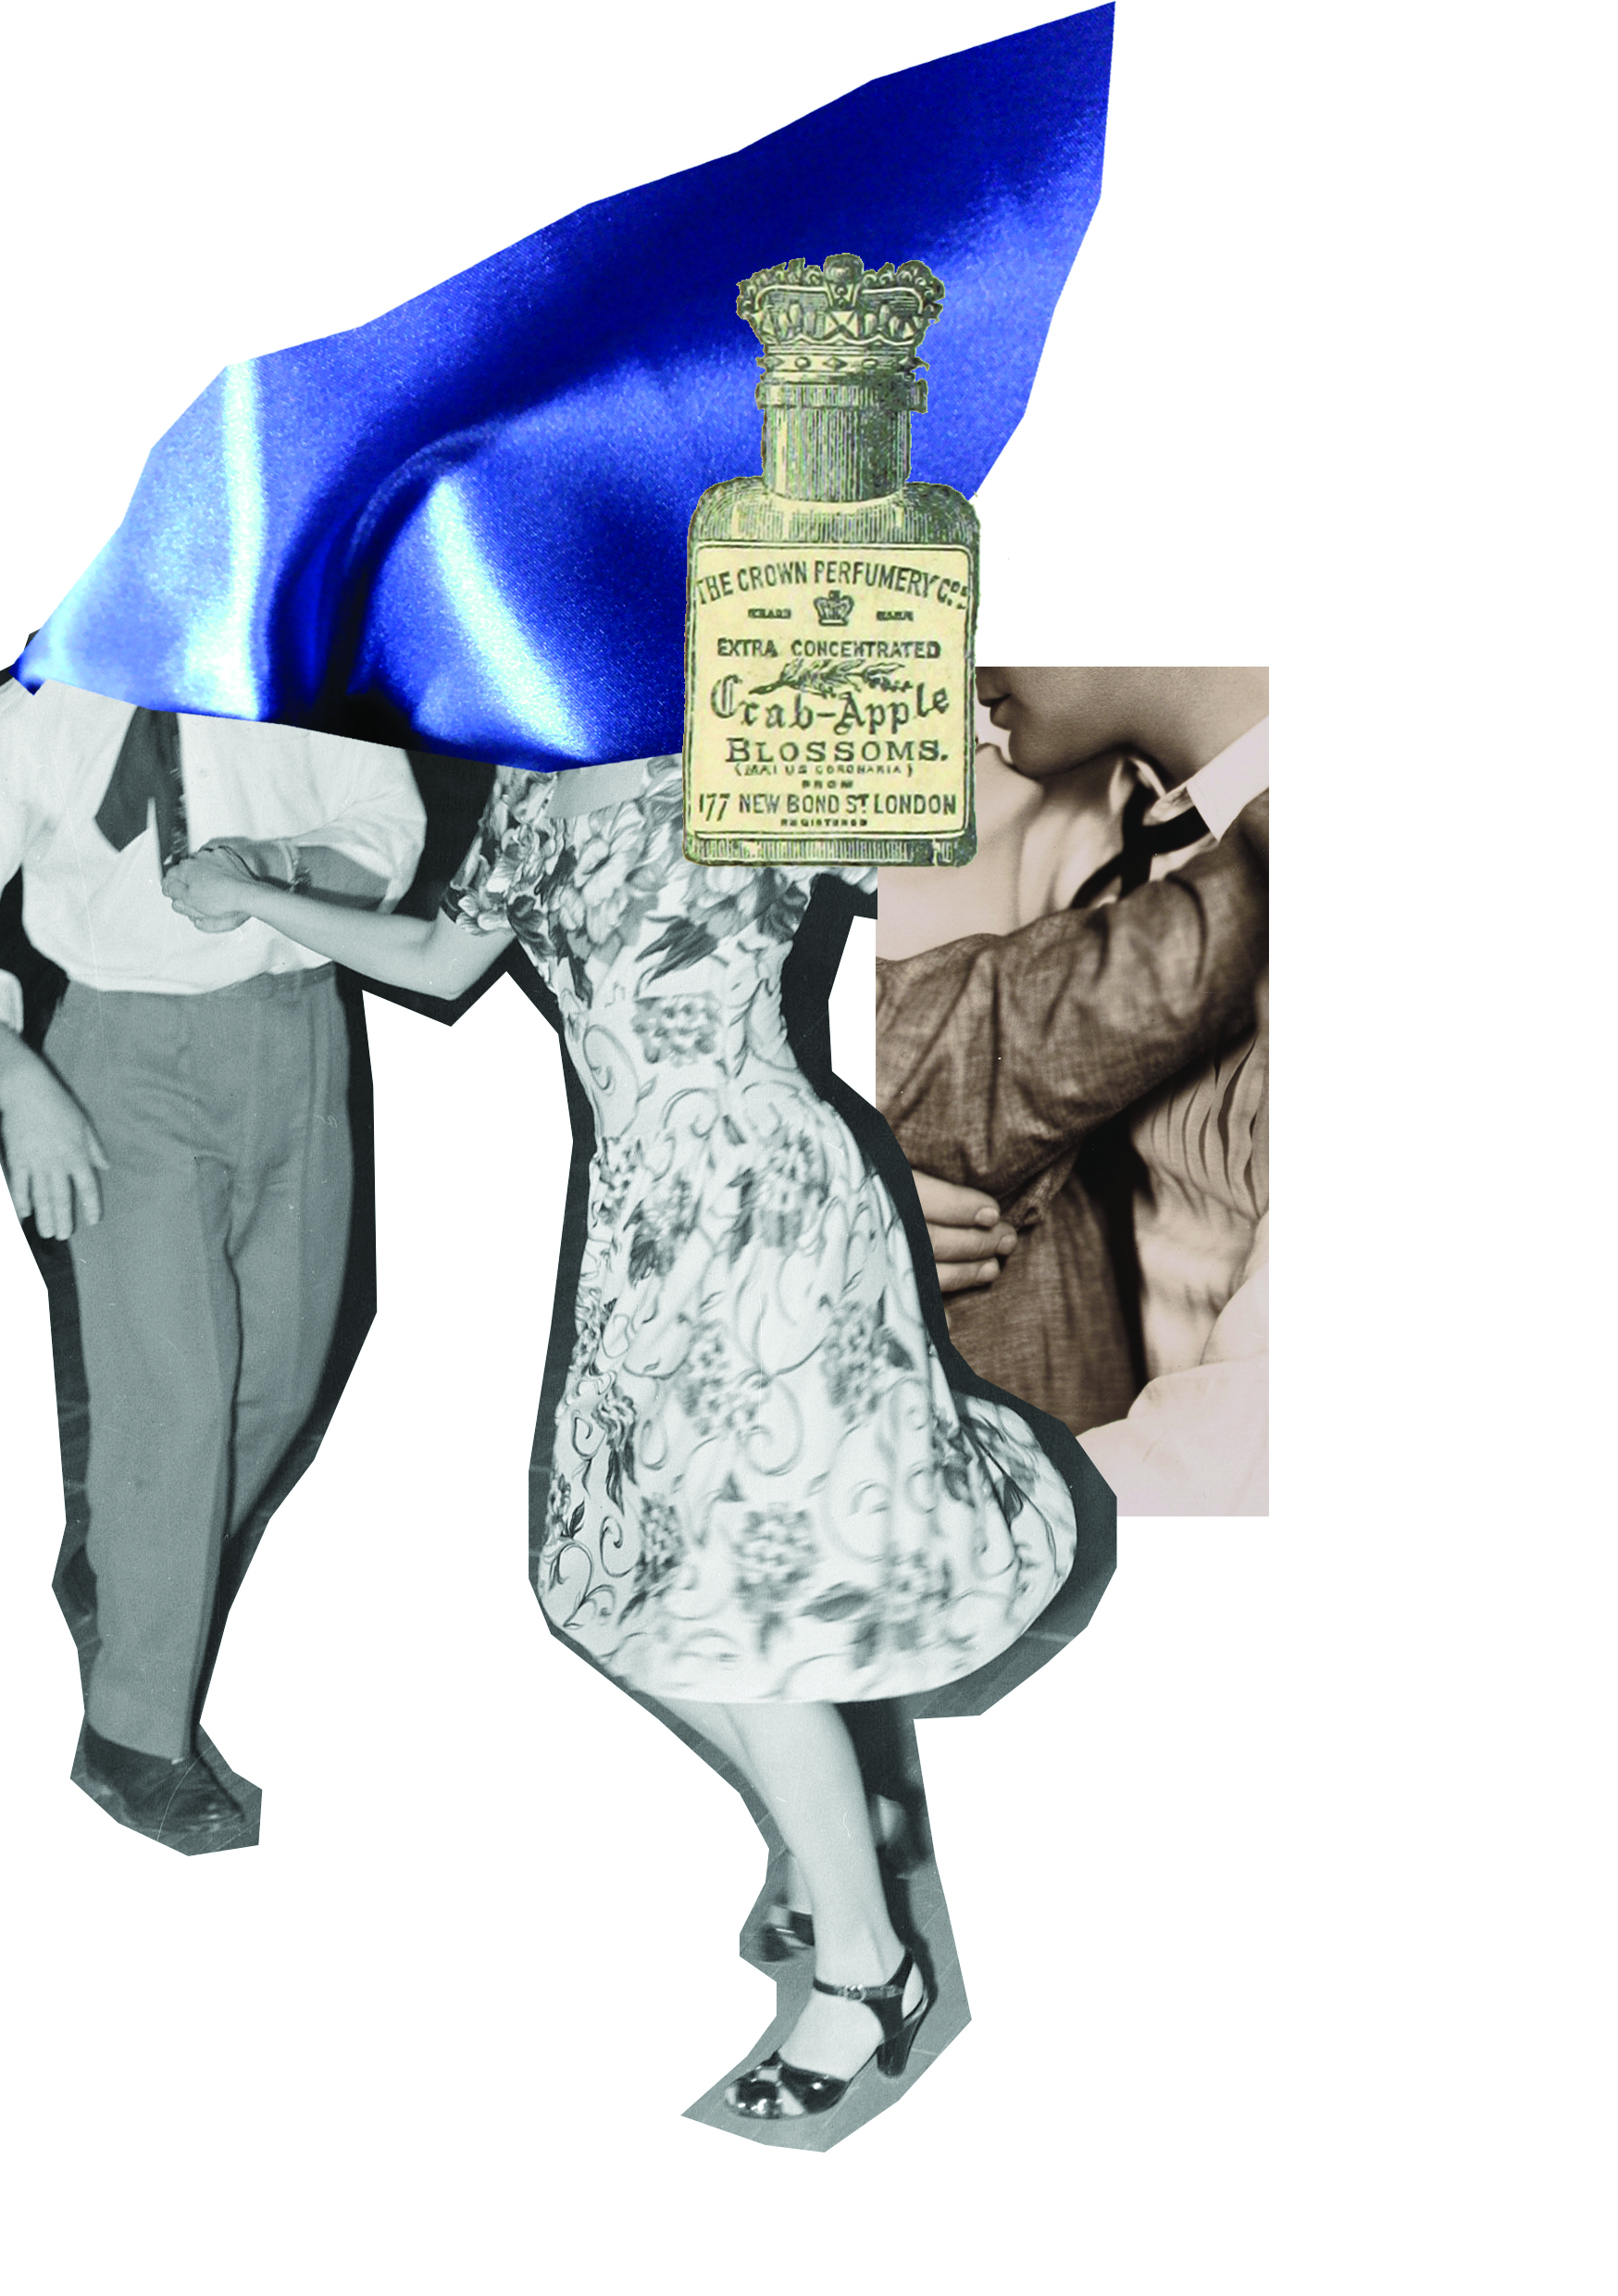
\includegraphics[width=140mm]{../ilustracoes/12_UTIL.jpg}
\end{figure}
\pagebreak

\chapterspecial{Útil inda brincando}{}{Artur Azevedo}

\begin{flushright}
\emph{A Urbano Duarte}
\end{flushright}

\section{I}

Uma noite o Leopoldo das Neves encontrou no Passeio Público o Viriato
Lopes, o Viriatinho da Estrada de Ferro, um bom camarada que há muito
tempo não via.

E, como os dous amigos se encaminhassem para o terraço, o Viriatinho
chamou a atenção do outro para uma bonita mulher que descia a escada em
companhia de um sujeito gordo.

--- Oh, diabo! é a Clotilde! exclamou o Leopoldo das Neves.

E, levando o amigo pelo braço, embarafustou pela sombria alameda que
contorna o lago.

--- Que é isso? Foges daquella mulher?

--- Como o diabo da cruz!

--- Por quê?

--- Porque me amola; se me visse, eu seria amanhã obrigado a
explicar-lhe por miúdo o que vim fazer ao Passeio Público!

--- Amola-te? Ora essa! Eis aí o caso de dizer que dá Deus nozes\ldots{}

--- Perdão, tenho muito bons dentes!

--- Nesse caso, és difícil!

--- A Clotilde não é o meu tipo.

--- Pois é bonita como seiscentos diabos!

--- Não nego; mas o meu ideal é outro. Quisera que a minha amante fosse
alta, magra, loura, alva, de olhos azuis, e tivesse vinte e quatro anos,
quando muito. Quisera também que fosse viúva, conhecesse um pouco a
Europa, e, sem ser literata nem artista, gostasse das lettras e das
artes.

--- Quiseras muita coisa junta!

--- A Clotilde é o contrário de tudo isso: é mais baixa que alta, é mais
gorda que magra, é morena, tem olhos castanhos, e já completou a idade
exigida para a senatoria\ldots{}

--- Do Império?

--- Não; da República. --- É a digna esposa daquele negociante anafado e
suarento que viste passar; adormece no Lírico ouvindo o \emph{Otelo}; dá
o cavaquinho pelos cromos de Guimarães Ferdinando, e delicia-se com a
leitura de Xavier de Montépin, --- traduzido, note-se, porque nem ao
menos sabe francês!\ldots{}

--- E as tuas relações com ela têm tido caráter platônico\ldots{} ou\ldots{}
positivo?

--- Ah, meu amigo, eu dei-lhe, infelizmente, amplo direito de
perseguir-me\ldots{}

--- Maganão!

--- Quem principiou fui eu. Que queres?\ldots{} a curiosidade\ldots{} o vício
\ldots{} a poesia do adultério\ldots{} Como isso foi? Não sei. Um encontro numa
\emph{soirée}\footnote{\emph{soirée}: reunião social que acontece à
  noite.} familiar\ldots{} um aperto de mão mais forte\ldots{} uma valsa\ldots{}
durante a valsa uma troca de lenços\ldots{} no lenço dela um perfume
capitoso\footnote{capitoso: inebriante.} e enervante\ldots{} uma carta minha
que ficou sem resposta\ldots{} outra\ldots{} outra ainda\ldots{} outra, que foi
respondida afinal\ldots{} uma entrevista concedida depois de uma luta
homérica entre duas fomes de beijos\ldots{}

--- Bonito!

--- Uma entrevista em casa de uma cartomante da rua da Assembleia\ldots{}
Duas horas de prazer, e quatro anos de cativeiro e arrependimento!

--- Quatro anos?

--- Sim, meu Viriatinho, há quatro anos que isto dura; há quatro anos
hipotequei a minha liberdade, o meu sossego e o meu bom humor; há quatro
anos vivo aguilhoado a essa mulher, que se encontra comigo de oito em
oito, de quinze em quinze dias, furtivamente, às pressas, mas que me
escreve todos os dias, e me atormenta com protestos, exigências,
lamúrias, ameaças!\ldots{}

E Leopoldo das Neves interrompeu a lista das impertinências de Clotilde,
batendo violentamente com a bengala na relva:

--- Quatro anos! Há quatro anos --- calcula! --- tenho o coração nas
mãos, receoso que de um momento para outro o marido descubra tudo,
ponha-a na rua a pontapés, e eu seja obrigado a ficar com aquela trouxa
às costas!\ldots{}

--- Vejo que já não a amas.

--- Nem nunca a amei. Foi um capricho\ldots{} Quinze dias depois da nossa
primeira entrevista em casa da cartomante, já eu me sentia farto e
aborrecido!

Os dois amigos encaminharam-se para o terraço.

A noite estava esplêndida. Não havia luar, mas os astros brilhavam
intensamente na profunda escuridão do céu. As ondas, derramando-se na
praia, pareciam alvíssimas rendas franjando uma enorme colcha azul.

Queres um conselho, Viriatinho? Foge das ligações dessa espécie.

--- Ah! de que me serve o teu conselho?

--- Por quê?

--- Aqui onde me vês estou ralado de inveja!

--- De inveja?

--- Sim, confesso-te que surprendo cá dentro esse sentimento ignóbil.
Invejo a perseguição de que te dizes vítima, e --- palavra ! --- tenho
ciúmes, ciúmes incoerentes, dessa mulher que não é minha, que não
conheço, que apenas entrevi\ldots{} Eu dava dez annos de vida --- vê tu lá!
--- pelo prazer de entrar com ela, furtivamente, em casa de uma
cartomante misteriosa e hospitaleira!

Leopoldo das Neves encarou fixamente o outro, e, depois de uma grande
pausa, perguntou-lhe, segurando-o por um botão do casaco:

--- Viriatinho, és meu amigo?

--- Certamente.

--- Queres prestar-me um grande serviço ?

--- Qual?

--- Um serviço que não te será desagradavel?

--- Que ordenas tu?

O amante de Clotilde recuou dous passos, apontou para o lado da rua, e
declamou o verso de D. Salústio:

\emph{De plaire à cette femme et d'être son amant!}\footnote{\emph{De
  plaire à cette femme et d'être son amant!}: De agradar a esta mulher e
  de ser seu amante!}

O Viriatinho soltou uma gargalhada tão cristalina e vibrante, que chamou
a atenção das pessoas que passavam.

--- Não te rias! estou falando sério!\ldots{}

--- Mas isso é lá possível! Tirar-te do lance, eu!\ldots{} E ela tão
apaixonada por ti!\ldots{}

--- Conheço-a como as palmas das minhas mãos; dar-te-ei as instruções
necessárias\ldots{} Desde que estejas munido de todos os recursos
estratégicos, desde que saibas como atacar a praça, a vitória não será
difficil.

--- Olha que sou um péssimo general!

--- Deixa-te de modéstias! Vamo-nos embora\ldots{} Pelo caminho irei te
desenvolvendo o plano do ataque.

--- Vamos lá!

Os dous amigos tomaram a direção da escada.

--- Não calculas como vais ser útil! disse Leopoldo das Neves, descendo.

--- ``Útil inda brincando'', acrescenlou Viriatinho, descendo também, e
apontando para o desgracioso Cupido que desde 1783 dá de beber aos
fluminenses.

\section{II}

Mês e meio depois desse encontro no Passeio Público, Leopoldo das Neves
estava sozinho em casa, e sentia um aborrecimento de morte.

Era uma noite chuvosa e fria.

Tentou escrever, e não conseguiu alinhar quatro palavras; quis ler um
livro interessante, que ainda não conhecia, e fechou o volume logo
depois da segunda página; sentou-se ao piano, e sentiu as mãos pesadas
como se fossem de chumbo. Acendeu um charuto, e deitou-se na cama a fio
comprido, contemplando os bicos dos pés.

Tinham-se já passado quarenta dias depois que ele apresentara Viriatinho
a Clotilde, numa \emph{soirée}, em casa de um tal comendador Freixo.

Leopoldo tratara Clotilde com muita indiferença, passando a noite a
jogar o voltarete com o marido dela, um major de engenheiros e um
médico. De vez em quando o Viriatinho lhe apparecia na sala do jogo, e,
por gestos, o informava de que tudo corria às mil maravilhas.

Terminada a \emph{soirée}, os dois amigos saíram juntos e, na rua, deram
cinquenta passos ao lado um do outro, sem se falar.

Leopoldo quebrou o silêncio:

--- Então, César? Chegaste, viste e venceste?

Por única resposta o Viriatinho tirou da algibeira um pequenino lenço e
apresentou-o a Leopoldo, dizendo:

--- Vê se conheces este perfume.

--- Bravo!\ldots{} as coisas chegaram à cerimônia, meio maometana, da troca
dos lenços?

--- Tal qual como comtigo. Primeiro que tudo, e modéstia à parte, não há
dúvida que lhe fiz certa impressão. É que naturalmente me achou parecido
com algum herói de Xavier de Montépin. O resto já tu sabes: uns olhares
ardentes e expressivos\ldots{} uns apertos de mão durante a primeira
quadrilha\ldots{} logo em seguida uma valsa, e a troca dos lenços\ldots{} Depois
de amanhã lhe escreverei uma carta\ldots{}

Os dous amigos separaram-se, e, desde essa ocasião, Leopoldo não mais
esteve com o Viriatinho.

A correspondência de Clotilde cessou completamente.

Durante os primeiros dias ele sentiu-se feliz, aliviado --- uf! ---
daquela pesada algema que durante quatro anos penosamente arrastara.
Depois vieram-lhe\ldots{} como direi?\ldots{} remorsos. Recordava-se do passado;
saudosas cenas se renovavam no seu cérebro inquieto.

Clotilde aparecia-lhe agora com toda a sua meiguice, com todo o seu
ardor de mulher que fecha os olhos e se entrega resolutamente a um
homem, como se mergulhasse no oceano.

Depois, ele passou noites consecutivas a sonhar com ela: via-a muito
alta, muito magra, muito loura, de olhos azuis, a tocar harpa,
dizendo-lhe:

--- Aqui me tens! Agora, sim, agora sou o teu ideal!\ldots{}

Naquella noite chuvosa e úmida, Leopoldo sentia-se mais do que nunca
envergonhado do seu procedimento. Por fim de contas, Clotilde era uma
bonita mulher, e uma boa rapariga, que só tivera um defeito: amá-lo
exageradamente. E que fez ele? Uma canalhice: entregou-a ao Viriatinho,
ao Viriatinho da Estrada de Ferro, um pulha, uma besta que com certeza
não saberia apreciá-la!\ldots{}

O ingrato monologava esta interrogação terrível:

--- Já teriam ido à rua da Assembleia? ---, quando ouviu bater à porta.

Foi abrir. Era o Viriatinho, que entrou alegre e radiante.

--- Está chovendo: tinha certeza de encontrar-te em casa. Venho
trazer-te notícias da minha conquista\ldots{} Fomos hoje à
cartomante!\ldots{}

Leopoldo estremeceu, teve um sorriso contrafeito, e agarrou-se a um
móvel para não cair.

--- Apre! Custou! Escrevi-lhe nada menos de seis cartas! As três
primeiras ficaram sem resposta. Afinal, foi ela própria quem me indicou
o \emph{buen retiro} da rua da Assembleia\ldots{} Talvez o mesmo quarto,
heim? ·

--- Talvez\ldots{}

--- Olha: sobem-se duas escadas\ldots{} abre-se uma grade de pau\ldots{} entra-se
num corredor\ldots{} primeira alcova\footnote{alcova: aposento; quarto de
  casal.} à direita\ldots{} com uma janela que dá para uma área\ldots{} Embaixo
uma casa de fumos\ldots{} É isso?\ldots{}

As palavras do Viriatinho penetravam no coração de Leopoldo das Neves
como outras tantas punhaladas.

O pobre-diabo teve impelos de agarrar numa bengala, e pôr pela porta
fora, a pauladas, o seu substituto ; mas --- que diabo ! --- o culpado
de tudo não tinha sido ele próprio?\ldots{} ele próprio não lhe indicara os
meios de seduzir Clotilde?\ldots{} não era esse o resultado fatal de uma
combinação infame, proposta espontaneamente por ele?

O Viriatinho observou:

--- Mas\ldots{} valha-me Deus! acho-te assim a modo que contrariado\ldots{} Estás
arrependido?

--- Eu?\ldots{} que ideia!\ldots{} murmurou Leopoldo sufocado; que ideia!\ldots{}

--- Olha, se queres que te diga, acho que tinhas muita razão\ldots{} A
Clotilde é bonita, isso é, mas que mulher vulgar! que espírito
acanhado!\ldots{} Não tem por onde se lhe pegue!\ldots{}

--- Não te dizia? acudiu vivamente Leopoldo, regozijado por essa
opinião; a Clotilde não vale nada!

--- Sabes? não estou disposto a aguentar aquilo quatros anos, como tu\ldots{}
Nada! na primeira ocasião desfaço-me dela! Quis apenas prestar-te um
serviço, e folgo de ter sido ``útil inda brincando''.

Alguns minutos depois, o Viriantinho saiu, e Leopoldo das Neves ficou
aniquilado pelo desgosto.

Foi para o seu quarto de dormir, abriu um armário, e tirou um vidro de
perfumaria, o extrato predileto de Clotide, há três anos esquecido no
fundo daquele móvel. Ensopou o lenço, aspirou longamente aquele perfume
``capitoso e enervante'' como se quisesse anestesiar-se; depois,
atirou-se à cama, enterrou a cabeça no travesseiro, e numa crise de
nervos, começou a chorar desesperadamente, soluçando o nome dela.

Passou assim toda a noite.

Ela enviuvou há um ano. Eles casaram-se há seis meses.

Quando se encontram com o Viriatinho da Estrada de Ferro, fingem que o
não conhecem.

\pagebreak
\thispagestyle{empty}
\begin{figure}
\vspace*{-.5cm}
\hspace*{-2.3cm}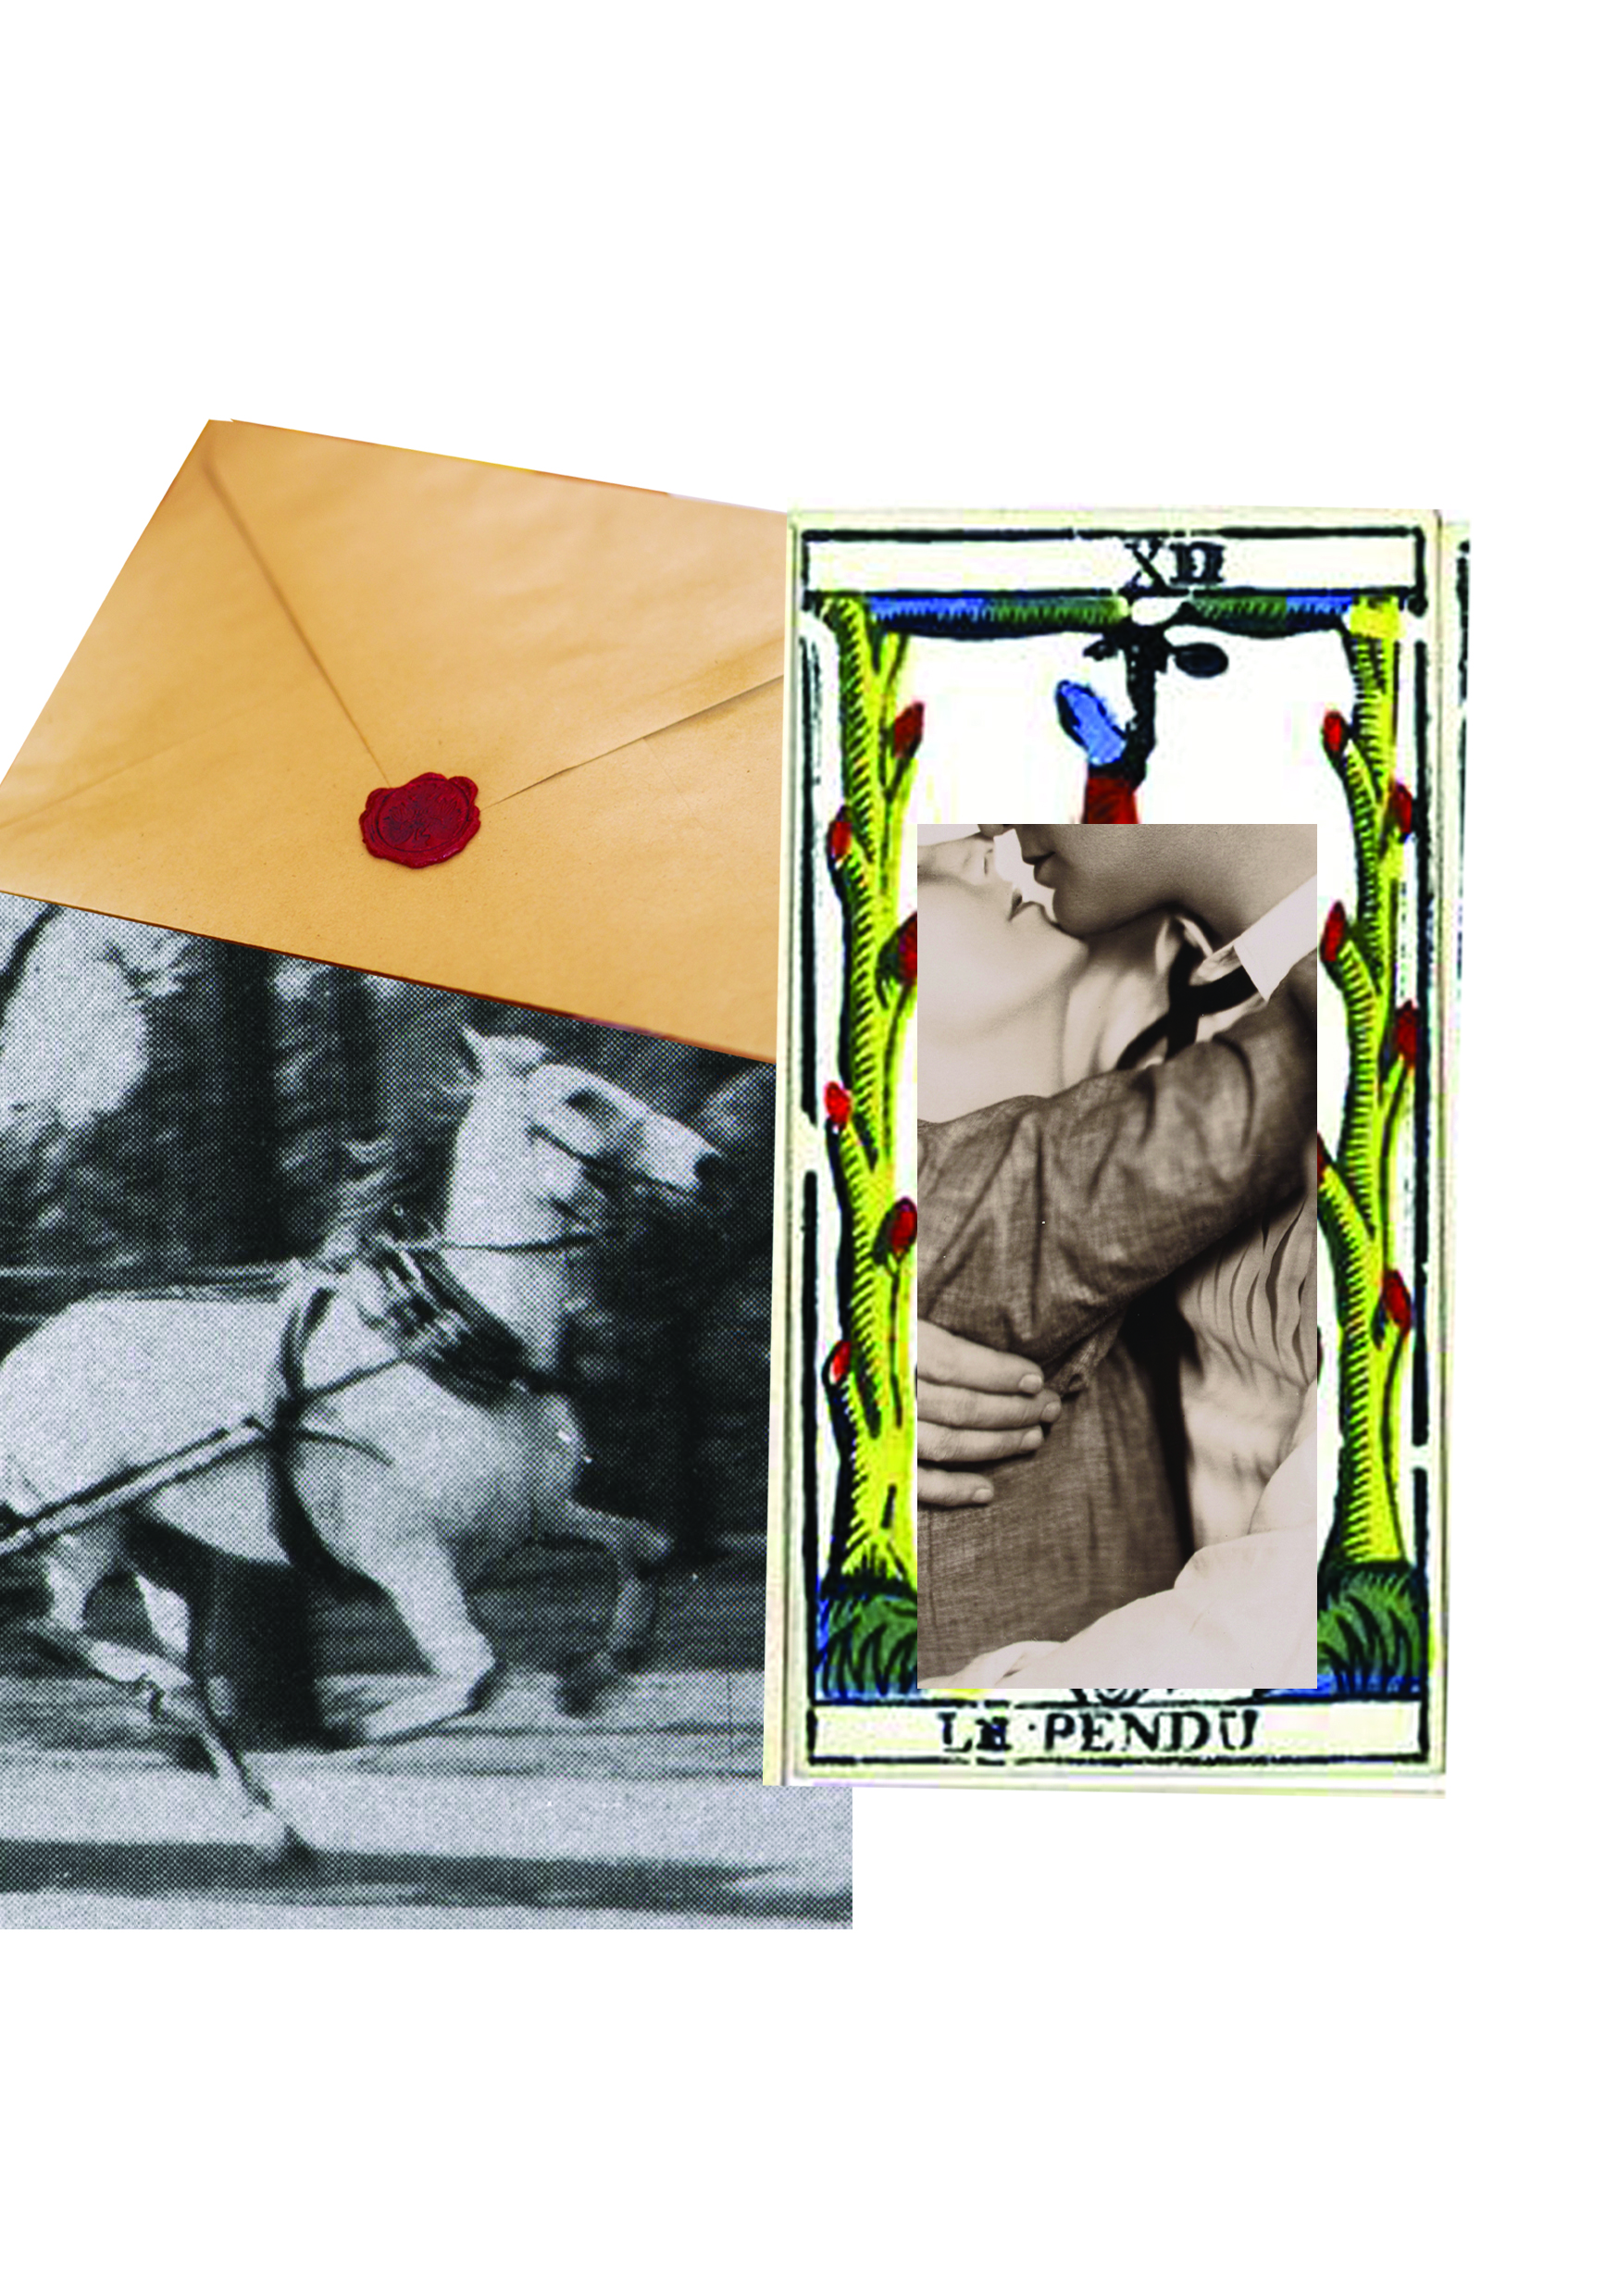
\includegraphics[width=140mm]{../ilustracoes/13_CARTOMANTE.jpg}
\end{figure}
\pagebreak

\chapterspecial{A cartomante}{}{Machado de Assis}

\noindent{}Hamlet observa a Horácio\footnote{Hamlet, Horácio: personagens da peça
  teatral \emph{Hamlet}, de William Shakespeare (1564--1616).} que há
mais coisas no céu e na terra do que sonha a nossa filosofia. Era a
mesma explicação que dava a bela Rita ao moço Camilo, numa sexta-feira
de novembro de 1869, quando este ria dela, por ter ido na véspera
consultar uma cartomante; a diferença é que o fazia por outras palavras.

--- Ria, ria. Os homens são assim; não acreditam em nada. Pois saiba que
fui, e que ela adivinhou o motivo da consulta, antes mesmo que eu lhe
dissesse o que era. Apenas começou a botar as cartas, disse-me: ``A
senhora gosta de uma pessoa\ldots''. Confessei que sim, e então ela
continuou a botar as cartas, combinou-as, e no fim declarou-me que eu
tinha medo de que você me esquecesse, mas que não era verdade\ldots{}

--- Errou! --- interrompeu Camilo, rindo.

--- Não diga isso, Camilo. Se você soubesse como eu tenho andado, por
sua causa. Você sabe; já lhe disse. Não ria de mim, não ria\ldots{}

Camilo pegou-lhe nas mãos, e olhou para ela sério e fixo. Jurou que lhe
queria muito, que os seus sustos pareciam de criança; em todo o caso,
quando tivesse algum receio, a melhor cartomante era ele mesmo. Depois,
repreendeu-a; disse-lhe que era imprudente andar por essas casas. Vilela
podia sabê-lo, e depois\ldots{}

--- Qual saber! Tive muita cautela, ao entrar na casa.

--- Onde é a casa?

--- Aqui perto, na~rua da Guarda Velha; não passava ninguém nessa
ocasião. Descansa; eu não sou maluca.

Camilo riu outra vez:

--- Tu crês deveras nessas coisas? --- perguntou-lhe.

Foi então que ela, sem saber que traduzia Hamlet em vulgar, disse-lhe
que havia muita coisa misteriosa e verdadeira neste mundo. Se ele não
acreditava, paciência; mas o certo é que a cartomante adivinhara tudo.
Que mais? A prova é que ela agora estava tranquila e satisfeita.

Cuido que ele ia falar, mas reprimiu-se. Não queria arrancar-lhe as
ilusões. Também ele, em criança, e ainda depois, foi supersticioso, teve
um arsenal inteiro de crendices, que a mãe lhe incutiu e que aos vinte
anos desapareceram. No dia em que deixou cair toda essa vegetação
parasita, e ficou só o tronco da religião, ele, como tivesse recebido da
mãe ambos os ensinos, envolveu-os na mesma dúvida, e logo depois em uma
só negação total. Camilo não acreditava em nada. Por quê? Não poderia
dizê-lo, não possuía um só argumento; limitava-se a negar tudo. E digo
mal, porque negar é ainda afirmar, e ele não formulava a incredulidade;
diante do mistério, contentou-se em levantar os ombros, e foi andando.

Separaram-se contentes, ele ainda mais que ela. Rita estava certa de ser
amada; Camilo não só o estava, mas via-a estremecer e arriscar-se por
ele, correr às cartomantes, e, por mais que a repreendesse, não podia
deixar de sentir-se lisonjeado. A casa do encontro era na antiga~rua dos
Barbonos, onde morava uma comprovinciana de Rita. Esta desceu pela rua
das Mangueiras, na direção de Botafogo, onde residia; Camilo desceu pela
da Guarda Velha, olhando de passagem para a casa da cartomante.

Vilela, Camilo e Rita, três nomes, uma aventura, e nenhuma explicação
das origens. Vamos a ela. Os dois primeiros eram amigos de infância.
Vilela seguiu a carreira de magistrado. Camilo entrou no funcionalismo,
contra a vontade do pai, que queria vê-lo médico; mas o pai morreu, e
Camilo preferiu não ser nada, até que a mãe lhe arranjou um emprego
público. No princípio de 1869, voltou Vilela da província, onde casara
com uma dama formosa e tonta; abandonou a magistratura e veio abrir
banca de advogado. Camilo arranjou-lhe casa para os lados de Botafogo, e
foi a bordo recebê-lo.

--- É o senhor? --- exclamou Rita, estendendo-lhe a mão. --- Não imagina
como meu marido é seu amigo, falava sempre do senhor.

Camilo e Vilela olharam-se com ternura. Eram amigos deveras. Depois,
Camilo confessou de si para si que a mulher do Vilela não desmentia as
cartas do marido. Realmente, era graciosa e viva nos gestos, olhos
cálidos, boca fina e interrogativa. Era um pouco mais velha que ambos:
contava trinta anos, Vilela, vinte e nove e Camilo, vinte e seis.
Entretanto, o porte grave de Vilela fazia-o parecer mais velho que a
mulher, enquanto Camilo era um ingênuo na vida moral e prática.
Faltava-lhe tanto a ação do tempo, como os óculos de cristal, que a
natureza põe no berço de alguns para adiantar os anos. Nem experiência,
nem intuição.

Uniram-se os três. Convivência trouxe intimidade. Pouco depois morreu a
mãe de Camilo, e nesse desastre, que o foi, os dois mostraram-se grandes
amigos dele. Vilela cuidou do enterro, dos sufrágios\footnote{sufrágio:
  oração pela alma de morto.} e do inventário; Rita tratou especialmente
do coração, e ninguém o faria melhor.

Como daí chegaram ao amor, não o soube ele nunca. A verdade é que
gostava de passar as horas ao lado dela; era a sua enfermeira moral,
quase uma irmã, mas principalmente era mulher e bonita.~\emph{Odor di
femmina}: eis o que ele aspirava nela, e em volta dela, para
incorporá-lo em si próprio. Liam os mesmos livros, iam juntos a teatros
e passeios. Camilo ensinou-lhe as damas e o xadrez e jogavam às noites;
--- ela, mal, --- ele, para lhe ser agradável, pouco menos mal. Até aí
as coisas. Agora a ação da pessoa, os olhos teimosos de Rita, que
procuravam muita vez os dele, que os consultavam antes de o fazer ao
marido, as mãos frias, as atitudes insólitas. Um dia, fazendo ele anos,
recebeu de Vilela uma rica bengala de presente, e de Rita apenas um
cartão com um vulgar cumprimento a lápis, e foi então que ele pôde ler
no próprio coração; não conseguia arrancar os olhos do bilhetinho.
Palavras vulgares; mas há vulgaridades sublimes, ou, pelo menos,
deleitosas. A velha caleça de praça, em que pela primeira vez passeaste
com a mulher amada, fechadinhos ambos, vale o carro de Apolo. Assim é o
homem, assim são as coisas que o cercam.

Camilo quis sinceramente fugir, mas já não pôde. Rita, como uma
serpente, foi-se acercando dele, envolveu-o todo, fez-lhe estalar os
ossos num espasmo, e pingou-lhe o veneno na boca. Ele ficou atordoado e
subjugado. Vexame, sustos, remorsos, desejos, tudo sentiu de mistura;
mas a batalha foi curta e a vitória delirante. Adeus, escrúpulos! Não
tardou que o sapato se acomodasse ao pé, e aí foram ambos, estrada fora,
braços dados, pisando folgadamente por cima de ervas e pedregulhos, sem
padecer nada mais que algumas saudades, quando estavam ausentes um do
outro. A confiança e estima de Vilela continuavam a ser as mesmas.

Um dia, porém, recebeu Camilo uma carta anônima, que lhe chamava imoral
e pérfido, e dizia que a aventura era sabida de todos. Camilo teve medo,
e, para desviar as suspeitas, começou a rarear as visitas à casa de
Vilela. Este notou-lhe as ausências. Camilo respondeu que o motivo era
uma paixão frívola de rapaz. Candura gerou astúcia. As ausências
prolongaram-se, e as visitas cessaram inteiramente. Pode ser que
entrasse também nisso um pouco de amor-próprio, uma intenção de diminuir
os obséquios do marido, para tornar menos dura a aleivosia do ato.

Foi por esse tempo que Rita, desconfiada e medrosa, correu à cartomante
para consultá-la sobre a verdadeira causa do procedimento de Camilo.
Vimos que a cartomante restituiu-lhe a confiança, e que o rapaz
repreendeu-a por ter feito o que fez. Correram ainda algumas semanas.
Camilo recebeu mais duas ou três cartas anônimas, tão apaixonadas, que
não podiam ser advertência da virtude, mas despeito de algum
pretendente; tal foi a opinião de Rita, que, por outras palavras mal
compostas, formulou este pensamento: ---~a virtude é preguiçosa e avara,
não gasta tempo nem papel; só o interesse é ativo e pródigo.

Nem por isso Camilo ficou mais sossegado; temia que o anônimo fosse ter
com Vilela, e a catástrofe viria então sem remédio. Rita concordou que
era possível.

--- Bem --- disse ela; --- eu levo os sobrescritos para comparar a letra
com a das cartas que lá aparecerem; se alguma for igual, guardo-a e
rasgo-a\ldots{}

Nenhuma apareceu; mas daí a algum tempo Vilela começou a mostrar-se
sombrio, falando pouco, como desconfiado. Rita deu-se pressa em dizê-lo
ao outro, e sobre isso deliberaram. A opinião dela é que Camilo devia
tornar à casa deles, tatear o marido, e pode ser até que lhe ouvisse a
confidência de algum negócio particular. Camilo divergia; aparecer
depois de tantos meses era confirmar a suspeita ou denúncia. Mais valia
acautelarem-se, sacrificando-se por algumas semanas. Combinaram os meios
de se corresponderem, em caso de necessidade, e separaram-se com
lágrimas.

No dia seguinte, estando na repartição, recebeu Camilo este bilhete de
Vilela: ``Vem já, já, à nossa casa; preciso falar-te sem demora''. Era
mais de meio-dia. Camilo saiu logo; na rua, advertiu que teria sido mais
natural chamá-lo ao escritório; por que em casa? Tudo indicava matéria
especial, e a letra, fosse realidade ou ilusão, afigurou-se-lhe trêmula.
Ele combinou todas essas cousas com a notícia da véspera.

--- Vem já, já, à nossa casa; preciso falar-te sem demora --- repetia
ele com os olhos no papel.

Imaginariamente, viu a ponta da orelha de um drama, Rita subjugada e
lacrimosa, Vilela indignado, pegando da pena e escrevendo o bilhete,
certo de que ele acudiria, e esperando-o para matá-lo. Camilo
estremeceu, tinha medo: depois sorriu amarelo, e em todo caso
repugnava-lhe a ideia de recuar, e foi andando. De caminho, lembrou-se
de ir a casa; podia achar algum recado de Rita, que lhe explicasse tudo.
Não achou nada, nem ninguém. Voltou à rua, e a ideia de estarem
descobertos parecia-lhe cada vez mais verossímil; era natural uma
denúncia anônima, até da própria pessoa que o ameaçara antes; podia ser
que Vilela conhecesse agora tudo. A mesma suspensão das suas visitas,
sem motivo aparente, apenas com um pretexto fútil, viria confirmar o
resto.

Camilo ia andando inquieto e nervoso. Não relia o bilhete, mas as
palavras estavam decoradas, diante dos olhos, fixas; ou então --- o que
era ainda pior --- eram-lhe murmuradas ao ouvido, com a própria voz de
Vilela. ``Vem já, já, à nossa casa; preciso falar-te sem demora.'' Ditas
assim, pela voz do outro, tinham um tom de mistério e ameaça. Vem, já,
já, para quê? Era perto de uma hora da tarde. A comoção crescia de
minuto a minuto. Tanto imaginou o que se iria passar, que chegou a
crê-lo e vê-lo. Positivamente, tinha medo. Entrou a cogitar em ir
armado, considerando que, se nada houvesse, nada perdia, e a precaução
era útil. Logo depois rejeitava a ideia, vexado de si mesmo, e seguia,
picando o passo, na direção do~largo da Carioca, para entrar
num~tílburi.\footnote{tílburi: carro de duas rodas e dois assentos, com
  capota e sem boleia, puxado por um só animal.} Chegou, entrou e mandou
seguir a trote largo.

``Quanto antes, melhor, pensou ele; não posso estar assim\ldots''

Mas o mesmo trote do cavalo veio agravar-lhe a comoção. O tempo voava, e
ele não tardaria a entestar com o perigo. Quase no fim da~rua da Guarda
Velha, o~tílburi~teve de parar; a rua estava atravancada com uma
carroça, que caíra. Camilo, em si mesmo, estimou o obstáculo, e esperou.
No fim de cinco minutos, reparou que ao lado, à esquerda, ao pé
do~tílburi, ficava a casa da cartomante, a quem Rita consultara uma vez,
e nunca ele desejou tanto crer na lição das cartas. Olhou, viu as
janelas fechadas, quando todas as outras estavam abertas e pejadas de
curiosos do incidente da rua. Dir-se-ia a morada do indiferente~Destino.

Camilo reclinou-se no~tílburi, para não ver nada. A agitação dele era
grande, extraordinária, e do fundo das camadas morais emergiam alguns
fantasmas de outro tempo, as velhas crenças, as superstições antigas. O
cocheiro propôs-lhe voltar a primeira travessa, e ir por outro caminho;
ele respondeu que não, que esperasse. E inclinava-se para fitar a
casa\ldots{} Depois fez um gesto incrédulo: era a ideia de ouvir a
cartomante, que lhe passava ao longe, muito longe, com vastas asas
cinzentas; desapareceu, reapareceu, e tornou a esvair-se no cérebro; mas
daí a pouco moveu outra vez as asas, mais perto, fazendo uns giros
concêntricos\ldots{} Na rua, gritavam os homens, safando a carroça:

--- Anda! agora! empurra! vá! vá!

Daí a pouco estaria removido o obstáculo. Camilo fechava os olhos,
pensava em outras cousas; mas a voz do marido sussurrava-lhe às orelhas
as palavras da carta: ``Vem, já, já\ldots''. E ele via as contorções do
drama e tremia. A casa olhava para ele. As pernas queriam descer e
entrar\ldots{} Camilo achou-se diante de um longo véu opaco\ldots{}
pensou rapidamente no inexplicável de tantas coisas. A voz da mãe
repetia-lhe uma porção de casos extraordinários, e a mesma frase~do
príncipe de Dinamarca reboava-lhe\footnote{reboar: ecoar fortemente.}
dentro: ``Há mais coisas no céu e na terra do que sonha a nossa
filosofia\ldots''. Que perdia ele, se\ldots?

Deu por si na calçada, ao pé da porta; disse ao cocheiro que esperasse,
e rápido enfiou pelo corredor, e subiu a escada. A luz era pouca, os
degraus, comidos dos pés, o corrimão, pegajoso; mas ele não viu nem
sentiu nada. Trepou e bateu. Não aparecendo ninguém, teve ideia de
descer; mas era tarde, a curiosidade fustigava-lhe o sangue, as fontes
latejavam-lhe; ele tornou a bater uma, duas, três pancadas. Veio uma
mulher; era a cartomante. Camilo disse que ia consultá-la, ela fê-lo
entrar. Dali subiram ao sótão, por uma escada ainda pior que a primeira
e mais escura. Em cima, havia uma salinha, mal alumiada por uma janela,
que dava para o telhado dos fundos. Velhos~trastes, paredes sombrias, um
ar de pobreza, que antes aumentava do que destruía o prestígio.

A cartomante fê-lo sentar diante da mesa, e sentou-se do lado oposto,
com as costas para a janela, de maneira que a pouca luz de fora batia em
cheio no rosto de Camilo. Abriu uma gaveta e tirou um baralho de cartas
compridas e enxovalhadas. Enquanto as baralhava, rapidamente, olhava
para ele, não de rosto, mas por baixo dos olhos. Era uma mulher de
quarenta anos, italiana, morena e magra, com grandes olhos sonsos e
agudos. Voltou três cartas sobre a mesa, e disse-lhe:

--- Vejamos primeiro o que é que o traz aqui. O senhor tem um grande
susto\ldots{}

Camilo, maravilhado, fez um gesto afirmativo.

--- E quer saber --- continuou ela --- se lhe acontecerá alguma coisa ou
não\ldots{}

--- A mim e a ela --- explicou vivamente ele.

A cartomante não sorriu; disse-lhe só que esperasse. Rápido pegou outra
vez das cartas e baralhou-as, com os longos dedos finos, de unhas
descuradas;\footnote{descuradas: não cuidadas, não tratadas.}
baralhou-as bem, transpôs\footnote{transpor: mudar de um lugar para
  outro.} os maços, uma, duas, três vezes; depois começou a estendê-las.
Camilo tinha os olhos nela, curioso e ansioso.

--- As cartas dizem-me\ldots{}

Camilo inclinou-se para beber uma a uma as palavras. Então ela
declarou-lhe que não tivesse medo de nada. Nada aconteceria nem a um nem
a outro; ele, o terceiro, ignorava tudo. Não obstante, era indispensável
muita cautela: ferviam invejas e despeitos. Falou-lhe do amor que os
ligava, da beleza de Rita\ldots{} Camilo estava deslumbrado. A
cartomante acabou, recolheu as cartas e fechou-as na gaveta.

--- A senhora restituiu-me a paz ao espírito --- disse ele estendendo a
mão por cima da mesa e apertando a da cartomante.

Esta levantou-se, rindo.

--- Vá --- disse ela ---; vá,~\emph{ragazzo innamorato}\ldots{}

E de pé, com o dedo indicador, tocou-lhe na testa. Camilo
estremeceu,~como se fosse a mão da própria sibila, e levantou-se também.
A cartomante foi à cômoda, sobre a qual estava um prato com passas,
tirou um cacho destas, começou a despencá-las e comê-las, mostrando duas
fileiras de dentes que desmentiam as unhas. Nessa mesma ação comum, a
mulher tinha um ar particular. Camilo, ansioso por sair, não sabia como
pagasse; ignorava o preço.

--- Passas custam dinheiro --- disse ele afinal, tirando a carteira. ---
Quantas quer mandar buscar?

--- Pergunte ao seu coração --- respondeu ela.

Camilo tirou uma nota de dez mil-réis, e deu-lha. Os olhos da cartomante
fuzilaram. O preço usual era dois mil-réis.

--- Vejo bem que o senhor gosta muito dela\ldots{} E faz bem; ela gosta
muito do senhor. Vá, vá tranquilo. Olhe a escada, é escura; ponha o
chapéu\ldots{}

A cartomante tinha já guardado a nota na algibeira, e descia com ele,
falando, com um leve sotaque. Camilo despediu-se dela embaixo, e desceu
a escada que levava à rua, enquanto a cartomante, alegre com a paga,
tornava acima, cantarolando uma barcarola. Camilo achou
o~tílburi~esperando, a rua estava livre. Entrou e seguiu a trote largo.

Tudo lhe parecia agora melhor, as outras coisas traziam outro aspecto, o
céu estava límpido e as caras joviais. Chegou a rir dos seus receios,
que chamou pueris; recordou os termos da carta de Vilela e reconheceu
que eram íntimos e familiares. Onde é que ele lhe descobrira a ameaça?
Advertiu também que eram urgentes, e que fizera mal em demorar-se tanto;
podia ser algum negócio grave e gravíssimo.

--- Vamos, vamos depressa --- repetia ele ao cocheiro.

E consigo, para explicar a demora ao amigo, engenhou qualquer coisa;
parece que formou também o plano de aproveitar o incidente para tornar à
antiga assiduidade\ldots{} De volta com os planos, reboavam-lhe na alma
as palavras da cartomante. Em verdade, ela adivinhara o objeto da
consulta, o estado dele, a existência de um terceiro; por que não
adivinharia o resto? O presente que se ignora vale o futuro. Era assim,
lentas e contínuas, que as velhas crenças do rapaz iam tornando ao de
cima, e o mistério empolgava-o com as unhas de ferro. Às vezes queria
rir, e ria de si mesmo, algo vexado; mas a mulher, as cartas, as
palavras secas e afirmativas, a exortação: --- Vá, vá,~\emph{ragazzo
innamorato}; e no fim, ao longe, a barcarola da despedida, lenta e
graciosa, tais eram os elementos recentes, que formavam, com os antigos,
uma fé nova e vivaz.

A verdade é que o coração ia alegre e impaciente, pensando nas horas
felizes de outrora e nas que haviam de vir. Ao passar pela Glória,
Camilo olhou para o mar, estendeu os olhos para fora, até onde a água e
o céu dão um abraço infinito, e teve assim uma sensação do futuro,
longo, longo, interminável.

Daí a pouco chegou à casa de Vilela. Apeou-se, empurrou a porta de ferro
do jardim e entrou. A casa estava silenciosa. Subiu os seis degraus de
pedra, e mal teve tempo de bater, a porta abriu-se, e apareceu-lhe
Vilela.

--- Desculpa, não pude vir mais cedo; que há?

Vilela não lhe respondeu: tinha as feições decompostas; fez-lhe sinal, e
foram para uma saleta interior. Entrando, Camilo não pôde sufocar um
grito de terror: --- ao fundo, sobre o canapé, estava Rita morta e
ensanguentada. Vilela pegou-o pela gola, e, com dois tiros de revólver,
estirou-o morto no chão.

\part{Na língua}

\pagebreak
\thispagestyle{empty}
\begin{figure}
\vspace*{-.5cm}
\hspace*{-2.3cm}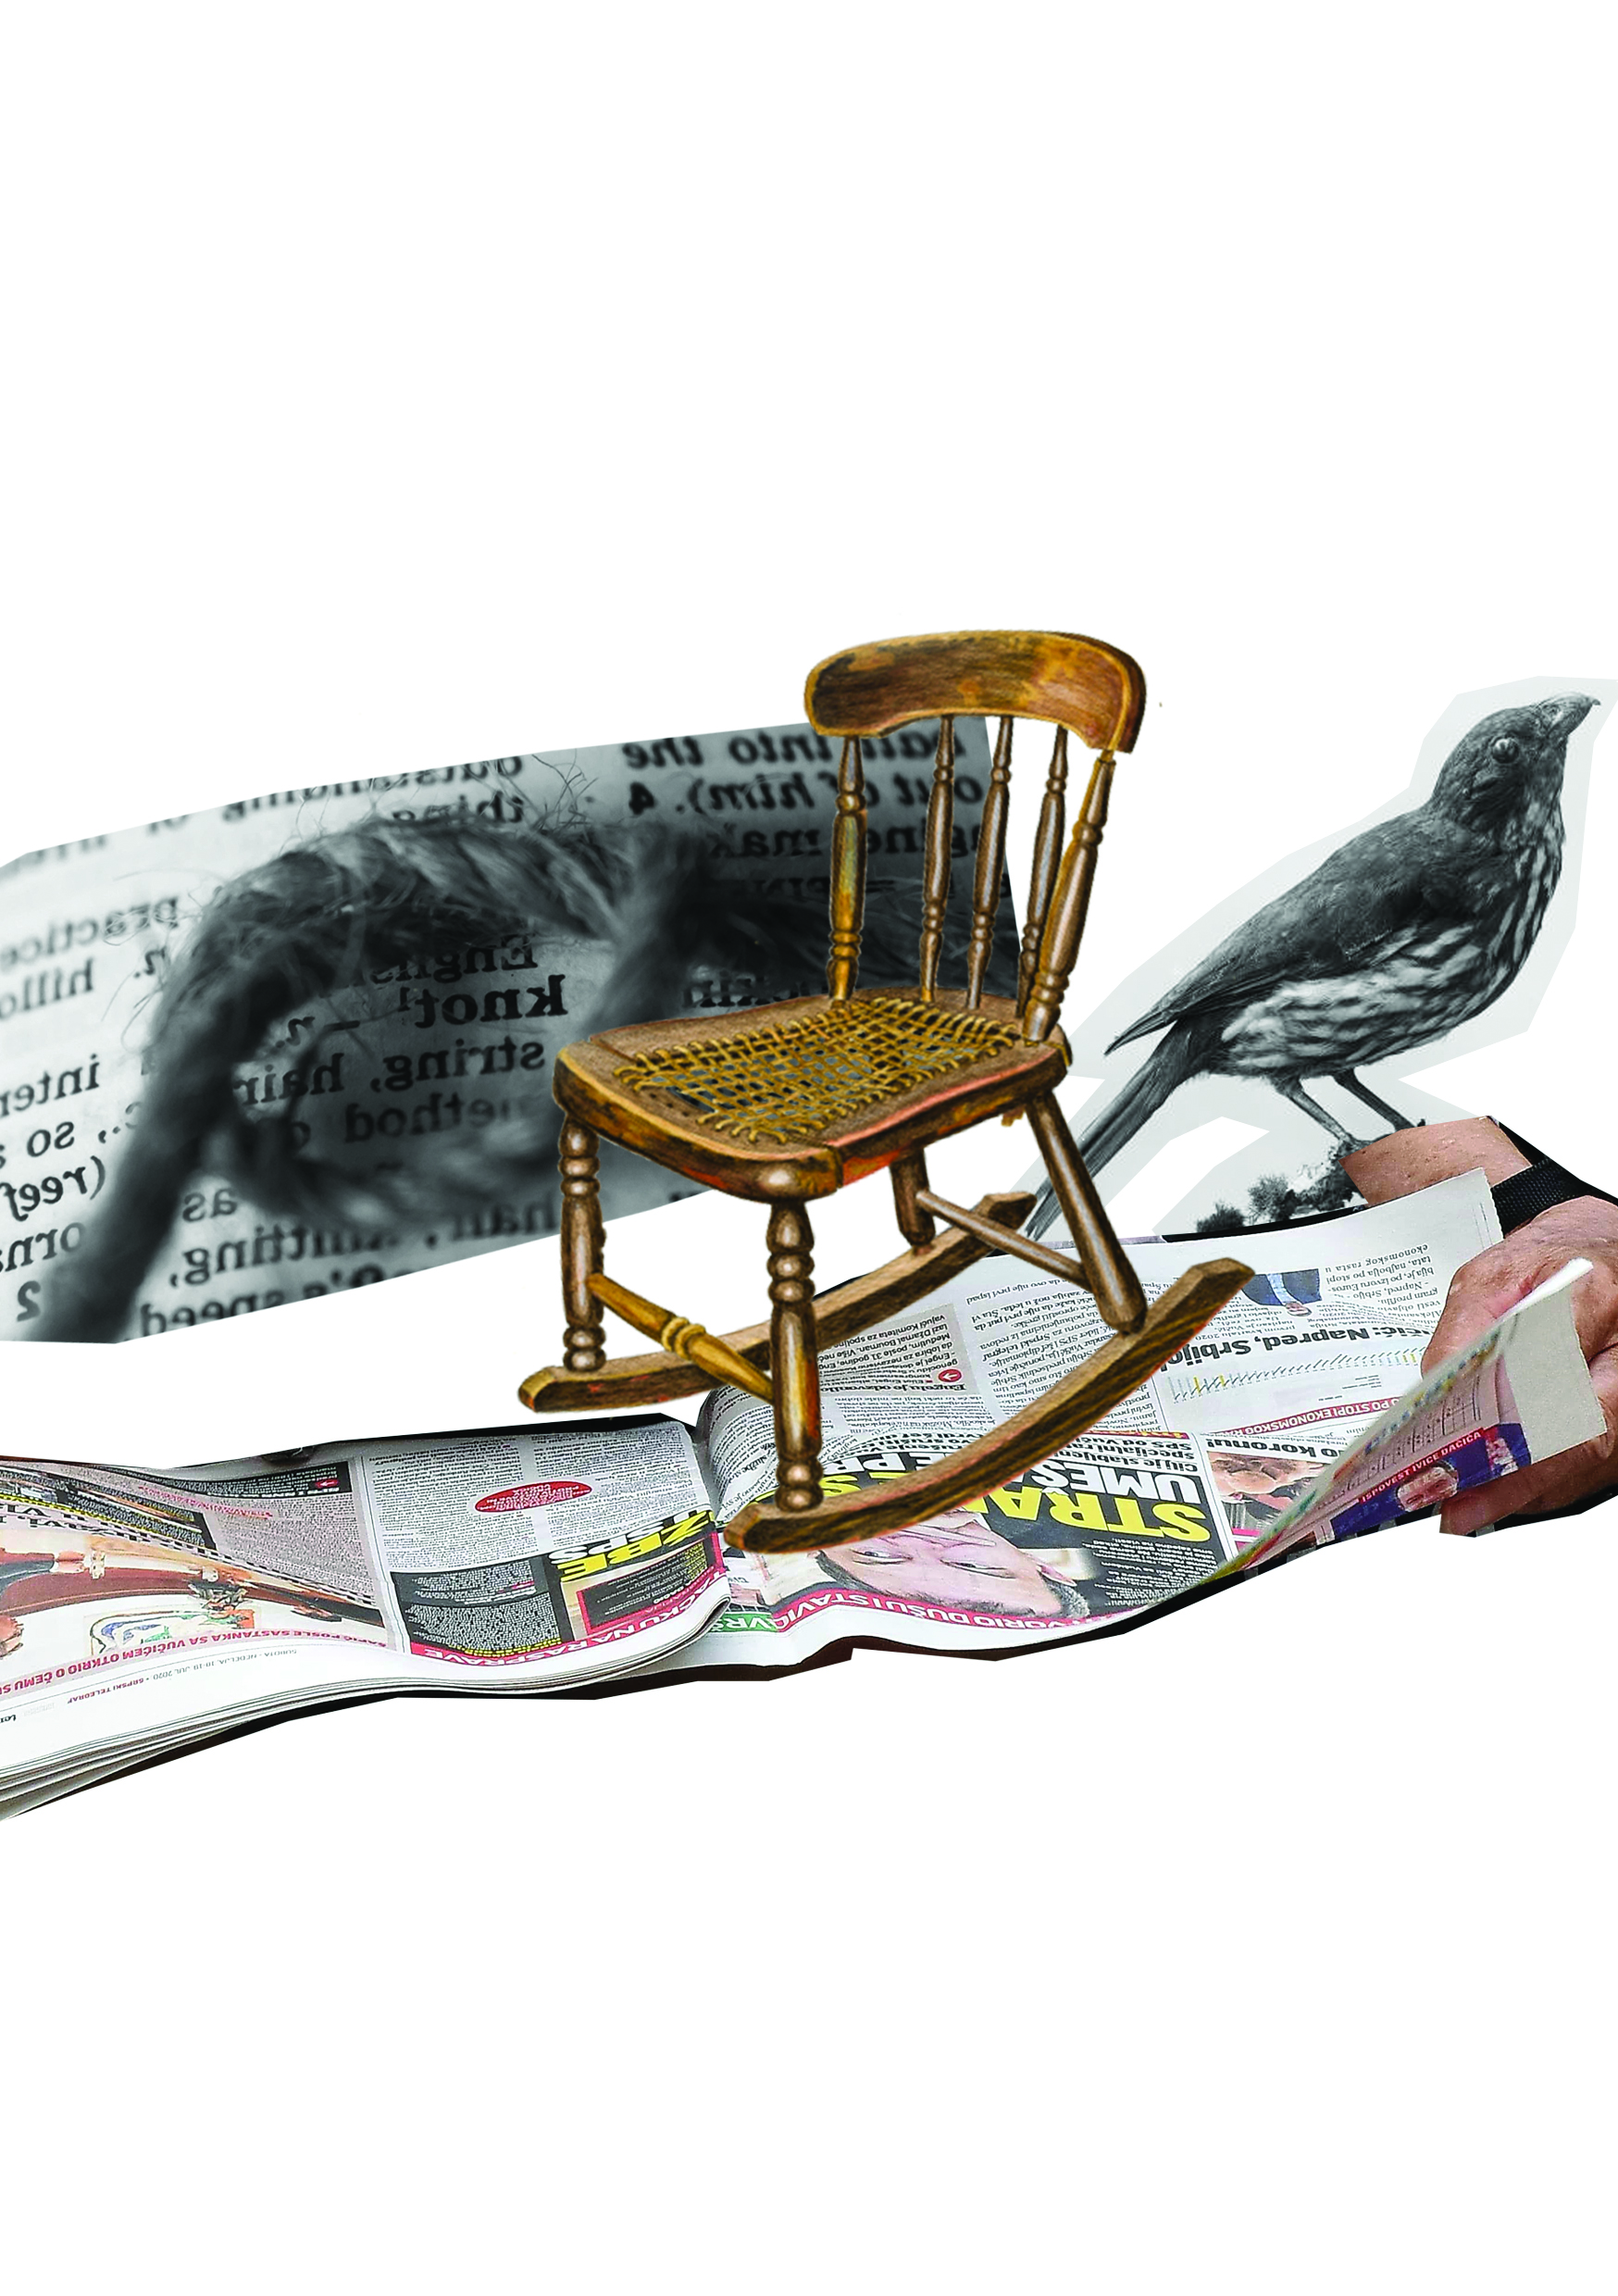
\includegraphics[width=140mm]{../ilustracoes/14_PLEBISCITO.jpg}
\end{figure}
\pagebreak

\chapterspecial{Plebiscito\protect\footnote{plebiscito: consulta sobre
  questão específica, feita diretamente ao povo, geralmente por meio de
  votação do tipo sim ou não.}}{}{Artur de Azevedo}

\noindent{}A cena passa-se em 1890.

A família está toda reunida na sala de jantar.

O senhor Rodrigues palita os dentes, repimpado\footnote{repimpado: bem
  sentado, refestelado.} numa cadeira de balanço. Acabou de comer como
um abade.

Dona Bernardina, sua esposa, está muito entretida a limpar a gaiola de
um canário belga.

Os pequenos são dois, um menino e uma menina. Ela distrai-se a olhar
para o canário. Ele, encostado à mesa, os pés cruzados, lê com muita
atenção uma das nossas folhas diárias.

Silêncio.

De repente, o menino levanta a cabeça e pergunta:

--- Papai, que é plebiscito?

O senhor Rodrigues fecha os olhos imediatamente para fingir que dorme.

O pequeno insiste:

--- Papai?

Pausa:

--- Papai?

Dona Bernardina intervém:

--- Ó seu Rodrigues, Manduca está lhe chamando. Não durma depois do
jantar que lhe faz mal.

O senhor Rodrigues não tem remédio senão abrir os olhos.

--- Que é? Que desejam vocês?

--- Eu queria que papai me dissesse o que é plebiscito.

--- Ora essa, rapaz! Então tu vais fazer doze anos e não sabes ainda o
que é plebiscito?

--- Se soubesse não perguntava.

O Senhor Rodrigues volta-se para dona Bernardina, que continua muito
ocupada com a gaiola:

--- Ó senhora, o pequeno não sabe o que é plebiscito!

--- Não admira que ele não saiba, porque eu também não sei.

--- Que me diz?! Pois a senhora não sabe o que é plebiscito?

--- Nem eu, nem você; aqui em casa ninguém sabe o que é plebiscito.

--- Ninguém, alto lá! Creio que tenho dado provas de não ser nenhum
ignorante!

--- A sua cara não me engana. Você é muito prosa. Vamos: se sabe, diga o
que é plebiscito! Então? A gente está esperando! Diga!\ldots{}

--- A senhora o que quer é enfezar-me!

--- Mas, homem de Deus, para que você não há de confessar que não sabe?
Não é nenhuma vergonha ignorar qualquer palavra. Já outro dia foi a
mesma coisa quando Manduca lhe perguntou o que era proletário. Você
falou, e o menino ficou sem saber!

--- Proletário, acudiu o senhor Rodrigues, é o cidadão pobre que vive do
trabalho mal remunerado.

--- Sim, agora sabe porque foi ao dicionário; mas dou-lhe um doce, se me
disser o que é plebiscito sem se arredar dessa cadeira!

--- Que gostinho tem a senhora em tornar-me ridículo na presença destas
crianças!

--- Oh! ridículo é você mesmo quem se faz. Seria tão simples dizer: ---
Não sei, Manduca, não sei o que é plebiscito; vai buscar o dicionário,
meu filho.

O senhor Rodrigues ergue-se de um ímpeto e brada:

--- Mas se eu sei!

--- Pois se sabe, diga!

--- Não digo para me não humilhar diante de meus filhos! Não dou o braço
a torcer! Quero conservar a força moral que devo ter nesta casa! Vá para
o diabo!

E o senhor Rodrigues, exasperadíssimo, nervoso, deixa a sala de jantar e
vai para o seu quarto, batendo violentamente a porta.

No quarto havia o que ele mais precisava naquela ocasião: algumas gotas
de água de flor de laranja e um dicionário\ldots{}

A menina toma a palavra:

--- Coitado de papai! Zangou-se logo depois do jantar! Dizem que é tão
perigoso!

--- Não fosse tolo, observa dona Bernardina, e confessasse francamente
que não sabia o que é plebiscito!

--- Pois sim, acode Manduca, muito pesaroso por ter sido o causador
involuntário de toda aquela discussão; pois sim, mamãe; chame papai e
façam as pazes.

--- Sim! sim! façam as pazes! diz a menina em tom meigo e suplicante.
Que tolice! duas pessoas que se estimam tanto zangarem-se por causa do
plebiscito!

Dona Bernardina dá um beijo na filha, e vai bater à porta do quarto:

---Seu Rodrigues, venha sentar-se; não vale a pena zangar-se por tão
pouco.

O negociante esperava a deixa. A porta abre-se imediatamente. Ele entra,
atravessa a casa, e vai sentar-se na cadeira de balanço.

--- É boa! brada o senhor Rodrigues depois de largo silêncio; é muito
boa! Eu! eu ignorar a significação da palavra plebiscito! Eu!\ldots{}

A mulher e os filhos aproximam-se dele.

O homem continua num tom profundamente dogmático:

--- Plebiscito.

E olha para todos os lados a ver se há por ali mais alguém que possa
aproveitar a lição.

--- Plebiscito é uma lei decretada pelo povo romano, estabelecido em
comícios.

--- Ah! suspiram todos, aliviados.

--- Uma lei romana, percebem? E querem introduzi-la no Brasil! É mais um
estrangeirismo!\ldots{}

\pagebreak
\thispagestyle{empty}
\begin{figure}
\vspace*{-.5cm}
\hspace*{-2.3cm}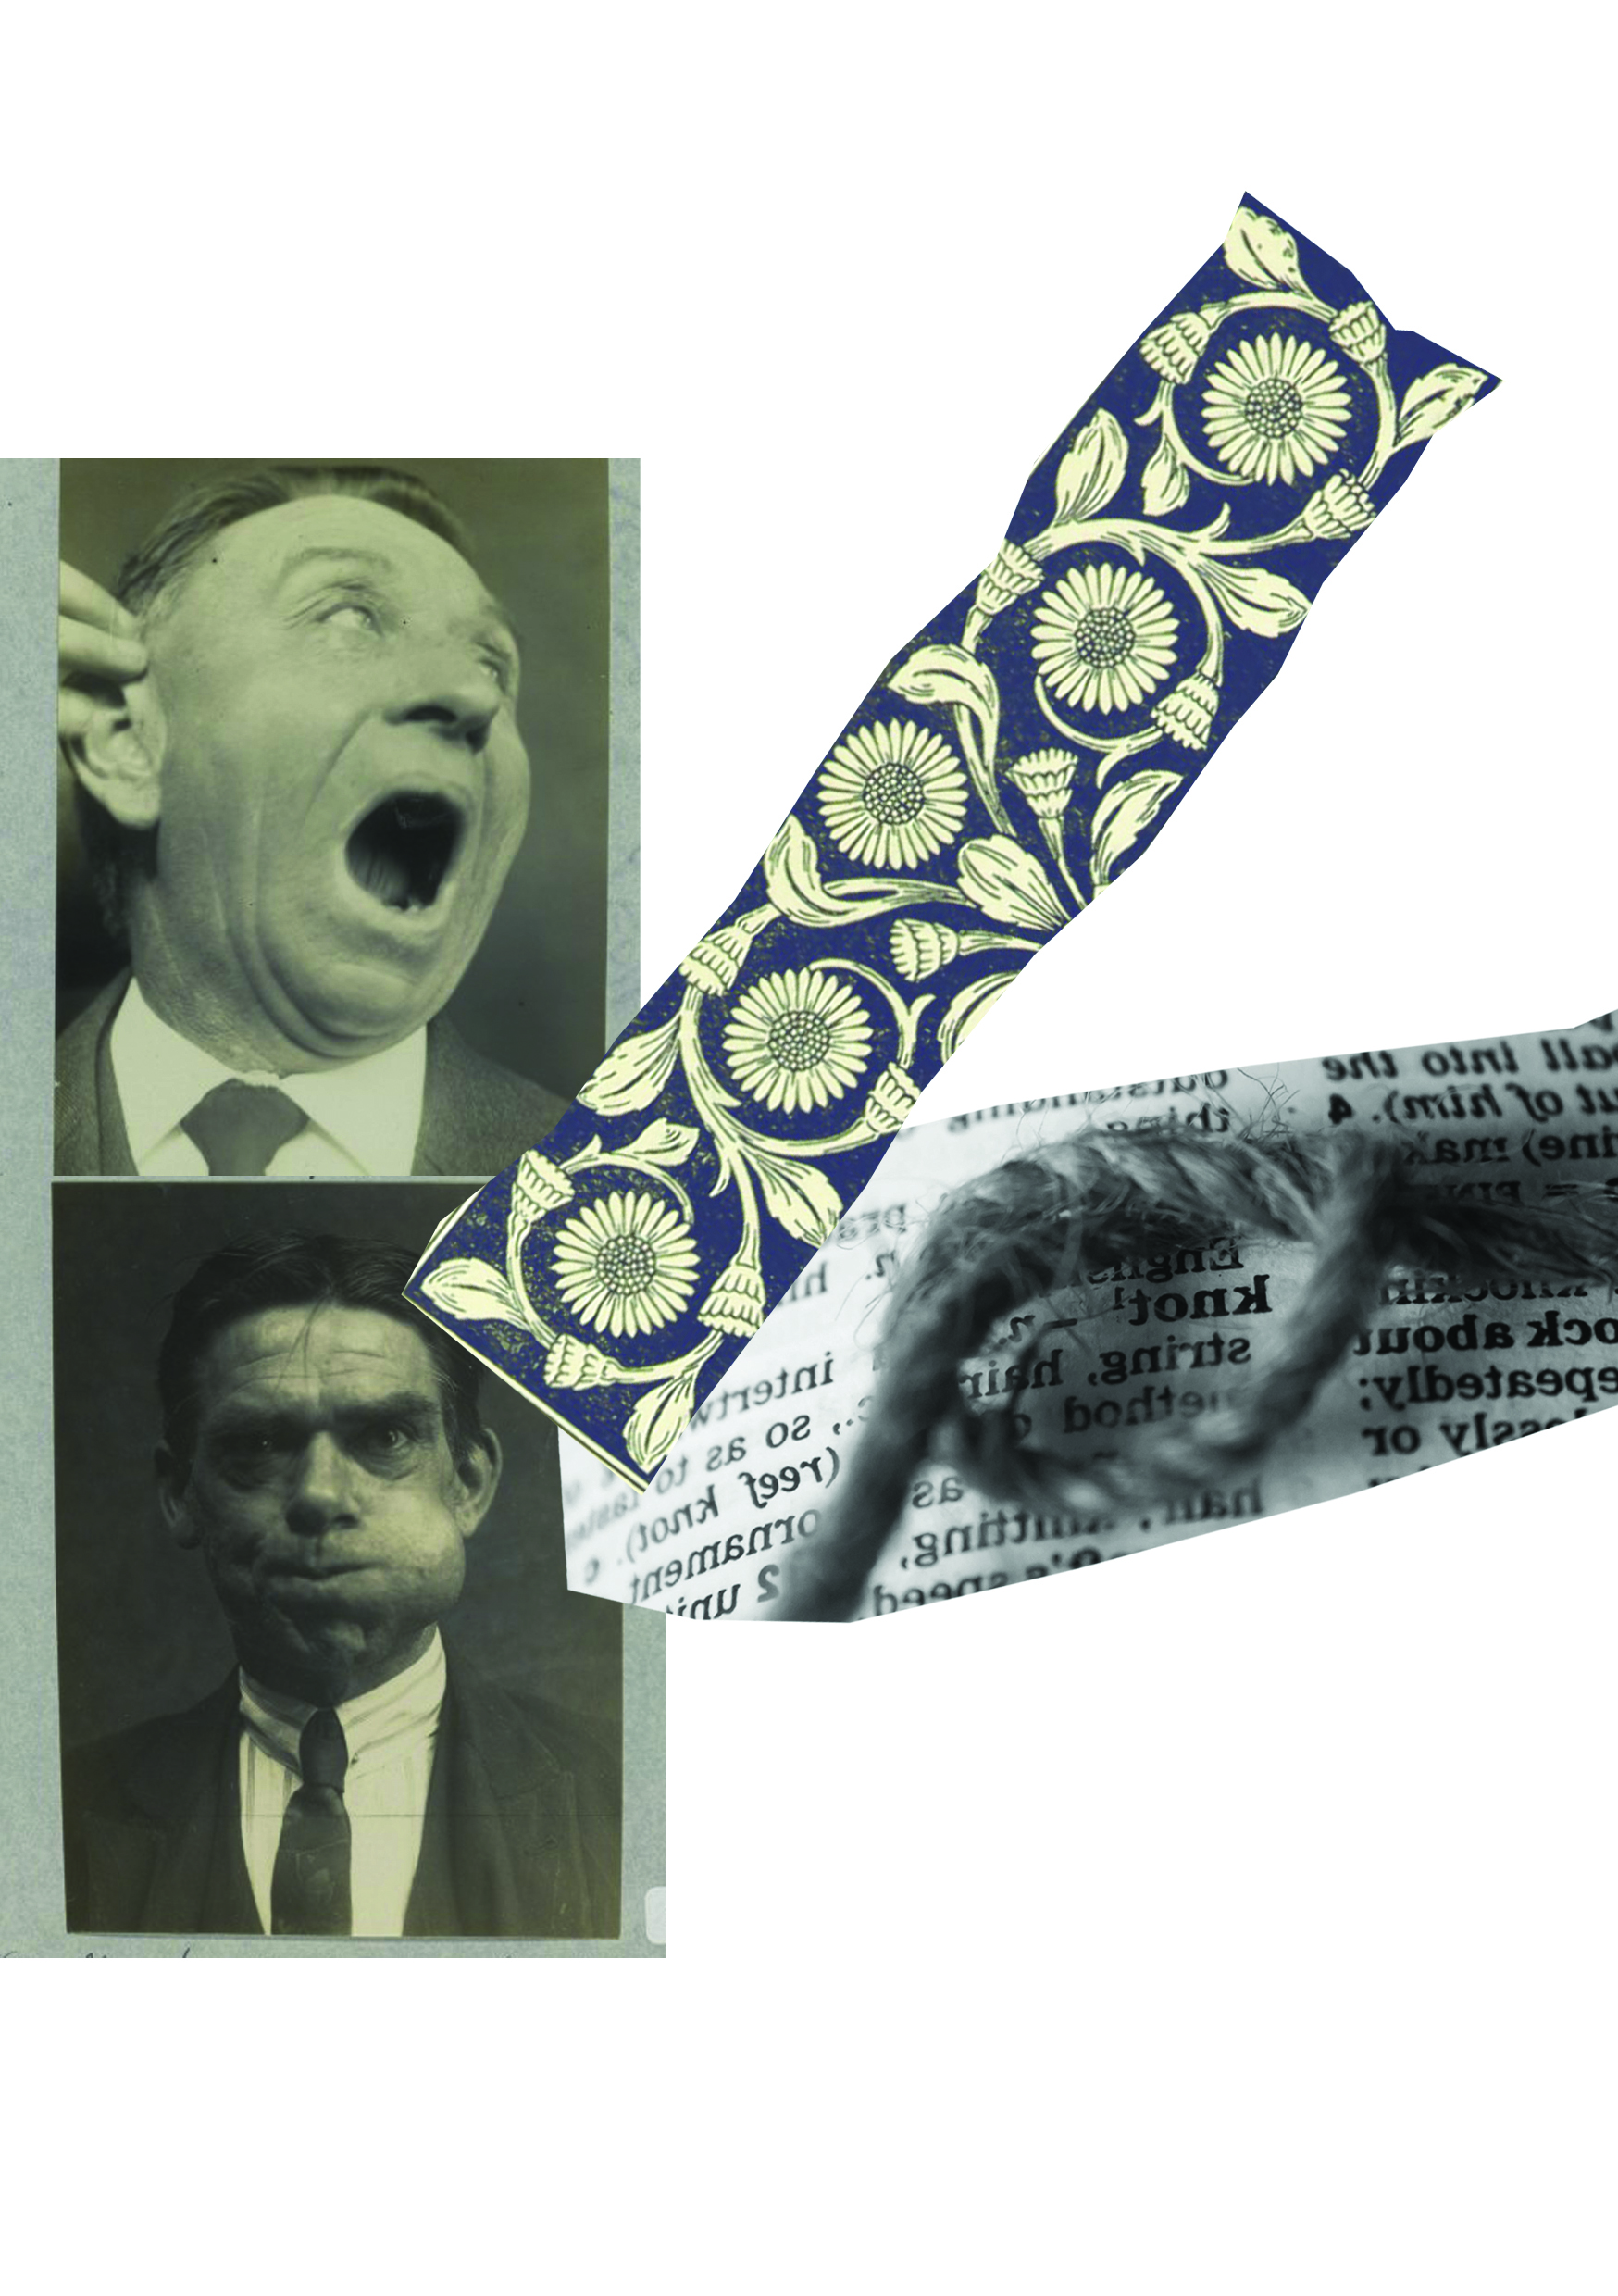
\includegraphics[width=140mm]{../ilustracoes/15_ASNEIRAS.jpg}
\end{figure}
\pagebreak

\chapterspecial{As asneiras do Guedes}{}{Artur Azevedo}

\noindent{}Não é precisamente um conto o que hoje vou escrever.

Voltou do seu passeio a São Paulo o Guedes --- o Guedes sabem? --- o
maior asneirão que o sol cobre, aquele mesmo que respondeu aqui há
tempos quando numa roda lhe perguntaram se tinha filhos:

--- Tenho uma filha já adúltera.

--- Adúltera?!

--- Sim, senhor, adúltera; vai fazer dezessete anos.

--- Adulta quer o senhor dizer\ldots{}

--- Ou isso. É uma boa menina; só tem um defeito: é muito luxuriosa.

--- Luxuriosa?!

--- Sim, senhor, luxuriosa: gosta muito de luxar.

--- Ah!

--- Mas lá está minha mulher para lhe dar bons conselhos\ldots{} sim, porque
minha mulher é muito sensual.

--- Sensual?!

--- Sim, senhor, sensual: tem muito bom senso.

Pois é como lhes digo: tive o prazer de encontrar ontem esse precioso
Guedes, cujas asneiras, colecionadas, dariam um volume de trezentas
páginas, ou mais.

Eu estava num armarinho da rua do Ouvidor, onde entrava para
cumprimentar a minha espirituosa amiga D. Henriqueta, que andava, como
sempre, fazendo compras, enchendo-se de caixinhas e pequeninos
embrulhos, adquiridos aqui e ali:

O Guedes, mal que me viu, correu a dar-me um abraço, dizendo:

--- Li no \emph{O País} a notícia do seu aniversário\ldots{}

E recuando dois passos, tomou uma atitude solene, deixou cair as
pálpebras, e acrescentou:

--- Faço votos para que você tenha um futuro tão brilhante como o que
passou.

Agradeci comovido essa manifestação de apreço envolvida num
disparate,\footnote{disparate: despropósito, tolice.} e apresentei o
Guedes à minha espirituosa amiga D. Henriqueta, que mordia os lábios
para não rir.

--- Apresento-lhe, minha senhora, o mais extraordinário reformador da
língua portuguesa: o Guedes, o grande Guedes, que acaba de chegar de São
Paulo, onde esteve a passeio.

--- Era tempo de fazer uma viagem! --- explicou ele. --- Foi a primeira
vez que saí do Rio de Janeiro.

--- Eu também não saí ainda desta cidade senão para ir uma vez a
Petrópolis e duas a Niterói --- disse D. Henriqueta.

--- Vejo então que a senhora é cortesã\ldots{} --- acudiu o Guedes curvando
os lábios no mais amável dos seus sorrisos.

--- Cortesã?!

--- Cortesã, sim\ldots{} filha da Corte\ldots{}

--- Oh! Guedes! --- observei baixinho. --- Pois você não vê que está
dizendo uma inconveniência?

--- Tem razão\ldots{} Atualmente não se deve falar em Corte\ldots{}

E emendou:

--- Vejo então que a senhora é capitalista federalista.

D. Henriqueta desta vez riu-se a perder. É provável que ao leitor não
aconteça o mesmo. Paciência.

--- Ó Guedes! Vamos lá! Diga-me! Que impressões trouxe de São Paulo?

--- Muito boas! Aquilo é uma grande terra!

--- Dizem que há lá muita sociabilidade.

--- Como?

--- Muita convivência\ldots{}

--- Isso há\ldots{} As famílias visitam-se\ldots{} Os moços coabitam com as moças.

--- Ora essa!

--- Que entende você por ``coabitar''?

--- É\ldots{} é\ldots{}

--- É uma indecência\ldots{} uma inconveniência\ldots{} uma coisa que não se
diz!\ldots{}

O Guedes inflamou-se:

--- Está você muito enganado\ldots{} ``Coabitar'' é\ldots{}

E voltando-se para um dos caixeiros do armarinho:

--- O senhor tem aí um dicionário que me empreste?

--- Pois não?

E daí a dois minutos o Guedes tinha nas mãos os dois volumes do
\emph{Aulete}.

--- Muito bem! --- disse eu. --- Procure ``coabitar''.

Depois de folhear em vão o dicionário durante um ror de tempo, o teimoso
exclamou:

--- Não dá! Não dá! Vejam\ldots{}

--- Perdão: você está procurando com \emph{u}: deve ser com \emph{o}!

--- Tem razão, tem razão\ldots{} Onde estava eu com a cabeça?

E o Guedes pôs-se de novo a folhear o \emph{Aulete}.

--- Não dá! Também não dá com \emph{o}! Veja: de coa para coação! Não dá
com \emph{u} nem com \emph{o}!

Valha-o Deus, Guedes, valha-o Deus! Você está procurando sem \emph{h}?
Dê cá o dicionário!

E com um sorriso de triunfo mostrei ao Guedes a significação da palavra.

--- Olhe, leia: ``Coabitar, habitar, viver conjuntamente''.

--- Mas isso\ldots{}

--- Agora veja o que o \emph{Aulete} acrescenta entre parênteses:

``Diz-se particularmente de duas pessoas de diferente sexo.''

--- Perdão! --- bradou o Guedes furioso. --- Perdão! Eu não disse
particularmente, mas alto e bom som, e só não me ouviu quem não me quis
ouvir!

E batendo com a mão espalmada sobre o balcão:

--- Eu não sou homem que diga as coisas particularmente!

\part{Entre animais}

\pagebreak
\thispagestyle{empty}
\begin{figure}
\vspace*{-.5cm}
\hspace*{-2.3cm}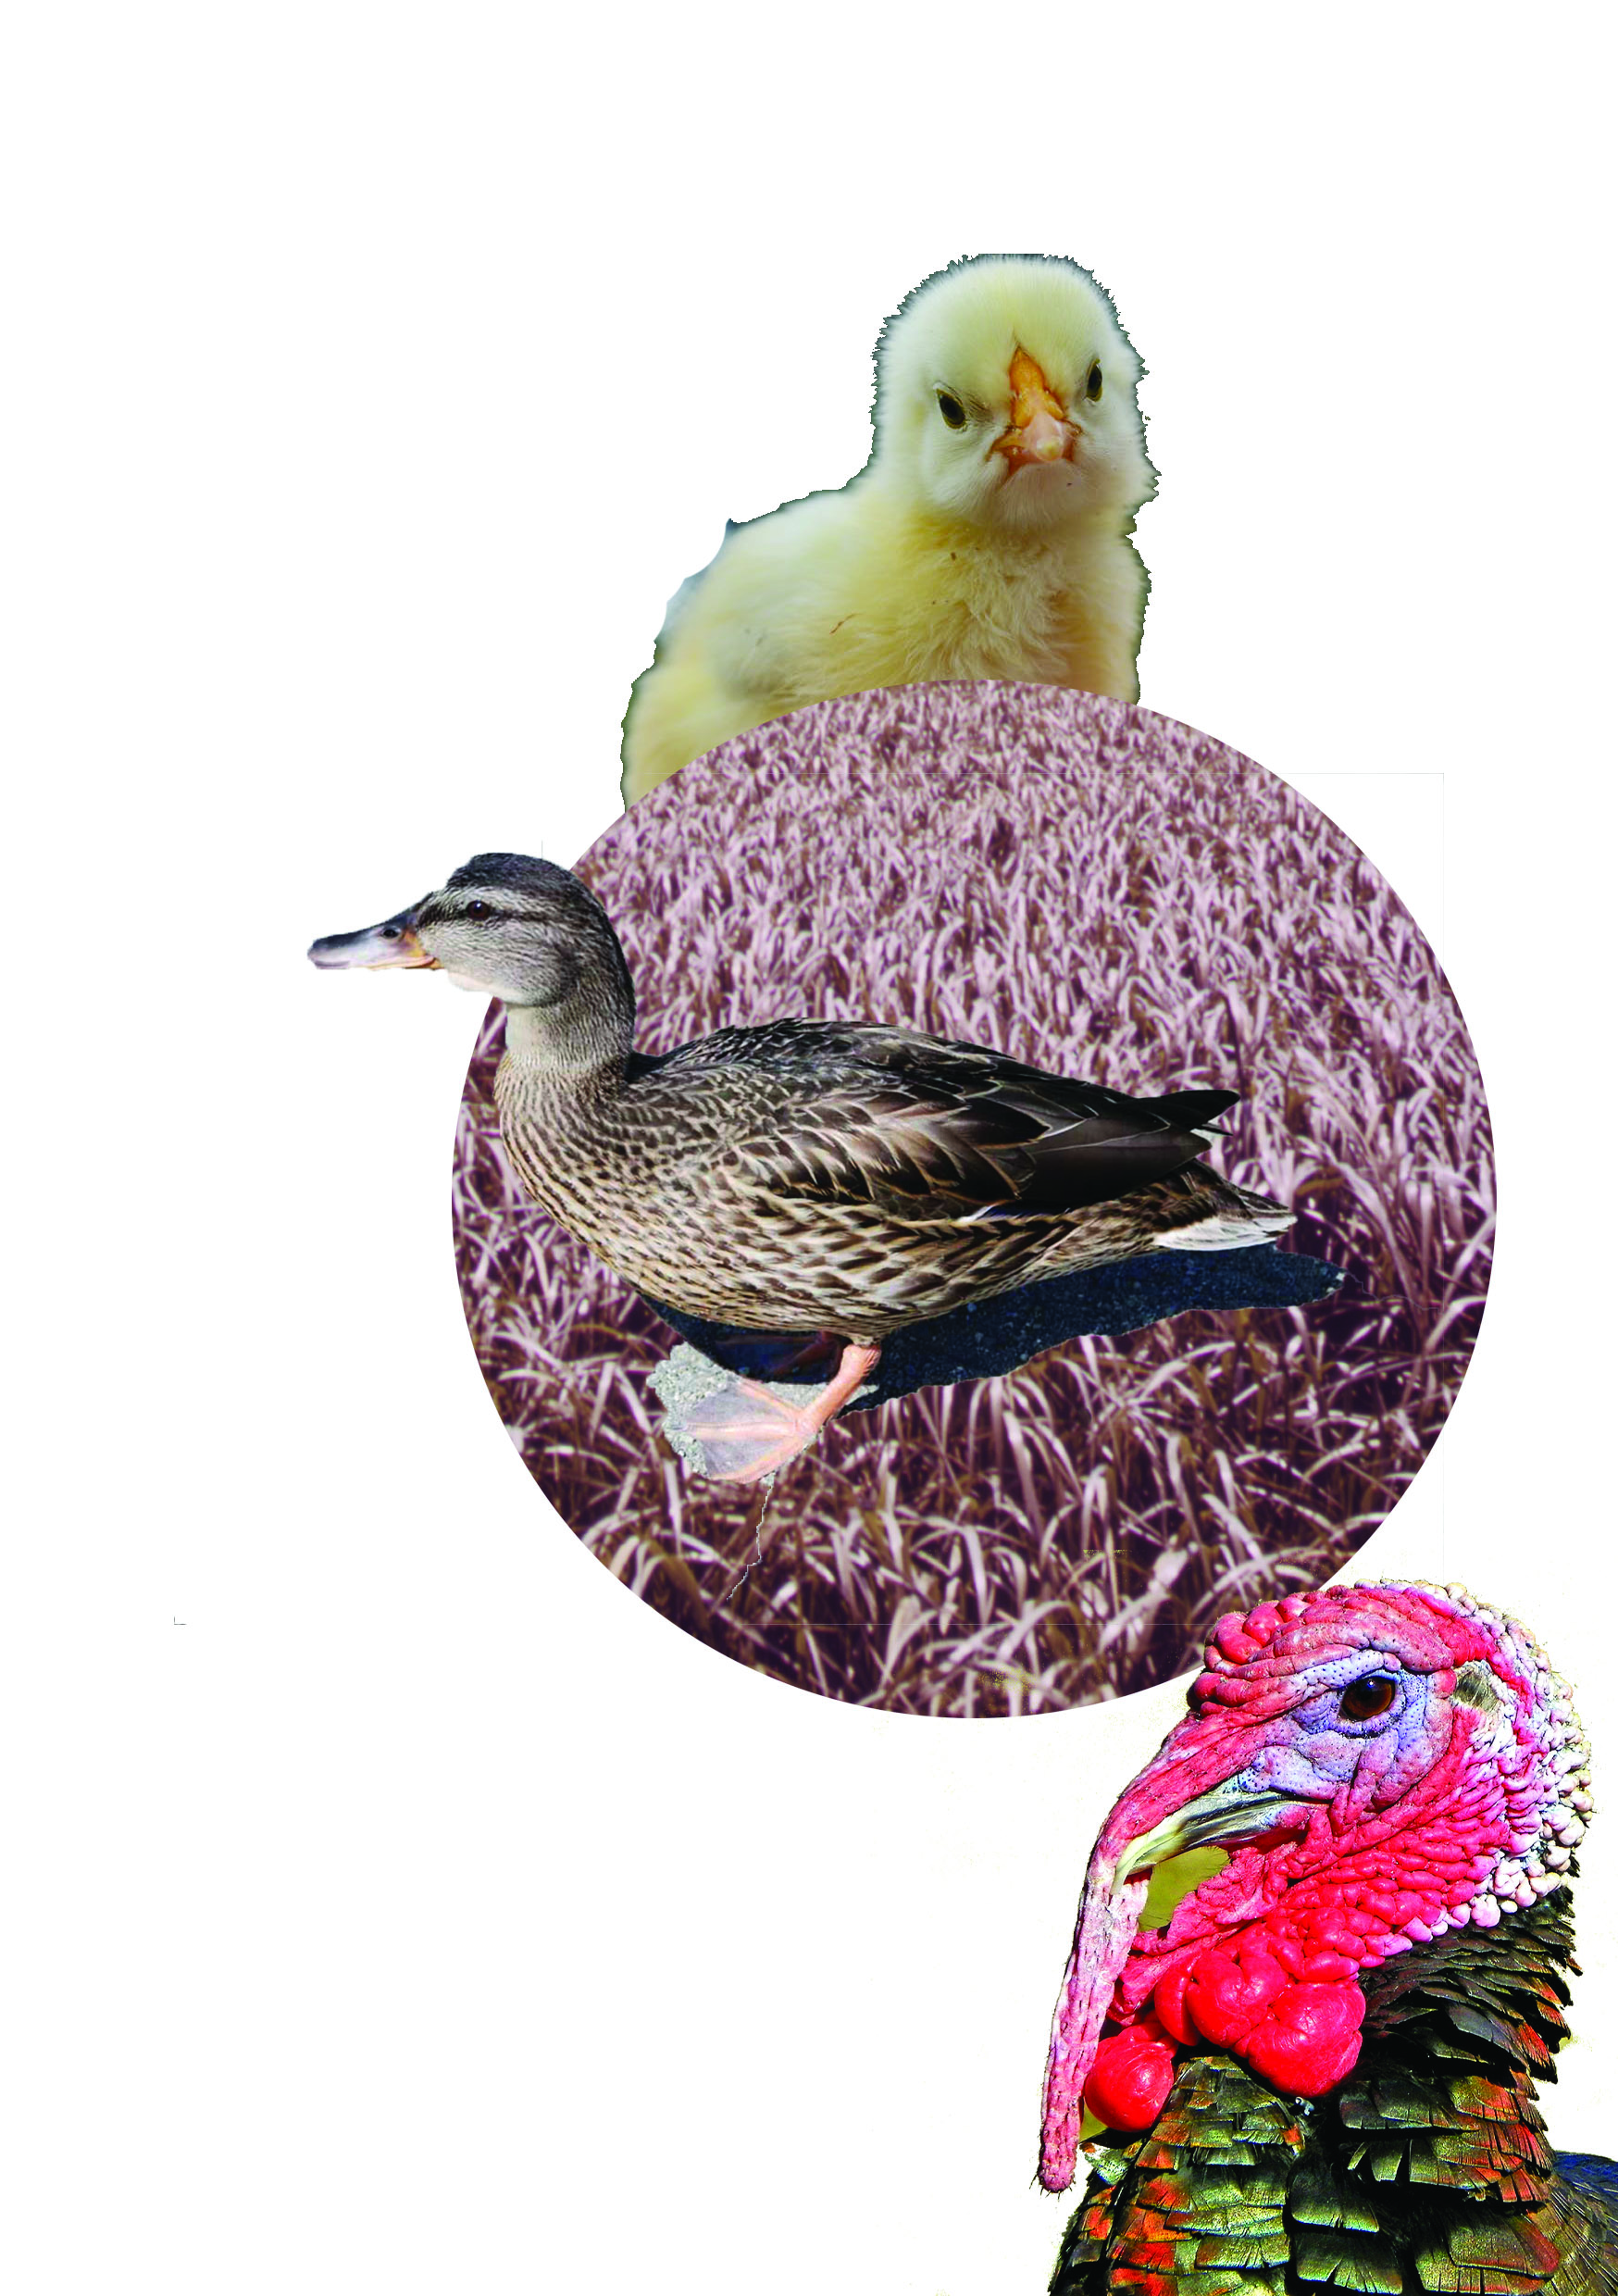
\includegraphics[width=140mm]{../ilustracoes/16_TRAGEDIA.jpg}
\end{figure}
\pagebreak

\chapterspecial{Tragédia dum capão de pintos}{}{Monteiro Lobato}

\noindent{}Nasceram na mesma semana um pinto, um peruzinho e um marreco. Até aqui,
nada. Todos os dias vêm ao mundo marrecos, perus e pintos sem que isso
ponha comichões na pena dos novelistas. O estranho do caso foi que
nasceram irmãos, contra todos os preceitos biológicos.

--- ??

Explica-se. Tio Pio, preto cambaio que tomava conta do terreiro, tivera
a ideia de reunir sob certa galinha, em choco sobre apenas cinco ovos,
mais três de perua e dois de marreca salvos de ninhadas infelizes,
conseguindo assim dar vida àquela estranha irmandade de nova espécie.

Dos nove ovos só vingaram três, e lá estavam os produtos já crescidotes
sob a guarda solícita do Peva-de-raça, capão de pintos posto a pajeá-los
para que dona galinha não perdesse tempo com tão pífia\footnote{pífio:
  de pouco valor.} ninhada.

Triste sorte na fazenda a dos galos cotós de pernas! Tio Pio os punha de
parte para capões de pintos, transformando os belicosos ``clarins da
aurora'' em tristes eunucos,\footnote{eunuco: no Oriente, homem castrado
  que tinha a função de guardar as mulheres do harém.} bichos metade
galo, metade galinha, senhores de crista, espora e cauda flamante não
mais destinadas a seduzir frangas, senão a divertir pintinhos.

Peva-de-raça tinha este nome pelas razões que o nome indica. Mas vá
lição para os leitores da cidade, gente que de galos e galinhas só
conhece os da torre das igrejas e as que aparecem ao jantar em molho
pardo. \emph{Peva}: perna curta; \emph{de raça}: raça estrangeira.

--- A mó que Plimu --- explicava Pio aos interpelantes.

Excelente sujeito o Peva! Tomara os órfãos no primeiro dia sem nenhuma
relutância e dera com eles criados à custa de infinitos de pachorra.

Muitos dissabores sofreu. O marrequinho, sobretudo, causou-lhe sérios
aborrecimentos.

Havia na fazenda um tanque bordado de taboas esbeltas, rico de traíras e
sapinhos de cauda. Esse tanque era a mania do lindo pompom de arminho
amarelo. Quantas vezes não ficou o Peva à beira d'água seguindo de olhos
aflitos as evoluções do mimoso palmípede, que nela penetrava e nadava, e
mergulhava com louca afoiteza, inconcebível para o velho capão!

Já os outros não o afligiam tanto. Divertiam-no até. O capão gostava de
ver o peruzinho em caça às moscas. Magricela e tonto, como sabia marcar
a presa, achegar-se com extrema lentidão e de repente --- \emph{zás!}
--- uma bicada certeira!

O pinto, esse era mestre em travessuras. Subia-lhe às costas,
tenteando-se nas asinhas, e trepava-lhe pelo pescoço até alcançar a
crista, cujas carúnculas bicava.

Era muito cauteloso, o Peva. Se vinha chuva, punha-se logo de agacho
para abrigo dos guris --- de dois apenas, que o terceiro, o marreco,
nenhum caso d'água fazia, antes pelava-se por chuva, só recolhendo ao
sentir-se entanguido.

E era muito metódico, o Peva. Mal a tarde fechava a carranca anunciativa
da noite, lá ia ele de rumo ao terreiro aninhar-se rente ao muro, sempre
no mesmo lugar. Escarrapachava-se ali ao jeito das galinhas e esperava
que os órfãos, depois dumas derradeiras voltas por perto, viessem
chegando e se metessem dentro da plumosa casa viva.

Entrava primeiro o peru, um friorento de marca; depois o pinto; o
marreco por último.

E o Peva cochilava, transfeito em esquisito animal de quatro cabeças: a
sua, grande, cristuda, e mais três cabecinhas curiosas, que abriam
seteiras na plumagem e espiavam o mistério do mundo a envolver-se nas
sombras da noite.

Aquela singularidade deu nome e renome aos três bichinhos. Quantos
pintos, perus e marrecos houvesse na fazenda eram todos conhecidos por
pinto, peru e marreco, genericamente. Só eles se personalizavam. Eram o
Pinto Sura, o Peruzinho do Capão e o Reco-Reco. Seres privilegiados,
libertos da disciplina comum do galinheiro, tornaram-se logo as
criaturinhas mais populares daquele pequeno mundo. Viviam soltos sem lei
nem grei, como boêmios errantes encontradiços por toda parte --- nos
chiqueiros, nos pastos, ao pé das tulhas, à porta das cozinhas, onde
quer que aparecesse fartura de milho, siriris e quireras.

Havia na fazenda outros animais populares. Havia a Ruça, mulinha de
carroça, bastante velha e próxima da aposentadoria. Só trabalhava em
serviços leves de terreiro, puxando a ``carrocinha de dentro''.
Pertencera à tropa, transportara muito café para a cidade, sempre com
carga de oito arrobas, façanha de que, com saudades, se recordava agora.

Entre as vacas era a Princesa a mais popular. Vaca de estimação.
Enriquecera a fazenda de numerosos filhos, entre os quais o possante
Beethoven, agora pastor do rebanho. Dera ainda a Rosita, leiteira de
truz\footnote{de truz: de qualidade.} fiel à estirpe\footnote{estirpe:
  raça, origem.} e certa nas doze garrafas diárias. E quantas outras
crias que já andavam por sua vez de bezerrinho novo, ou na canga, a
puxar carros! Vivia às soltas, livre de cercas, sempre no pasto dos
porcos, ocupando o tempo em mascar babosamente boas palhas de milho.

Quem mais? Sim, o Vinagre --- fiel guardião da ``casa-grande'', veadeiro
de fama outrora, hoje um dorminhoco que o que fazia era cochilar ao sol,
de focinho entre as patas e olhos lacrimejantes. Todo ele era passado.
Durante as sonecas vinham agitá-lo pesadelos, nos quais reviviam as
cenas violentas das caçadas de antanho. E o glorioso veterano acuava a
dormir.

Os homens nunca prestam grande atenção aos animais que os rodeiam.
Brutinhos, dizem, e desprezam-nos. Mas a verdade é que a esses nossos
manos o que os inferioriza é não gozarem o dom da fala, pelo menos de
fala inteligível para nós, visto como pensam e superiormente raciocinam,
possuindo sobre os homens e as coisas ideias terrivelmente lógicas.

Ali na fazenda eram todos concordes num ponto: a supremacia de Tio Pio
sobre os demais seres humanos. Era Tio Pio a atenção que nada esquece, a
justiça que dá e pune, o amor que compreende, o deus que cura, a ordem
que tudo simplifica.

Para o trio do Peva era Tio Pio o Recolhe-ovos, o Deita-ninhadas, o
Matapiolho, o Varre-galinheiro, o Pega-frango, o Arruma-ninho, o
Traz-quirera, o Rebenta-cupim, o Espanta-cachorro --- modalidades várias
dum alto espírito de providência.

Para a Princesa era o Traz-milho, o Tira-leite, o Prende-bezerro, o
Esvurma-berne, o Fecha-porteira, o Bota-no-pasto.

Para a mulinha era o Põe-carroça, o Arruma-arreios, o Escova-pelo, o
Daração.

Para o Vinagre era o Lava-cachorro, o Traz-angu, o Atiça-atiça, o
Pregapontapés.

Só ele, entre tantos homens da fazenda, revelava-se, apesar de preto,
claro de intenções e compreensível; só ele não podia desaparecer sem
grave dano geral. Lembravam-se de como todos padeceram certa ocasião em
que Tio Pio caiu de cama. Houve desordem grossa. Pintos morreram de
fome; Vinagre emagreceu; a Princesa viu-se privada de palha; o Peva
dormiu fora do terreiro pela primeira vez. Ao cabo de dez dias, quando o
preto ressurgiu, recém-sarado, foi como se repontasse o sol em seguida a
longo tempo de chuvas. Que alegria!

As demais criaturas humanas afiguravam-se-lhes misteriosas e sobretudo
ilógicas. Impossível ao Vinagre entender o patrão. Já de cara alegre, já
de cara amarrada, recebia-o alternativamente com carinho ou pontapés. E
o velho cachorro filosofava: como é que um mesmo ato meu, sempre gesto
de afago e submissão, ora recebe prêmio, ora castigo? Não entendia\ldots{}

E muito menos o entendiam o Peva, a Princesa e a Ruça. Sua presença no
curral ou no pasto era signo certo de calamidade --- morte, prisão,
tortura. ``Mate aquele boi'', ``Pegue aquele frango'', ``Arreie aquele
cavalo'', ``Cape aquele porco''. Mate, pegue, arreie, cape, venda,
esfole --- não se lhe ouviam outras palavras. E toda gente corria
pressurosa a executar-lhe as ordens, por mais tirânicas que fossem.

Igualmente incompreensíveis eram os filhotes do homem. Que criaturinhas
variáveis, irrequietas, cruéis! Sempre de vara na mão, perseguiam
abelhas e borboletas, esmagavam os sapos, atropelavam as galinhas. Ao
vê-las, Vinagre disfarçadamente saía para longe e o Peva bandeava-se com
seus órfãos para o outro lado dalgum vedo. Só a Princesa nenhum caso
deles fazia, certa do terror que lhes inspiravam os seus longos chifres.

Já a Dona, mulher do Senhor, não infundia medo senão às aves. Terrível
inimiga do galinheiro! Depredava os ovos e condenava à morte justamente
os mais belos frangos e as mais respeitáveis matronas de pena ---
``galinhas velhas'', como dizia a ingrata.

Para os outros animais a Dona significava apenas ignorância. Era a
``Perguntativa'' e a ``Muda-cor''. Hoje de cor-de-rosa, amanhã de azul,
não usava cor fixa. E vivia interrogando:

--- Pio, que burro é esse?

--- Não é burro, sinhá, é a mulinha Ruça.

Perguntava sempre. Que \emph{caroços} eram aqueles na vaca? Que boi
estava \emph{rinchando} no pasto? Que \emph{trepadeira} andavam a tirar
das árvores?

Viera duma cidade grande, havia pouco tempo, cheia de gritinhos e medo
aos bichos. Ignorava tudo, fora pilhar ninhos. \emph{Papa-ovo},
apelidou-a o Peva, como já havia apelidado Tio Pio de \emph{É-hora} e
aos demais camaradas da fazenda de \emph{Sim-Senhores}, porque \emph{Sim
Senhor} era o estribilho com que habitualmente retrucavam a todas as
ordens do Dono.

Por uma tarde igual às outras, recolhia-se Peva ao pouso do costume
seguido dos três órfãos já marmanjões. No céu, a caraça vermelha do sol
escondia-se detrás do morro, e na terra os primeiros grilos ensaiavam as
asas cricrilantes. Rente à porteira a mulinha, solta no pasto minutos
antes, espojava-se regalada.

--- Boa tarde! --- saudou-a o Peva. --- Cansadinha, hein?

A mula interrompeu a cabriola e abanou as orelhas como quem diz: ``É
verdade''. Depois falou:

--- Acho prudente que tome cuidado com seus filhos. A Perguntativa anda
interessada por eles --- e isso é mau sinal. Vi-a em conversa com É-hora
e pilhei este pedacinho: ``O marreco do capão está no ponto''. Não sei o
que quer dizer, mas boa coisa não será.

O Peva enrugou a testa, apreensivo. Jamais a Perguntativa se referia a
alguma ave sem que sobreviesse desgraça. ``Está no ponto'' --- que
quereria dizer aquilo?

A mulinha ignorava-o. Sabia de algumas palavras triviais, conhecia o
\emph{pegue}, o \emph{prenda}, o \emph{mate} --- mas o \emph{está no
ponto} era-lhe coisa nova.

--- Quem há de saber disto é o Vinagre. Mora na casa-grande e entende a
língua dos homens melhor do que nenhum de nós. Consulte-o, e não deixe
também de consultar a Princesa, cuja experiência da vida é grande.

Peva se foi à Princesa, que encontrou mascando as palhas do costume.

--- \emph{Está no ponto} --- poderá dizer-me, senhora Princesa, que
coisa significa na língua dos homens?

A vaca interrompeu a mascação e disse:

--- Já ouvi essa palavra aplicada ao meu filho segundo, o Barroso. Tinha
ele dois anos e meio. O Dono passava em companhia de um Sim-Senhor.
Avistou de longe o meu Barroso no pasto e ordenou: ``Aquele boizinho
está no ponto. Carro com ele!''. No dia seguinte laçaram-no, meteram-no
na canga e o pobre do meu garrote muito que padeceu a puxar um carro
pesadíssimo. Deste incidente concluo que \emph{estar no ponto} quer
dizer \emph{carro}.

Peva, um tanto curto de ideias, tremeu ante aquela revelação. Horror,
meterem no carro ao seu querido marrequinho! Em seguida duvidou. Andar
no carro era coisa que só vira fazer aos bois. Não podia ser. A vaca
errara evidentemente.

``Resta-me consultar o Vinagre'', refletiu, e todo pepé, com ruguinhas
de apreensão na crista, foi ter com o velho cachorro.

Vinagre não resolveu o enigma, embora respondesse como o mais sábio dos
oráculos.

--- Pode ser muita coisa. A linguagem dos homens varia, ora quer dizer
isto, ora aquilo. Mas que não é coisa boa, isso eu asseguro.

Nesse dia o capão, seguido dos órfãos, recolheu-se ao pouso habitual sem
a despreocupação de outrora. Custou-lhe conciliar o sono. Não lhe saíam
da cabeça as palavras misteriosas e de sentido inapreensível. Por fim
dormiu e sonhou. Sonhou que ao lado do Barroso jungiam ao carro o pobre
marrequinho.

O sonho virou pesadelo e Peva sofreu horrores ante o quadro do filho
adotivo a debater-se sob a monstruosa canga\ldots{}

No dia seguinte, no momento da ração de milho, Tio Pio inesperadamente
agarrou o marrequinho pelas pernas e lá se foi com ele para a Cozinha.

Aflitíssimo, tomado de imenso desespero, Peva inda alimentou esperanças
de vê-lo. Mas a noite chegou e com ela a primeira desilusão de sua vida.
Nada do marreco. Pela manhã, nada. Meio-dia, nada.

À hora do jantar encontrou Vinagre roendo uns ossos no terreiro.

--- Que é isso, amigo?

--- Ossos de marreco.

--- De marreco! --- exclamou Peva, surpreso.

--- Sim. Que admiras? Que os marrecos tenham ossos? Têm-nos, e
excelentes\ldots{}

Peva estarreceu. Compreendia afinal o tremendo sentido das palavras
misteriosas. \emph{Está no ponto} significava condenação à morte.
Horror!\ldots{}

Guardou consigo, entretanto, aquela mágoa. Nada disse ao peruzinho nem
ao frango, prevendo para os dois sorte idêntica.

--- Bem triste a vida sob o domínio cruel do homem! Nada de bom vem
deles\ldots{} --- filosofou.

Nessa mesma tarde Peva cruzou-se com a Princesa e disse-lhe:

--- Erraste, Princesa. \emph{Está no ponto} quer dizer \emph{morte}.

A vaca parou a mastigação da palha e sorriu da ingenuidade do Peva. Ela
tinha tanta certeza de que queria dizer \emph{carro}\ldots{}

A vida na fazenda rolava na mesmice de sempre. Tudo continuava. A Ruça,
a puxar a carrocinha; a Princesa, a mascar palhas; o Vinagre, a acuar em
sonhos. Só na tribo do Peva a alegria não era a mesma. Saudades do
marreco. Várias vezes o frango indagou do destino de Reco-Reco, forçando
o capão a mentir. ``Anda de viagem, uma longa viagem\ldots{} Um dia volta.''

Mas com que tristeza punha os olhos no tanque ou nas poças de enxurro
que se formavam em dias de aguaceiro, pensando lá consigo: ``Nunca
mais!''\ldots{}

O tempo corre, as estações se sucedem. A primavera anunciou-se nos mil
botões que se arredondavam nas laranjeiras. Os órfãos do capão já eram
mais companheiros de ciscagem do que filhotes pipilantes. Já dispensavam
a sua solícita assistência. O peruzinho, grandalhudo e bem empenado,
fez-se independente. O frango punha crista, com as esporas abotoadinhas.
Mudara de gênio, e se via alguma franga ia arrastar-lhe a asa até que
algum galo de verdade o escorraçasse.

Certa manhã a Perguntativa veio assistir à amilhagem das aves. Fez
várias perguntas e deu várias ordens ao Pio, concluindo, de dedo
apontado para o frango:

--- Está pedindo panela, aquele!

--- Qual, Sinhá? O Sura?

--- Sura quer dizer sem rabo? É. É ele mesmo.

Peva, que tudo ouvira, engasgou-se com o grão de milho que tinha no
bico, perdeu a fome e incontinenti saiu do bando. Embora não
compreendesse o sentido daquelas palavras, previu que ``boa coisa não
seria'', como filosofava o Vinagre.

E acertou. O frango, no dia imediato, desapareceu misteriosamente. Peva
procurou-o por todos os cantos e, desconfiado, foi rondar os fundos da
Cozinha na esperança de ouvi-lo piar lá dentro. Não ouviu pio nenhum ---
mas encontrou penas suspeitas no monte de lixo\ldots{}

Adquirida a certeza do novo desastre, fez-se ainda mais tristonha a vida
do pobre capão. A Cozinha! Era nas goelas daquele horrendo Moloch que
sucessivamente iam desaparecendo os seus queridos órfãos. Engolira o
marreco, engolira o frango\ldots{} Engoliria também o peruzinho, por que não?

Velho e desalentado, com o coração sempre saudoso dos travessos
garotinhos que criara, tornou-se macambúzio. Inda passeava com o peru,
apesar da cada vez maior independência deste. Chegou a notar que era
ele, Peva, quem o acompanhava agora. Notou-o, mas procurou iludir-se e
simulava amadrinhá-lo, como outrora\ldots{}

Pela força do hábito inda dormiam juntos, no antigo pouso ao pé do muro.
Mas logo o peru, que é amigo de poleiro, elegeu um, cômodo, em certa
escada velha, e o capão teve de acompanhá-lo na mudança. E ali passaram
a dormir juntinhos e encorujados no mesmo degrau.

Assim viveram até a chegada do Ano-Bom.

Na véspera a Perguntativa apareceu no momento do dar milho e disse ao
Pio:

--- Olhe, amanhã temos o peru. Não esqueça de comprar pinga.

Desta feita Peva não vacilou quanto ao sentido da expressão. \emph{Está
no ponto} --- \emph{panela} --- \emph{temos o peru} --- deviam ser
frases equivalentes. Estava pois condenado a entrar para a Cozinha o seu
derradeiro filho\ldots{}

Cheio de resignação e com a alma em transes, Peva passou o dia num
canto, jururu, remoendo as doces recordações de outrora. Ao cair da
noite recolheu-se. Empoleirou-se na velha escada e achou muito natural
que o peru não comparecesse.

Dormiu tarde e teve o sono agitado de contínuas estremeções de angústia.

No dia seguinte notou movimento fora do comum na casa-grande. Vinha
gente de longe, mulheres de trole, homens a cavalo. Vinagre, esquecido
da soneca do costume, entrava e saía, abanando a cauda com vivacidade de
cachorro novo.

Num destes vaivéns Peva o deteve.

--- Que há na casa-grande? Tanta gente\ldots{}

--- Há peru --- respondeu o cão. --- Quando há peru, os homens se
assanham, vestem roupas novas, brincam e dançam. Tenho notado que a
presença do peru à mesa provoca nos homens uma espécie de delírio, como
entre as galinhas a queda de içás.

Esta observação do cachorro, embora muito lisonjeira para a raça dos
perus, não consolou nada ao nosso Peva, que se sentia ganho menos de
tristeza que de funda indiferença pela vida. O sucessivo sacrifício dos
filhotes calejara-lhe por partes o coração. No dia do marreco a dor que
sentiu foi verdadeira dor de pai; em seguida, pela morte do frango, a
sua dor foi dor de pai adotivo; agora, ao perder o peru, a dor era calma
e resignada. Dor de filósofo. Compreendia, afinal, que a vida foi e é
assim, e não melhora\ldots{}

Os capões inspiram desprezo aos galos e talvez piedade irônica às
senhoras galinhas. Por isso Peva, em sua triste solidão, deambulava pelo
terreiro como criatura sem lugar na vida. As lindas frangas, as viçosas
poedeiras, e até as velhas galinhas aposentadas, tinham pela sua honesta
companhia um profundo desdém. E como nem os frangotes o procuravam, o
isolamento do triste eunuco era completo.

Esse errar à toa fê-lo notado de Tio Pio, que se lembrou de pô-lo a
criar nova ninhada.

--- Anda vadiando aqui, este diabo\ldots{} Espera que te arrumo.

Agarrou-o, levou-o ao galinheiro, esfregou-lhe urtiga no abdome e
deitou-o sobre uma ninhada de dez pintos nascidos na véspera.

Não ofereceu Peva a menor resistência. Deixou fazer. Agachou-se como
dantes e cobriu lindamente os gentis recém-nascidos.

Altas horas, porém, ergueu-se e tomou rumo do poleiro, abandonando aos
frios da noite a roda de vidinhas pipilantes. Não mais queria exercer a
profissão de mãe. Para quê?

--- Se têm de morrer na Cozinha, morram agora enquanto ainda não lhes
tenho amor.

Os pintos amanheceram mortos, entanguidos de frio.

Quando Tio Pio tomou conhecimento do desastre, ficou furioso.

--- Cachorro! Você fez mas paga!

Houve um corre-corre. A galinhada assustadiça debandou; os marrecos
meteram-se no tanque.

Cotó de pernas, frouxo de asas, Peva pouco resistiu à perseguição do
negro.

Rendeu-se e, seguro pelas patas, de cabeça para baixo: com as ideias
perturbadas pela congestão do cérebro, por sua vez transpôs a soleira da
Cozinha, insaciável sorvedouro de vidas, odioso túmulo de Reco-Reco, do
Sura, do Peru e agora do venerável tutor da estranha irmandade\ldots{}

Quem na manhã do dia seguinte passasse pelo fundo da horta veria no
monte de lixo um punhado de penas escaldadas, escorridas, sem cor, sujas
de cinza. E veria duas pernas rugosas de longas esporas recurvas. E
veria ainda uma dolorosa cabeça de crista violácea, com os olhos
semiabertos, em cujas pupilas de vidro várias formiguinhas se miravam.

Horríveis, aqueles despojos?

Um urubu pousado ali perto não pensava assim\ldots{}

\pagebreak
\thispagestyle{empty}
\begin{figure}
\vspace*{-.5cm}
\hspace*{-2.3cm}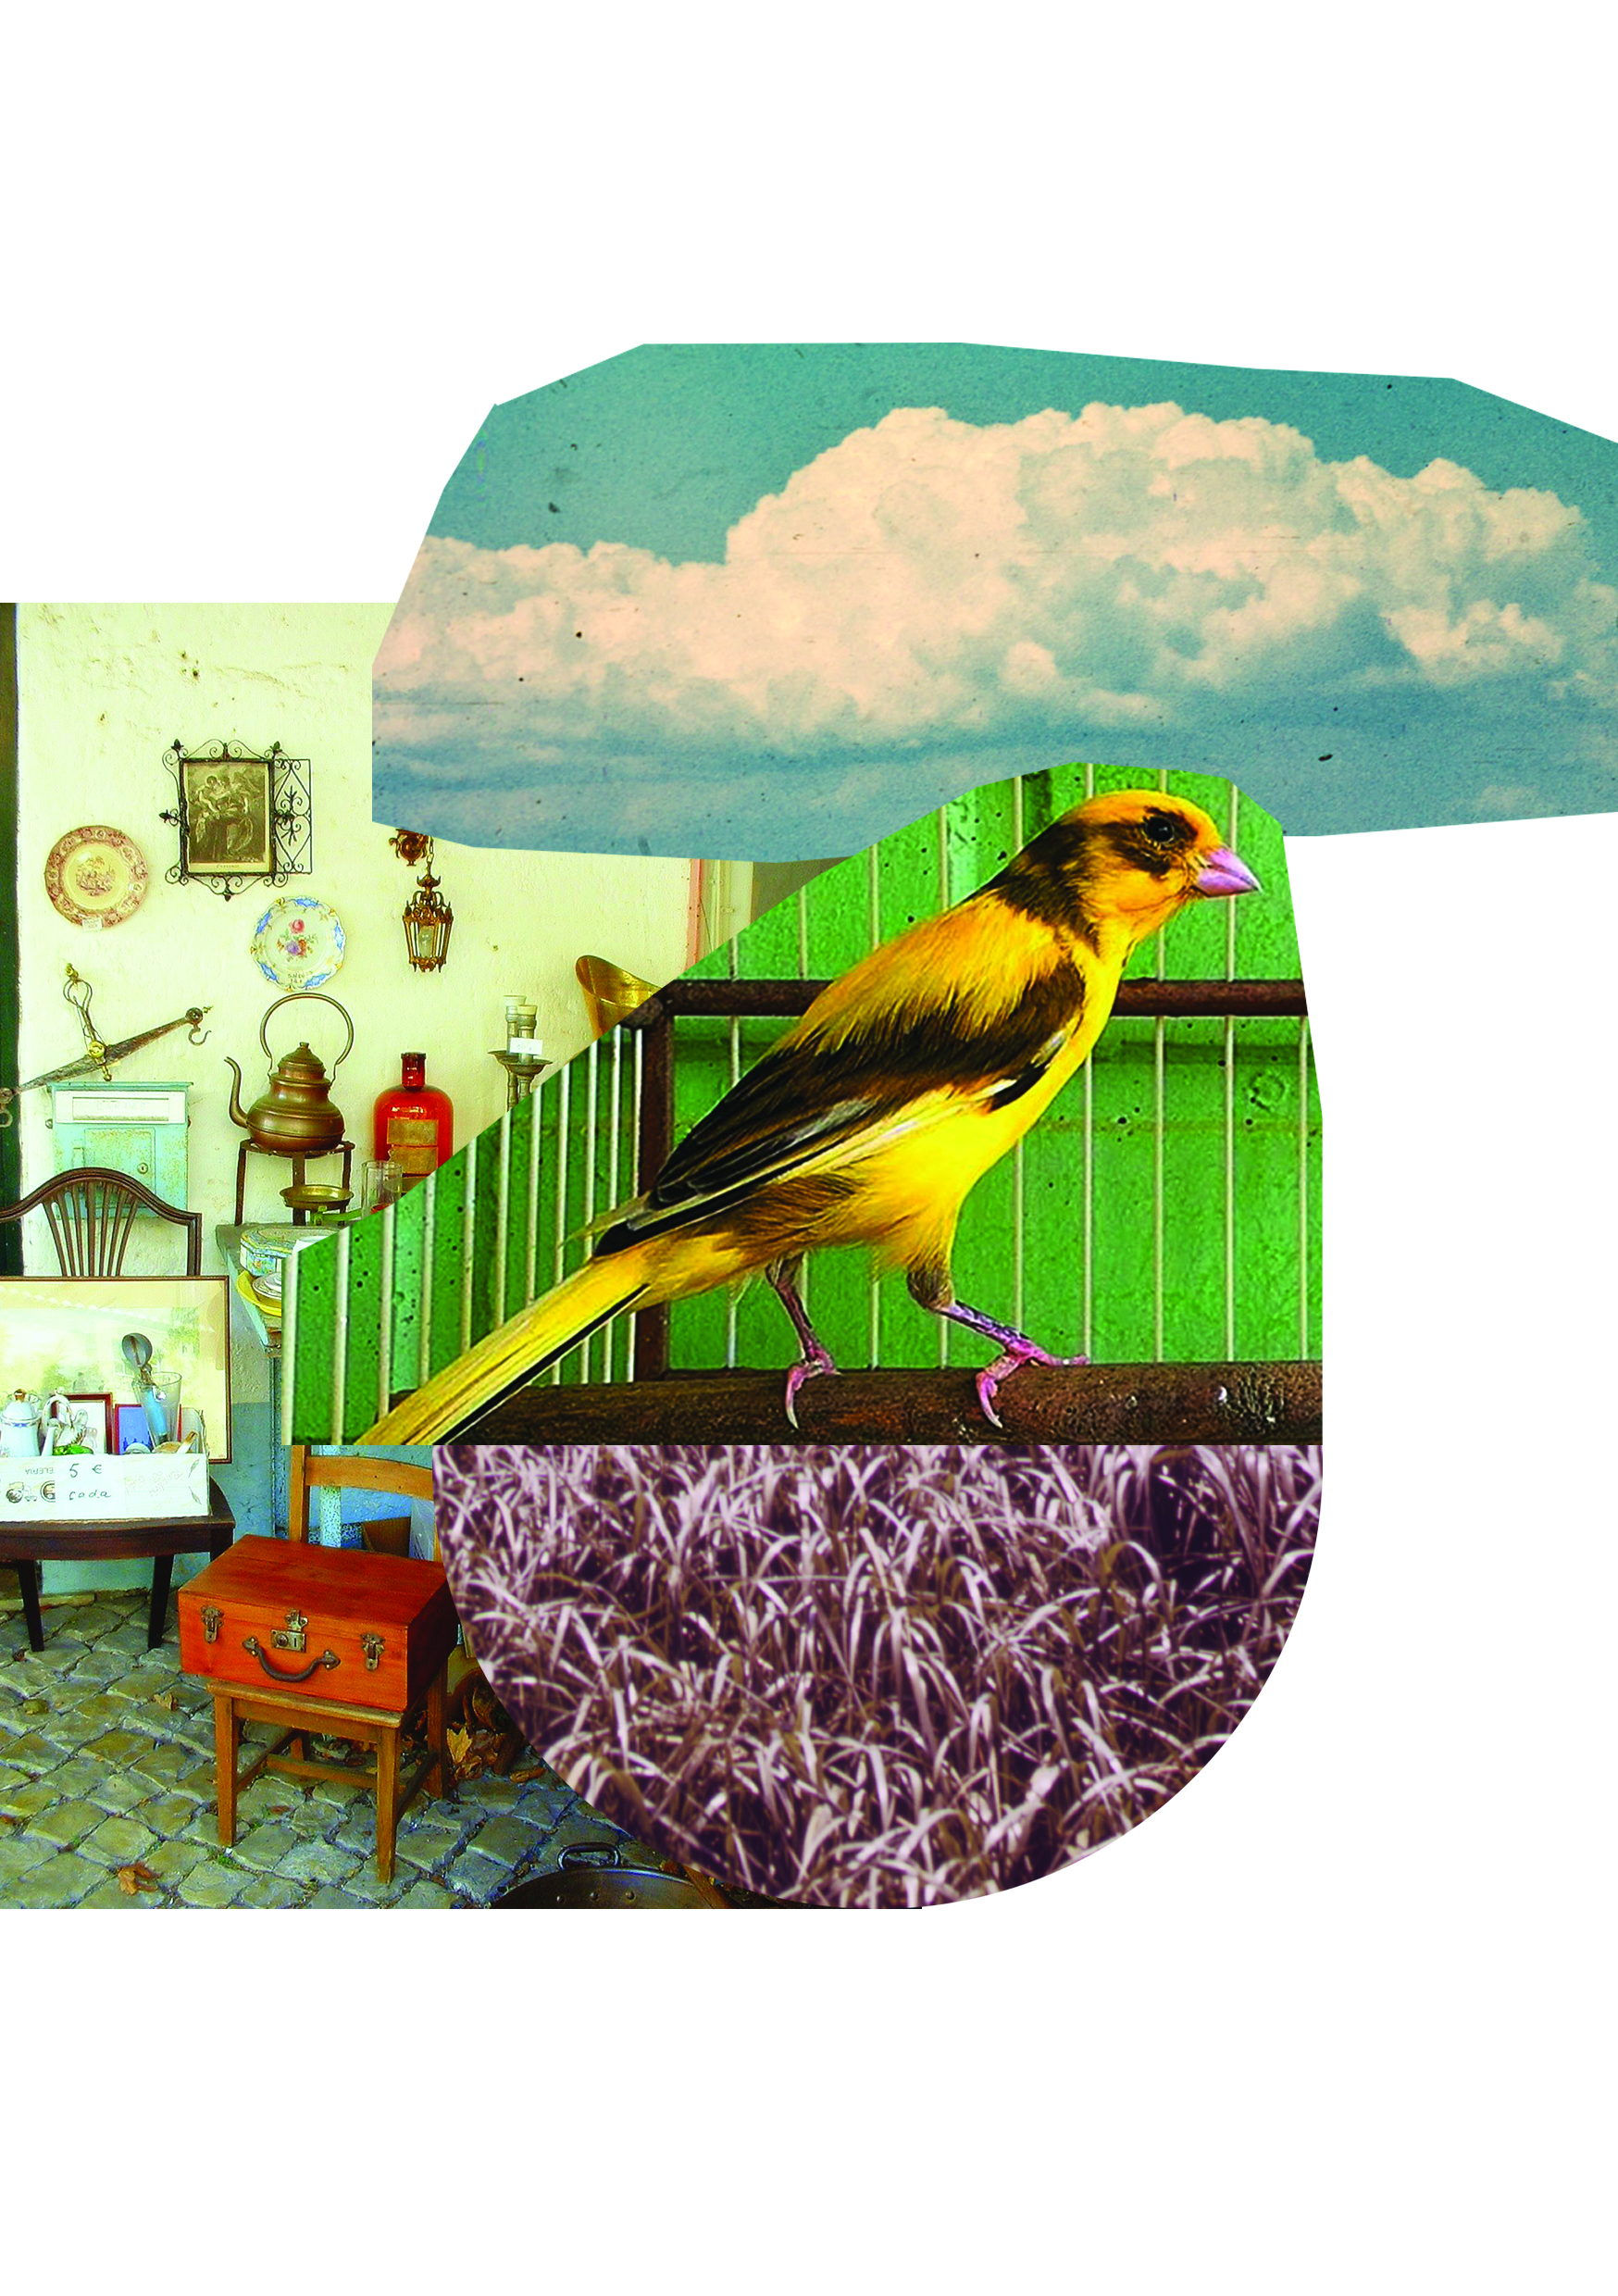
\includegraphics[width=140mm]{../ilustracoes/17_CANARIO.jpg}
\end{figure}
\pagebreak

\chapterspecial{Ideias de canário}{}{Machado de Assis}

\noindent{}Um homem dado a estudos de ornitologia, por nome Macedo, referiu a
alguns amigos um caso tão extraordinário que ninguém lhe deu crédito.
Alguns chegam a supor que Macedo virou o juízo. Eis aqui o resumo da
narração.

No princípio do mês passado --- disse ele ---, indo por uma rua, sucedeu
que um tílburi à disparada, quase me atirou ao chão. Escapei saltando
para dentro de uma loja de belchior.\footnote{belchior: negociante de
  roupas e objetos usados.} Nem o estrépito do cavalo e do veículo, nem
a minha entrada fez levantar o dono do negócio, que cochilava ao fundo,
sentado numa cadeira de abrir. Era um frangalho de homem, barba cor de
palha suja, a cabeça enfiada em um gorro esfarrapado, que provavelmente
não achara comprador. Não se adivinhava nele nenhuma história, como
podiam ter alguns dos objetos que vendia, nem se lhe sentia a tristeza
austera e desenganada das vidas que foram vidas.

A loja era escura, atulhada das cousas velhas, tortas, rotas,
enxovalhadas, enferrujadas, que de ordinário se acham em tais casas,
tudo naquela meia desordem própria do negócio. Essa mistura, posto que
banal, era interessante. Panelas sem tampa, tampas sem panela, botões,
sapatos, fechaduras, uma saia preta, chapéus de palha e de pelo,
caixilhos, binóculos, meias casacas, um florete, um cão empalhado, um
par de chinelas, luvas, vasos sem nome, dragonas, uma bolsa de veludo,
dous cabides, um bodoque, um termômetro, cadeiras, um retrato
litografado pelo finado Sisson, um gamão, duas máscaras de arame para o
carnaval que há de vir, tudo isso e o mais que não vi ou não me ficou de
memória, enchia a loja nas imediações da porta, encostado, pendurado ou
exposto em caixas de vidro, igualmente velhas. Lá para dentro, havia
outras cousas mais e muitas, e do mesmo aspecto, dominando os objetos
grandes, cômodas, cadeiras, camas, uns por cima dos outros, perdidos na
escuridão.

Ia a sair, quando vi uma gaiola pendurada da porta. Tão velha como o
resto, para ter o mesmo aspecto da desolação geral, faltava-lhe estar
vazia. Não estava vazia. Dentro pulava um canário. A cor, a animação e a
graça do passarinho davam àquele amontoado de destroços uma nota de vida
e de mocidade. Era o último passageiro de algum naufrágio, que ali foi
parar íntegro e alegre como dantes. Logo que olhei para ele, entrou a
saltar mais, abaixo e acima, de poleiro em poleiro, como se quisesse
dizer que no meio daquele cemitério brincava um raio de sol. Não atribuo
essa imagem ao canário, senão porque falo a gente retórica; em verdade,
ele não pensou em cemitério nem sol, segundo me disse depois. Eu, de
envolta com o prazer que me trouxe aquela vista, senti-me indignado do
destino do pássaro, e murmurei baixinho palavras de azedume.

--- Quem seria o dono execrável\footnote{execrável: detestável,
  deplorável.} deste bichinho, que teve ânimo de se desfazer dele por
alguns pares de níqueis? Ou que mão indiferente, não querendo guardar
esse companheiro de dono defunto, o deu de graça a algum pequeno, que o
vendeu para ir jogar uma quiniela?

E o canário, quedando-se em cima do poleiro, trilou isto:

--- Quem quer que sejas tu, certamente não estás em teu juízo. Não tive
dono execrável, nem fui dado a nenhum menino que me vendesse. São
imaginações de pessoa doente; vai-te curar, amigo\ldots{}

--- Como --- interrompi eu, sem ter tempo de ficar espantado. --- Então
o teu dono não te vendeu a esta casa? Não foi a miséria ou a ociosidade
que te trouxe a este cemitério, como um raio de sol?

--- Não sei que seja sol nem cemitério. Se os canários que tens visto
usam do primeiro desses nomes, tanto melhor, porque é bonito, mas estou
que confundes.

--- Perdão, mas tu não vieste para aqui à toa, sem ninguém, salvo se o
teu dono foi sempre aquele homem que ali está sentado.

--- Que dono? Esse homem que aí está é meu criado, dá-me água e comida
todos os dias, com tal regularidade que eu, se devesse pagar-lhe os
serviços, não seria com pouco; mas os canários não pagam criados. Em
verdade, se o mundo é propriedade dos canários, seria extravagante que
eles pagassem o que está no mundo.

Pasmado das respostas, não sabia que mais admirar, se a linguagem, se as
ideias. A linguagem, posto me entrasse pelo ouvido como de gente, saía
do bicho em trilos engraçados. Olhei em volta de mim, para verificar se
estava acordado; a rua era a mesma, a loja era a mesma loja escura,
triste e úmida. O canário, movendo a um lado e outro, esperava que eu
lhe falasse. Perguntei-lhe então se tinha saudades do espaço azul e
infinito\ldots{}

--- Mas, caro homem --- trilou\footnote{trilar: gorjear; cantar.} o
canário ---, que quer dizer espaço azul e infinito?

--- Mas, perdão, que pensas deste mundo? Que coisa é o mundo?

--- O mundo --- redarguiu o canário com certo ar de professor ---, o
mundo é uma loja de belchior, com uma pequena gaiola de taquara,
quadrilonga, pendente de um prego; o canário é senhor da gaiola que
habita e da loja que o cerca. Fora daí, tudo é ilusão e mentira.

Nisto acordou o velho, e veio a mim arrastando os pés. Perguntou-me se
queria comprar o canário. Indaguei se o adquirira, como o resto dos
objetos que vendia, e soube que sim, que o comprara a um barbeiro,
acompanhado de uma coleção de navalhas.

--- As navalhas estão em muito bom uso --- concluiu ele.

--- Quero só o canário.

Paguei-lhe o preço, mandei comprar uma gaiola vasta, circular, de
madeira e arame, pintada de branco, e ordenei que a pusessem na varanda
da minha casa, donde o passarinho podia ver o jardim, o repuxo e um
pouco do céu azul.

Era meu intuito fazer um longo estudo do fenômeno, sem dizer nada a
ninguém, até poder assombrar o século com a minha extraordinária
descoberta. Comecei por alfabetar a língua do canário, por estudar-lhe a
estrutura, as relações com a música, os sentimentos estéticos do bicho,
as suas ideias e reminiscências. Feita essa análise filológica e
psicológica, entrei propriamente na história dos canários, na origem
deles, primeiros séculos, geologia e flora das ilhas Canárias, se ele
tinha conhecimento da navegação, etc. Conversávamos longas horas, eu
escrevendo as notas, ele esperando, saltando, trilando.

Não tendo mais família que dois criados, ordenava-lhes que não me
interrompessem, ainda por motivo de alguma carta ou telegrama urgente,
ou visita de importância. Sabendo ambos das minhas ocupações
científicas, acharam natural a ordem, e não suspeitaram que o canário e
eu nos entendíamos.

Não é mister\footnote{mister: necessário, preciso.} dizer que dormia
pouco, acordava duas e três vezes por noite, passeava à toa, sentia-me
com febre. Afinal tornava ao trabalho, para reler, acrescentar, emendar.
Retifiquei mais de uma observação --- ou por havê-la entendido mal, ou
porque ele não a tivesse expresso claramente. A definição do mundo foi
uma delas. Três semanas depois da entrada do canário em minha casa,
pedi-lhe que me repetisse a definição do mundo.

--- O mundo --- respondeu ele --- é um jardim assaz largo com repuxo no
meio, flores e arbustos, alguma grama, ar claro e um pouco de azul por
cima; o canário, dono do mundo, habita uma gaiola vasta, branca e
circular, donde mira o resto. Tudo o mais é ilusão e mentira.

Também a linguagem sofreu algumas retificações, e certas conclusões, que
me tinham parecido simples, vi que eram temerárias. Não podia ainda
escrever a memória que havia de mandar ao Museu Nacional, ao Instituto
Histórico e às universidades alemãs, não porque faltasse matéria, mas
para acumular primeiro todas as observações e ratificá-las\footnote{ratificar:
  confirmar.}. Nos últimos dias, não saía de casa, não respondia a
cartas, não quis saber de amigos nem parentes. Todo eu era canário. De
manhã, um dos criados tinha a seu cargo limpar a gaiola e pôr-lhe água e
comida. O passarinho não lhe dizia nada, como se soubesse que a esse
homem faltava qualquer preparo científico. Também o serviço era o mais
sumário do mundo; o criado não era amador de pássaros.

Um sábado amanheci enfermo, a cabeça e a espinha doíam-me. O médico
ordenou absoluto repouso; era excesso de estudo, não devia ler nem
pensar, não devia saber sequer o que se passava na cidade e no mundo.
Assim fiquei cinco dias; no sexto levantei-me, e só então soube que o
canário, estando o criado a tratar dele, fugira da gaiola. O meu
primeiro gesto foi para esganar o criado; a indignação sufocou-me, caí
na cadeira, sem voz, tonto. O culpado defendeu-se, jurou que tivera
cuidado, o passarinho é que fugira por astuto\ldots{}

--- Mas não o procuraram?

--- Procuramos, sim, senhor; a princípio trepou ao telhado, trepei
também, ele fugiu, foi para uma árvore, depois escondeu-se não sei onde.
Tenho indagado desde ontem, perguntei aos vizinhos, aos chacareiros,
ninguém sabe nada.

Padeci muito; felizmente, a fadiga estava passada, e com algumas horas
pude sair à varanda e ao jardim. Nem sombra de canário. Indaguei, corri,
anunciei, e nada. Tinha já recolhido as notas para compor a memória,
ainda que truncada e incompleta, quando me sucedeu visitar um amigo, que
ocupa uma das mais belas e grandes chácaras dos arrabaldes. Passeávamos
nela antes de jantar, quando ouvi trilar esta pergunta:

--- Viva, Sr. Macedo, por onde tem andado que desapareceu?

Era o canário; estava no galho de uma árvore. Imaginem como fiquei, e o
que lhe disse. O meu amigo cuidou que eu estivesse doido; mas que me
importavam cuidados de amigos? Falei ao canário com ternura, pedi-lhe
que viesse continuar a conversação, naquele nosso mundo composto de um
jardim e repuxo, varanda e gaiola branca e circular\ldots{}

--- Que jardim? Que repuxo?

--- O mundo, meu querido.

--- Que mundo? Tu não perdes os maus costumes de professor. O mundo ---
concluiu solenemente --- é um espaço infinito e azul, com o sol por
cima.

Indignado, retorqui-lhe que, se eu lhe desse crédito, o mundo era tudo;
até já fora uma loja de belchior\ldots{}

--- De belchior? --- trilou ele às bandeiras despregadas. Mas há mesmo
lojas de belchior?




% Indice remissivo (package: `\usepackage{makeidx}` e no início do arquivi `\makeindex`
% \printindex

% Indice
% \renewcommand{\contentsname}{Índice}
% \setcounter{tocdepth}{3}
% \tableofcontents

% \endnotes

%PEGAR SEMPRE A VERSÃO ATUALIZADA DO REPOSITÓRIO "PUBLICIDADE"
\pagebreak
\blankpage
%\blankAteven
\pagestyle{empty}
\begingroup
\fontsize{7}{8}\selectfont

{\large\textsc{coleção «hedra edições»}}

\begin{enumerate}
\setlength\parskip{4.2pt}
\setlength\itemsep{-1.4mm}
%\item \textit{Poemas da cabana montanhesa}, Saigy\=o
\item \textit{A arte da guerra}, Maquiavel
\item \textit{A conjuração de Catilina}, Salústio
\item \textit{A cruzada das crianças/ Vidas imaginárias}, Marcel Schwob
\item \textit{A filosofia na era trágica dos gregos}, Friedrich Nietzsche
\item \textit{A fábrica de robôs}, Karel Tchápek 
\item \textit{A história trágica do Doutor Fausto}, Christopher Marlowe
\item \textit{A metamorfose}, Franz Kafka
\item \textit{A monadologia e outros textos}, Gottfried Leibniz
\item \textit{A morte de Ivan Ilitch}, Lev Tolstói 
\item \textit{A velha Izerguil e outros contos}, Maksim Górki
\item \textit{A vida é sonho}, Calderón de la Barca
\item \textit{A volta do parafuso}, Henry James
\item \textit{A voz dos botequins e outros poemas}, Paul Verlaine 
\item \textit{A vênus das peles}, Leopold von Sacher{}-Masoch
\item \textit{A última folha e outros contos}, O.\,Henry
\item \textit{Americanismo e fordismo}, Antonio Gramsci
\item \textit{Anarquia pela educação}, Élisée Reclus 
\item \textit{Apologia de Galileu}, Tommaso Campanella 
\item \textit{Arcana C\oe lestia} e \textit{Apocalipsis revelata}, Emanuel Swedenborg
\item \textit{As bacantes}, Eurípides
\item \textit{Autobiografia de uma pulga}, [Stanislas de Rhodes]
\item \textit{Ação direta e outros escritos}, Voltairine de Cleyre
\item \textit{Balada dos enforcados e outros poemas}, François Villon
\item \textit{Carmilla, a vampira de Karnstein}, Sheridan Le Fanu
\item \textit{Carta sobre a tolerância}, John Locke
\item \textit{Contos clássicos de vampiro}, L.\,Byron, B.\,Stoker \& outros
\item \textit{Contos de amor, de loucura e de morte}, Horacio Quiroga
\item \textit{Contos indianos}, Stéphane Mallarmé
\item \textit{Cultura estética e liberdade}, Friedrich von Schiller
\item \textit{Cântico dos cânticos}, [Salomão]
\item \textit{Dao De Jing}, Lao Zi
\item \textit{Discursos ímpios}, Marquês de Sade
\item \textit{Dissertação sobre as paixões}, David Hume
\item \textit{Diário de um escritor (1873)}, Fiódor Dostoiévski
\item \textit{Diário parisiense e outros escritos}, Walter Benjamin
\item \textit{Diários de Adão e Eva}, Mark Twain
\item \textit{Don Juan}, Molière
\item \textit{Dos novos sistemas na arte}, Kazimir Maliévitch
\item \textit{Educação e sociologia}, Émile Durkheim
\item \textit{Édipo Rei}, Sófocles
\item \textit{Elogio da loucura}, Erasmo de Rotterdam
\item \textit{Émile e Sophie ou os solitários}, Jean-Jacques Rousseau 
\item \textit{Emília Galotti}, Gotthold Ephraim Lessing
\item \textit{Entre camponeses}, Errico Malatesta
\item \textit{Ernestine ou o nascimento do amor}, Stendhal
\item \textit{Escritos revolucionários}, Errico Malatesta
\item \textit{Escritos sobre arte}, Charles Baudelaire
\item \textit{Escritos sobre literatura}, Sigmund Freud
\item \textit{Eu acuso!}, Zola/\,\textit{O processo do capitão Dreyfus}, Rui Barbosa
\item \textit{Explosão: romance da etnologia}, Hubert Fichte
\item \textit{Fedro}, Platão
\item \textit{Feitiço de amor e outros contos}, Ludwig Tieck
\item \textit{Flossie, a Vênus de quinze anos}, [Swinburne]
\item \textit{Fábula de Polifemo e Galateia e outros poemas}, Góngora
\item \textit{Fé e saber}, Georg W.\,F.\,Hegel
\item \textit{Gente de Hemsö}, August Strindberg 
\item \textit{Hawthorne e seus musgos}, Melville
\item \textit{Hino a Afrodite e outros poemas}, Safo de Lesbos 
\item \textit{História da anarquia (vol.\,\textsc{ii})}, Max Nettlau
\item \textit{História da anarquia (vol.\,\textsc{i})}, Max Nettlau
\item \textit{Imitação de Cristo}, Tomás de Kempis
\item \textit{Incidentes da vida de uma escrava}, Harriet Jacobs
\item \textit{Inferno}, August Strindberg
\item \textit{Investigação sobre o entendimento humano}, David Hume
\item \textit{Jazz rural}, Mário de Andrade
\item \textit{Jerusalém}, William Blake
\item \textit{Joana d'Arc}, Jules Michelet
\item \textit{Lira grega}, Giuliana Ragusa (org.)
\item \textit{Lisístrata}, Aristófanes 
\item \textit{Ludwig Feuerbach e o fim da filosofia clássica alemã}, Friederich Engels
\item \textit{Manifesto comunista}, Karl Marx e Friederich Engels
\item \textit{Memórias do subsolo}, Fiódor Dostoiévski
\item \textit{Metamorfoses}, Ovídio
\item \textit{Micromegas e outros contos}, Voltaire
\item \textit{Narrativa de William W.\,Brown, escravo fugitivo}, William Wells Brown
\item \textit{Nascidos na escravidão: depoimentos norte-americanos}, \textsc{wpa}
\item \textit{No coração das trevas}, Joseph Conrad
\item \textit{Noites egípcias e outros contos}, Aleksandr Púchkin
\item \textit{O casamento do Céu e do Inferno}, William Blake
\item \textit{O cego e outros contos}, \textsc{d.\,h}.\,Lawrence
\item \textit{O chamado de Cthulhu}, \textsc{h.\,p.}\,lovecraft
\item \textit{O contador de histórias e outros textos}, Walter Benjamin
\item \textit{O corno de si próprio e outros contos}, Marquês de Sade
\item \textit{O destino do erudito}, Johann Fichte
\item \textit{O estranho caso do dr.\,Jekyll e Mr. Hyde}, Robert Louis Stevenson
\item \textit{O fim do ciúme e outros contos}, Marcel Proust
\item \textit{O indivíduo, a sociedade e o Estado, e outros ensaios}, Emma Goldman
\item \textit{O ladrão honesto e outros contos}, Fiódor Dostoiévski
\item \textit{O livro de Monelle}, Marcel Schwob
\item \textit{O mundo ou tratado da luz}, René Descartes
\item \textit{O novo Epicuro: as delícias do sexo}, Edward Sellon
\item \textit{O pequeno Zacarias, chamado Cinábrio}, \textsc{e.\,t.\,a.}\,Hoffmann
\item \textit{O primeiro Hamlet}, William Shakespeare
\item \textit{O princípio anarquista e outros ensaios}, Piotr Kropotkin
\item \textit{O princípio do Estado e outros ensaios}, Mikhail Bakunin
\item \textit{O príncipe}, Maquiavel
\item \textit{O que eu vi, o que nós veremos}, Santos-Dumont
\item \textit{O retrato de Dorian Gray}, Oscar Wilde
\item \textit{O sobrinho de Rameau}, Diderot
\item \textit{Ode ao Vento Oeste e outros poemas}, \textsc{p.\,b.}\,Shelley
\item \textit{Ode sobre a melancolia e outros poemas}, John Keats
\item \textit{Odisseia}, Homero
\item \textit{Oliver Twist}, Charles Dickens
\item \textit{Origem do drama barroco}, Walter Benjamin
\item \textit{Os sofrimentos do jovem Werther}, Goethe
\item \textit{Os sovietes traídos pelos bolcheviques}, Rudolf Rocker
\item \textit{Para serem lidas à noite}, Ion Minulescu
\item \textit{Pensamento político de Maquiavel}, Johann Fichte
\item \textit{Pequeno-burgueses}, Maksim Górki
\item \textit{Pequenos poemas em prosa}, Charles Baudelaire
\item \textit{Perversão: a forma erótica do ódio}, Robert Stoller
\item \textit{Poemas}, Lord Byron
\item \textit{Poesia basca: das origens à Guerra Civil} 
\item \textit{Poesia catalã: das origens à Guerra Civil} 
\item \textit{Poesia espanhola: das origens à Guerra Civil} 
\item \textit{Poesia galega: das origens à Guerra Civil} 
\item \textit{Pr\ae terita}, John Ruskin
\item \textit{Primeiro livro dos Amores}, Ovídio
\item \textit{Rashômon e outros contos}, Ryūnosuke Akutagawa
\item \textit{Revolução e liberdade: cartas de 1845 a 1875}, Mikhail Bakunin
\item \textit{Robinson Crusoé}, Daniel Defoe
\item \textit{Romanceiro cigano}, Federico García Lorca
\item \textit{Sagas}, August Strindberg
\item \textit{Sobre a amizade e outros diálogos}, Jorge Luis Borges e Osvaldo Ferrari
\item \textit{Sobre a filosofia e outros diálogos}, Jorge Luis Borges e Osvaldo Ferrari
\item \textit{Sobre a filosofia e seu método (Parerga e paralipomena)} (v.\textsc{ii}, t.\textsc{i}), Arthur Schopenhauer 
\item \textit{Sobre a liberdade}, Stuart Mill
\item \textit{Sobre a utilidade e a desvantagem da histório para a vida}, Friedrich Nietzsche
\item \textit{Sobre a ética (Parerga e paralipomena)} (v.\textsc{ii}, t.\textsc{ii}), Arthur Schopenhauer 
\item \textit{Sobre anarquismo, sexo e casamento}, Emma Goldman
\item \textit{Sobre o riso e a loucura}, [Hipócrates]
\item \textit{Sobre os sonhos e outros diálogos}, Jorge Luis Borges e Osvaldo Ferrari
\item \textit{Sobre verdade e mentira}, Friedrich Nietzsche
\item \textit{Sonetos}, William Shakespeare
\item \textit{Sátiras, fábulas, aforismos e profecias}, Leonardo da Vinci
\item \textit{Teleny, ou o reverso da medalha}, Oscar Wilde
\item \textit{Teogonia}, Hesíodo
\item \textit{Trabalhos e dias}, Hesíodo
\item \textit{Triunfos}, Petrarca
\item \textit{Um anarquista e outros contos}, Joseph Conrad
\item \textit{Viagem aos Estados Unidos}, Alexis de Tocqueville
\item \textit{Viagem em volta do meu quarto}, Xavier de Maistre 
\item \textit{Viagem sentimental}, Laurence Sterne
\end{enumerate}

% {\large\textsc{coleção «metabiblioteca»}}

% \begin{enumerate}
% \setlength\parskip{4.2pt}
% \setlength\itemsep{-1.4mm}
% \item \textit{A carteira de meu tio}, Joaquim Manuel de Macedo
% \item \textit{A cidade e as serras}, Eça de Queirós
% \item \textit{A escrava}, Maria Firmina dos Reis
% \item \textit{A família Medeiros}, Júlia Lopes de Almeida 
% \item \textit{A pele do lobo e outras peças}, Artur Azevedo
% \item \textit{Auto da barca do inferno}, Gil Vicente
% \item \textit{Bom crioulo}, Adolfo Caminha
% \item \textit{Cartas a favor da escravidão}, José de Alencar
% \item \textit{Contos e novelas}, Júlia Lopes de Almeida
% \item \textit{Crime}, Luiz Gama
% \item \textit{Democracia}, Luiz Gama
% \item \textit{Direito}, Luiz Gama
% \item \textit{Elixir do pajé: poemas de humor, sátira e escatologia}, Bernardo Guimarães
% \item \textit{Eu}, Augusto dos Anjos
% \item \textit{Farsa de Inês Pereira}, Gil Vicente
% \item \textit{Helianto}, Orides Fontela
% \item \textit{História da província Santa Cruz}, Gandavo
% \item \textit{Iracema}, José de Alencar
% \item \textit{Liberdade}, Luiz Gama
% \item \textit{Mensagem}, Fernando Pessoa
% \item \textit{Meridiano 55}, Flávio de Carvalho
% \item \textit{O Ateneu}, Raul Pompeia
% \item \textit{O cortiço}, Aluísio Azevedo
% \item \textit{O desertor}, Silva Alvarenga
% \item \textit{Oração aos moços}, Rui Barbosa
% \item \textit{Pai contra mãe e outros contos}, Machado de Assis
% \item \textit{Poemas completos de Alberto Caeiro}, Fernando Pessoa
% \item \textit{Teatro de êxtase}, Fernando Pessoa
% \item \textit{Transposição}, Orides Fontela
% \item \textit{Tratado descritivo do Brasil em 1587}, Gabriel Soares de Sousa
% \item \textit{Tratados da terra e gente do Brasil}, Fernão Cardim 
% \item \textit{Utopia Brasil}, Darcy Ribeiro
% \item \textit{Índice das coisas mais notáveis}, Antônio Vieira
% \end{enumerate}

% \medskip
% {\large\textsc{coleção «que horas são?»}}

% \begin{enumerate}
% \setlength\parskip{4.2pt}
% \setlength\itemsep{-1.4mm}
% \item \textit{8/1: A rebelião dos manés}, Pedro Fiori Arantes, Fernando Frias e Maria Luiza Meneses
% \item \textit{A linguagem fascista}, Carlos Piovezani \& Emilio Gentile
% \item \textit{A sociedade de controle}, J.\,Souza; R.\,Avelino; S.\,Amadeu (orgs.)
% \item \textit{Ativismo digital hoje}, R.\,Segurado; C.\,Penteado; S.\,Amadeu (orgs.)
% \item \textit{Crédito à morte}, Anselm Jappe
% \item \textit{Descobrindo o Islã no Brasil}, Karla Lima
% \item \textit{Desinformação e democracia}, Rosemary Segurado
% \item \textit{Dilma Rousseff e o ódio político}, Tales Ab'Sáber
% \item \textit{Labirintos do fascismo} (v.\textsc{iii}), João Bernardo
% \item \textit{Labirintos do fascismo} (v.\textsc{ii}), João Bernardo
% \item \textit{Labirintos do fascismo} (v.\textsc{iv}), João Bernardo
% \item \textit{Labirintos do fascismo} (v.\textsc{i}), João Bernardo
% \item \textit{Labirintos do fascismo} (v.\textsc{vi}), João Bernardo
% \item \textit{Labirintos do fascismo} (v.\textsc{v}), João Bernardo
% \item \textit{Lugar de negro, lugar de branco?}, Douglas Rodrigues Barros
% \item \textit{Lulismo, carisma pop e cultura anticrítica}, Tales Ab'Sáber
% \item \textit{Machismo, racismo, capitalismo identitário}, Pablo Polese
% \item \textit{Michel Temer e o fascismo comum}, Tales Ab'Sáber
% \item \textit{O quarto poder: uma outra história}, Paulo Henrique Amorim
% \item \textit{Universidade, cidade e cidadania}, Franklin Leopoldo e Silva
% \end{enumerate}

% \medskip
% {\large\textsc{coleção «mundo indígena»}}

% \begin{enumerate}
% \setlength\parskip{4.2pt}
% \setlength\itemsep{-1.4mm}
% \item \textit{A folha divina}, Timóteo Verá Tupã Popygua
% \item \textit{A mulher que virou tatu}, Eliane Camargo
% \item \textit{A terra uma só}, Timóteo Verá Tupã Popygua
% \item \textit{A árvore dos cantos}, Pajés Parahiteri
% \item \textit{Cantos dos animais primordiais}, Ava Ñomoandyja Atanásio Teixeira
% \item \textit{Crônicas de caça e criação}, Uirá Garcia
% \item \textit{Círculos de coca e fumaça}, Danilo Paiva Ramos
% \item \textit{Nas redes guarani}, Valéria Macedo \& Dominique Tilkin-Gallois
% \item \textit{Não havia mais homens}, Luciana Storto
% \item \textit{O surgimento da noite}, Pajés Parahiteri
% \item \textit{O surgimento dos pássaros}, Pajés Parahiteri
% \item \textit{Os Aruaques}, Max Schmidt
% \item \textit{Os cantos do homem-sombra}, Patience Epps e Danilo Paiva Ramos
% \item \textit{Os comedores de terra}, Pajés Parahiteri
% \item \textit{Xamanismos ameríndios}, A.\,Barcelos Neto, L.\,Pérez Gil \& D.\,Paiva Ramos
% \end{enumerate}

% \medskip
% {\large\textsc{coleção «ecopolítica»}}

% \begin{enumerate}
% \setlength\parskip{4.2pt}
% \setlength\itemsep{-1.4mm}
% \item \textit{Anarquistas na América do Sul}, E.\,Passetti, S.\,Gallo; A.\,Augusto  (orgs.)
% \item \textit{Ecopolítica}, E.\,Passetti; A.\,Augusto; B.\,Carneiro; S.\,Oliveira, T.\,Rodrigues  (orgs.)
% \item \textit{Pandemia e anarquia}, E.\,Passetti; J.\,da Mata; J.\,Ferreira  (orgs.)
% \end{enumerate}

% % \medskip
% % {\large\textsc{coleção <<anarc>>}}

% % \begin{enumerate}
% % \setlength\parskip{4.2pt}
% % \setlength\itemsep{-1.4mm}
% % \item \textit{Anarquia pela educação}, Élisée Reclus 
% % \item \textit{Ação direta e outros escritos}, Voltairine de Cleyre
% % \item \textit{Entre camponeses}, Errico Malatesta
% % \item \textit{Escritos revolucionários}, Errico Malatesta
% % \item \textit{História da anarquia (vol.\,\textsc{ii})}, Max Nettlau
% % \item \textit{História da anarquia (vol.\,\textsc{i})}, Max Nettlau
% % \item \textit{O indivíduo, a sociedade e o Estado, e outros ensaios}, Emma Goldman
% % \item \textit{O princípio anarquista e outros ensaios}, Piotr Kropotkin
% % \item \textit{O princípio do Estado e outros ensaios}, Mikhail Bakunin
% % \item \textit{Os sovietes traídos pelos bolcheviques}, Rudolf Rocker
% % \item \textit{Revolução e liberdade: cartas de 1845 a 1875}, Mikhail Bakunin
% % \item \textit{Sobre anarquismo, sexo e casamento}, Emma Goldman
% % \end{enumerate}

% % \medskip
% % {\large\textsc{coleção <<narrativas da escravidão>>}}

% % \begin{enumerate}
% % \setlength\parskip{4.2pt}
% % \setlength\itemsep{-1.4mm}
% % \item \textit{Incidentes da vida de uma escrava}, Harriet Jacobs
% % \item \textit{Narrativa de William W.\,Brown, escravo fugitivo}, William Wells Brown
% % \item \textit{Nascidos na escravidão: depoimentos norte-americanos}, \textsc{wpa}
% % \end{enumerate}


 \pagebreak	   % [lista de livros publicados]
%!TEX root=./LIVRO.tex
\pagebreak

\ifodd\thepage\blankpage\fi

\mbox{}\vfill


\begin{center}
		\begin{minipage}{.7\textwidth}\tiny\noindent{}
		\centering\tiny
		Adverte-se aos curiosos que se imprimiu este 
		livro
		% na gráfica Meta Brasil, 
		em \today{} em papel pólen soft, em tipologia Minion Pro e Formular, 
		com diversos sofwares livres, 
		entre eles, Lua\LaTeX, git.\\ 
		\ifdef{\RevisionInfo{}}{\par(v.\,\RevisionInfo)}{}\medskip\\\
		\adforn{64}
		\end{minipage}
\end{center}		   % [colofon]
